%%%%%%%%%%%%%%%%%%%%%%%%%%%%%%%%%%%%%%%%%%%%%%%%%%%%%%%%
%   |-------------------------|                        %
%   |REDES PRIVADAS VIRTUALES |                        %
%   |                         |                        %
%   | Proyecto de graduaci�n  |                        %
%   |_________________________|                        %
%                                                      %
%   Autores                                            %
%   -------                                            %
%                                                      %
% * Formoso Requena, Nicol�s Federico (CX02-0239-8)    %
%     nicolasformoso@gmail.com                         %
% * Cortez, Gustavo Maximiliano (CX01-0801-9)          %
%     cmgustavo83@gmail.com                            %
%                                                      %
%   Tutores                                            %
%   -------                                            %
%                                                      %
% * Ing. Gustavo Vanetta - vanettag@gmail.com          %
% * Lic. Miguel Bazzano - miguelbazzano@gmail.com      %
%                                                      %
%%%%%%%%%%%%%%%%%%%%%%%%%%%%%%%%%%%%%%%%%%%%%%%%%%%%%%%%

% ********* Informe principal ********** %

%% Clase del documento tipo reporte
\documentclass[a4paper]{report}

%% Paquetes adicionales
\usepackage[spanish,activeacute]{babel}			% Soporte spanish
\usepackage[spanish]{translator}
\usepackage[latin1]{inputenc}		% Entradas con acentos, e�es, etc
\usepackage{float}					% Para agregar imagenes fijas
\usepackage{latexsym} 				% S�mbolos
\usepackage{graphicx} 				% Inclusi�n de gr�ficos
\usepackage[pdftex=true,colorlinks=true,plainpages=true]{hyperref} % Soporte hipertexto
\usepackage{anysize} 				% Soporte para el comando \marginsize
\usepackage{makeidx} 				% Soporte de indices alfabeticos
\usepackage[none]{tocbibind} % Agregar bibliograf�a, indices, etc. al indice general
\usepackage{color}					% Uso de colores
\usepackage{listings}				% Para gregar listas personalizadas (codigos)
\usepackage{array}					% para que funcionen los par�metros m de \begin{tabular}
\usepackage{alltt}					% Extension de verbatim para usar comandos latex.
\usepackage{fancyhdr}				% Incluye encabezados y pie de p�ginas m�s complejos.
\usepackage{glossaries}     % Incluye glosario de t�rminos t�cnicos.

%% Definici�n de colores grises
\definecolor{gray99}{gray}{.99}
\definecolor{gray97}{gray}{.97}
\definecolor{gray85}{gray}{.85}
\definecolor{gray75}{gray}{.75}
\definecolor{gray45}{gray}{.45}

%% Lista personalizada para c�digos y configuraciones.
\lstset{ frame=Ltb,
     framerule=0pt,
     aboveskip=0.5cm,
     framextopmargin=3pt,
     framexbottommargin=3pt,
     framexleftmargin=0cm,
     framesep=0pt,
     rulesep=.4pt,
     backgroundcolor=\color{gray97},
     rulesepcolor=\color{black},
     stringstyle=\ttfamily,
     showstringspaces = false,
     basicstyle=\small\ttfamily,
     commentstyle=\color{gray45},
     keywordstyle=\bfseries,
     numbers=left,
     numbersep=5pt,
     numberstyle=\tiny,
     numberfirstline = false,
     breaklines=true,
   }
 
\lstnewenvironment{listing}[1][]
   {\lstset{#1}\pagebreak[0]}{\pagebreak[0]}
 
\lstdefinestyle{consola}
   {basicstyle=\scriptsize\bf\ttfamily,
    backgroundcolor=\color{gray85},
   }
   
\lstdefinestyle{configuracion}
   {basicstyle=\small\bf\ttfamily,
    backgroundcolor=\color{gray97},
   }
\lstdefinestyle{configuracion_small}	% Lo mismo que arriba pero m�s chiquito
   {basicstyle=\footnotesize\bf\ttfamily,
    backgroundcolor=\color{gray97},
   }

\lstdefinestyle{TeX}
   {language=TeX,
   }
   
\lstdefinestyle{bash}
   {language=bash,
   }

%% Definici�n de los c�digos, configuraciones y logs flotantes.
%% Codigos Latex
\floatstyle{plain}
\newfloat{codigo}{thb}{lop}
\floatname{codigo}{C�digo}
%% Codigos de configuraci�n
\floatstyle{ruled}
\newfloat{configuracion}{thb}{lop}
\floatname{configuracion}{Configuraci�n}
%
\newfloat{configuracion_small}{htb}{lop}
\floatname{configuracion_small}{Detalle}
%% Cuadros de registros (logs)
\floatstyle{boxed}
\newfloat{logs}{thb}{lop}
\floatname{logs}{Registro}

%% Definici�n de los m�rgenes
%% {margen_izq}{margen_dch}{margen_sup}{margen_inf}
%\marginsize{3cm}{2cm}{2.5cm}{2.5cm}

%% Espaciado entre lineas
%\baselinestretch{2.0}

%% Para la ruptura de palabras
% \hyphenation{O\-pe\-ra\-ti\-vo}
\hyphenation{in-me-dia-ta-men-te es-ta-ble-ci-mien-to PPPD co-rres-pon-dien-te trans-fe-ren-cia con-fi-gu-rar cre-ci-mien-to an-te-rior-men-te ad-mi-nis-tra-dor cui-da-do-sa-men-te en-crip-ta-dos Au-then-ti-ca-tion con-si-de-ra-dos in-te-gran-tes de-sa-rro-llo}

%% Encabezados y pie de p�gina
\pagestyle{headings}

%% T�tulo, autor y fecha
\title{Investigaci�n e Implementaci�n de Redes Privadas Virtuales}
\author{\href{mailto:cmgustavo83@gmail.com}{Gustavo Maximiliano Cortez}\\
\href{mailto:nicolasformoso@gmail.com}{Nicol�s Federico Formoso Requena}}
\date{2008}

% Diccionario de t�rminos t�cnicos (glosario)

% Generar el glosario por cada entrada nueva, con el comando (vieja no saques esa l�nea por favor):
%makeindex -s informe.ist -t informe.glg -o informe.gls informe.glo

\makeglossaries
%%%%%%%%%%%%%%%%%%%%%%%%%%%%%%%%%%%%%%%%%%%%%%%%%%%%%%%%
%   |-------------------------|                        %
%   |REDES PRIVADAS VIRTUALES |                        %
%   |                         |                        %
%   | Proyecto de graduaci�n  |                        %
%   |_________________________|                        %
%                                                      %
%   Autores                                            %
%   -------                                            %
%                                                      %
% * Formoso Requena, Nicol�s Federico (CX02-0239-8)    %
%     nicolasformoso@gmail.com                         %
% * Cortez, Gustavo Maximiliano (CX01-0801-9)          %
%     cmgustavo83@gmail.com                            %
%                                                      %
%   Tutores                                            %
%   -------                                            %
%                                                      %
% * Ing. Gustavo Vanetta - vanettag@gmail.com          %
% * Lic. Miguel Bazzano - miguelbazzano@gmail.com      %
%                                                      %
%%%%%%%%%%%%%%%%%%%%%%%%%%%%%%%%%%%%%%%%%%%%%%%%%%%%%%%%

% ********* Glosario ********** %

%% Formato general
%\newglossaryentry{<label>}{<key-val list>} 

%% Ejemplo
%\newglossaryentry{set}% the label
%{name=set,            % the term
% description={a collection of objects} % a brief description
%}

\newglossaryentry{VPN}
{name=VPN,
 description={Virtual Private Network, que en castellano se traduce a Red Privada Virtual o RPV, que se refiere a la conexi�n de redes locales en una sola gran red a trav�s de un canal seguro y fiable, atravezando un medio hostil como Internet.}
 }
 
\newglossaryentry{Subversion}
{name=Subversion,
 description={Sistema de control de versiones para el desarrollo colectivo de software o documentaci�n.}
 }
 
\newglossaryentry{TortoiseSVN}
{name=TortoriseSVN,
 description={Cliente Subversion para Windows que se agrega al men� contextual del sistema cuando se trabaja con el explorador.}
 }
 
\newglossaryentry{Ethernet}
{name=Ethernet,
 description={Especificaci�n de red de �rea local (LAN) desarrollada en 1976 por Xerox, en cooperaci�n con DEC e Intel, originalmente para conectar los miniordenadores del Palo Alto Research Center (EEUU).}
 }
 
\newglossaryentry{IPSec}
{name=IPSec (Internet Protocol Security),
 description={Es la abreviaci�n de IP Security (seguridad IP), que es un conjunto de protocolos dise�ados para asegurar el tr�fico sobre el protocolo IP.}
 }
 
\newglossaryentry{AH}
{name=AH (Authentication Header),
 description={Parte del conjunto de protocolos de IPSec que ofrece servicios de autenticaci�n de los paquetes IP.}
 }
 
\newglossaryentry{DNS}
{name=DNS (Domain Name Services),
 description={Abreviaci�n de Domain Name Service, que permite la resoluci�n de nombres f�cil de recordar en direcciones IP.}
 }
 
\newglossaryentry{OpenBSD}
{name=OpenBSD,
 description={Sistema Operativo (monol�tico) tipo Unix basado en el sistema 4.4BSD proveniente de NetBSD a raiz de discuciones filos�ficas.}
 }
 
\newglossaryentry{VNC}
{name=VNC (Virtual Network Computing),
 description={Es un sistema de visualizaci�n y control de escritorio remoto desarrollado por AT\&T, que actualmente hasta permite la transferencia de archivos.}
 }
 
\newglossaryentry{ESP}
{name=ESP (Encapsulating Security Payload),
 description={Parte del conjunto de protocolos IPSec que permite el encapsulado de informaci�n �til, obteniendo servicios como confidencialidad y autenticaci�n de paquetes IP.}
 }
 
\newglossaryentry{IPv4}
{name=IPv4 (Internet Protocol versi�n 4),
 description={Versi�n 4 del protocolo IP que se utiliza en Internet y permiti� el crecimiento del mismo. Este protocolo utiliza direcciones de 32 bits, asignadas a cada equipo conectado. Adem�s se tienen direcciones espec�ficas para uso en redes de area local.}
 }
 
\newglossaryentry{IPv6}
{name=IPv6 (Internet Protocol versi�n 6),
 description={Es la nueva versi�n del protocolo IP, que entre otras mejoras, utiliza direcciones de 128 bits permitiendo mayor cantidad de conexiones simult�neas. Adem�s en IPv6 se tiene IPSec como tecnolog�a obligatoria.}
 }
 
\newglossaryentry{LAN}
{name=LAN (Local Area Network),
 description={Es la tecnolog�a usada en redes internas que permiten comunicar m�ltiples sistemas a un medio compartido. Entre sus caracter�sticas se pueden destacar el ancho de banda total elevado, bajo retardo de transmisi�n, baja tasa de error y adem�s se trata de una red de propiedad privada.}
 }
 
\newglossaryentry{IPCOMP}
{name=IPCOMP (IP Payload Compression Protocol),
 description={Es un protocolo de compresi�n de bajo nivel para datagramas IP definido en la RFC 3173. Se utiliza para reducir el tama�o de datos transmitidos y ahorrar ancho de banda o mejorar conexiones de baja velocidad.}
 }
 
\newglossaryentry{SPD}
{name=SPD (Security Policy Database),
 description={Es una base de datos con normativas de seguridad que utiliza IPSec para comprobar qu� hacer con paquetes IP salientes.}
 }
 
 \newglossaryentry{SA}
{name=SA (Security Association),
 description={La asociaci�n de seguridad determina qu� par�metros espec�ficos utilizar para proteger los paquetes. Se pueden configurar de forma manual o autom�tica (mediante IKE), siendo esta �ltima la mejor opci�n cuando se tiene una red muy grande.}
 }
 
\newglossaryentry{SPI}
{name=SPI (Security Parameters Index),
 description={�ndice de par�metros de seguridad es solo un n�mero de 32 bits que se uiliza de �ndice en la recepci�n de paquetes IP mediante IPSec.}
 }
 
\newglossaryentry{SAD}
{name=SAD (Security Associations Database),
 description={La base de datos de asociaciones de seguridad forma parte de IPSec y contiene informaci�n confidencial como claves, n�meros de secuencia, etc.}
 }
 
\newglossaryentry{ISAKMP}
{name=ISAKMP (Internet Security Association and Key Management Protocol),
 description={Protocolo de gesti�n de claves y asociaci�n de seguridad de Internet que se utiliza para gestionar el intercambio de claves entre equipos de una VPN con IPSec.}
 }
 
\newglossaryentry{IKE}
{name=IKE (Internet Key Exchange Protocol),
 description={El protocolo de intercambio de claves de internet es un protocolo que combina elementos, definiciones y funcionalidad de protocolos como ISAKMP, SKEME y Oakley. Se utiliza en el marco de autentificaci�n entre pares en redes VPN con IPSec.}
 }
 
\newglossaryentry{SKEME}
{name=SKEME (Secure Key Exchange Mechanism),
 description={Mecanismo de intercambio de claves seguras, cuya funcionalidad se utiliza en el protocolo IKE para el establecimiento de VPN con IPSec.}
 }
 
\newglossaryentry{Oakley}
{name=Oakley (Oakley Key Determination Protocol),
 description={Protocolo que permite el intercambio de claves entre partes mediante el algoritmo Diffie-Hellman, utilizado para establecer VPN con IPSec.}
 }
 
\newglossaryentry{PFS}
{name=PFS (Perfect Fordward Secrecy),
 description={Secreto de env�o perfecto es una caracter�stica que implementa IKE para evitar que todos datos cifrados esten comprometidos cuando la clave lo est�. En este caso solamente estar�n comprometidos los datos cifrados con esa clave, no los dem�s.}
 }
 
\newglossaryentry{PSK}
{name=PSK (Pre-Shared Key),
 description={Clave pre-compartida es un m�todo de autenticaci�n utilizado en la Fase I por el protocolo IKE para establecer una comunicaci�n VPN con IPSec.}
 }

\newglossaryentry{PPTP}
{name=PPTP (Point to Point Tunneling Protocol),
 description={El protocolo punto a punto mediante t�nel ha sido desarrollado por un conjunto de empresas cuyo objetivo consist�a en utilizar el viejo protocolo conocido PPP para realizar conexiones punto a punto seguras bajo el protocolo TCP/IP.}
 }

\newglossaryentry{GRE}
{name=GRE (Generic Routing Encapsulation),
 description={Es un protocolo (n�mero 47) destinado al establecimiento de t�neles a trav�s de Internet. Se utiliza en para establecer conexiones VPN con PPTP o PPP.}
 }

\newglossaryentry{TCP}
{name=TCP (Transmission Control Protocol),
 description={Es un protocolo de comunicaci�n orientado a la conexi�n que trabaja en el nivel de transporte (capa 4) del modelo OSI. TCP a�ade las funciones necesarias para prestar un servicio libre de errores, sin p�rdidas y con seguridad en la comunicaci�n de dos sistemas.}
 }

\newglossaryentry{CHAP}
{name=CHAP (Challenge Handshake Authentication Protocol),
 description={Es un protocolo de autenticaci�n por desaf�o mutuo, que se usaba en comunicaciones PPP con el proveedor de servicios de Internet (ISP).}
 }

\newglossaryentry{MS-CHAP}
{name=MS-CHAP (Microsoft Challenge Handshake Authentication Protocol),
 description={Es la versi�n desarrollada por Microsoft del protocolo CHAP con numerosas diferencias. Existen dos versiones, la primera ha sido eliminada en Windows Vista, y la segunda versi�n, denominada MS-CHAPv2 fue introducida a partir de Windows 2000.}
 }

\newglossaryentry{MPPE}
{name=MPPE (Microsoft Point-to-Point Encryption),
 description={Es un protocolo utilizado para encriptar comunicaciones a trav�s de PPP y establecer enlaces VPN. Utiliza el algoritmo de encriptaci�n RSA RC4 y soporta llaves de 40, 56 y 128 bits, que se cambian regularmente para aumentar la seguridad.}
 }
 
\newglossaryentry{tcpdump}
{name=TCPdump,
 description={Software en modo texto que permite monitorear los paquetes que entran y salen de una interfaz de red. Fue desarrollado por Van Jacobson, Craig Leres and Steven McCanne. Esta herramienta es muy utilizada por administradores de red para la depuraci�n de errores y control de una red.}
 }

\newglossaryentry{Wireshark}
{name=Wireshark,
 description={Es una aplicaci�n de filtrado de paquetes de libre distribuci�n, con una amigable intrefaz gr�fica que permite monitorear el tr�fico de datos que entran y salen de una interfaz de red determinada. Esta es una derivaci�n de Ethereal desarrollado inicialmente por Lyle Roussel, y actualmente mantenido por una gran comunidad de usuarios y desarrolladores.}
 }
 
\newglossaryentry{traceroute}
{name=traceroute,
 description={Es un software libre desarrollado para sistemas tipo Unix que permite seguir el rastro de un paquete entre host origen y host destino.}
 }
 
\newglossaryentry{tracert}
{name=tracert,
 description={Es un software que viene con Windows (versi�n 2000 en adelante) que permite seguir el rastro de un paquete entre host origen y host destino.}
 }
 
\newglossaryentry{SMB}
{name=SMB (Server Message Block),
 description={Es un protocolo utilizado para compartir archivos, impresoras, puertos otros tipos de comunicaciones a trav�s de dos o m�s nodos de una red. Este opera en el nivel de aplicaci�n.}
 }
 
\newglossaryentry{Nessus}
{name=Nessus,
 description={Software multiplataforma que escanea vulnerabilidades en redes y sistemas, distribuido de forma gratuita para usuarios finales pero de pago para empresas. Su desarrollador es la empresa Tenable Network Security.}
 }
 
\newglossaryentry{FTP}
{name=FTP (File Transfer Protocol),
 description={Protocolo de transferencia de archivos que se utiliza para enviar y recibir archivos en texto plano o binario entre dos terminales.}
 }
 
\newglossaryentry{swap}
{name=Swap,
 description={Es el t�rmino en ingl�s del espacio de intercambio de una zona del disco r�sido (archivo o partici�n) que se utiliza para guardar los bloques que estaban en memoria y que no se utilizan para liberar la misma para otros procesos.}
 }

\newglossaryentry{TCP/IP}
{name=TCP/IP (Internet Protocol Suite),
 description={Es un conjunto de protocolos de comunicaci�n que se utiliza en Internet y en otras redes similares. Sus componentes m�s importantes son TCP e IP, y se encuentran en representados en un modelo de capas, que van desde la capa de enlace hasta la capa de aplicaci�n, pasando por la capa de Internet y la de transporte.}
 }
 
\newglossaryentry{DES}
{name=DES (Data Encryption Standard),
 description={Es un m�todo de encriptaci�n de informaci�n considerado inseguro para varias aplicaciones, el cual se ha reemplazado por AES (Advanced Encryption Standard).}
 }
 
\newglossaryentry{TripleDES}
{name=Triple DES (Triple Data Encryption Standard),
 description={Es un m�todo de encriptaci�n de informaci�n basado en DES que se utiliza tres veces.}
 }
 
\newglossaryentry{RAS}
{name=RAS (Remote Access Service),
 description={Es un conjunto de herramientas que combinan hardware y software para habilitar el acceso remoto a una red. Fue utilizado inicialmente por sistemas Windows que permit�an el acceso mediante conexi�n por modem utilizando cualquier cliente RAS o un cliente PPP.}
 }
 
\newglossaryentry{OpenSSL}
{name=OpenSSL,
 description={Es una implementaci�n de c�digo abierto de los protocolos SSL y TLS, que soporta varios algor�tmos criptogr�ficos y se utiliza para la generaci�n de claves en una VPN (o donde sea necesario).}
 }
 
\newglossaryentry{PGP}
{name=PGP (Pretty Good Privacy),
 description={Es un programa que provee de privacidad criptogr�fica y autenticaci�n, utilizado para firmar, cifrar y descifrar mensajes de correo electr�nico, para saber que el remitente es quien dice serlo.}
 }
 
\newglossaryentry{SSH}
{name=SSH (Secure SHell),
 description={Es un protocolo de red que permite el intercambio de datos mediante un canal seguro entre dos dispositivos de red. SSH es un reemplazo al antiguo Telnet que enviaba datos en texto plano.}
 }

\newglossaryentry{PPP}
{name=PPP (Point to Point Protocol),
 description={El protocolo punto a punto permite establecer una conexi�n a nivel de enlace entre dos nodos. Las funciones m�s b�sicas que ofrece son: autenticaci�n y asignaci�n din�mica de direcci�n IP. Su desventaja es que no encripta el tr�fico de paquetes.}
 }
 
\newglossaryentry{kernel}
{name=kernel,
 description={Es el n�cleo de un sistema operativo que permite la intercomunicaci�n entre procesos, administraci�n de memoria, control del hardware, entre otras funciones.}
 }
 
\newglossaryentry{GNU}
{name=GNU,
 description={Acr�nimo recursivo que significa ``GNU is Not Unix'', cuya filosof�a, encabezada por Richard Stallman, permiti� la utilizaci�n de software liberado por licencias de tipo GPL que permiten copiar, distribuir y modificar el c�digo fuente.}
 }
 
\newglossaryentry{HMAC}
{name=HMAC (keyed-Hash Message Authentication Code),
 description={En criptograf�a, es un tipo de c�digo de autenticaci�n de mensajes, que se calcula utilizando un algor�tmo espec�fico que incluye la funci�n criptogr�fica hash para combinarla con la clave secreta. Se utiliza para verificar la integridad de datos y autenticidad del mensaje.}
 }

\newglossaryentry{LZO}
{name=LZO (Lempel-Ziv-Oberhumer),
 description={Es un algor�tmo de compresi�n de datos de menor p�rdida enfocado en la velocidad de descompresi�n. Fue escrito originalmente en ANSI C, pero luego portado a Perl, Python y Java.}
 }

\newglossaryentry{SCP}
{name=SCP (Secure Copy),
 description={Es una aplicaci�n de transferencia segura de archivos entre un host local y otro remoto, que utiliza el protocolo SSH.}
 }

\newglossaryentry{DMZ}
{name=DMZ (DeMilitarized Zone),
 description={Una zona desmilitarizada es una red local que se ubica entre la red interna de una organizaci�n e Internet. El objetivo es que las conexiones desde la red interna y la externa a la DMZ est�n permitidas, mientras que las conexiones desde la DMZ s�lo se permitan a la red externa; los hosts en la DMZ no pueden conectar con la red interna. Esto permite que los equipos de la DMZ puedan dar servicios a la red externa a la vez que protegen la red interna en el caso de que intrusos comprometan la seguridad de los servidores de la zona desmilitarizada. La DMZ se usa habitualmente para ubicar servidores que es necesario que sean accedidos desde fuera, como servidores de e-mail, Web y DNS.}
 }

\newglossaryentry{FrameRelay}
{name=Frame Relay,
 description={Es una t�cnica de comunicaci�n mediante retransmisi�n de tramas, que consiste en una forma simplificada de tecnolog�a de conmutaci�n de paquetes que transmite una variedad de tama�os de tramas para datos, ideal para la transmisi�n de grandes cantidades de datos. Se utiliza para la transmisi�n de voz y datos a alta velocidad entre dos o m�s redes LAN separadas geogr�ficamente.}
 }
 
\newglossaryentry{MPLS}
{name=MPLS (Multiprotocol Label Switching),
 description={Es un mecanismo de transporte de datos est�ndar que opera entre la capa de enlace de datos y la capa de red del modelo OSI. Fue dise�ado para unificar el servicio de transporte de datos para las redes basadas en circuitos y las basadas en paquetes, por lo que puede transportar distinto tipo de tr�fico, incluso voz y paquetes IP.}
 }
 

% Adem�s de incluir la entrada en glosario.tex, hay que referenciarlo con \gls{texto}, sino no aparece. Y ejecutar el comando de arriba para generar.

%%% Sobre el corte de lineas %%%
%Para LaTeX si se ha cargado el paquete babel basta con la orden
%\hyphenrules{nohyphenation} --> (no me anduvo)
%Para TeX hay que hacer las cosas de otra forma. Una forma de conseguir que TeX no corte casi nunca, (y as� de paso se evita que corte mal) es poner: 
\pretolerance=2000
\tolerance=3000

%%%% Inicio del informe %%%%
\begin{document}
\maketitle % T�tulo
\tableofcontents % Tabla de contenido

%% Introducci�n.
%%%%%%%%%%%%%%%%%%%%%%%%%%%%%%%%%%%%%%%%%%%%%%%%%%%%%%%%
%   |-------------------------|                        %
%   |REDES PRIVADAS VIRTUALES |                        %
%   |                         |                        %
%   | Proyecto de graduaci�n  |                        %
%   |_________________________|                        %
%                                                      %
%   Autores                                            %
%   -------                                            %
%                                                      %
% * Formoso Requena, Nicol�s Federico (CX02-0239-8)    %
%     nicolasformoso@gmail.com                         %
% * Cortez, Gustavo Maximiliano (CX01-0801-9)          %
%     cmgustavo83@gmail.com                            %
%                                                      %
%   Tutores                                            %
%   -------                                            %
%                                                      %
% * Ing. Gustavo Vanetta - vanettag@gmail.com          %
% * Lic. Miguel Bazzano - miguelbazzano@gmail.com      %
%                                                      %
%%%%%%%%%%%%%%%%%%%%%%%%%%%%%%%%%%%%%%%%%%%%%%%%%%%%%%%%

% ********* Introducci�n a las VPN ********** %

\chapter{Introducci�n}
\label{chap:funda_introduccion}

Las redes privadas virtuales o VPN\footnote{Virtual Private Network (Red Privada Virtual)}, se est�n usando de forma masiva tanto por grandes empresas como por PyMEs\footnote{Peque�as y Medianas Empresas.}, con la finalidad de conectar entre las sucursales de manera econ�mica y segura. En este cap�tulo se va a definir el concepto y las caracter�sticas m�s sobresalientes de una VPN.

Tambi�n se van a desarrollar situaciones de ejemplo en las que conviene utilizar VPN y en cuales se puede seguir utilizando el antiguo m�todo de conexi�n de redes.

Por �ltimo se detallar�n los fundamentos de utilizaci�n en diferentes �mbitos laborales y su justificaci�n econ�mica y �til para las empresas.

\section{�Qu� es una VPN?}
\label{sec:que_es_una_vpn}

Una \gls{VPN} no tiene un t�rmino sencillo para auto definirse, dado que involucra tres palabras con significado propio que, en conjunto, pueden resumir lo que es una red privada virtual. Por lo tanto, para responder esta pregunta ser�a conveniente analizar cada t�rmino por separado como lo hacen en \cite{redesprivadasvirtualesconlinux}.

El primero de ellos es el t�rmino \emph{red}. Por ejemplo una red de computadoras interconectadas de alguna forma entre s�, permite el tr�fico de datos entre las terminales conectadas. Es decir, cuando se env�a un mensaje de correo electr�nico, o cualquier otro tipo de datos desde una computadora a un destino determinado, se pretende que solo el destinatario reciba lo enviado; sobre todo si los datos tienen gran importancia para la empresa, negocio o instituci�n. Esto en definitiva es posible, porque los equipos est�n ``conectados'' y forman parte de una red de computadoras.

El segundo t�rmino es \emph{privada}, la cual es motivo de gran preocupaci�n para administradores de sistemas y consultores de seguridad, ya que es dif�cil encontrar un entorno seguro al cien por ciento, y todas las personas que se conectan a Internet, pretenden no ser espiadas por ning�n tercero. Por ejemplo, al enviar un mensaje de correo electr�nico, se pretende que la �nica persona que lo lea sea el destinatario elegido. En las VPN el tr�fico de datos viaja cifrado\footnote{M�s adelante se dar�n m�s detalles del transporte de datos en un VPN para las diferentes tecnolog�as utilizadas.}, por lo que se puede suponer la privacidad de la informaci�n que se env�a entre computadoras o redes en cuesti�n.

El t�rmino \emph{virtual} se refiere a la abstracci�n de la red f�sicamente conectada que pueden ``ver'' los usuarios como si de una sola red virtual se tratara. En este caso como las VPN se implementan sobre la pila de protocolos \gls{TCP/IP}, pero los datos se abstraen de manera que los datos VPN en bruto no son compatibles con TCP/IP, entonces se puede decir que una red VPN forma una red virtual sobre cualquier red que utilice TCP/IP, incluso Internet.

De esta manera se obtiene una red (computadoras interconectadas) privada (datos cifrados) y virtual (como si de una red cercana se tratara). Todo esto es a pesar de que las redes puedan estar a kil�metros de distancias.

\subsection{Autenticidad, integridad y confidencialidad}

Las VPN fueron dise�adas para brindar autenticaci�n, integridad y confidencialidad a los datos transmitidos a trav�s 
de ellas; de ah� lo de Red \emph{Privada}.

\begin{itemize}
	\item \emph{Autenticaci�n:} Se sabe qui�n est� del otro lado como destino (puede ser un  host o incluso una red).
	\item \emph{Integridad:} Intenci�n de que los datos no lleguen alterados. Para esto se utilizan funciones de hash.
	\item \emph{Confidencialidad:} Se pretende que los datos sean interpretados solo por el verdadero destino, y no por quienes (accidentalmente o no) hayan interceptado la informaci�n. Para esto se utilizan algoritmos de encriptaci�n como \gls{DES} o \gls{TripleDES}.
\end{itemize}

Para establecer conexiones entre las m�quinas de una red, se requieren elementos de hardware y software. Por ejemplo, en una LAN \footnote{Local Area Network o Red de �rea Local}, se necesitan, adem�s de las computadoras: switches, cables, routers, etc. El t�rmino \emph{Virtual} indica, como se ha mencionado anteriormente, que la red privada propiamente dicha se establece sobre la infraestructura de otra red; si se sigue el mismo ejemplo de la LAN, una VPN puede establecerse sobre ella, es decir, utilizando sus componentes tanto de hardware como de software. Un esquema generalizado de lo que se quiere lograr con esta comunicaci�n a nivel usuario dom�stico, se puede ver en la Figura \ref{fig:diagrama_general_vpn}.

\begin{figure}[htbp]
	\centering
		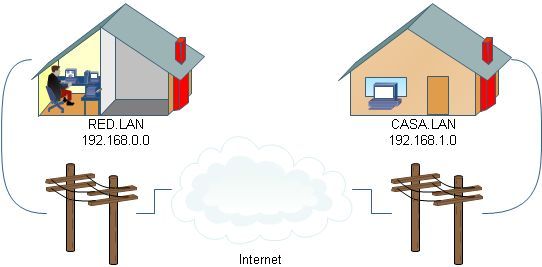
\includegraphics{imagenes/general/vpn_general_casas}
	\caption{Conexi�n a nivel exterior de una VPN entre dos redes dom�sticas.}
	\label{fig:diagrama_general_vpn}
\end{figure}

\subsection{Observaciones}

Uno de los motivos por lo que se ha extendido la utilizaci�n de VPN en las empresas es la facilidad de poner en pr�ctica una soluci�n estable, segura y en relativamente poco tiempo. Por esta raz�n es que en vez de alquilar un enlace WAN dedicado, es m�s conveniente econ�micamente (quiz�s en seguridad y prestaciones) establecer enlaces de tipo VPN entre los extremos, siempre que ambos est�n conectado a Internet.

Con respecto a las desventajas en materia de seguridad tanto en una l�nea dedicada como en una VPN, las fallas puede provenir no solo de las imperfecciones de la implementaci�n, sino de la interacci�n humana en el enlace, tanto en una como en otra. Por ejemplo, una l�nea dedicada puede parecer m�s segura por tener un �nico enlace punto a punto, pero tambi�n pueden ocurrir cortes de los cables a prop�sito perdiendo la conexi�n entre ambos extremos. En las VPN, un usuario malicioso puede interceptar las claves durante el proceso de autenticaci�n y luego hacerse pasar por el extremo de confianza, y as� establecer una conexi�n directa con el extremo de la VPN.

Por otro lado, existe el problema de los clientes m�viles, ya que si pierden su equipo, todos los datos de enlace con la VPN quedan vulnerables y a disposici�n del nuevo poseedor del equipo. De esta manera no sirve de nada la extrema seguridad que se implemente en el servidor VPN, ya que te�ricamente el usuario del equipo robado es un ``usuario de confianza''.

\subsection{Ventajas y desventajas}

Las VPN adem�s de tener muchas ventajas frente a otras alternativas, tambi�n tienen sus desventajas y a veces su implementaci�n no es la mejor elecci�n, e incluso ser�a perjudicial optar por ellas.

Se deben analizar cu�les son los puntos a favor y en contra que poseen. Las ventajas son las siguientes:

\begin{description}
	\item[Integridad, confidencialidad y seguridad de datos] Esto se garantiza mediante la autenticaci�n de usuarios y encriptaci�n de datos. Depende de cu�n seguras sean las claves y de la complejidad de los algoritmos de encriptaci�n.
	\item[Una VPN reduce costos y son sencillas de usar] Al utilizar un VPN no se invierte en infraestructura de red f�sica (si se utiliza Internet, por ejemplo), esto representa un ahorro de varios miles de d�lares en la conexi�n de puntos muy distantes.
	\item[Facilita la comunicaci�n entre dos usuarios en lugares distantes] Un usuario en Par�s conectado a una VPN de Canad�, puede ver los recursos de la red a la que se conecta como si se encontrara en la misma red local, es decir, las VPN son transparentes a los usuarios finales.
\end{description}

Las desventajas son las siguientes:

\begin{description}
	\item[Tiempo de respuesta no garantizado] Si bien los hosts de una VPN \emph{creen} que se encuentran en una misma red local, el tiempo de respuesta depende de la red sobre la que se estableci� la conexi�n; en el caso de Internet, y en los horarios pico de uso, el tiempo de respuesta puede ser muy superior al deseado, haci�ndose dif�cil el uso de aplicaciones cr�ticas.
	\item[Confiabilidad del enlace] Una VPN, se establece sobre la infraestructura de otra red, por ejemplo Internet; esto hace que nuestra conexi�n dependa de la estabilidad de los nodos involucrados en las rutas que comunican nuestros hosts. Por ende, puede perderse la conexi�n, cuando los puntos intermedios se caen.
	\item[Seguridad] Si bien los protocolos que se utilizan para el establecimiento de las VPN son muy seguros, tienen sus puntos d�biles; si un usuario mal intencionado los encuentra podr�a llegar a violar la privacidad de la comunicaci�n.
\end{description}

\section{Topolog�as de las VPN}
\label{sec:topologias_vpn}

Las topolog�as de las VPN se derivan unas de otras e incluso pueden estar combinadas. Las tres m�s generales dependen de la manera en que se conectan los usuarios, que son:

\begin{itemize}
	\item Conexi�n host a host (m�quina a m�quina).
	\item Conexi�n host a red (m�quina a red).
	\item Conexi�n red a red.
\end{itemize}

\subsection{VPN Host a Host}

Es el modo de conexi�n m�s b�sico. Involucra �nicamente a dos hosts: uno act�a como servidor y el otro como cliente VPN (figura \ref{fig:conexion_host_a_host}).

\begin{figure}[htbp]
	\centering
		
\includegraphics{imagenes/general/host_a_host}
	\caption{Ejemplo de conexi�n VPN host a host.}
	\label{fig:conexion_host_a_host}
\end{figure}

Por un lado se puede pensar que esta topolog�a es innecesaria, ya que est� incluida en las otras topolog�as que se describen a continuaci�n; pero por otra parte, esta topolog�a, al igual que las otras, sigue siendo una soluci�n v�lida. Por ejemplo en una empresa que posee dos redes conectadas a trav�s de Internet; que no se trafican datos cr�ticos entre ambas, pero que cada cierto tiempo se debe sincronizar informaci�n de valor entre dos servidores, uno en cada red. Para esta situaci�n es conveniente establecer un enlace VPN temporal de tipo host a host. Pero si no se tomara alguna medida de seguridad para realizar este trabajo, se estar�a exponiendo los servidores a ser espiados por cualquiera que sea capaz de interceptar los datos. Por otro lado, configurar una VPN red a red ser�a demasiado complejo para este fin, debido a que el tr�fico en general no tiene importancia y solo se requiere un tiempo corto para transmitir de un servidor a otro, por lo tanto, la mejor soluci�n para estos casos es una VPN \emph{Host a Host} que se establece entre los servidores solo en el momento de la sincronizaci�n.

\subsection{VPN Host a Red}

En empresas de cualquier tama�o, casi siempre existen usuarios m�viles, es decir, empleados que salen de las oficinas (o que trabajan desde su casa), pero que necesitan estar conectados a la red de la compa��a. Igual que para el caso anterior, se sabe que no es una buena idea permitir el acceso a cualquier usuario o compartir informaci�n sin protecci�n (sin cifrado). La figura \ref{fig:conexion_host_a_red} muestra un esquema simplificado de este tipo de conexi�n.

\begin{figure}[htbp]
	\centering
		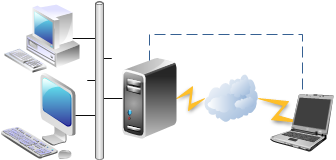
\includegraphics{imagenes/general/host_a_red}
	\caption{Ejemplo de conexi�n VPN host a red.}
	\label{fig:conexion_host_a_red}
\end{figure}

La implementaci�n de una VPN \emph{Host a Red} es una soluci�n segura para este tipo de situaciones, ya que posee la ventaja de que todo el tr�fico que circula a trav�s de ella est� encriptado; otro punto a favor de las VPN, es que el host remoto percibir� como si se encontrara dentro de la red local, pudiendo utilizar las direcciones IP privadas de la misma para interactuar con cualquier host de la red, impresora o dispositivo compartido de la red.

\subsection{VPN Red a Red}

Cuando se requiere asegurar el tr�fico a trav�s de Internet entre dos redes locales distantes, por ejemplo entre una sucursal y la casa central de una empresa, una VPN \emph{Red a Red} es una soluci�n disponible. La figura \ref{fig:conexion_red_a_red} muestra un esquema de este tipo de conexi�n.

\begin{figure}[htbp]
	\centering
		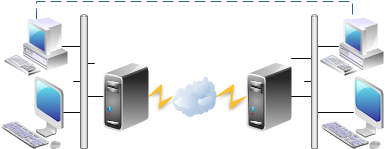
\includegraphics{imagenes/general/red_a_red}
	\caption{Ejemplo de conexi�n VPN red a red.}
	\label{fig:conexion_red_a_red}
\end{figure}

La conexi�n se establece entre los servidores VPN de cada red, dichos servidores son los que negocian todos los par�metros asociados a la VPN, haci�ndose totalmente transparente a los hosts internos de cada una; tanto es as�, que no es necesario reemplazar el software instalado en los equipos, ni configurar de manera especial (esta transparencia vale tambi�n para las otras topolog�as).

\section{Interacci�n con el Firewall}
\label{sec:interaccion_con_el_firewall}

En casi toda red de computadoras, existe un firewall; esto es un equipo (dedicado o no), cuya tarea es bloquear o permitir el tr�fico de paquetes desde o hacia Internet, u otra red vecina.

Es importante que el firewall de la red ``sepa'' reconocer el tr�fico VPN de los dem�s, ya que un error en la configuraci�n del mismo, puede dar lugar a que personas mal intencionadas ingresen a la red privada.

Vale aclarar que es necesario un servidor VPN solo en los casos de implementaci�n de topolog�as red a red, o host a red. Para las VPN host a host, deber�n crearse reglas expl�citas en el firewall que controlen el tr�fico de las conexiones, pero la funci�n de servidor la cumple uno de los dos hosts involucrados en la VPN. Sobre este tema, v�ase la Secci�n \ref{sec:topologias_vpn} en este mismo cap�tulo.

Para el trabajo en conjunto de una VPN con el firewall, se han encontrado tres maneras de interactuar:

\begin{itemize}
	\item VPN y firewall en el mismo equipo.
	\item VPN en paralelo con el firewall.
	\item VPN detr�s del firewall.
\end{itemize}

\subsection{Servidor VPN y Firewall en el mismo equipo}

Esta opci�n consta de un solo equipo en el cual conviven el firewall y servidor VPN, es decir, por este pasa el tr�fico directo a Internet (sin encriptaci�n), y el de las conexiones VPN (con cifrado). Este equipo debe tener dos tarjetas de red, una conectada a la red local, y la otra hacia Internet (u otra subred), como se muestra en la Figura \ref{fig:vpn_firewall_1}.

\begin{figure}[htbp]
	\centering
		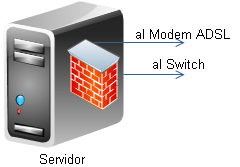
\includegraphics{imagenes/general/vpn_firewall_1}
	\caption{Servidor VPN y Firewall en un mismo equipo.}
	\label{fig:vpn_firewall_1}
\end{figure}

Las ventajas de esta soluci�n se listan a continuaci�n:

\begin{itemize}
	\item Al tener todo en un solo equipo, se simplifica el mantenimiento, ya que todo est� centralizado en �l.
	\item Se pueden crear reglas con el firewall, que se apliquen solo al tr�fico de la VPN, con las mismas herramientas que se utilizan para el tr�fico de Internet.
\end{itemize}

Las desventajas son las siguientes:

\begin{itemize}
	\item Se tiene solo un punto que controla toda la seguridad de la red; se debe tener la certeza que est� bien configurado, ya que cualquier falla puede dejar una puerta abierta a personas mal intencionadas.
	\item El tr�fico normal de Internet y el de VPN competir�n por los recursos del equipo, por lo que es posible que en este caso, sea necesario un equipo m�s potente.
\end{itemize}

\subsection{Servidor VPN en paralelo con el Firewall}

Ciertos firewalls no reconocen otros protocolos que no sean los de la suite TCP/IP. Cuando se implemente la VPN es necesario nuevos protocolos, por ejemplo \gls{GRE}, protocolo de transporte para VPNs con PPTP.

Al tener un firewall ya implementado en el sistema, de manera que no se pueda modificar (ya sea por las dificultades que presenta, o porque se ha adquirido alg�n producto comercial sin posibilidades de ampliar servicios), puede que esta sea una buena opci�n para no tener que cambiar todos los equipos.

Con respecto al ruteo, cada host dirige su tr�fico; si es directo a Internet pasa a trav�s del firewall, si es a una conexi�n VPN, pasa a trav�s del servidor VPN. No conviene la configuraci�n de rutas est�ticas en los hosts cuando estos son numerosos (o hay posibilidad de que lo sean), ya que es un trabajo tedioso y muy sujeto a errores humanos.

Las posibilidades m�s simples son, establecer en el firewall las rutas hacia el servidor VPN, de modo que cualquier paquete VPN que llegue al firewall, este lo redirigir� al lugar correcto; tambi�n es posible conectar un router entre el firewall y el servidor VPN, de modo que todos los paquetes se dirijan al router y este los env�e al sitio correcto. Un esquema ilustrativo de esta situaci�n, puede verse en la Figura \ref{fig:vpn_firewall_2}.

\begin{figure}[htbp]
	\centering
		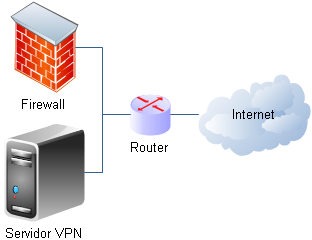
\includegraphics{imagenes/general/vpn_firewall_2}
	\caption{Servidor VPN y Firewall en equipos diferentes.}
	\label{fig:vpn_firewall_2}
\end{figure}

Con cualquiera de estas dos posibilidades, en los hosts basta configurar la puerta de enlace predeterminada. Las ventajas de este modo de conexi�n son:

\begin{itemize}
	\item Con este esquema los flujos de paquetes de las VPN no compiten por recursos del mismo equipo con el resto del tr�fico, con lo que se gana rendimiento.
	\item Se obtiene mayor escalabilidad, ya que si se requiere agregar m�s servidores VPN para repartir la carga de las conexiones, solo se deben conectar en paralelo con los equipos ya instalados.
\end{itemize}

Las desventajas de este m�todo de conexi�n pueden ser las siguientes:

\begin{itemize}
	\item Ahora existen dos puntos conectados al router de salida, por lo que aumenta la carga en cuanto al mantenimiento e inspecci�n de seguridad. Ahora se tienen que controlar dos o mas equipos.
	\item Aumentan los costes en gastos de equipos y el mantenimiento de los mismos.
\end{itemize}

\subsection{Servidor VPN detr�s del Firewall}

Se pueden centralizar las entradas y salidas a Internet solamente a trav�s del firewall, para ganar en seguridad y simplificar el mantenimiento, conectando el servidor VPN directo a la LAN y directo al firewall. Esto �ltimo puede hacerse con un cable cruzado para evitar el retardo normal de un switch. Esto se puede observar en la Figura \ref{fig:vpn_firewall_3}.

\begin{figure}[htbp]
	\centering
		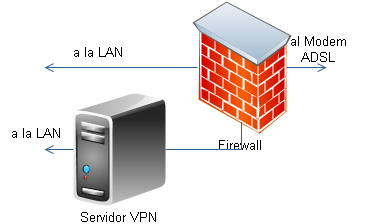
\includegraphics{imagenes/general/vpn_firewall_3}
	\caption{Servidor VPN detr�s del Firewall.}
	\label{fig:vpn_firewall_3}
\end{figure}

Respecto al ruteo, se debe hacer lo mismo que para el \emph{servidor VPN en paralelo con el Firewall}. Las ventajas que pueden mencionarse son las siguientes:

\begin{itemize}
	\item Se tiene solo un punto de flujo de paquetes desde y hacia la red local, por lo que se simplifica el mantenimiento.
	\item Las restricciones del tr�fico VPN est�n ubicadas �nicamente en el servidor VPN.
	\item Se gana en seguridad para la VPN, ya que el servidor no est� conectado directamente a Internet.
\end{itemize}

Las desventajas son:

\begin{itemize}
	\item Todo el tr�fico VPN debe pasar por el firewall, lo que introduce cierta latencia en las comunicaciones.
	\item El firewall debe soportar protocolos distintos a los de la suite TCP/IP, ya que los paquetes VPN circulan encapsulados con, por ejemplo, el protocolo GRE, en una VPN PPTP.
\end{itemize}

\section{Justificaci�n de las VPN}
\label{sec:justificacion_vpn}

En esta secci�n se tienen en cuenta aspectos que llevan a tomar la importante decisi�n de implementar o no un VPN en la empresa.

Resulta imprescindible tener en cuenta el aspecto econ�mico, ya que cuanto menos costosa la implementaci�n, m�s viable resulta el proyecto. Tambi�n se tienen en cuenta los aspectos de seguridad, ya que siempre es necesario transmitir datos confidenciales que requieren especial cuidado para que no caigan en manos no autorizadas.

Finalmente se debe tener en cuenta que la implementaci�n de una VPN no deber�a cambiar la infraestructura de la empresa, ni el modo de trabajar de los usuarios. Por eso es necesario que la instalaci�n y uso de la misma sea transparente a los usuarios.

\subsection{Econ�mico}

Una VPN es el modo barato de conectar dos redes (que pueden estar distantes) y de forma segura. Suponiendo que una empresa quiera unir sus oficinas de Argentina y Espa�a, en una sola ``Gran Red'', unas l�neas alquiladas o un enlace satelital supondr�an varios miles de d�lares tanto para la implementaci�n, como para el mantenimiento de los mismos; algo muchas veces dif�cil de justificar, y afrontar para las empresas.

La configuraci�n de una VPN, ser�a la soluci�n m�s econ�mica en este caso, ya que el gasto es significativamente menor en infraestructura, mantenimiento y capacitaci�n del personal.

\subsection{Seguridad}

Si bien es cierto que datos confidenciales de nuestra empresa pueden estar viajando, en el caso de una VPN, a trav�s de la red p�blica, estos son cifrados en el origen con algoritmos muy complejos, de modo que puedan ser des-cifrados �nicamente por el destino deseado.

Una VPN permite asegurar de una sola vez distintos protocolos: HTTP, POP3, SMB, etc. Lo cual representa una gran ventaja en tiempo y dinero, ante la idea de asegurar cada protocolo por separado.

Vale aclarar que las VPN, no aseguran todo el tr�fico hacia Internet, sino solo el que fluye a trav�s de ella.

\subsection{Transparencia}

La implementaci�n de una nueva tecnolog�a, trae como consecuencia, una gran resistencia por parte de los empleados que se ven obligados a utilizarla.

No es este el caso de las VPN, ya que es transparente a los usuarios. Continuando con el ejemplo visto anteriormente, al unir las oficinas de Argentina y Espa�a, los empleados percibir�n como si se encontraran en una misma red.
 
Se puede decir entonces, que la implementaci�n de la VPN, no requiere nuevos conocimientos por parte de la mayor�a de los usuarios de la misma. Otra ventaja es que no se necesita reemplazar el software que se est� utilizando.

\section{Consideraciones importantes}
\label{sec:intro_consideraciones_importantes}

En esta secci�n se van a plantear las diferentes tecnolog�as que en un tiempo fueron competidores directos de las VPN, aunque mucho antes de que �stas existieran, eran las �nicas opciones para asegurar dos o m�s redes.

Tambi�n se mencionar� la importancia de planificar un buen dise�o de la VPN para no comprometer la seguridad de la empresa, y adem�s, de algunos aspectos de administraci�n de las claves.

Por �ltimo se listar�n los casos en que la implementaci�n de una VPN se considera una buena opci�n y en los que pueden ser una verdadera p�rdida de tiempo.

\subsection{Comparaci�n con otras tecnolog�as}

Las VPN se pueden comparan con tecnolog�as \gls{RAS} y con las l�neas dedicadas. La primera permit�a a las personas trabajar desde su hogar y conectarse a la empresa por m�dem mediante marcado telef�nico por tonos. Esta tecnolog�a presentaba un problema de seguridad, que permit�a la conexi�n a cualquier persona que conociera el n�mero telef�nico del sistema, que luego fue resuelto mediante el sistema de \emph{re-llamada}. Otra limitaci�n de este sistema es su velocidad, que rondaba los 54 Kbps, y adem�s, por cada conexi�n se requer�a de un m�dem receptor. Por esta raz�n es que su implementaci�n resultaba muy costosa cuando se deb�a conectar un gran n�mero de clientes.

Las l�neas dedicadas pueden resultar recomendables en algunas aplicaciones. Por ejemplo si se tiene una base de datos que replica datos regularmente y que adem�s se realizan consultas constantemente y actualizaciones de forma intensiva, entonces se requiere del mayor ancho de banda posible, lo cual se consigue con l�neas dedicadas o con tecnolog�as \gls{MPLS}.

Algunas empresas de telecomunicaciones ofrecen conectividad mediante \gls{FrameRelay}, cuyo cometido es la transmisi�n de informaci�n a alta velocidad entre puntos geogr�ficamente distantes, mediante una red de alta velocidad, con una m�xima seguridad y calidad. Esta conexi�n se realiza a trav�s de circuitos virtuales permanentes (PVC), con ancho de banda bajo demanda y con un \emph{throughput} garantizado que permite alcanzar la velocidad convenida, que va de los 64 Kbps hasta los 2 Mbps, dependiendo del \emph{carrier}.

Esta tecnolog�a soporta cualquier aplicaci�n que requiera alto grado de conectividad tipo malla o tr�fico de datos tipo r�faga, con caracter�sticas de bajo retardo y calidad de servicio incluida. En este apartado, cabe aclarar, que mediante la conexi�n a Internet no se consigue calidad de servicio como lo permiten las l�neas dedicadas.

Otra de las tecnolog�as que utilizan los ISP para interconectar sitios de una empresa, es la recientemente mencionada MPLS, que dispone (seg�n el plan de contrato) de velocidades hasta 1 Gbps. Adem�s el servicio se encuentra subdividido de acuerdo a lo cr�tico que sea la transmisi�n, tanto para aplicaciones en tiempo real, de misi�n cr�tica o est�ndar. Por su parte, esta tecnolog�a es un poco m�s econ�mica que las l�neas dedicadas, pero a�n as� mucho m�s costosa que una soluci�n VPN propuesta en este trabajo.

Una desventaja importante de las l�neas dedicadas, es su elevado costo. Una instalaci�n completa por a�o puede llegar a valer unos 40000 d�lares; sin contar los costos de mantenimiento. En definitiva, este es un gasto casi imposible de afrontar por una empresa mediana o en crecimiento, por lo que esta soluci�n para unir dos redes de la empresa no es viable.

De esta manera, se han dado los cr�ditos a la implementaci�n de una VPN con software libre, que permite la transmisi�n de datos de manera segura (como el caso de Frame Relay o MPLS) y a bajo costo. Por ejemplo, el primer a�o de implementaci�n y funcionamiento de una VPN puede llegar a costar unos 6000 d�lares, que incluye un enlace punto a punto, soporte a clientes m�viles y mantenimiento mensual moderado (ver m�s detalles en \ref{subsec:comparativa_costos}), limit�ndose los a�os siguientes solamente a costos administrativos. Adem�s no ser�a necesario invertir en otras l�neas dedicadas (en caso de querer unir otras redes), ni en migraciones o en escalabilidad.

A pesar de ello, las grandes empresas optan generalmente por soluciones heterog�neas, donde en algunas aplicaciones y sectores se pueden implementar VPN con software libre, mientras que en otras �reas m�s cr�ticas, se utilizan soluciones comerciales como l�neas dedicadas, MPLS o VPN con hardware propietario.

\subsection{Planificaci�n de seguridad}

Para que las VPN funcionen bien dependen de muchos factores, no solo de la elecci�n del mejor cifrado ni el firewall m�s robusto y seguro que existe\footnote{Es necesario aclarar que, en realidad, no existe el mejor cifrado ni firewall.}. Si no se planifica cuidadosamente el dise�o de una VPN, la red entera puede ser vulnerable a�n con la VPN en funcionamiento.

Para planificar se debe involucrar a toda la gente que tenga que ver con el funcionamiento del sistema y con los servicios que ya se estaban utilizando. Por eso se requiere una buena comunicaci�n entre las personas que trabajen implementando la VPN y adem�s se debe asegurar que los administradores de sistemas, de redes y base de datos revisen el dise�o.

Adem�s se debe tener documentada la red completa, y cualquier cambio que se realice para la implementaci�n de la VPN, debe ser tambi�n documentado. El dise�o es un aspecto clave antes de poner en pr�ctica el sistema, en donde tambi�n se incluyen aspectos como la estrategia de administraci�n de claves, los m�todos de cifrado utilizados, la pol�tica de seguridad del firewall, entre otros.

\subsection{Administraci�n de claves}

La estrategia de administraci�n de claves es un punto importante en la planificaci�n de una VPN para las empresas. Por ejemplo se deben tener en cuenta las claves que utiliza un usuario m�vil, ya que si su port�til es robada, dichas claves deber�an ser revocadas inmediatamente, para no comprometer a toda la red de la empresa.

En algunos casos se utilizan m�s de una clave, y hasta se generan claves cada cierto tiempo, de manera que si una clave es comprometida, autom�ticamente se negocie otra distinta. De esta manera se evitan algunos problemas de seguridad, pero para esto, se debe tener una planificaci�n rigurosa en cuanto a los m�todos de revocaci�n de claves y a otras fallas en la VPN.

Por otro lado, para asegurar la confidencialidad y autenticaci�n se deben generar las claves correctamente. Algunos sistemas criptogr�ficos son vulnerables a ataques de an�lisis criptogr�fico porque las claves no se han generado de forma que sean seguras y no f�cilmente discernibles. En este caso se utiliza \gls{OpenSSL} para la generaci�n de las claves.

En ambos extremos de una VPN se necesitan claves para cifrar y descifrar, que deben ser transmitidas entre los sitios de forma segura. Se pueden hacer manualmente o mediante mecanismos de privacidad como \gls{PGP}. Si la VPN utiliza clave p�blica, se requieren dos pares de claves, por lo que se necesitar�a de un tercero de confianza para generar las claves. Este tercero puede no resultar un medio fiable para confiar la VPN, por lo que dicha parte debe tambi�n tener una buena pol�tica de seguridad para evitar estos problemas de confianza.

\subsection{Motivos de requerir una VPN}

En algunos casos, utilizar un VPN puede resultar la mejor opci�n, mientras que en otros ser�a una p�rdida de tiempo y dinero. En el siguiente listado se resume en qu� casos el uso de una VPN es la mejor opci�n:

\begin{itemize}
	\item Asegurar un cierto n�mero de recursos e informaci�n que atraviesan varias redes.
	\item Hacer que todos los host parecieran estar en una misma red, aunque se encuentren a kil�metros de distancia.
	\item Si se cuenta con usuarios m�viles que requieren tener acceso transparente a la red de la empresa.
	\item Se requiere administrar los servidores de forma remota por un canal seguro.
\end{itemize}

Estos casos que requieren de una VPN, hacen que una empresa separada f�sicamente, pueda tener una infraestructura de red segura, pero sin perder interacci�n con los clientes y usuarios m�viles. En este caso, una VPN puede asegurar todos los servicios que se utilicen en la empresa.

Por otro lado, si lo que se requiere es solamente asegurar ciertos protocolos o servicios entre un par de hosts, la implementaci�n de una VPN requerir�a un gran esfuerzo para un problema simple. Por eso para asegurar dos hosts basta con utilizar software de tunelado de un puerto a otro a trav�s de un canal cifrado y autenticado como \gls{SSH}.


%% Realizaci�n del proyecto
%%%%%%%%%%%%%%%%%%%%%%%%%%%%%%%%%%%%%%%%%%%%%%%%%%%%%%%%
%   |-------------------------|                        %
%   |REDES PRIVADAS VIRTUALES |                        %
%   |                         |                        %
%   | Proyecto de graduaci�n  |                        %
%   |_________________________|                        %
%                                                      %
%   Autores                                            %
%   -------                                            %
%                                                      %
% * Formoso Requena, Nicol�s Federico (CX02-0239-8)    %
%     nicolasformoso@gmail.com                         %
% * Cortez, Gustavo Maximiliano (CX01-0801-9)          %
%     cmgustavo83@gmail.com                            %
%                                                      %
%   Tutores                                            %
%   -------                                            %
%                                                      %
% * Ing. Gustavo Vanetta - vanettag@gmail.com          %
% * Lic. Miguel Bazzano - miguelbazzano@gmail.com      %
%                                                      %
%%%%%%%%%%%%%%%%%%%%%%%%%%%%%%%%%%%%%%%%%%%%%%%%%%%%%%%%

% ********* Realizaci�n del proyecto ********** %

\chapter{Realizaci�n del proyecto}
\label{chap:RealizacionDelProyecto}

En este cap�tulo se describen los objetivos y los pasos a seguir durante la investigaci�n, documentaci�n y evaluaci�n de las diferentes soluciones VPN.

Adem�s se especifica el alcance del proyecto, tanto en la pr�ctica como en los fundamentos te�ricos que se van a incluir.

\section{Objetivos}
\label{sec:realizacion_objetivos}

Los objetivos planteados para la tesis de investigaci�n e implementaci�n \textsc{Redes Privadas Virtuales} son los siguientes:

\begin{itemize}
	\item Definir una VPN (Virtual Private Network, o Red Privada Virtual en castellano), los tipos de conexiones y aplicaciones en la vida real.
	\item Presentar soluciones para la interconexi�n segura de computadoras y/o redes de computadoras, teniendo en cuenta el equilibrio entre los costos y beneficios en contraste a las alternativas comerciales.

	\item Detallar los m�todos actuales de conexi�n a Internet para empresas que pretendan tener su portal comercial siempre disponible en l�nea, junto a otros servicios dentro de la red local.

	\item Redactar los aspectos te�ricos y pr�cticos de las configuraciones VPN para concretar una transferencia de informaci�n segura, r�pida, privada y de confianza.

	\item Tener en cuenta que el dise�o e implementaci�n de las soluciones sean acordes a los est�ndares m�s utilizados en la actualidad, de manera que permitan el f�cil crecimiento de la infraestructura y as� tambi�n el mantenimiento de las redes.

	\item Requerir que el modo de conexi�n sea transparente al sistema operativo de las terminales de usuarios, por m�s que los servidores trabajen con sistemas diferentes.
\end{itemize}

\subsection{Especificaciones}

Se estudian las diversas topolog�as de comunicaci�n utilizando t�cnicas de VPN, que permiten el tr�fico de informaci�n asegurada y garantizada entre redes, terminales de usuarios o ambos entre s�. Para esto se utilizan herramientas de software libre como OpenVPN, \gls{ISAKMP}, PoPtoP, entre otros, que permiten la comunicaci�n entre dos puntos remotos utilizando la misma infraestructura de Internet bajo protocolos como \gls{IPSec}, \gls{PPTP}, etc. Adem�s las pruebas desde el lado del usuario consisten en la utilizaci�n de sistemas operativos propietarios y libres, por lo que se tiene en cuenta el soporte de varios servicios VPN, para evitar el cambio de par�metros o configuraciones en el momento de conectarse con un sistema operativo y luego con otro.

La conexi�n a Internet se realiza de tal manera que permita facilidad en el registro de conexiones, recursos y hasta en posibles problemas de seguridad. Para esto se utilizan Modem ADSL que se conectan al proveedor y a su vez el servidor \gls{OpenBSD} que provee acceso a los clientes de la red local. Este servidor se encarga de establecer la conexi�n propiamente dicha a Internet, de configurar los par�metros de seguridad y de ofrecer servicios adicionales como correo electr�nico con SendMail, DNS con Bind, DHCP con DHCP Server, Firewall con PF, repositorio de control de versiones con Subversion, terminal remota con OpenSSH, entre otros servicios. Por otro lado, para obtener un dominio fijo con direcciones IP din�micas se utilizan servicios como ZoneEdit, para automatizar los cambios de direcciones IP del proveedor manteniendo el nombre de dominio fijo y as� no se pierdan los enlaces VPN que dependen del dominio.

Finalmente se analiza el costo de implementaci�n en los servidores, que en cuanto a licencias de software se refiere, se tiene un gasto nulo; esto representa una gran ventaja si se lo compara con soluciones comerciales, las cuales van de los cientos a los miles de d�lares (en hardware, software y soportes t�cnico). Por otro lado, al utilizar una VPN bajo la infraestructura de Internet, no se invierte dinero en l�neas dedicadas, cuya instalaci�n y mantenimiento representa un gasto imposible de afrontar para muchas empresas e instituciones. La investigaci�n de las soluciones con software libre, van desde la instalaci�n del sistema operativo servidor hasta las pruebas de velocidad, seguridad y estabilidad de la red, pasando por la configuraci�n de conexi�n de banda ancha, configuraci�n del Firewall y de las aplicaciones extras que se utilizan durante el proceso de autenticaci�n entre los sistemas remotos.

\subsection{Conceptos involucrados}

Las materias relacionadas con el tema de esta tesis se podr�an resumir de la siguiente manera:

\begin{itemize}
	\item Redes de �rea Local
	\item Redes de �rea Extendida
	\item Protocolo de Comunicaci�n TCP/IP 
	\item Sistemas Operativos 
	\item Seguridad y encriptaci�n
\end{itemize}

\section{Proceso de desarrollo}
\label{sec:proceso_de_desarrollo}

La Figura \ref{fig:proceso_desarrollo} muestra de forma generalizada el proceso que se lleva a cabo para la realizaci�n de esta tesis. Para comenzar, se hicieron propuestas de los temas que se pod�an incluir e investigar. Luego se evaluaban si se pod�an realizar y finalmente quedaban como propuestas v�lidas para incluirlas en el proyecto.

\begin{figure}[htbp]
	\centering
		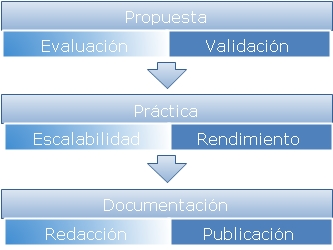
\includegraphics{imagenes/general/proceso_desarrollo}
	\caption{Diagrama del proceso de desarrollo de la tesis.}
	\label{fig:proceso_desarrollo}
\end{figure}

El siguiente paso es la puesta en pr�ctica de la propuesta, en la que se tiene en cuenta la posibilidad de escalabilidad de la soluci�n y adem�s se mide el rendimiento para comprobar si es aceptable o no para determinados fines.

Finalmente se documentan todos los detalles de las pruebas realizadas, teniendo en cuenta la redacci�n utilizada para referirse al lector. Para la presentaci�n del informe se utiliza el formato est�ndar PDF junto a las fuentes LaTeX del mismo.

\subsection{Alcance del proyecto}

El alcance del proyecto se define de acuerdo a las necesidades que surgen y a medida que se va avanzando en el tema. De esta manera, se comienza con casos sencillos, evaluando el rendimiento y la m�xima utilidad posible en �mbitos empresariales, pasando por esquemas alternativos de conexi�n y terminando por esquemas tan complejos como seguros y �ptimos para entornos de gran cantidad de conexiones simult�neas\footnote{Debido a las limitaciones econ�micas, no es posible recrear un ambiente real para llevar al l�mite la investigaci�n, por esta raz�n se ha hecho de experiencias ajenas para validar los resultados.}.

Adem�s se tienen en cuenta aspectos como la configuraci�n de la conexi�n a Internet de las redes locales, que m�s tarde establecen un enlace VPN entre las mismas simulando una gran red separadas por la nube de Internet.

\subsection{Limitaciones t�cnicas}

Para no entrar en demasiados detalles de los protocolo utilizados (dado que alguno de ellos puede llegar a ser tan complejo como el mismo \gls{IPSec}), se realizan breves descripciones de los mismos, tales como su origen, funcionamiento, ventajas y desventajas, entre otros fundamentos. No se describen detalles como los elementos de las tramas (n�meros de bits) o el trabajo que se realiza a bajo nivel (o nivel del kernel), sino que se rescatan los puntos importantes que pueden ser manejados por el administrador de la VPN o de la red en el espacio de usuario.

Otra limitaci�n del proyecto, que se encuentra fuera del alcance t�cnico propio, es el ancho de banda de la conexi�n a Internet (establecida por el proveedor de acceso o ISP en el momento de adquirir el servicio)\footnote{En este caso, se cuenta con 1 Mbps para bajada de datos y 256 Kbps para la subida.}. Adem�s, las pruebas que se realizan, generalmente son efectuadas en rangos horarios de bajo tr�fico de datos, que pueden ser en horarios matutinos o diurnos.

En cuanto a las pruebas realizadas, las limitaciones se basan en la cantidad de servicios que puedan ser instalados en los sistemas y probados por ambos extremos de la VPN, tales como sistemas de voz sobre IP (utilizando Asterisk), servicios de m�sica o radio en vivo (Icecast), servicios Web para todas las redes conectadas a la VPN, entre otros. Otra limitaci�n es la dificultad que presentan algunos servicios para su configuraci�n y puesta en marcha, ya sea porque no estan totalmente adaptados para funcionar en determinado sistemas o porque requieren de un alto nivel de conocimientos, que en definitiva, alejar�an al objetivo de este proyecto.

\subsection{Limitaciones econ�micas}

Algunos problemas que surgieron durante la configuraci�n de la conexi�n a Internet estaban m�s relacionados con la calidad de los dispositivos utilizados, o que no cumplen con lo especificado por el fabricante, como el caso del modem Aztech DSL600EW (Ap�ndice \ref{sec:descrip_red1}). Esto se debe al reducido costo de los materiales que se utilizan, produciendo un producto de baja calidad.

El uso de dispositivos dedicados (cajas negras) para establecer redes privadas virtuales, tiene un costo elevado y es justificable en entornos empresariales con gran cantidad de usuarios y conexiones.

El l�mite econ�mico se refiere a la dificultad en adquirir tanto hardware como software pre configurados para establecer una VPN con la m�nima intervenci�n del administrador. Se consideran tambi�n los equipos servidores y terminales que se pueden utilizar para simular conexiones m�ltiples, y todo lo que hace a la infraestructura de conexi�n a Internet en el hogar, como la implementaci�n en m�quinas virtuales antes de su instalaci�n en equipos reales.

\section{Entornos de evaluaci�n}
\label{sec:realizacion_entornos}

Los escenarios en que se realizaron las pruebas y evaluaciones no constituyen un ambiente empresarial, sino que se tratan de hogares de familia en los que se disponen generalmente de equipos modestos, no de supercomputadoras ni grandes servidores, sino simplemente equipos que se pueden adquirir por precios muy bajos. Los equipos utilizados se describen con m�s detalles en el Ap�ndice \ref{appendix:equipos_de_prueba}.

En esta secci�n se van a tratar los sistemas operativos utilizados para las conexiones y pruebas, adem�s de otras herramientas de software que permite comprobar y registrar las comunicaciones establecidas.

\subsection{Sistemas BSD}

La elecci�n de OpenBSD como sistema principal para proveer acceso a Internet no se basa en un an�lisis riguroso de costo y rendimiento, sino m�s bien en la posibilidad de utilizar un sistema gratuito, robusto y que puede ejecutarse en equipos antiguos.

Existen muchas variantes de sistemas BSD, cada una orientada a determinado tipo de usuarios y funcionalidades. Por ejemplo FreeBSD esta m�s orientado a usuarios de escritorio como intenta ser cualquier distribuci�n de Linux.

En las siguientes secciones se describir�n brevemente cada uno de estos sistemas, con el fin de concluir el motivo de la elecci�n de OpenBSD como servidor de Internet.

\subsubsection{FreeBSD}

La idea de FreeBSD es producir un sistema operativo utilizable para cualquier prop�sito, como Ubuntu, Tuquito, Fedora, SuSE, es decir, un sistema de prop�sitos generales. Se intenta que sea f�cil de usar y contenga una gran cantidad de paquetes (programas) para instalar.

\subsubsection{OpenBSD}

OpenBSD esta orientado a la seguridad m�s que nada. Las pol�ticas de seguridad son muy estrictas en el desarrollo, ya que cada c�digo que incluyen son auditados exaustivamente para corregir la mayor cantidad de bugs\footnote{Se le llaman bugs a los errores que se encuentran en sistemas de software, cuando se realiza una determinada operaci�n.} posibles.

\subsubsection{NetBSD}

NetBSD esta dise�ado como sistema operativo que puede ser distribuido gratuitamente a profesionales, entusiastas e investigadores, para que lo usen como quieran. El objetivo principal de este sistema es la portabilidad a trav�s de la mayor cantidad de equipos, tanto de 32 como de 64 bits. Tambi�n acent�an la buena escritura del c�digo, la estabilidad y eficiencia del sistema.

\subsection{Caracter�sticas de OpenBSD}

El proyecto OpenBSD es un sistema operativo libre tipo Unix, multiplataforma, basado en 4.4BSD. Los esfuerzos de desarrollo se concentran en la portabilidad, cumplimiento de normas y regulaciones, correcci�n del c�digo, seguridad proactiva y criptograf�a integrada.

A continuaci�n se exponen algunas razones por las que OpenBSD es un sistema operativo de gran utilidad para la realizaci�n de este proyecto:

\begin{itemize}
	\item Es reconocido por profesionales de la seguridad inform�tica como el sistema operativo tipo UNIX m�s seguro; esto es el resultado de una intensa e interminable auditor�a de seguridad sobre el c�digo fuente.
	\item Es un sistema operativo con todas las funcionalidades de UNIX que se puede adquirir de forma gratuita.
	\item Integra las �ltimas tecnolog�as en seguridad para la implementaci�n de cortafuegos (filtros de IP) y redes privadas virtuales (VPN) dentro de un entorno distribuido.
\end{itemize}

Estas son las caracter�sticas filos�ficas del sistemas; las caracter�sticas pr�cticas se dejaron de lado porque en el transcurso de esta tesis se van a describir detalladamente los puntos s�lidos del sistema. 

\subsection{Recomendaciones de instalaci�n}

Las recomendaciones para una instalaci�n limpia e inteligente se pueden enumerar a continuaci�n:

\begin{itemize}
	\item Bajar siempre la �ltima versi�n e instalarla en un disco vac�o.
	\item Realizar un particionado inteligente, aprovechando el espacio en disco y asegurando la raiz, evitando que usuarios malintencionados copen la unidad completa.
	\item Si se va a instalar un servidor, evitar compartir el sistema con otro sistema operativo
	\item Si se usa como servidor, no instalar el entorno gr�fico y mucho menos los grandes paquetes de KDE o Gnome
	\item Si se van a realizar pruebas, primero se debe intentarlo con una m�quina virtual
\end{itemize}

\subsection{Sistemas Linux}

Linux es un sistema operativo multitarea, multiusuario, multiplataforma y multiprocesador, desarrollado inicialmente por Linus Torvalds en el a�o 1991, y actualmente mantenido por una gran comunidad de usuarios y programadores.

Como la correcta definici�n y descripci�n de este sistema operativo no es el cometido de esta tesis, solamente se va a indicar que Linux en s�, se refiere al \gls{kernel} o n�cleo del sistema que es el que se encarga de la intercomunicaci�n entre el hardware del equipo y los programas de usuarios. Pero para que Linux sea un sistema operativo completo (con las herramientas necesarias para su administraci�n) se debe hacer uso de muchas aplicaciones que permitan su administraci�n y uso. Por esta raz�n, ha habido una controversia en el nombre de solo Linux, y la inclusi�n de GNU/Linux para referenciar a todo el sistema operativo. Aqu� se va a hacer referencia a Linux como si fuera todo el sistema operativo, pero si se requiere indicar otros componentes de \gls{GNU}, se har�n menci�n expl�citamente.

En cuanto a las distribuciones de Linux, hay una gran cantidad para casi todos los prop�sitos espec�ficos y de prop�sito general. Las m�s conocidas son Fedora, OpenSuSE, Ubuntu, Debian, Gentoo, entre otras.

Las empresas que trabajan con software libre idearon un modelo de negocios totalmente diferente al que se conoc�a hasta el momento, y es el de los servicios. En algunos casos, el producto se vende a un precio determinado (como RedHat o SuSE), mientras que en otros casos, las ganancias para las empresas radican en los servicios post venta (o post distribuci�n).

Para la realizaci�n de esta tesis se han utilizado distribuciones armadas de Linux, como Ubuntu Server, que es una versi�n orientada a servidores desarrollada por la empresa Canonical	Ltd., que encabeza el desarrollo de una de las distribuciones m�s utilizadas por su simplicidad y facilidad de uso.

Ubuntu Server en comparaci�n con la versi�n de escritorio del mismo fabricante, se caracteriza por la falta de entorno gr�fico, la optimizaci�n del sistema, la seguridad en los servicios, entre otros aspectos. Esto es principalmente, porque en un equipo servidor no es necesario un entorno gr�fico, ni el uso de procesos que hacen buena la experiencia del usuario, pero son totalmente in�tiles en servidores.

El sistema viene con configuraciones predeterminadas y servicios adicionales con la posibilidad de agregarlos durante la instalaci�n del sistema. Por ejemplo, los servicios que pueden agregarse en la instalaci�n son OpenSSH, para permitir el acceso remoto por \gls{SSH}, servidor Web, Samba (servidor de archivos), correo electr�nico (con TLS), entre otros.

La utilizaci�n de Linux ``Ubuntu Server'' como servidor VPN, es m�s por cuestiones pr�cticas que t�cnicas, ya que hoy en d�a casi cualquier distribuci�n de Linux cuenta con las mismas caracter�sticas y posibilidades de expansi�n. Vale aclarar que algunas distribuciones vienen mejor preparadas que otras para utilizarlas en servidores.

En particular, Ubuntu Server ha sido modificado para que funcione como servidor, consumiendo pocos recursos (solamente los necesarios), optimizando la seguridad del sistema y servicios como DNS, correo electr�nico, SSH, Samba, etc.

\subsection{Sistemas Windows}

El sistema operativo Windows es la denominaci�n de una familia de productos desarrollados por Microsoft tanto para uso de escritorio como para servidores. La primera versi�n fue liberada en el a�o 1985 y a partir de entonces se realizaron gran cantidad de modificaciones en el n�cleo y otros componentes como las implementaciones y soporte a dispositivos de red, impresoras, entre otros perif�ricos.

En la realizaci�n de esta tesis, se han utilizado dos versiones de Windows, XP y Vista. Ambas solo cumpl�an el papel de entornos de escritorio y en algunos casos se han utilizado las herramientas que vienen incluidas como el registro del sistema, la configuraci�n de conexiones entrantes y salientes, los comandos de ruteo y estad�sticas de la conexi�n.


%% Conexi�n a Internet
%%%%%%%%%%%%%%%%%%%%%%%%%%%%%%%%%%%%%%%%%%%%%%%%%%%%%%%%
%   |-------------------------|                        %
%   |REDES PRIVADAS VIRTUALES |                        %
%   |                         |                        %
%   | Proyecto de graduaci�n  |                        %
%   |_________________________|                        %
%                                                      %
%   Autores                                            %
%   -------                                            %
%                                                      %
% * Formoso Requena, Nicol�s Federico (CX02-0239-8)    %
%     nicolasformoso@gmail.com                         %
% * Cortez, Gustavo Maximiliano (CX01-0801-9)          %
%     cmgustavo83@gmail.com                            %
%                                                      %
%   Tutores                                            %
%   -------                                            %
%                                                      %
% * Ing. Gustavo Vanetta - vanettag@gmail.com          %
% * Lic. Miguel Bazzano - miguelbazzano@gmail.com      %
%                                                      %
%%%%%%%%%%%%%%%%%%%%%%%%%%%%%%%%%%%%%%%%%%%%%%%%%%%%%%%%

% *********** Cap�tulo: Conexi�n a Internet ********** %

\chapter{Conexi�n a Internet}
\label{chap:ConexionAInternet}

La conexi�n a Internet es un requisito muy importante en el mundo de los negocios de hoy en d�a, y como era de esperar, las VPN se mueven por esos �mbitos inseguros, creando canales de datos que solo pueden entender los extremos autorizados y asegurando la informaci�n. Es por eso que para la realizaci�n de esta tesis es importante contar con una buena conexi�n a Internet, aunque sea con el perfil de \emph{servidor hogare�o}, basta para lograr el objetivo de establecer una VPN.

En este cap�tulo se dar�n a conocer los detalles de la conexi�n a Internet de los equipos utilizados para las pruebas que requieran una conexi�n real para probar una VPN. En este caso se utilizar� el sistema operativo OpenBSD en el  servidor de acceso a Internet entre otros servicios adicionales.

Tambi�n se detallar�n los par�metros de configuraci�n del firewall y algunos aspectos a tener en cuenta para automatizar el proceso de inicio.

\section{Configuraci�n del servidor}
\label{sec:configuracion_servidor_hogar}

%REVISAR ESTOS PRIMEROS P�RRAFOS... VAN ???
%ME PARECE QUE NO VA, PORQUE NOSOTROS NO NECESITAMOS HABLAR DE LAS CONEXIONES EN HOGARES, SINO EN EMPRESAS.
Hace algunos a�os las necesidades de comunicaci�n en un hogar se limitaban al uso de la l�nea telef�nica (sea fija o m�vil), dejando de lado la conexi�n a Internet que en la mayor�a de los casos, se trataban de terminales que se conectaban a la red y no se compart�a el ancho de banda con otras computadoras, utilizando el limitado enlace telef�nico para la transferencia de datos.

Con la llegada de la banda ancha y el abaratamiento del hardware, las familias pod�an contar con m�s de una computadora personal, ya que vender la vieja PC, luego de comprar un equipo m�s potente, no generaba m�s ganancias de las que se podr�a aprovechar conect�ndola en red y compartiendo la costosa banda ancha que hab�a en aquella �poca. Pero a�n as�, no se dispon�a de una PC libre para que realizara la conexi�n, sino que se la usaba como una terminal de trabajo m�s.

Luego con la disminuci�n de precios de la banda ancha y de las PC, los usuarios hogare�os ya pod�an contar con peque�as redes dom�sticas en las que compartir documentos, m�sica, fotos y hasta la conexi�n a Internet por banda ancha, no resultaba muy costoso. Adem�s, se pod�a disponer de la PC m�s vieja como ``servidor'' de Internet. Por eso es que, compartir la conexi�n, ya no necesitaba depender de la PC principal (o la m�s ``grande'' o nueva) sino que se comenzaba a pensar en una pol�tica m�s inteligente para ofrecer servicio continuado y seguro a toda la familia. Esto es ni m�s ni menos que utilizar una PC de recursos moderados para que ofrezca servicios a toda la red interna con todas las ventajas que supone un sistema libre, seguro y flexible como OpenBSD.

\subsection{Planificaci�n}

A continuaci�n se detallan los pasos que se siguieron para dejar a punto el servidor OpenBSD de cada red. Como se ver� m�s adelante, este cumple funciones de servidor DHCP, DNS, Firewall, Conexi�n a Internet, entre otras cosas.

Al ser las nuestras redes de no m�s de cinco hosts, podemos darnos el lujo de poner todos los servicios en un solo ordenador. Pero en una empresa mediana, esto es irrealizable, ya que son necesarios servidores separados de casi todas estas cosas.

Los pasos para la instalaci�n y configuraci�n de nuestros servidores fueron: 

\begin{itemize}
	\item Instalaci�n base de OpenBSD,
	\item Configuraci�n de la conexi�n a Internet,
	\item Asociaci�n de un dominio propio,
	\item Configuraci�n de Packet Filter (firewall),
	\item Correo interno con SendMail,
	\item Servidor DHCP,
	\item Retoques en la configuraci�n general del sistema,
	\item Automatizaci�n del sistema de arranque,
	\item Utilizaci�n de algunas herramientas de red y del sistema.
\end{itemize}

El orden de estos pasos es cronol�gico, pero en algunos casos, el punto siguiente no depende del anterior. 

\subsection{Las Redes}

Ambas redes utilizan el protocolo TCP/IP para la comunicaci�n entre sus respectivos hosts, con IP versi�n 4 (IPv4); los rangos de direcciones ip privadas utilizados en las redes locales son: para la red 1 192.168.1.0, y para la red 2 192.168.0.0; la m�scara de red en ambos casos es la misma: 255.255.255.0.

En las dos redes hay solo una puerta de enlace a la red p�blica; dicha puerta establece una conexi�n PPPoE con el Proveedor de Servicios de Internet (o ISP). A trav�s de ellas se trafican todos los paquetes entre la red p�blica y cada una de las redes locales, y es por donde fluir�n los paquetes que pertenezcan a la conexi�n VPN.

Cada una de las redes cuenta con un firewall a la entrada, que en el caso de la red donde se encuentra el host que har� las veces de servidor VPN, dicho firewall deber� ser configurado apropiadamente, como se ve en los cap�tulos \ref{chap:proto_pptp} y \ref{chap:vpn_pppsobressh}. Un resumen de este esquema en un extremo de la red se muestra en la figura \ref{fig:conexion_directa_openbsd}.

\begin{figure}[htb]
	\begin{center}
	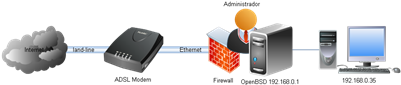
\includegraphics{imagenes/general/conexion_directa}
	\caption{Esquema de conexi�n directa de un equipo con el servidor OpenBSD.}
	\label{fig:conexion_directa_openbsd}
	\end{center}
\end{figure}

El primer elemento (desde la derecha) de la figura \ref{fig:conexion_directa_openbsd} es una PC con direcci�n IP 192.168.0.35 que ha sido asignada por el segundo elemento (la puerta de enlace OpenBSD con direcci�n 192.168.0.1) previamente configurado por el administrador del sistema para brindar servicios de DHCP sobre la interfaz de red correspondiente. El siguiente elemento es el firewall, este se encarga de filtrar el tr�fico no deseado que quiera ingresar a nuestra red local. Por �ltimo, el Modem ADSL realiza la conversi�n de interfaz que utiliza el servidor (Ethernet) hacia la l�nea telef�nica que previamente detecta el enlace con el proveedor y obtiene un enlace WAN a trav�s de la boca tipo RJ11 est�ndar de las l�neas de tel�fono.

En la secci�n \ref{sec:esquema_conexion} se ver� con m�s detalles el esquema de conexi�n de la red.

\section{Configuraci�n general del sistema}
\label{sec:configuracion_general_openbsd}

Suponiendo que se tiene instalado correctamente OpenBSD en el equipo servidor, solo resta configurar el sistema en general para poder realizar la conexi�n a Internet propiamente dicha.

Luego de conectar la placa de red libre a la interfaz ethernet del modem ADSL, se tiene que configurar el archivo /etc/hostname.if, donde ``if'' se reemplaza por la interfaz de red. Por ejemplo al ejecutar el comando \emph{ifconfig} se obtiene:

\begin{listing}[style=consola, numbers=none]
lo0: flags=8049<UP,LOOPBACK,RUNNING,MULTICAST> mtu 33208
        groups: lo
        inet 127.0.0.1 netmask 0xff000000
        inet6 ::1 prefixlen 128
        inet6 fe80::1%lo0 prefixlen 64 scopeid 0x5
rl0: flags=8843<UP,BROADCAST,RUNNING,SIMPLEX,MULTICAST> mtu 1500
        lladdr 00:08:54:b2:48:b6
        media: Ethernet autoselect (100baseTX full-duplex)
        status: active
        inet 192.168.0.1 netmask 0xffffff00 broadcast 192.168.0.255
        inet6 fe80::208:54ff:feb2:48b6%rl0 prefixlen 64 scopeid 0x1
ne1: flags=8863<UP,BROADCAST,NOTRAILERS,RUNNING,SIMPLEX,MULTICAST> mtu 1500
        lladdr 00:c0:df:ab:2e:f1
        media: Ethernet autoselect (10baseT full-duplex)
        inet6 fe80::2c0:dfff:feab:2ef1%ne1 prefixlen 64 scopeid 0x2
ne2: flags=8822<BROADCAST,NOTRAILERS,SIMPLEX,MULTICAST> mtu 1500
        lladdr 00:c0:df:ab:0b:e9
        media: Ethernet autoselect (10base2)
\end{listing}

La interfaz lo0 corresponde a loopback o interfaz local. Las dem�s interfaces son: rl0, ne1 y ne2; de las cuales, la primera se conecta al switch y tiene asignada una direcci�n IP (192.168.0.1); la segunda interfaz (ne1) esta conectada directamente al modem ADSL. La �ltima no esta conectada, pero podr�a utilizarse  para configurar zonas DMZ.

Para conectar la interfaz ne1 con el modem ADSL, en el archivo /etc/hostname.ne1 se escribe solamente:

\begin{verbatim}
up
\end{verbatim}

De esta manera se inicia la placa de red para ser utilizada con el Modem ADSL.

\subsection{Configuraci�n de PPP}

Para establecer la conexi�n se utiliza un protocolo de comunicaci�n punto a punto sobre ethernet (PPPoE). B�sicamente, lo que hace este protocolo, implementar la capa IP sobre el protocolo PPP, que es encapsulado en una trama ethernet y transmitida al ISP a trav�s de la l�nea telef�nica. Logrando de esta forma, transmitir paquetes IP por una conexi�n serial punto a punto establecida por dos puertos ethernet.

El archivo a modificar para realizar la conexi�n a Internet desde OpenBSD es \texttt{/etc/ppp/ppp.conf} que lleva todos los par�metros necesarios para la comunicaci�n, incluyendo el nombre de usuario y contrase�a, por lo que es muy recomendable que solamente pueda ser le�do por el administrador (root). Un ejemplo de configuraci�n se puede ver en el listado \ref{config:ppp.conf}.

\begin{configuracion}
\begin{listing}[style=configuracion]
default:
 set log Phase Chat LCP IPCP CCP tun command

proveedor:
 set redial 15 0
 set reconnect 15 10000
 set device "!/usr/sbin/pppoe -i ne1"
 set speed sync
 disable acfcomp protocomp
 deny acfcomp
 enable lqr
 set lqrperiod 5
 set dial
 set login
 set timeout 0
 set authname "nombre@arnet_o_cualquiera-tuc-xxx"
 set authkey "SuP3rP@sSw0rd"
 add! default HISADDR
\end{listing}
\caption{Ejemplo de configuraci�n de \texttt{ppp.conf}.}
\label{config:ppp.conf}
\end{configuracion}

Luego para realizar la conexi�n se ejecuta desde la l�nea de comandos lo siguiente:

\begin{listing}[style=consola, numbers=none]
$ sudo ppp -ddial proveedor
Working in ddial mode
Using interface: tun0
$
\end{listing}

Si al ejecutar \emph{sudo ppp -ddial proveedor} obtenemos la salida mostrada en el listado de arriba, significa que se ha creado la interfaz \emph{tun0} pero no que se haya conectado a�n. Para comprobar la conexi�n, se puede ver en los procesos del sistema con el comando ``px ax'' y localizar que los siguientes dos procesos aparezcan:

\begin{verbatim}
28682 ??  Is      0:00.23 ppp -ddial arnet
25835 ??  I       0:00.08 /usr/sbin/pppoe -i ne1
\end{verbatim}

Y para saber la direcci�n IP que ha asignado el proveedor, al ejecutar ``ifconfig'' nuevamente, se puede ver el nuevo dispositivo t�nel tun0 que ha creado PPP:

\begin{verbatim}
tun0: flags=8051<UP,POINTOPOINT,RUNNING,MULTICAST> mtu 1492
        groups: tun egress
        inet 190.137.64.32 --> 200.3.60.15 netmask 0xffffffff
\end{verbatim}

De esta manera, se asegura que la conexi�n a Internet se ha establecido y que la direcci�n IP asignada por el proveedor es \emph{190.137.64.32}. En la �ltima l�nea del archivo \texttt{ppp.conf} vemos que luego de establecer la conexi�n con el proveedor, se agreg� la ruta por defecto a la direcci�n del gateway del proveedor:

\begin{listing}[style=consola, numbers=none]
# route show -inet
Routing tables

Internet:
Destination        Gateway            Flags    Refs      Use    Mtu  Interface
default            200.3.60.15        UGS         2    11740      -   tun0
loopback           localhost          UGRS        0        0  33208   lo0
localhost          localhost          UH          1      120  33208   lo0
192.168.0/24       link#1             UC          2        0      -   rl0
superhijitus       00:08:54:b2:48:b6  UHLc        1      466      -   lo0
192.168.0.35       00:1e:90:22:26:1c  UHLc        1   166475      -   rl0
200.3.60.15        host32.190-137-64. UH          1        0   1492   tun0
BASE-ADDRESS.MCAST localhost          URS         0        0  33208   lo0
\end{listing}

Si en este momento se intenta obtener respuesta de alg�n dominio (por ejemplo con el comando ``ping google.com''), no se obtendr� respuesta alguna, pues todav�a se configur� el servidor DNS. OpenBSD se instala con un servidor de DNS preconfigurado y casi listo para usar con direcciones de Internet, se lo puede iniciar con el comando ``named'' y editar el archivo \emph{/etc/resolv.conf} como se indica en el listado \ref{config:resolv.conf}.

\begin{configuracion}
\begin{listing}[style=configuracion]
lookup file bind
search red.lan
nameserver 192.168.0.1
nameserver 200.45.191.35
\end{listing}
\caption{Servidor de nombre en \texttt{/etc/resolv.conf}.}
\label{config:resolv.conf}
\end{configuracion}

La primera l�nea (lookup) especifica d�nde buscar para resolver nombres. En este caso, busca primero en el archivo \texttt{/etc/hosts} y si no lo encuentra all�, utiliza el servidor DNS local y luego el remoto. A veces es buena pr�ctica agregar el DNS del proveedor por si a�n no se ha ejecutado o configurado Bind en el sistema.

Luego de esto, es posible acceder a Internet desde el servidor, pero a�n los dem�s equipos de la red no pueden hacerlo.

\subsection{Permitir el acceso a Internet}

Para permitir el acceso a Internet de los dem�s equipos de la red, a trav�s del servidor OpenBSD, se deben habilitar algunos par�metros del kernel; esto se hace con el archivo ``/etc/sysctl.conf''. Algunas l�neas de este archivo se muestran en el listado \ref{config:sysctl.conf}.

\begin{configuracion}
\begin{listing}[style=configuracion]
#       $OpenBSD: sysctl.conf,v 1.46 2008/01/05 18:38:37 mbalmer Exp $
#
# This file contains a list of sysctl options the user wants set at
# boot time.  See sysctl(3) and sysctl(8) for more information on
# the many available variables.
#
net.inet.ip.forwarding=1        # 1=Permit forwarding (routing) of IPv4 packets
#net.inet.ip.mforwarding=1      # 1=Permit forwarding (routing) of IPv4 multicast packets
#net.inet.ip.multipath=1        # 1=Enable IP multipath routing
net.inet6.ip6.forwarding=1      # 1=Permit forwarding (routing) of IPv6 packets
#net.inet6.ip6.mforwarding=1    # 1=Permit forwarding (routing) of IPv6 multicast packets
#net.inet6.ip6.multipath=1      # 1=Enable IPv6 multipath routing
#net.inet6.ip6.accept_rtadv=1   # 1=Permit IPv6 autoconf (forwarding must be 0)
#net.inet.tcp.rfc1323=0         # 0=Disable TCP RFC1323 extensions (for if tcp is slow)
#net.inet.tcp.rfc3390=0         # 0=Disable RFC3390 for TCP window increasing
net.inet.esp.enable=1           # 0=Disable the ESP IPsec protocol
net.inet.ah.enable=1            # 0=Disable the AH IPsec protocol
\end{listing}
\caption{Algunas l�neas de \texttt{/etc/sysctl.conf}.}
\label{config:sysctl.conf}
\end{configuracion}

Tal como se muestra en el listado anterior, las l�neas descomentadas (las que no tienen el s�mbolo \#) son las que lee el kernel para habilitar (si tiene un 1) o deshabilitar (si tiene un 0) al inicio del sistema.

Luego se debe activar el firewall Packet Filter del OpenBSD, en el archivo ``/etc/rc.conf'' para que se ejecute en el inicio del sistema. Tambi�n se pueden habilitar otros servicios �tiles tal como Bind. Una parte de este archivo de configuraci�n aparece en el listado \ref{config:rc.conf}.

\begin{configuracion}
\begin{listing}[style=configuracion]
#!/bin/sh -
#
#       $OpenBSD: rc.conf,v 1.128 2008/01/31 14:18:03 reyk Exp $

# set these to "NO" to turn them off.  otherwise, they're used as flags
sshd_flags=""           # for normal use: ""
named_flags=""          # for normal use: ""

# set the following to "YES" to turn them on
pf=YES                  # Packet filter / NAT
ipsec=YES               # IPsec
portmap=NO              # Note: inetd(8) rpc services need portmap too
inetd=YES               # almost always needed
check_quotas=YES        # NO may be desirable in some YP environments
accounting=NO           # process accounting (using /var/account/acct)
\end{listing}
\caption{Algunas l�neas de \texttt{/etc/rc.conf}.}
\label{config:rc.conf}
\end{configuracion}

S�lo resta configurar el PF para que realice las operaciones de NAT (traducci�n de direcciones de red), esto, para que los equipos de la red local puedan acceder a Internet con la IP p�blica asignada por el proveedor. Lo que se ver� con m�s detalles en la secci�n~\ref{sec:ReglasFiltradoOpenBSD}.

\section{Reglas de filtrado}
\label{sec:ReglasFiltradoOpenBSD}

A partir de la versi�n 3.0 de OpenBSD, luego de una disputa en la licencia utilizada en la implementaci�n del firewall, se comenz� el desarrollo de un nuevo software para que realizara las mismas y otras funciones m�s que el anterior. A esta implementaci�n se la ha denominado Packet Filter (abreviado como PF). 
  
PF es el programa que maneja un conjunto de instrucciones a nivel de kernel, que permite la gesti�n del tr�fico entrante y saliente del sistema. Adem�s realiza funciones de filtrado del tr�fico TCP/IP, NAT, control de ancho de banda y priorizaci�n de paquetes, entre otras cosas.

\subsection{Funcionamiento b�sico}

Cuando se habilita el sistema de filtrado de PF \textendash sea al arranque o manualmente\textendash\hspace{0.01cm} se carga el archivo ``/etc/pf.conf'', donde se configuraron las directivas del firewall, entre otras cosas. Este archivo es le�do y se carga en orden secuencial, de modo que existe dependencia entre las reglas. Dicho archivo consta de siete partes, y sigue un orden predeterminado como se enumera aqu�: 

\begin{enumerate}
	\item \textbf{Macros}: son las variables definidas por el usuario que pueden contener direcciones IP, nombres de hosts, interfaces de red, etc.
	\item \textbf{Tablas}: es una estructura que se usa para definir un conjunto de direcciones IP y puertos.  
	\item \textbf{Opciones}: son las opciones para el funcionamiento de PF.  
	\item \textbf{Normalizaci�n (Scrub)}: realiza el reprocesamiento de paquetes para su normalizaci�n y defragmentaci�n.  
	\item \textbf{Formaci�n de colas}: para proporcionar control de ancho de banda y priorizaci�n de paquetes.  
	\item \textbf{Traducci�n de direcciones}: controla la traducci�n de direcciones de red (NAT) y el redireccionamiento de paquetes.  
	\item \textbf{Reglas de filtrado}: permite el filtrado selectivo o el bloqueo de paquetes seg�n van pasando por las interfaces de red definidas. 
\end{enumerate}
  
Durante el procesamiento del archivo de PF es importante la ubicaci�n de las sentencias de bloqueo y apertura de puertos y protocolos, ya que si la l�nea que bloquea los puertos se encuentra despu�s de la l�nea que abre un conjunto de puertos determinados, PF entender� que la sentencia posterior es la que vale y anula la anterior, provocando un funcionamiento diferente al esperado (se supone abrir los puertos definidos). Por esto, a excepci�n de los macros y tablas, el archivo debe mantener el orden de los pasos anteriores. Tambi�n se puede obviar alg�n punto para una aplicaci�n espec�fica.

\subsubsection*{Anchors}

Una de tantas otras caracter�sticas que posee este firewall, es un concepto que se denomina \emph{anchor}. 

Un anchor es un contenedor dentro del cual se pueden agregar y quitar reglas de filtrado \emph{on the fly}, es decir, en tiempo de ejecuci�n. Con ellos, Se puede por ejemplo, agregar un conjunto de restricciones sin tener que recargar el PF completo.

Packet Filter da la posibilidad de anidar anchors, pudiendo luego ser invocados con la misma notaci�n que se utiliza en el filesystem de unix: separando los nombres de los anchors (de mayor a menor nivel) con una barra `/'.

Si se encuentra que un paquete corresponde con una regla que est� marcada con la opci�n \emph{quik}, dentro de un anchor, no se contin�a con las reglas subsiguientes, sino que se termina la evaluaci�n.

Un ejemplo de la utilizaci�n de anchors, puede verse en la secci�n~\ref{sec:isakmpd_fw}.

\subsection{Configuraci�n de Packet Filter}

Ahora un ejemplo de configuraci�n de Packet Filter para dejar salir a Internet a los equipos de una red local, se puede ver en el listado \ref{config:pf.conf_conexion_internet}.

\begin{configuracion}
\begin{listing}[style=configuracion]
# Interfaces de red
ext_if="tun0"
int_if="rl0"

# Politicas
set block-policy return
set loginterface $ext_if

# Normalizacion
scrub in all

# Ruteo, NAT y redireccionamiento
nat on $ext_if from $int_if:network to any -> ($ext_if)

# Reglas de filtrado
block all
pass quick on $int_if all
pass quick on lo0 all

# Permite el trafico desde la red interna
pass in  on $int_if from $int_if:network to any keep state
pass out on $int_if from any to $int_if:network keep state

# Permite salida de paquetes tcp, udp, icmp
pass out on $ext_if proto tcp all modulate state flags S/SA
pass out on $ext_if proto { udp, icmp } all keep state

# Responde a ICMP
pass in on $ext_if proto icmp all keep state
\end{listing}
\caption{Reglas de PF para permitir conexi�n a Internet.}
\label{config:pf.conf_conexion_internet}
\end{configuracion}

La interfaz interna (int\_if) no es m�s que la placa de red que ha detectado el sistema durante el arranque y est� conectada a la red local. En este caso se le ha asignado el nombre ``rl0''; este var�a de acuerdo al tipo de placa que se utilice (por ejemplo, para placas NE2000 o compatibles, se le asigna el dispositivo ``ne0'', ``ne1'' y as� sucesivamente).

Una vez cargados, estos par�metros de configuraci�n permiten la navegaci�n libre por Internet, con todos los puertos del servidor bloqueados. Para recargar las directivas del PF, ejecutamos lo siguiente: \emph{pfctl -f /etc/pf.conf}.

El firewall crea una interfaz para monitorear su funcionamiento, se la puede ver con el comando \emph{ifconfig}:

\begin{listing}[style=consola, numbers=none]
pflog0: flags=141<UP,RUNNING,PROMISC> mtu 33208
        groups: pflog
\end{listing}

Por ejemplo, para monitorear los mensajes que env�a PF ejecutamos el comando ``tcpdump -i pflog0''. 

\section{Esquema de conexi�n}
\label{sec:esquema_conexion}

Para dar acceso a Internet a una peque�a red local hogare�a, se utiliza un equipo con funciones de ruteo y firewall, cuyo esquema general se puede resumir en la figura \ref{fig:esquema_net_serv}.

\begin{figure}[htb]
	\begin{center}
	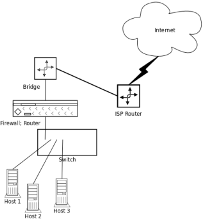
\includegraphics{imagenes/host-host/esquema_net_serv}
	\caption{Esquema de la red donde est� el servidor con OpenBSD.}
	\label{fig:esquema_net_serv}
	\end{center}
\end{figure}

Para conocer detalles de los hosts, v�ase el Ap�ndice \ref{appendix:equipos_de_prueba}. El equipo servidor de uno de los extremos de la conexi�n, funciona bajo OpenBSD y tiene instaladas tres placas de red; una de ellas se conecta a la interfaz Ethernet del Modem/Router ADSL. Esta �ltima, y la interfaz WAN de dicho router est�n configuradas como bridge; la otra se conecta con el Switch. Y la tercera se reserva para configurar zonas DMZ \footnote{Siglas de demilitarized zone o zona desmilitarizada.}.

%El Firewall tambi�n realiza funciones de ruteo, de NAT (???, me parece que esto no es as�)
El Firewall tambi�n realiza funciones de NAT (Network Address Translation), necesario para compartir el acceso a Internet con todos los hosts de la red local; el servidor tambi�n brinda servicios de DHCP, para la asignaci�n din�mica de direcciones. Adem�s se ha configurado un conjunto de reglas de filtrado para determinados puertos, direcciones IP y MAC, para evitar el uso del firewall cuando se realicen transferencias de datos dentro de la red local.
  
En este caso, como se trata de una red hogare�a, se permite el libre acceso hacia Internet, pero para establecer un nivel de seguridad adecuado, se bloquea cualquier conexi�n proveniente de Internet que no haya sido solicitada por un equipo que pertenezca a la red local.

En la figura \ref{fig:conexion_detallada_openbsd} se pueden ver con m�s detalles de los elementos que participan en la conexi�n a Internet, y tambi�n los dos PCs que comparten el acceso. Las mismas est�n conectadas a un switch que se encarga de ``repartir'' los datos entre los emisores y receptores de la red.

\begin{figure}[htb]
	\begin{center}
	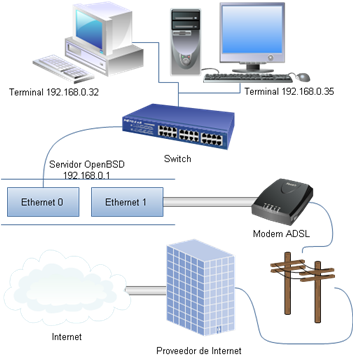
\includegraphics{imagenes/general/conexion_detallada}
	\caption{Esquema de conexi�n detallada de varios equipos de escritorio con el servidor OpenBSD.}
	\label{fig:conexion_detallada_openbsd}
	\end{center}
\end{figure}

En la figura \ref{fig:conexion_detallada_openbsd}, puede verse un esquema detallado de una de nuestras redes locales, conectada a Internet, a trav�s del proveedor de servicios.
%Tambi�n se puede ver en la figura \ref{fig:conexion_detallada_openbsd}, que luego de llegar el cable al poste telef�nico, este sale del troncal local y va a las oficinas de comunicaci�n, que a su vez lo transmiten con el proveedor de servicios (en nuestro caso es Telecom).

\section{Automatizaci�n del sistema}
\label{sec:automatizacion_conexion}

En esta secci�n se detallar�n los pasos necesarios para realizar una conexi�n a Internet automatizada; con todos los servicios que se brindar�n sin necesidad de interacci�n con el terminal del servidor. Es decir, cuando se encienda el equipo se ``levantar�n'' autom�ticamente los servicios correspondientes y la conexi�n a Internet.

Tambi�n se mostrar� la manera de mantener un dominio asociado a la direcci�n IP asignada por el proveedor con el fin de facilitar la conexi�n necesaria entre los servidores de nuestras redes locales.

\subsection{Conexi�n a Internet}

Para que no sea necesario acceder al servidor cada vez que se quiera conectar a Internet, sino que, con solo encender el equipo se efect�e dicha conexi�n de forma autom�tica, se deben crear y/o modificar algunos archivos de configuraci�n.

En primer lugar el archivo ``/etc/rc.local'' contiene los \emph{scripts} que se ejecutan en el arranque del sistema, despu�s de los servicios como Bind, DHCP, etc. En el listado de Configuraci�n \ref{config:conexion_internet_rc.local} se puede ver una secci�n que permite la conexi�n a Internet mediante la ejecuci�n del comando ``ppp -ddial proveedor'' y en el que espera unos segundos antes de ejecutar el comando que comprueba si la conexi�n se ha establecido o no.

\begin{configuracion}
\begin{listing}[style=configuracion]
echo -n 'Estableciendo PPPoE DSL: '; ppp -ddial proveedor
echo -n 'Estableciendo conexion: '
for i in 10 9 8 7 6 5 4 3 2 1 0; do
    sleep 3
    echo -n "$i"
    if /usr/local/sbin/adsl-status > /dev/null; then
        break
    fi
done
echo -n '\nEstado: '; /usr/local/sbin/adsl-status
\end{listing}
\caption{Script para el inicio autom�tico de la conexi�n a Internet.}
\label{config:conexion_internet_rc.local}
\end{configuracion}

Lo que hace el script \ref{config:conexion_internet_rc.local} es llamar al comando ppp para que se conecte con ``proveedor'' definido en /etc/ppp/ppp.conf y esperar unos segundos (sleep) por diez veces, hasta que otro script (adsl-status) devuelva verdadero, es decir que devuelva la direcci�n IP asignada por el proveedor. A este �ltimo script se lo debe crear y darle permisos de ejecuci�n:

\begin{listing}[style=consola, numbers=none]
$ sudo touch /usr/local/sbin/adsl-status
$ sudo chmod +x /usr/local/sbin/adsl-status
$
\end{listing}

Luego se lo edita como aparece en el listado de Configuraci�n \ref{config:adsl-status}.

\begin{configuracion}
\begin{listing}[style=configuracion]
#!/bin/sh

IP=$(/sbin/ifconfig tun0 | awk '/netmask/{print $2}')

if [ -z "$IP" ]; then
   echo "Enlace ADSL no esta conectado."
   exit 1
else
   echo "ADSL conectado, Direccion IP $IP"
   exit 0
fi
\end{listing}
\caption{Script para obtener la direcci�n IP que asigna el proveedor.}
\label{config:adsl-status}
\end{configuracion}

De esta manera, cada vez que arranque el sistema, se iniciar�n los servicios por defecto (como SSH, Inetd, etc.), junto a los servicios que se han indicado manualmente para que se iniciaran como Packet Filter y el script de conexi�n a Internet.

Aunque en realidad OpenBSD ejecuta autom�ticamente todos los comandos que se introduzcan en ``/etc/rc.local'', por eso se debe que tener especial cuidado al editar el archivo, sino pueden ocurrir errores al inicio y si no se monitorea el arranque para ver los mensajes del sistema, ser�a dif�cil conocer el error que se produzca. Por eso es recomendable al principio monitorear todos los mensajes de arranque del sistema.

\subsection{Asociando un nombre de dominio}

En primer lugar es necesario tener un dominio registrado en \href{http://www.nic.ar}, cuyos pasos se pueden resumir como sigue:

\begin{enumerate}
	\item Registrar persona,
	\item Registrar entidad,
	\item Registrar dominio.
\end{enumerate}

El tr�mite a veces es un poco largo, pero lo m�s importante a la hora de registrar el dominio, es ya que se deben agregar como servidores DNS a los que provee el servicio de DNS gratuito para asociar la IP al dominio. De los servicios m�s conocidos se pueden encontrar a:

\begin{itemize}
	\item Zoneedit,
	\item DnsExit,
	\item Entre otros.
\end{itemize}

El que se va a utilizar para esta tesis es Zoneedit, que es gratuito y permite asociar hasta 5 dominios sin costo. Luego del registro, se debe indicar nombre de dominio inicial, y a continuaci�n se obtiene los DNS necesarios para ingresarlos en nic.ar.

\subsection{Actualizaci�n de la direcci�n IP}

Para actualizar el dominio a la direcci�n IP que asigna el proveedor existen varios m�todos que se pueden utilizar con Linux u OpenBSD. Los m�s sencillos son usando la l�nea de comandos, con los programas Lynx o Wget con las siguientes sintaxis:

\begin{listing}[style=consola, numbers=none]
# lynx -source -auth=username:password 'http://dynamic.zoneedit.com/auth/dynamic.html?host=www.mydomain.com'
# wget -O - --http-user=username --http-passwd=password 'http://dynamic.zoneedit.com/auth/dynamic.html?host=www.mydomain.com'
#
\end{listing}

Como OpenBSD no viene con wget de serie y para no instalar ning�n programa adicional, es mejor usar Lynx (que por cierto, no es mucho problema). A ejecutar alg�n comando anterior, se deber�a obtener el mensaje de que ha sido actualizado el dominio a la direcci�n IP que ha asignado el proveedor al equipo servidor.

Como se quiere automatizar todo el proceso, lo mejor es instalar el paquete \emph{ddclient} mediante el comando (suponiendo que se utiliza los repositorios de Argentina):

\begin{listing}[style=consola, numbers=none]
# sudo pkg_add -v http://openbsd.md5.com.ar/pub/OpenBSD/4.3/packages/i386/ddclient-3.7.2.tgz
\end{listing}

Luego de la instalaci�n, se crea el directorio y archivo de configuraci�n en /etc/ddclient. Para terminar la configuraci�n se tiene que modificar, con los datos de la cuenta en Zoneedit, el archivo \texttt{ddclient.conf} que debe contener como m�nimo lo que se muestra en el listado de Configuraci�n \ref{config:zoneedit}.

\begin{configuracion}
\begin{listing}[style=configuracion]
daemon=300                            # check every 300 seconds
syslog=yes                            # log update msgs to syslog
mail=gustavo                          # mail all msgs to root
mail-failure=gustavo                  # mail failed update msgs to root
pid=/var/run/ddclient.pid             # record PID in file.
ssl=yes                               # use ssl-support.Works with ssl-library
use=web                               # via web
##
## ZoneEdit (zoneedit.com)
##
server=www.zoneedit.com,     \
protocol=zoneedit1,          \
login=nomre_cuenta,          \
password=SuP3rS3cr3tP@sS     \
nombrededominio.com.ar
\end{listing}
\caption{Resumen de configuraci�n para ZoneEdit.}
\label{config:zoneedit}
\end{configuracion}

Ahora es necesario ejecutar ddclient y probar su funcionamiento. Los par�metros que utiliza son muy sencillos, pero si ya se ha editado el archivo de configuraci�n, no har�n falta par�metros adicionales, pero por ejemplo para ejecutarlo como ``daemon'', que env�e informaci�n a Syslog y cualquier otra informaci�n a una cuenta de correo local, se deber�a ejecutar ddclient con los siguientes argumentos:

\begin{listing}[style=consola, numbers=none]
# ddclient -daemon=0 -syslog -quiet retry -mail gustavo
\end{listing}

De otra manera, con solo ejecutar ``ddclient'' sin argumentos, se deber�a ver un proceso similar a este:

\begin{verbatim}
8776 C0- I       2:49.43 perl: ddclient - sleeping for 280 seconds (perl)
\end{verbatim}

Como se hab�a indicado en el archivo de configuraci�n, ddclient se ejecuta (en busca de cambios en la direcci�n IP) cada 300 segundos. Adem�s para saber que el dominio se ha actualizado, ddclient env�a un mensaje al usuario designado con la informaci�n siguiente (por ejemplo):

\begin{verbatim}
SUCCESS:  updating nombrededominio.com.ar: IP address set to 190.226.158.2 
(200: Update succeeded.)
regards,
   ddclient@superhijitus.red.lan (version 3.7.1)
\end{verbatim}

Si ocurre alg�n error, tambi�n se notifica por correo. Adem�s OpenBSD env�a informaci�n diaria del estado del sistema, si se han modificado archivos de configuraciones, el promedio de uso del equipo, y otra informaci�n con respecto al uso del disco r�gido y sus particiones. Por esta raz�n es importante tener bien configurado Sendmail al menos para usuarios locales.

En cuanto a \texttt{ddclient}, se lo puede agregar al archivo /etc/rc.local para que inicie autom�ticamente con el sistema, pero antes se debe tener en cuenta de estar conectado a Internet, por eso se lo ejecuta posteriormente al script de conexi�n, agregando la l�nea a continuaci�n:

\begin{verbatim}
echo -n 'Estableciendo dominios... '; 
/usr/local/sbin/ddclient -file /etc/ddclient/ddclient.conf
\end{verbatim}

\subsection{Utilidades de un dominio propio}

El inter�s de tener un dominio asociado a la direcci�n IP que es asignada por el proveedor, puede provenir de que se quiera alojar un servidor Web, por ejemplo, para poder acceder a �l desde otro sitio f�sico. Tambi�n puede resultar importante para establecer una conexi�n por SSH para realizar tareas administrativas.

En el caso de las VPN, para establecer una conexi�n entre dos redes a trav�s de Internet, el hecho de tener un nombre de dominio asociado a nuestra direcci�n IP resulta �til, ya que para establecer la conexi�n debemos conocer dicha direcci�n. Asociar un nombre a una direcci�n IP resulta tambi�n muy econ�mico para las empresas que no puedan afrontar los costos de una soluci�n VPN comercial ni de direcciones IP fijas; pero a su vez es peligroso, debido a que se corre el riesgo de perder la conexi�n, cuando el nombre de dominio no est� apuntando a la direcci�n IP correcta.

\section{Configuraci�n de los clientes}
\label{sec:configuracion_clientes_openbsd}

Hasta ahora solamente se ha hablado de establecer la conexi�n a Internet con el servidor OpenBSD y que permite la conexi�n de los clientes a Internet a trav�s de la puerta de enlace del mismo.

Pero si la configuraci�n en los clientes no se ha realizado adecuadamente es posible que nunca se pueda conectar a Internet desde un terminal. Por esto, hay que configurar a los clientes para que tengan direcci�n IP fija y que pertenezcan a la red del servidor (por ejemplo a la red 192.168.0.0). Adem�s su puerta de enlace debe apuntar a la direcci�n IP de servidor y los DNS pueden ser del servidor local (si es que se brinda dicho servicio) o del proveedor.

Si se tienen varios equipos terminales, con diferentes sistemas operativos, la mejor soluci�n es configurar un servidor \emph{DHCP} en el servidor, para evitar asignar direcciones IP manualmente a cada computadora. En BSD el cliente de DHCP se denomina \emph{dhclient} y se puede configurar para iniciar en el arranque. En Linux y Windows tambi�n se tiene por defecto un cliente DHCP, por lo que en la mayor�a de los casos no se requiere ninguna configuraci�n manual.

\subsection{Servidor DHCP}

Un servidor DHCP permite asignar autom�ticamente direcciones IP de determinado rango a los terminales clientes (equipos de la red local). Esta funcionalidad permite ahorrar mucho tiempo y esfuerzo en lo que ser�a configurar manualmente direcciones IP y Gateway en cada equipo nuevo que se una a la red.

Para que el servicio se inicie durante el arranque del sistema, se tiene que cambiar el par�metro ``NO'' por lo siguiente:

\begin{verbatim}
dhcpd_flags=""
\end{verbatim}

Luego se tiene que editar la configuraci�n del servidor DHCP donde se indica el rango de direcciones IP y los servidores de nombre (DNS) que se les va a transmitir utilizar a los usuarios. El primer archivo es el ``/etc/dhcpd.conf'' que deber�a contener lo siguiente (por ejemplo) lo que se muestra en el listado de Configuraci�n \ref{config:dhcp1}.

\begin{configuracion}
\begin{listing}[style=configuracion]
shared-network LOCAL-NET {
        option  domain-name "red.lan";
        option  domain-name-servers 192.168.0.1;

        subnet 192.168.0.0 netmask 255.255.255.0 {
                option routers 192.168.0.1;

                range 192.168.0.32 192.168.0.127;
        }

}
\end{listing}
\caption{Ejemplo de configuraci�n de un servidor DHCP.}
\label{config:dhcp1}
\end{configuracion}

El otro archivo de configuraci�n es donde se indica la interfaz por la que ``entrar�n'' los cliente a solicitar la informaci�n de la red. Este archivo es ``/etc/dhcpd.interfaces'' y por ejemplo puede contener solamente el dispositivo de red que este conectado al switch:

\begin{verbatim}
rl0
\end{verbatim}

De esta manera se tiene configurado un servidor DHCP para que acepte conexiones a trav�s de la red local (interfaz rl0) y asigne un rango de direcciones IP que van de 192.168.0.32 a 192.168.0.127, lo cual permite a 95 clientes simult�neamente. Los clientes solo deben saber que tienen que buscar un servidor DHCP.

\subsection{Finalizando la configuraci�n}

Ahora que se tiene un sistema robusto, seguro y muy flexible en cuanto a la configuraci�n del mismo, se puede proceder a realizar unos retoques finales en algunos par�metros de configuraci�n.

Para listar los servicios que se est�n ejecutando en el sistema se utiliza el comando ``ps ax'', que puede generar una salida como la siguiente:

\begin{listing}[style=consola, numbers=none]
$ ps ax
  PID TT  STAT       TIME COMMAND
    1 ??  Is      0:00.06 /sbin/init
20075 ??  Is      0:01.72 syslogd: [priv] (syslogd)
11440 ??  I       0:07.20 syslogd -a /var/named/dev/log -a /var/empty/dev/log
23321 ??  Is      0:00.05 pflogd: [priv] (pflogd)
 4388 ??  I       0:19.11 pflogd: [running] -s 116 -i pflog0 -f /var/log/pflog (pflog
 2601 ??  Is      0:00.03 named: [priv] (named)
23128 ??  I       1:15.80 named
23920 ??  Is      0:00.11 /usr/sbin/dhcpd rl0
32432 ??  Is      0:00.23 inetd
 5577 ??  Is      0:00.07 /usr/sbin/sshd
14417 ??  Is      0:29.58 sendmail: accepting connections (sendmail)
20139 ??  Is      0:01.32 cron
10485 ??  Is      0:07.62 sshd: gustavo [priv] (sshd)
32341 ??  I       0:31.25 sshd: gustavo@ttyp0 (sshd)
28682 ??  Is      7:23.01 ppp -ddial arnet
25835 ??  I       2:19.97 /usr/sbin/pppoe -i ne1
 9284 ??  Is      0:00.01 /usr/local/bin/svnserve -d --listen-host 192.168.0.1 -r /va
24124 ??  Is      0:00.12 /usr/local/bin/svnserve -d --listen-host 190.137.64.32 -r /
28303 p0  Is      0:00.96 -ksh (ksh)
14206 p0  R+      0:00.00 ps -ax
 8776 C0- I       2:55.17 perl: ddclient - sleeping for 50 seconds (perl)
22579 C0  Is+     0:00.06 /usr/libexec/getty std.9600 ttyC0
$
\end{listing}

En el listado anterior se pueden ver los servicios que se han configurado para iniciar junto a los argumentos con que se ejecutan. Tambi�n se pueden ver otros servicios como los dos servidores de Subversion (Secci�n \ref{appendix:doc_control_versiones} de la p�gina \pageref{appendix:doc_control_versiones}) e Inetd.

El servicio Inetd es un conjunto de servicios que se inician de acuerdo a la demanda o solicitud de un servicio determinado. En muchos casos es conveniente desactivar estos servicios para no abrir puerto innecesarios, ya que los servicios b�sicos que ofrece (como ftp, finger, ident, pop3, daytime, entre otros) trabajan en texto claro, en el que por ejemplo el servicio POP3 que utiliza autenticaci�n para funcionar, env�a los datos de usuarios sin encriptar, de manera que con un simple sniffer de paquetes se pueden obtener nombres de usuarios y contrase�as en texto claro. 

Si por otro motivo se requiere utilizar alguno de estos servicios, los datos de los mismos se encuentran en /etc/inetd.conf y para habilitarlos basta con quitar el comentario de una l�nea o comentarla para deshabilitar el servicio. 

Por otro lado, las conexiones de terminales se pueden limitar a solamente una terminal virtual, de manera que se libera memoria innecesaria (para administrar el sistema, pocas veces se puede llegar a usar m�s de un terminal). El archivo de terminales se encuentre en /etc/ttys, y solo es necesario que cambiar el valor ``on'' por el valor ``off'':

\begin{verbatim}
console "/usr/libexec/getty std.9600"   vt220   off secure
ttyC0   "/usr/libexec/getty std.9600"   vt220   on  secure
ttyC1   "/usr/libexec/getty std.9600"   vt220   off secure
\end{verbatim}

Para mejorar la seguridad del sistema, se puede quitar la contrase�a del usuario \emph{root} para evitar cualquier intrusi�n o intento de hacking a esta cuenta. Para esto, se debe suponer que un usuario normal pueda tener permisos de ejecuci�n del comando ``sudo'' para poder realizar las operaciones de administraci�n del sistema. Para agregar un usuario al grupo \emph{wheel} (para poder ejecutar ``sudo''), es necesario el comando ``gpasswd -a <usuario> wheel''. Adem�s es necesario asegurar de que al ejecutar \texttt{visudo} para editar el archivo de configuraci�n de sudo, �ste contenga la l�nea:

\begin{verbatim}
%wheel  ALL=(ALL) SETENV: ALL
\end{verbatim}

Y luego quitar la contrase�a de root, eliminando la cadena de texto \emph{extra�o} del archivo \texttt{master.passwd} de manera que quede como sigue:

\begin{verbatim}
root::0:0:daemon:0:0:Root &:/root:/bin/ksh
\end{verbatim}

De esta manera, nadie va a poder ingresar como \emph{root}. Pero a pesar de que esto puede suponer una mejora para la seguridad del sistema, por otro lado se debe tener en cuenta que el usuario del sistema con permisos en el grupo wheel, no puede tener una contrase�a d�bil, ya que puede ser descifrada y utilizada como si del usuario \emph{root} se tratara (ya que en la configuraci�n de \texttt{visudo} se ha especificado que el usuario que pertenezca a \emph{wheel} pueda ejecutar cualquier comando como administrador). Otra manera de asegurar el sistema ser�a especificar que los usuarios \emph{wheel} solo tengan permiso de administrar determinados archivos y entornos, que tambi�n se consigue editando la configuraci�n con \texttt{visudo}.

\section{Recursos utilizados}
\label{sec:conexion_internet_recursos}

En esta secci�n se describen los aspectos superficiales y econ�micos de los componentes utilizados para la conexi�n a Internet de la red local. Para m�s detalles en la descripci�n de equipos de toda la VPN, ver el Ap�ndice \ref{appendix:equipos_de_prueba}.

\subsection{Servidor}

El servidor debe ser una m�quina medianamente potente y en buen funcionamiento. Debe tener su gabinete en buenas condiciones y con los ventiladores correspondientes y en buen estado. Es importante mantener estas caracter�sticas, ya que el equipo debe estar encendido siempre, por lo que la refrigeraci�n es punto clave para mantener un buen servicio y funcionamiento del servidor, adem�s de alargar la usabilidad del mismo. Si no se dispone de un PC para el servidor, hoy en d�a existe la posibilidad de comprar equipos de marca muy econ�micos, con respecto a la utilidad que se le dar�.

\subsection{Modem ADSL y Switch}

El modem ADSL y Switch son componentes que hay que elegirlos en cajas cerradas, ya que no se pueden ``fabricar'', pero se deben tener muy en cuenta de la calidad de lo que se adquiere.

En cuanto al modem ADSL, debe contar con una interfaz Ethernet para conectar la placa de red del servidor, que en general son m�s costoso que los modem con solo puerto USB. El precio de estos dispositivos no superan los 200 pesos, cumpliendo la �nica funci�n de ``bridge'' entre la interfaz Ethernet y la l�nea telef�nica.

El switch tambi�n es un elemento muy com�n usado en redes de cualquier tama�o y se pueden conseguir a un precio muy econ�mico.

\subsection{Cableado}

El cableado es un componente importante que afecta en el rendimiento de la red. Muchas veces la deficiente comunicaci�n entre hosts se debe a una mala instalaci�n de los cables de red. Para ver que la velocidad de conexi�n es adecuada, basta con una simple transmisi�n de archivos entre las terminales. Si se trata de una red a 100 Mbps, la velocidad te�rica a alcanzar deber�a ser de 12,5MB/s, aunque si se alcanza un 75 o 90 por ciento est� muy bien tambi�n.

Hoy en d�a, como todos los switch soportan las normas de cableado 568-B (normal) y 568-A (cruzado), lo m�s conveniente es armar directamente cables cruzados, por si alguna vez deja de funcionar el switch o se necesita hacer pruebas conectando solo dos hosts.

La categor�a del cable a utilizar tambi�n es importante, y actualmente es f�cil conseguir Cat-5e a precios razonables (menos de 2 pesos el metro).

\section{Conclusi�n}
\label{sec:conexion_conclusion}

Hoy en d�a la conexi�n a Internet es un requisito casi imprescindible para el funcionamiento y crecimiento de una empresa. Por esta raz�n es que se ha dedicado todo un cap�tulo a la configuraci�n de la misma.

Si bien se podr�an haber planteado alternativas para la conexi�n a Internet, se considera que la mejor soluci�n es dedicar un equipo completo que realizara tal funci�n, ya que permite la flexibilidad de configuraci�n del sistema, el considerable aumento de la seguridad al tener firewall robustos y la posibilidad de incluir servicios adicionales como servicios de direcciones IP din�micas, asignaci�n autom�tica de direcci�n IP local, administraci�n remota, entre otros.

Adem�s los bajos requisitos de los equipos hacen muy econ�mica su adquisici�n, ya que no requiere potencia en gr�ficos, ni grandes cantidades de espacio de almacenamiento. Pero lo m�s importante y a veces costoso se refiere al mantenimiento de los equipos, ya que si se mantiene la conexi�n las 24 horas al d�a, el equipo levanta temperatura, y puede da�ar los componentes. Por eso la importancia de tener una buena refrigeraci�n.

En cuanto a los sistemas operativos que pueden instalarse en los equipos, se cuenta con una gran variedad (entre Linux, BSD, Solaris, etc.), pero se ha elegido OpenBSD en particular por su elevada seguridad y bajos requerimientos para un funcionamiento fluido. Tambi�n tiene una gran cantidad de informaci�n en Internet para resolver los distintos problemas que se vayan presentando.


%% VPN con PPTP
%%%%%%%%%%%%%%%%%%%%%%%%%%%%%%%%%%%%%%%%%%%%%%%%%%%%%%%%
%   |-------------------------|                        %
%   |REDES PRIVADAS VIRTUALES |                        %
%   |                         |                        %
%   | Proyecto de graduaci�n  |                        %
%   |_________________________|                        %
%                                                      %
%   Autores                                            %
%   -------                                            %
%                                                      %
% * Formoso Requena, Nicol�s Federico (CX02-0239-8)    %
%     nicolasformoso@gmail.com                         %
% * Cortez, Gustavo Maximiliano (CX01-0801-9)          %
%     cmgustavo83@gmail.com                            %
%                                                      %
%   Tutores                                            %
%   -------                                            %
%                                                      %
% * Ing. Gustavo Vanetta - vanettag@gmail.com          %
% * Lic. Miguel Bazzano - miguelbazzano@gmail.com      %
%                                                      %
%%%%%%%%%%%%%%%%%%%%%%%%%%%%%%%%%%%%%%%%%%%%%%%%%%%%%%%%

% ************* VPN con PPTP *************** %

\chapter{VPN usando PPTP}
\label{chap:proto_pptp}

PPTP es un protocolo dise�ado para establecer comunicaciones seguras entre dos terminales, que luego se terminaron usando para establecer una VPN de tipo host a host (o en algunos casos, host a red). En este cap�tulo se describir� brevemente el protocolo junto a sus ventajas y desventajas de uso.

Tambi�n se explicar� la configuraci�n de PPTP a trav�s de Internet (utilizando tanto Windows como Linux y OpenBSD), teniendo en cuenta que el usuario se encuentra en una red local, por lo que se mostrar�n los detalles de configuraci�n del firewall y los par�metros necesarios para establecer una VPN con PPTP.

\section{Introducci�n a PPTP}
\label{sec:pptp_introduccion}

El protocolo \gls{PPTP} ha sido desarrollado por Microsoft, U.S. Robotics, Ascend Communications, 3Com/Primary Access, ECI Telematics conocidas colectivamente como PPTP Forum, para implementar redes privadas virtuales y asegurar conexiones punto a punto.

PPTP se utiliza de manera m�s espec�fica para crear sesiones VPN para usuarios m�viles en configuraciones host a red o host a host. La integraci�n que tiene PPTP con Windows es nativa, pero con otros sistemas operativos, se utilizan portes o adaptaciones que siguen las especificaciones del protocolo.

El �nico motivo por el que se requiere de una implementaci�n del protocolo para sistemas Linux o BSD, es para dar soporte a la gran cantidad usuarios m�viles que utilizan Windows, ya que para establecer una conexi�n host a host con el mismo sistema operativo, el proceso de configuraci�n no resulta para nada complicado.

\subsection{Funcionamiento de PPTP}

PPTP utiliza para establecer conexiones VPN seguras. Primero, realiza el encapsulado de los paquetes de datos dentro de paquetes PPP. Luego se encapsulan estos paquetes usando el protocolo \gls{GRE} y se los env�a al otro extremo del enlace.

Adem�s de los paquetes GRE, que comprimen los datos PPTP reales, se utiliza un segundo canal de control para la conexi�n. Esta es una conexi�n \gls{TCP} sencilla desde el cliente al puerto 1723 del servidor. Se la utiliza para enviar informaci�n de se�alizaci�n y para comprobar el estado de la conexi�n PPTP.

Por otro lado, PPTP no especifica qu� algoritmos de cifrado o autenticaci�n utilizar, sino que esta tarea queda para la sesi�n PPP subyacente.

\subsection{Autenticaci�n y cifrado}

Para permitir autenticaci�n y cifrado en la sesi�n PPTP, se han tenido que a�adir unos cuantos algoritmos a PPP. Para la autenticaci�n, se ha a�adido una variante de \gls{CHAP}, llamada \gls{MS-CHAP}. Este se basa en dos m�todos de Microsoft utilizados para la autenticaci�n y compartimiento de archivos: el algoritmo de dispersi�n LAN Manager (basado en el cifrado DES) y el algoritmo de dispersi�n Windows NT (basado en la funci�n de dispersi�n MD4).

La segunda extensi�n de PPP es el protocolo \gls{MPPE} que maneja el cifrado real de los paquetes. Utiliza el cifrado de flujo RC4 para cifrar los datos con una clave de 40 a 128 bits. La clave de cifrado utilizada para el cifrado deriva parcialmente de la contrase�a del usuario mediante el algoritmo LAN Manager o el algoritmo NT. Las claves de sesi�n utilizadas para el cifrado se cambian peri�dicamente, normalmente despu�s de cada 256 paquetes.

\section{PPTP con Windows}
\label{sec:pptp_servidor_windows}

En esta secci�n se mostrar� c�mo configurar un servidor VPN en Windows Vista, de la manera m�s simple posible, que permite varias conexiones entrantes mediante autenticaci�n por nombre de usuario y contrase�a.

Como no se trata de un servidor \emph{dedicado}, sino m�s bien de una estaci�n de trabajo que se configura para aceptar conexiones de otros clientes, la puesta a punto de la misma puede estar al alcance de cualquier usuario de oficina. Esto podr�a considerarse una falla de seguridad, ya que al permitir conexiones entrantes ajenas a la red interna sin considerar una pol�tica de seguridad adecuada, puede suceder que la conexi�n permitida no sea quien dice ser (es decir, sea un hacker con malas intenciones).

Para solventar este problema, se realizar�n retoques en la configuraci�n del firewall de la red, para permitir conexiones entrantes solamente a los equipos supervisados y autorizados para dicha funci�n.

\subsection{Modo de conexi�n}

Para comunicar dos equipos utilizando el protocolo PPTP se realiza una conexi�n de tipo host a host, entre terminales con el sistema operativo Windows.

Una VPN host a host (o punto a punto) involucra �nicamente a dos equipos, donde uno act�a como servidor y el otro como cliente. Estos pueden estar ubicados en puntos muy distantes o en subredes distintas. Solamente si se puede establecer una ruta de comunicaci�n entre ambos terminales, se podr� realizar la conexi�n VPN.

Este tipo de conexiones, en apariencia tan limitadas, encuentran su fin pr�ctico cuando dos servidores de una empresa necesitan sincronizar datos confidenciales, y deben hacerlo a trav�s de redes de acceso p�blico donde se corre el riesgo de que los datos sean interceptados por destinos no deseados. De esta manera, los datos viajan seguros a trav�s de un medio hostil. Un esquema simplificado de este tipo de conexi�n se puede ver en la Figura \ref{fig:esquema_hostahost}.

\begin{figure}[htbp]
	\begin{center}
	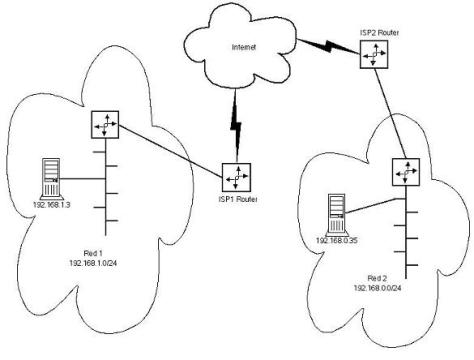
\includegraphics{imagenes/host-host/esquema_h2h}
	\caption{Esquema de conexi�n de las redes utilizadas.}
	\label{fig:esquema_hostahost}
	\end{center}
\end{figure}

\subsection{Directivas del Firewall}

Para aceptar conexiones entrantes del cliente se debe abrir el puerto 1723 (PPTP) tanto para paquetes TCP como para UDP, y adem�s de permitir paquetes que utilicen el protocolo GRE, tanto a la entrada como a la salida de datos.

\begin{configuracion}
\begin{listing}[style=configuracion]
# Redireccionamiento de paquetes al servidor VPN 
rdr pass on $ext_if proto tcp from any to any port pptp -> $server_vpn
rdr pass on $ext_if proto gre from any to any -> $server_vpn
 
# Reglas de filtrado para la entrada y salida de conexiones VPN. 
pass in quick on $ext_if proto tcp from any to any port pptp \ 
	flags S/FSRA keep state

# Paquetes GRE para conexion VPN saliente
pass on $ext_if proto gre from any to any
\end{listing}
\caption{Aceptar conexiones PPTP y GRE.}
\label{config:config_host_to_host}
\end{configuracion}

Estas directivas requieren peque�as modificaciones en el Packet Filter, tal como se muestra en el C�digo \ref{config:config_host_to_host}. Luego de agregar estas l�neas, se debe volver a recargar PF con \emph{pfctl -f /etc/pf.conf}.

\subsection{Aceptar conexiones con Windows Vista}

La configuraci�n de un servidor VPN en Windows Vista resulta m�s sencilla cuando se trata de una comunicaci�n simple de tipo host a host. En primer lugar lo que se crea es una conexi�n entrante, que permita el ingreso de conexiones desde el exterior a la red \emph{virtual}.

Para que esta comunicaci�n pueda establecerse, hay que configurar el firewall del equipo, ya que hoy en d�a todas las computadoras personales disponen de alg�n antivirus con firewall incorporado con el fin de evitar el ingreso de intrusos que pongan en peligro los datos personales, que desde el punto de vista del usuario son m�s importantes que los fallos del sistema (que puede solucionarse en la mayor�a de los casos con una simple reinstalaci�n), pero como administrador de una red local, en la que no solo se considera importante la p�rdida de datos de un usuario, sino tambi�n de la seguridad del sistema y de toda la red, al establecerse una comunicaci�n VPN se la realiza con el firewall activado y configurado para bloquear todas las conexiones entrantes y evitar que clientes poco precavidos pongan en riesgo la seguridad de toda la red.

La configuraci�n del firewall consta en habilitar el compartir archivos de Windows y el puerto PPTP que se utiliza en las conexiones punto a punto entre equipos con sistemas de Microsoft. Luego, entra en acci�n el equipo servidor de VPN, el cual realiza la negociaci�n de la conexi�n estableciendo el tipo de encriptaci�n, de protocolos que se van a utilizar y del m�todo que se env�a la contrase�a. Una vez establecidos estos par�metros, el sistema le asigna una direcci�n IP (puede ser cualquier direcci�n IP privada v�lida, siempre que no interfiera con los rangos ya seleccionados) al cliente, estableciendo la conexi�n propiamente dicha.

\begin{figure}[htb]
	\begin{center}
	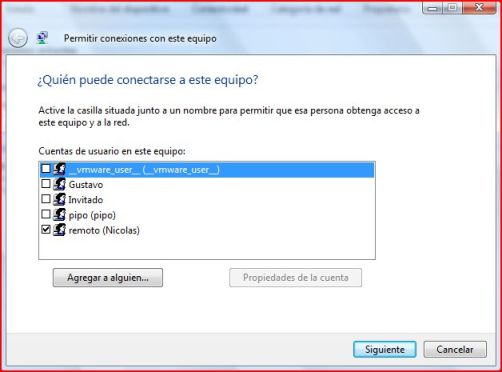
\includegraphics{imagenes/host-host/conf_server2}
	\caption{Usuarios permitidos para conectarse a la VPN.}
	\label{fig:conexiones_usuarios}
	\end{center}
\end{figure}

En Windows Vista el asistente para crear una conexi�n entrante resulta sencillo e intuitivo de usar, ya que las opciones por defecto son en general la mejor elecci�n. Al abrir la ventana de administraci�n de interfaces de red, se visualizan las conexiones establecidas, en la que se muestran detalles como la direcci�n asignada, m�scara de red, servidor DNS primario y secundario asignados, direcciones MAC, entre otros.

La elecci�n de un usuario para que se conecte con el equipo servidor puede ser muy cr�tica a la hora de mantener la seguridad del sistema (y por qu� no, de toda la red), ya que dar a alguien privilegios de administrador y contrase�a f�cil de romper, puede significar un gran problema de seguridad (Figura \ref{fig:conexiones_usuarios}). En este caso, se crea un usuario espec�fico para la conexi�n VPN, al cual se le asignan los permisos necesarios para las acciones m�nimas en la red (como copiar archivos del servidor). 

\begin{figure}[htb]
	\begin{center}
	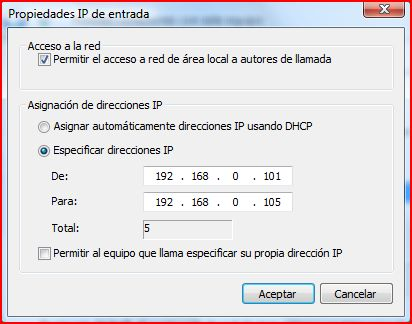
\includegraphics{imagenes/host-host/conf_server5}
	\caption{Direcciones IP habilitadas para asignar a los usuarios.}
	\label{fig:conexiones_ip}
	\end{center}
\end{figure}

El asistente de configuraci�n de conexiones entrantes tambi�n pregunta por el software de red que se le habilitar� a los usuarios que se conecten a la VPN, seleccionando por defecto las opciones de \gls{TCP}/\gls{IPv4}, de compartir archivos e impresoras y de calidad de servicio. Pero para que funcionen estos servicios se debe configurar el firewall local para aceptar este tipo de conexiones.

Como �ltima opci�n del asistente, se pueden configurar las direcciones IP que se les dar�an a los usuarios, permitiendo asignar direcciones que pertenezcan a otra red y as� diferenciar la red local de la red VPN. En la Figura \ref{fig:conexiones_ip} se puede ver que el total de conexiones es de 5 usuarios, pero uno de ellos representa el servidor de VPN, que establece un puente virtual entre el sistema local y la nueva interfaz de red (que se crea autom�ticamente).

Si se escribiera un grupo de direcciones IP que pertenecen a una subred diferente (por ejemplo: 192.168.1.0), el asistente de configuraci�n de conexi�n entrante, configurar� autom�ticamente la tabla de ruteo para exista una comunicaci�n entre la red actual y la creada para la VPN. 

Por otro lado es importante se�alar, que a la primera conexi�n entrante, el sistema crea una nueva entrada en la tabla de ruteo que dirige el tr�fico de la VPN hacia la puerta de enlace (servidor de Internet) para todos los paquetes que no pertenezcan a la red local o a la red creada para la VPN. Es decir que adem�s de crear una conexi�n segura entre dos enlaces, tambi�n se puede acceder a Internet sin temer que los mismos miembros de la red registren los paquetes y descubran informaci�n personal del usuario.

\subsection{Cliente PPTP con Windows}
\label{subsec:pptp_configuracion_cliente}

El proceso de configuraci�n del cliente es sencillo y contiene pocos elementos para configurar, ya que solo realiza la conexi�n al servidor y es �ste quien negocia los par�metros establecidos necesarios. En definitiva, la mayor dificultad en cuanto a configuraci�n se encuentra en el servidor.

Para conectar al servidor de VPN, se debe crear en el cliente una nueva conexi�n. Como Microsoft dise�a la mayor�a de sus sistemas operativos para que sus usuarios finales no necesiten conocimientos profundos sobre los mismos, las opciones que se muestran a medida que avanza el asistente de configuraci�n, no contiene muchas especificaciones, como se puede ver en la Figura \ref{fig:config_cliente_2}.

\begin{figure}[htb]
	\begin{center}
	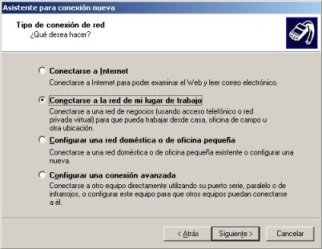
\includegraphics{imagenes/host-host/cliente/ss02}
	\caption{Configuraci�n Cliente, tipo de conexi�n.}
	\label{fig:config_cliente_2}
	\end{center}
\end{figure}

Posteriormente, se debe especificar si el establecimiento de la conexi�n estar� precedido por el de otra, es decir, si para establecer la ruta entre el cliente y el servidor de la VPN, es necesario tener una conexi�n a Internet ya establecida, o a otra red.

En general la conexi�n a Internet ya est� establecida por el servidor de la red local, por lo que en el men� correspondiente se selecciona la opci�n de no utilizar la conexi�n inicial.

Luego se debe especificar el nombre de dominio o la direcci�n IP del servidor VPN. Esto implica que el cliente siempre que quiera conectarse a la VPN deber� conocer la IP del servidor. Por lo que, dicha direcci�n, no debe ser variable, o en su defecto debe existir un nombre de dominio que pueda \emph{seguir} los cambios de la misma. En la secci�n \ref{sec:automatizacion_conexion} se explica c�mo obtener un nombre de dominio permanente, a�n teniendo una direcci�n IP variable.

Terminado el asistente, se puede ver que dentro de ``Conexiones de red'' que se ha creado una nueva conexi�n, que es la que se utiliza para conectar al servidor de la red privada virtual.

\subsection{Resultado}

Establecida la conexi�n VPN, ambos hosts tendr�n la impresi�n de que est�n en una misma subred privada (distinta a la que cada uno de ellos est� conectado realmente); adem�s, los datos transmitidos entre ellos a trav�s de la VPN, ser�n \emph{invisibles} a los dem�s usuarios.

El protocolo de autenticaci�n de claves utilizado es \gls{MS-CHAP} v2; y el algoritmo de cifrado para los mensajes es \gls{MPPE}, de 128 bits.

El esquema resultante de la VPN se muestra en la Figura \ref{fig:pptp_esquema_vpn}.

\begin{figure}[htb]
	\begin{center}
	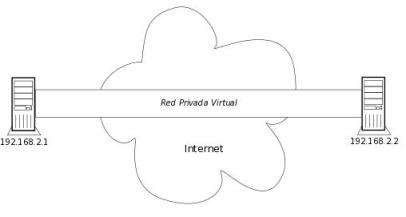
\includegraphics{imagenes/host-host/esquema_vpn}
	\caption{Esquema b�sico de un enlace host a host.}
	\label{fig:pptp_esquema_vpn}
	\end{center}
\end{figure}

\section{PPTP con software libre}
\label{sec:pptp_linux_openbsd}

Con la popularidad de Windows y su protocolo PPTP para establecer enlaces punto a punto seguros, era necesario integrar otros sistemas operativos para permitir este tipo de conexiones, ya que la mayor�a de los clientes de escritorios contaban con Windows como sistema principal.

De esta manera, se ha iniciado el desarrollo de un clon del protocolo de c�digo fuente abierto en conjunto con Microsoft para permitir la integraci�n de equipos Windows con cualquier otro sistema operativo mediante un enlace seguro y compatible con el original PPTP. Este desarrollo se ha denominado PoPToP \footnote{Juego de palabras que, en definitiva, significa PPTP. \href{http://www.poptop.org/}{http://www.poptop.org/}.}.

\subsection{Caracter�sticas de PoPToP}

PoPToP se ha portado a la mayor�a de los sistemas operativos, incluyendo Linux y OpenBSD. Gracias a esto, se pueden integrar sistemas heterog�neos (incluyendo equipos con Windows) mediante un enlace com�n y asegurado por PPTP. Entre las caracter�sticas t�cnicas que tiene PoPToP se pueden listar las siguientes:

\begin{itemize}
	\item Autenticaci�n y encriptaci�n compatible con Microsoft (MSCHAPv2, MPPE 40 - 128 bit RC4 encryption).
	\item Soporte para m�ltiples conexiones.
	\item Mediante el uso de plugin se pueden integrar entronos de redes (LDAP, SAMBA).
	\item Es compatible con el cliente PPTP de Linux.
	\item Es totalmente gratuito bajo licencia GNU (General Public Licence).
\end{itemize}

\subsection{Instalaci�n de PoPToP}

En Linux (Ubuntu Server 8.04) se han realizado las pruebas de conexi�n e interacci�n con sistemas Windows XP y Vista. La instalaci�n de PoPToP no requiere gran intervenci�n por el administrador; se realiza mediante el comando:

\begin{listing}[style=consola, numbers=none]
gustavo@wasa:~$ sudo apt-get install pptpd
...
gustavo@wasa:~$
\end{listing}

De esta manera, se instala el \texttt{daemon} PPTP y se inicia autom�ticamente.

Para establecer una conexi�n fiable, se necesitan modficiar algunos par�metros de configuraci�n, como el rango de direcciones IP que puede aceptar (que limita tambi�n la cantidad de clientes que pueden acceder simult�neamente), los certificados (si es que se utilizan), entre otros.

\subsection{Configuraci�n de PPTP}

Los archivos necesarios para configurar PoPToP correctamente son los siguientes:

\begin{enumerate}
	\item \texttt{/etc/pptpd.conf}
	\item \texttt{/etc/ppp/pptpd-options.conf}
	\item \texttt{/etc/ppp/chap-secrets}
\end{enumerate}

El primer archivo es el utilizado por PoPToP para lanzar el \texttt{daemon} PPTPD, adem�s de las direcciones IP del servidor y las que se asignan a los clientes. En la Configuraci�n \ref{config:pptpd.conf} se puede ver un ejemplo b�sico de funcionamiento.

\begin{configuracion}
\begin{listing}[style=configuracion]
option /etc/ppp/pptpd-options
debug
logwtmp
localip 192.168.2.1
remoteip 192.168.2.2-9
\end{listing}
\caption{Ejemplo de configuraci�n b�sica de PoPToP.}
\label{config:pptpd.conf}
\end{configuracion}

En la primera l�nea se debe indicar el archivo secundario de configuraci�n del daemon PPTPD, que en este caso se encuentra en \texttt{/etc/ppp/pptpd-options}. La segunda l�nea indica que se muestren todos los mensajes en el archivo de registro. La tercera indica que se registren todas las conexiones y desconexiones de los clientes para PPP, ya que por defecto se encuentra habilitada para las otras interfaces (como pts/0 o tty1) y es bastante �til para saber en qu� horarios se conectaron, por cuanto tiempo y cuando se desconectaron los clientes.

Finalmente las �ltimas dos l�neas indican la direcci�n IP del servidor y el rango de direcciones que se les asignan a los clientes respectivamente. Si se supera este rango, no se aceptan m�s conexiones, por lo que en este caso solo se permiten ocho clientes simult�neamente.

\begin{configuracion}
\begin{listing}[style=configuracion]
name pptpd
domain red.lan
refuse-pap
refuse-chap
refuse-mschap
require-mschap-v2
require-mppe-128
ms-dns 192.168.0.1
proxyarp
lock
nobsdcomp
\end{listing}
\caption{Ejemplo de opciones en pptp-options.}
\label{config:pptpd-options}
\end{configuracion}

En el archivo de Configuraci�n \ref{config:pptpd-options} se indican el m�todo de encriptaci�n utilizado, los servidores DNS, el gateway, entre otras opciones. Tambi�n se puede observar que se rechazan conexiones utilizando el m�todo de autenticaci�n antiguo de Microsoft, el \gls{MS-CHAP} versi�n 1 (pero se acepta la versi�n 2), ya que presenta problemas de seguridad debido a que env�a la contrase�a del cliente utilizando el algoritmo LAN Manager que es muy d�bil y luego un \emph{hash} Windows NT que depend�a de la primera. Por lo tanto se podr�a quebrar el algoritmo f�cilmente con la herramienta L0phtcrack\footnote{\href{http://es.wikipedia.org/wiki/L0phtCrack}{http://es.wikipedia.org/wiki/L0phtCrack}}.

El �ltimo archivo es un simple archivo de texto que deber�a tener permisos limitados solo para el propietario (0600), ya que contiene el nombre de usuario y contrase�a de los clientes. Adem�s se incluyen las direcciones IP de los hosts desde los que pueden efectuar la conexi�n, que pueden ser sustituidas por un asterisco para indicar que el usuario puede conectarse desde cualquier equipo.

\subsection{Estableciendo conexi�n}

Para establecer la conexi�n con el servidor PPTP, se utiliza la misma configuraci�n descripta anteriormente en la Secci�n \ref{subsec:pptp_configuracion_cliente}.

Cuando el sistema detecta una conexi�n entrante, realiza el proceso de intercambio de informaci�n, entre los que se encuentra el env�o de las claves del usuario, y finalmente se acepta o rechaza la conexi�n. En caso afirmativo, se muestra la siguiente salida en el registro del sistema:

\begin{listing}[style=consola, numbers=none]
Oct 17 09:23:11 wasa pptpd[5520]: CTRL: Client 190.137.67.68 control connection started
Oct 17 09:23:11 wasa pptpd[5520]: CTRL: Starting call (launching pppd, opening GRE)
Oct 17 09:23:11 wasa pppd[5521]: Plugin /usr/lib/pptpd/pptpd-logwtmp.so loaded.
Oct 17 09:23:11 wasa pppd[5521]: pppd 2.4.4 started by root, uid 0
Oct 17 09:23:11 wasa pppd[5521]: Using interface ppp1
Oct 17 09:23:11 wasa pppd[5521]: Connect: ppp1 <--> /dev/pts/3
Oct 17 09:23:11 wasa pptpd[5520]: GRE: Bad checksum from pppd.
Oct 17 09:23:11 wasa pptpd[5520]: CTRL: Ignored a SET LINK INFO packet with real ACCMs!
Oct 17 09:23:11 wasa pppd[5521]: MPPE 128-bit stateless compression enabled
Oct 17 09:23:13 wasa pppd[5521]: Cannot determine ethernet address for proxy ARP
Oct 17 09:23:13 wasa pppd[5521]: local  IP address 192.168.2.1
Oct 17 09:23:13 wasa pppd[5521]: remote IP address 192.168.2.3
\end{listing}

En este caso se establecen las direcciones IP local (del servidor) y la asignada a la nueva conexi�n. Tambi�n se puede ver que se utiliza una encriptaci�n \gls{MPPE} de 128 bit con compresi�n habilitada.

Los dispositivos que crea cada conexi�n remota PPTP, se denominan por defecto ppp\textbf{X}, donde \textbf{X} es un n�mero que se incrementa por cada conexi�n, comenzando en cero. Por ejemplo la siguiente salida se obtiene del comando \emph{ifconfig}:

\begin{listing}[style=consola, numbers=none]
ppp0      Link encap:Point-to-Point Protocol
          inet addr:192.168.2.1  P-t-P:192.168.2.2  Mask:255.255.255.255
          UP POINTOPOINT RUNNING NOARP MULTICAST  MTU:1396  Metric:1
          RX packets:64 errors:0 dropped:0 overruns:0 frame:0
          TX packets:17 errors:0 dropped:0 overruns:0 carrier:0
          collisions:0 txqueuelen:3
          RX bytes:5610 (5.4 KB)  TX bytes:628 (628.0 B)
          
ppp1      Link encap:Point-to-Point Protocol
          inet addr:192.168.2.1  P-t-P:192.168.2.3  Mask:255.255.255.255
          UP POINTOPOINT RUNNING NOARP MULTICAST  MTU:1396  Metric:1
          RX packets:36 errors:0 dropped:0 overruns:0 frame:0
          TX packets:11 errors:0 dropped:0 overruns:0 carrier:0
          collisions:0 txqueuelen:3
          RX bytes:3667 (3.5 KB)  TX bytes:288 (288.0 B)
\end{listing}

En la salida anterior se puede observar que se han establecido dos conexiones remotas y que se encuentran activas en ese instante. El primer campo de ``inet addr'' corresponde a la direcci�n IP del servidor, mientras que ``P-t-P'' refiere a la direcci�n IP asignada a la conexi�n entrante. Luego se utiliza esta direcci�n IP para establecer las tablas de ruteo:

\begin{listing}[style=consola, numbers=none]
gustavo@wasa:/etc/ppp$ route
Kernel IP routing table
Destination     Gateway         Genmask         Flags Metric Ref    Use Iface
192.168.2.2     *               255.255.255.255 UH    0      0        0 ppp0
192.168.0.0     *               255.255.255.0   U     0      0        0 eth1
default         192.168.0.1     0.0.0.0         UG    100    0        0 eth1
gustavo@wasa:/etc/ppp$
\end{listing}

De lo anterior se puede observar que hay solamente una conexi�n activa (en ppp0) donde se ha establecido la direcci�n IP \texttt{192.168.2.2} al equipo remoto. Pero se ha especificado que no cambie el ruteo ``default gateway'', por lo que se mantiene el servidor anterior ( es decir, la IP \texttt{192.168.0.1} como pasarela predeterminada).

\section{Rendimiento de la conexi�n}
\label{sec:host_to_host_rendimiento_conexion}

Mientras se realizaban las pruebas de conexi�n, se utilizaron sistemas de monitoreo que permiten visualizar gr�ficamente el rendimiento antes y durante la conexi�n VPN establecida. En el servidor, el software se llama \textbf{Monitor de confiabilidad y rendimiento} y viene integrado al sistema operativo.

En la Figura \ref{fig:monitor_vpn} se puede observar el rendimiento de la CPU y consumo de memoria al momento de establecerse la conexi�n entrante del primer usuario al servidor VPN.

\begin{figure}[htb]
	\begin{center}
	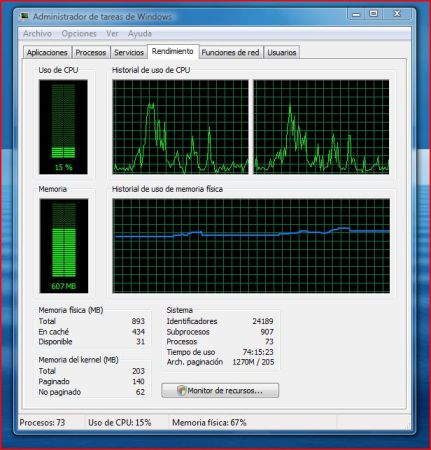
\includegraphics{imagenes/host-host/monitor_sistema_convpn2}
	\caption{Rendimiento del sistema (con el servicio de VPN).}
	\label{fig:monitor_vpn}
	\end{center}
\end{figure}

Para evaluar la comunicaci�n se realizaron varios experimentos, aunque para poder comprobar el rendimiento y comportamiento de la VPN en un entorno de conexi�n real, se necesitan muchas conexiones simult�neas de las que no se dispone, por lo que se realizar�n las evaluaciones con una sola conexi�n activa.

La distancia entre los hosts no supera los 5 saltos (obtenidos mediante el comando \texttt{tracert}). Adem�s el horario en el que se realizan dichas pruebas tiene gran influencia en el rendimiento, por lo que se ha optado por una franja horaria de testeo entre las 9 y 10 de la ma�ana.

\subsection{Escritorio virtual}

Una de las aplicaciones utilizadas para la conexi�n a un escritorio remoto y tener control total del equipo es \textbf{UltraVNC}.

El sistema de escritorio compartido \gls{VNC} fue desarrollado inicialmente por AT\&T para la gesti�n de escritorio remotos. Por su parte microsoft ha desarrollado su propio sistema de administraci�n de escritorio remoto, pero para estas pruebas, se ha utilizado UltraVNC, que es software libre y sirve para el mismo prop�sito. VNC utiliza el protocolo RFB (Remote Framebuffer) para traer la interfaz gr�fica del servidor al cliente, de manera que se visualice en pantalla lo que esta viendo el otro.

UltraVNC tiene dos modos de ejecuci�n, el modo cliente y el modo servidor. En el modo servidor se establece una contrase�a de tipo pre compartida, que es necesaria para establecer la conexi�n. Adem�s, en el servidor se definen los par�metros tales como interfaz de ``escucha'', puertos, posibilidad de usar el navegador mediante el plugin de Java, entre otras opciones m�s. El cliente, por su parte solo permite elegir la velocidad de conexi�n (adem�s de la direcci�n IP). Cuanto mayor es la velocidad de conexi�n, se incluyen m�s detalles y cantidad de colores del escritorio remoto.

En la Figura \ref{fig:pptp_vnc_server} se muestra una sesi�n de UltraVNC a una velocidad de conexi�n media (unos 20 Kbytes por segundo), por lo que no se obtienen todas las caracter�sticas gr�ficas ni los colores para una imagen n�tida. Esto se debe a dos factores, uno es el ancho de banda de la conexi�n a Internet establecida por el proveedor de servicios (para la subida de datos que es de 256 Kbps), y la otra por el mismo retardo y consumo de recursos del protocolo PPTP.

\begin{figure}[htb]
	\begin{center}
	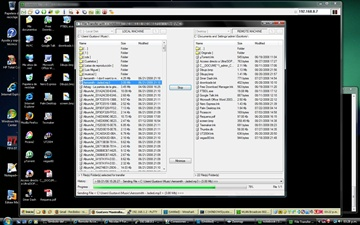
\includegraphics{imagenes/host-host/vnc_server}
	\caption{Sesi�n de UltraVNC a trav�s del enlace VPN con PPTP.}
	\label{fig:pptp_vnc_server}
	\end{center}
\end{figure}

\subsection{Transferencia de archivos}

Para la transferencia de archivos usando los sistemas Windows como se han descripto anteriormente, se procede de la manera tradicional, como si de una red local se tratara, es decir, compartiendo archivos mediante el protocolo SMB de Microsoft. La Figura \ref{fig:transferencia_host_to_host} muestra la tasa de transferencia medida en Bytes por segundos de un archivo de m�sica con compresi�n mpeg-layer3.

\begin{figure}[htb]
	\begin{center}
	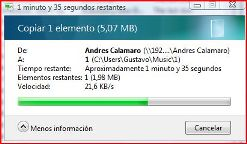
\includegraphics{imagenes/host-host/copia_hosthost}
	\caption{Transferencia de un archivo, a trav�s de la VPN host a host.}
	\label{fig:transferencia_host_to_host}
	\end{center}
\end{figure}

\subsection{Registro de conexiones}

Para realizar el registro de conexiones y verificar que el tr�fico de informaci�n se realiza de forma segura, se recurre a herramientas que monitorean el tr�fico de datos de una interfaz de red determinada. En el servidor y cliente se ha utilizado el software \texttt{Wireshark} antes y despu�s de establecer la conexi�n y transferir datos, con una salida similar a la que se muestra en el Registro \ref{logs:transferencia_host_to_host}.

\begin{logs}
  \begin{alltt}
  \scriptsize
  Source       Destination  Protocol Info
  200.45.35.51 192.168.0.35 TCP      scanstat-1 > pptp [SYN] Seq=0 Win=65535 Len=0 MSS=1440
  192.168.0.35 200.45.35.51 TCP      pptp > scanstat-1 [SYN, ACK] Seq=0 Ack=1 Win=8192 Len=0 MSS=1460
  200.45.35.51 192.168.0.35 PPTP     Start-Control-Connection-Request
  192.168.0.35 200.45.35.51 PPTP     Start-Control-Connection-Reply
  200.45.35.51 192.168.0.35 PPTP     Outgoing-Call-Request
  192.168.0.35 200.45.35.51 PPTP     Outgoing-Call-Reply
  200.45.35.51 192.168.0.35 PPTP     Set-Link-Info
  200.45.35.51 192.168.0.35 PPP LCP  Configuration Request
  192.168.0.35 200.45.35.51 PPP LCP  Configuration Request
  192.168.0.35 200.45.35.51 PPP LCP  Configuration Ack
  200.45.35.51 192.168.0.35 PPP LCP  Configuration Reject
  192.168.0.35 200.45.35.51 PPP LCP  Configuration Request
  200.45.35.51 192.168.0.35 PPP LCP  Configuration Ack
  192.168.0.35 200.45.35.51 PPTP     Set-Link-Info
  200.45.35.51 192.168.0.35 PPP LCP  Identification
  192.168.0.35 200.45.35.51 PPP CHAP Challenge (NAME='NIPPUR', VALUE=0x515E1AE701 ... )
  200.45.35.51 192.168.0.35 PPTP     Set-Link-Info
  200.45.35.51 192.168.0.35 PPP CHAP Response (NAME='remoto', VALUE=0xDFA67872B6F ... )
  192.168.0.35 200.45.35.51 GRE      Encapsulated PPP
  192.168.0.35 200.45.35.51 TCP      pptp > scanstat-1 [ACK] Seq=213 Ack=373 Win=64584 Len=0
  192.168.0.35 200.45.35.51 PPP CHAP Success (MESSAGE='S=817B882E753E7CC2732C41D78E34FAD05D59C59B')
  192.168.0.35 200.45.35.51 PPP CBCP Callback Request
  200.45.35.51 192.168.0.35 PPP CBCP Callback Response
  192.168.0.35 200.45.35.51 PPP CBCP Callback Ack
  200.45.35.51 192.168.0.35 PPP CCP  Configuration Request
  200.45.35.51 192.168.0.35 PPP IPCP Configuration Request
  192.168.0.35 200.45.35.51 GRE      Encapsulated PPP
  192.168.0.35 200.45.35.51 PPP CCP  Configuration Request
  192.168.0.35 200.45.35.51 PPP IPCP Configuration Request
  192.168.0.35 200.45.35.51 GRE      Encapsulated PPP
  200.45.35.51 192.168.0.35 PPP Comp Compressed data
  192.168.0.35 200.45.35.51 GRE      Encapsulated PPP
  ...
  \end{alltt}
  \caption{Establecimiento de la conexi�n host a host.}
  \label{logs:transferencia_host_to_host}
\end{logs}

Cuando se ha experimentado error en la conexi�n, como se puede observar en el Registro \ref{logs:error_host_to_host}, se debe a la mala configuraci�n de los firewall en ambos extremos, de manera que si el cliente se conectaba al servidor, este �ltimo no pod�a devolver el recibo de conexi�n al cliente, por lo que este nunca se enteraba si el servidor hab�a aceptado su petici�n.

Tambi�n se puede observar que si no se utilizara PPTP para transferir la informaci�n, y en alguno de los casos se env�a texto plano, el programa Wireshark mostrar�a el texto tal cual, aunque sea una contrase�a o n�mero de tarjeta de cr�dito. Por esto la importancia de utilizar PPTP a la hora de enviar informaci�n sensible, de forma r�pida y segura entre dos equipos.

\begin{logs}
  \begin{alltt}
	\scriptsize
  Source        Destination   Protocol Info
  192.168.0.35  200.45.153.14 TCP      62944 > pptp [SYN] Seq=0 Win=8192 Len=0 MSS=1460
  200.45.153.14 192.168.0.35  TCP      pptp > 62944 [SYN, ACK] Seq=0 Ack=1 Win=65535 Len=0 MSS=1440
  192.168.0.35  200.45.153.14 TCP      62944 > pptp [ACK] Seq=1 Ack=1 Win=64800 Len=0
  192.168.0.35  200.45.153.14 PPTP     Start-Control-Connection-Request
  200.45.153.14 192.168.0.35  PPTP     Start-Control-Connection-Reply
  192.168.0.35  200.45.153.14 PPTP     Outgoing-Call-Request
  200.45.153.14 192.168.0.35  PPTP     Outgoing-Call-Reply
  192.168.0.35  200.45.153.14 PPTP     Set-Link-Info
  192.168.0.35  200.45.153.14 PPP LCP  Configuration Request
  200.45.153.14 192.168.0.35  TCP      pptp > 62944 [ACK] Seq=189 Ack=349 Win=65187 Len=0
  192.168.0.35  200.45.153.14 PPP LCP  Configuration Request
  192.168.0.35  200.45.153.14 PPP LCP  Configuration Request
  192.168.0.35  200.45.153.14 PPP LCP  Configuration Request
  192.168.0.35  200.45.153.14 PPTP     Call-Clear-Request
  192.168.0.35  200.45.153.14 PPTP     [TCP Retransmission] Call-Clear-Request
  ...  
  \end{alltt}
  \caption{Error al establecer una conexi�n.}
  \label{logs:error_host_to_host}
\end{logs}

\section{Conclusi�n}
\label{sec:pptp_conclusion}

PPTP es un protocolo que lleva muchos a�os funcionando en sistemas Windows, y debido a la gran cantidad de usuarios que realizaron pruebas de seguridad y rendimiento, han terminado por decantar poco a poco su utilizaci�n en entornos de producci�n. A�n as�, se sigue utilizando en gran medida para conexiones simples de tipo host a red (entre equipos hogare�os principalmente), y hasta ha sido portado a sistemas libres (o de c�digo abierto) para su interacci�n con m�ltiples plataformas.

Esto refleja que, a pesar de todos los problemas de seguridad que ten�a el protocolo en la primera versi�n (que han sido solucionados parcialmente en la segunda versi�n), todav�a existe una gran cantidad de usuarios m�viles que se conectan a la red corporativa por PPTP mediante servidores Windows, Linux, BSD, Solaris, entre otros, sin importar la plataforma.

Por esta raz�n es que el protocolo deb�a ser probado y configurado para ambos sistemas, concluyendo que lo m�s dif�cil de esta implementaci�n ha sido la configuraci�n del firewall de la red local y del establecimiento de un ruteo adecuado.

La pol�tica de seguridad para los usuarios m�viles es hoy en d�a un tema de gran importancia, ya que se debe evitar que al extraviar el equipo personal, la red corporativa se vea comprometida. Esto se soluciona con el uso de usuarios y contrase�as no almacenados en el sistema y evitar tener certificados que se auto conecten al servidor de la empresa. A�n as�, este es un apartado importante para tener en cuenta cuando se crean las pol�ticas de seguridad y la infraestructura de la red.

Finalmente se puede recalcar que PPTP se va a seguir usando por mucho tiempo m�s, debido al soporte que existe en varias plataformas y a la gran cantidad de usuarios que tiene, como se ha mencionado anteriormente. Adem�s, los equipos port�til vienen con sistemas Windows que tienen por defecto implementado el protocolo PPTP, lo hacen ideal para las empresas con empleados que viajan con frecuencia, ya que no requieren de instalar ning�n software adicional.


%% VPN con SSH/PPP
%%%%%%%%%%%%%%%%%%%%%%%%%%%%%%%%%%%%%%%%%%%%%%%%%%%%%%%%
%   |-------------------------|                        %
%   |REDES PRIVADAS VIRTUALES |                        %
%   |                         |                        %
%   | Proyecto de graduaci�n  |                        %
%   |_________________________|                        %
%                                                      %
%   Autores                                            %
%   -------                                            %
%                                                      %
% * Formoso Requena, Nicol�s Federico (CX02-0239-8)    %
%     nicolasformoso@gmail.com                         %
% * Cortez, Gustavo Maximiliano (CX01-0801-9)          %
%     cmgustavo83@gmail.com                            %
%                                                      %
%   Tutores                                            %
%   -------                                            %
%                                                      %
% * Ing. Gustavo Vanetta - vanettag@gmail.com          %
% * Lic. Miguel Bazzano - miguelbazzano@gmail.com      %
%                                                      %
%%%%%%%%%%%%%%%%%%%%%%%%%%%%%%%%%%%%%%%%%%%%%%%%%%%%%%%%

% ************* VPN usando PPP sobre SSH ************* %

\chapter{VPN usando PPP sobre SSH}
\label{chap:vpn_pppsobressh}

En este cap�tulo se describir� un modo de establecer una VPN entre dos redes distantes de forma segura. Para esto se utiliza el protocolo PPP y la herramienta SSH, de las cuales se dar�n una breve introducci�n te�rica.

Adem�s se detallar�n los procesos de creaci�n y distribuci�n de las claves utilizadas para ingresar en el sistema mediante SSH, la configuraci�n de ruteo y del firewall de cada red.

\section{Protocolo PPP}
\label{sec:proto_ppp}

El protocolo \gls{PPP} permite establecer una comunicaci�n a nivel de enlace entre dos computadoras. Utilizado com�nmente para establecer la conexi�n a Internet de un particular con su proveedor de acceso a trav�s de un m�dem telef�nico. Tambi�n utilizado sobre conexiones de banda ancha (como PPPoE o PPPoA). Adem�s del simple transporte de datos, PPP facilita dos funciones importantes:

\begin{itemize}
\item Autenticaci�n. Generalmente mediante una clave de acceso (que en nuestro caso no ser� necesario).
\item Asignaci�n din�mica de IP. Los proveedores de acceso cuentan con un n�mero limitado de direcciones IP y cuentan con m�s clientes que direcciones. Naturalmente, no todos los clientes se conectan al mismo tiempo. As�, es posible asignar una direcci�n IP a cada cliente en el momento en que se conectan al proveedor. La direcci�n IP se conserva hasta que termina la conexi�n por PPP. Posteriormente, puede ser asignada a otro cliente.
\end{itemize}

PPP soporta, entre otros, los tipos de autenticaci�n PAP y CHAP. La primera, es la m�s insegura, ya que env�a nuestro usuario y contrase�a en texto claro a trav�s de la red; la segunda encripta estos datos, para que no puedan ser le�dos.

Una gran desventaja de este protocolo, es que no proporciona cifrado de datos, por lo que todo el flujo de informaci�n de una conexi�n PPP es enviada en claro, de modo que si alguien est� capturando los paquetes transmitidos, puede leer toda la carga que se env�a y recibe, teniendo acceso a nuestra informaci�n privada.

\section{Protocolo y aplicaci�n SSH}
\label{sec:proto_ssh}

\gls{SSH} o \emph{int�rprete de comandos seguro} es el nombre de un protocolo y el programa que lo implementa. Sirve para acceder a m�quinas remotas a trav�s de una red. Permite manejar por completo la computadora mediante un int�rprete de comandos, y tambi�n puede redirigir el tr�fico de X para poder ejecutar programas gr�ficos si se tiene un Servidor X\footnote{Sistema gr�fico utilizado en sistemas Unix}.

Adem�s de la conexi�n a otras m�quinas, SSH permite copiar datos de forma segura (tanto archivos sueltos como simular sesiones FTP cifradas), gestionar claves RSA para no escribir claves al conectar a las m�quinas y pasar los datos de cualquier otra aplicaci�n por un canal seguro tunelizado mediante SSH.

La primera versi�n del protocolo y el programa eran libres, pero su licencia fue cambiando y termin� apareciendo la compa��a SSH Communications Security, que lo ofrec�a gratuitamente para uso dom�stico y acad�mico, pero exig�a el pago a otras empresas.

La implementaci�n libre por excelencia, llamada \emph{OpenSSH}, es la que se va a utilizar en este proyecto; debido a que -seg�n sus desarrolladores (los mismos que desarrollaron OpenBSD)- es m�s segura que la original.

\subsection{Seguridad}

SSH trabaja de forma similar a como se hace con telnet. La diferencia principal es que SSH usa t�cnicas de cifrado que hacen que la informaci�n que viaja por el medio de comunicaci�n vaya de manera no legible y ninguna tercera persona pueda descubrir el usuario y contrase�a de la conexi�n ni lo que se escribe durante toda la sesi�n.

\section{Descripci�n General de la VPN}

La topolog�a seleccionada para esta implementaci�n, es de red a red; esto nos permite hacer que las redes locales involucradas tengan la impresi�n de que est�n unidas simplemente por un router, mientras que en realidad, puede que se encuentren a kil�metros de distancia. La Figura \ref{fig:vpn_detras_fw} muestra las dos redes, y la VPN establecida entre ellas. 

En cada una de las subredes hay un solo punto de entrada/salida a Internet, donde se implementa el firewall. Detr�s de este se encuentra toda la red local, y el Servidor VPN, que puede definir sus propias reglas de filtrado de paquetes para sus conexiones.

Todo el flujo de datos que se dirige a Internet, va directo por la puerta de enlace; los paquetes que pertenecen a la conexi�n VPN, se dirigen primero al servidor VPN, para luego salir por la puerta de enlace.

En la realidad, para este modo de establecer una VPN, no se utiliza ning�n protocolo espec�fico para redes privadas virtuales. A lo que se denomina servidor VPN, y cliente VPN \textendash en este caso\textendash, en realidad ser�an el servidor SSH y el cliente SSH, ya que este es el protocolo que establece la conexi�n entre ambos puntos.

Los servidores VPN se implementan sobre \emph{GNU/Linux Ubuntu Server 8.04}. Para saber m�s detalles sobre las redes que se utilizaron para las pruebas, v�ase el Ap�ndice \ref{appendix:equipos_de_prueba}. 

\begin{figure}[htbp]
\centering
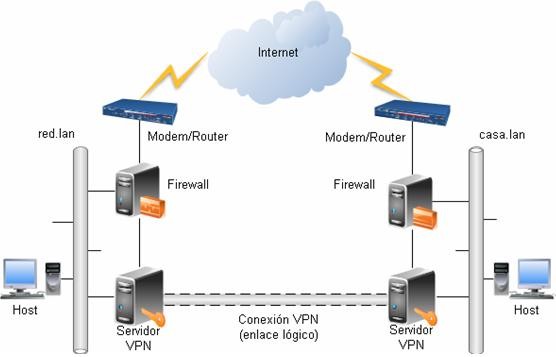
\includegraphics{imagenes/red-red/vpn_detras_fw}
\caption{Servidor VPN detr�s del Firewall}
\label{fig:vpn_detras_fw}
\end{figure}

\section{Funcionamiento}

El servidor VPN (ubicado en la red \emph{casa.lan}), espera conexiones SSH en un puerto distinto al 22 \textendash que es el est�ndar para este protocolo\textendash, tomado para evitar que se mezclen los paquetes SSH de las Shells est�ndar, con los de las conexiones VPN; esto, a fines de un mayor control sobre qui�n se conecta a la red local.

Debido a que este servidor se encuentra detr�s del firewall/puerta de enlace, se debe hacer una redirecci�n hacia dicho servidor, de todos los paquetes que quieran entrar o salir por el puerto en el que se est�n escuchando las conexiones VPN.

Por su parte, el cliente (ubicado en la red \emph{red.lan}) que desea efectuar una conexi�n VPN, debe utilizar los protocolos ppp y ssh, para lograrlo.

En la puerta de enlace de la red cliente, no es necesario hacer ning�n cambio adicional (a nivel de reglas de firewall, redireccionamiento o nat) para que funcione esta VPN.

Cuando se establece la conexi�n, en ambos servidores se crea una nueva interfaz, por ejemplo \emph{ppp0}, a trav�s de la cual se env�a y recibe el flujo de datos de la red contraria. A esta interfaz se asocia una direcci�n IP; para esto se ha elegido \texttt{192.168.254.1} para el servidor, \texttt{192.168.254.2} para el cliente. La m�scara de subred de estas direcciones es \texttt{255.255.255.255}, por lo que pueden crearse cuantos pares de direcciones se deseen para distintas VPN, siempre que no haya solapamiento.

Vale aclarar, que las denominaciones cliente y servidor VPN, cobran sentido solo para el establecimiento de la conexi�n, ya que solo el cliente puede solicitarlo. Cuando la conexi�n est� establecida, los datos pueden requerirse indistintamente de una red, como de la otra; no existe jerarqu�a entre ellos. Es por este motivo se llama \emph{servidor VPN} tambi�n al cliente.

\subsubsection{El enrutamiento}

El establecimiento de las rutas, luego de la conexi�n, es importante para que las redes puedan traficar datos entre ellas; de otro modo, por m�s que la conexi�n est� establecida, no podr�n compartir informaci�n.

Hay m�s de una forma de definir las rutas entre las redes, pero no todas permiten que la VPN sea transparente, ya que requieren modificaciones en los terminales de usuarios. En este caso se requiere que en los hosts internos no tengan que agregar o quitar nada para que la conexi�n VPN funcione, por lo tanto, se establecen las rutas solo en el servidor VPN y en la puerta de enlace. Esta situaci�n se ve reflejada en la Figura \ref{fig:vpn_detras_fw}.

Suponiendo que la puerta de enlace predeterminada en \emph{casa.lan} tiene la direcci�n \texttt{192.168.1.2} y el Servidor VPN \texttt{192.168.1.3}. Del otro lado, en \emph{red.lan}, el gateway por defecto tiene la direcci�n \texttt{192.168.0.1} y el servidor VPN \texttt{192.168.0.2}.

De esta manera se pretende que los hosts de las redes se vean entre s�, es decir, que cuando el nodo \texttt{192.168.0.20} quiera conectarse con \texttt{192.168.1.7} (aunque est�n en redes diferentes) pueda hacerlo sin modificaci�n alguna de sus rutas. Por esto, se debe establecer en la puerta de enlace de \emph{casa.lan} que cuando llegue un paquete dirigido a la red \texttt{192.168.0.0/24} lo env�e al servidor VPN local, ya que este conoce la ruta. Se puede hacer mediante el siguiente comando (como superusuario):

\begin{verbatim}
# route add 192.168.0.0/24 192.168.1.3
\end{verbatim}

La puerta de enlace enviar� al servidor VPN todos los paquetes que tienen como destino la red contraria, por lo tanto, se debe especificar por d�nde deber�n llegar a la misma. Cuando se ha establecido la conexi�n VPN, se ha creado en cada servidor, una nueva interfaz llamada \emph{ppp0}, asociada a una direcci�n IP. Esta interfaz es la que comunica una red con la otra a trav�s del t�nel SSH, y en la red \emph{casa.lan} tiene la direcci�n \texttt{192.168.254.1}. Con la siguiente l�nea todos los paquetes que llegue al servidor con destino la red \texttt{192.168.0.0/24} se enviar�n por la interfaz ppp0 a dicha red.

\begin{listing}[style=consola, numbers=none]
# route add -net 192.168.0.0/24 gw 192.168.254.1
\end{listing}

Ahora en \emph{red.lan}, se debe hacer lo mismo, es decir, en el gateway por defecto se agrega la direcci�n del servidor VPN:

\begin{listing}[style=consola, numbers=none]
# route add 192.168.1.0/24 192.168.0.2
\end{listing}

Y luego la ruta que lleva a la otra red por la interfaz ppp0:

\begin{listing}[style=consola, numbers=none]
# route add -net 192.168.1.0/24 gw 192.168.254.2
\end{listing}

N�tese que la sintaxis del comando ``route'' var�a entre las puertas de enlace y en los servidores VPN, esto se debe a que poseen sistemas operativos distintos: OpenBSD y GNU/Linux respectivamente. En cada caso, ver la p�gina del manual para m�s informaci�n \cite{man}.

\subsection{Env�o y recepci�n de paquetes}

Si se tiene una VPN establecida entre el cliente y el servidor mencionados anteriormente, y ahora el host \texttt{192.168.0.20} de la red \emph{red.lan} desea probar si el host \texttt{192.168.1.7} se encuentra activo, se ejecuta el comando \texttt{ping 192.168.1.7}, que env�a paquetes \emph{ICMP Echo Request} al destino especificado, y este �ltimo responder� con paquetes \emph{ICMP Echo Replay} para notificar al origen positivamente. 

El host \texttt{192.168.0.20} tiene configurado en su tabla de ruteo solamente el gateway por defecto, por lo que al ejecutar el comando \texttt{ping 192.168.1.7} y no encontrar en la tabla una ruta directa hacia la red \texttt{192.168.1.0/24} (o a dicho host), env�a los paquetes por la ruta predeterminada.

Esta ruta predeterminada es la puerta de enlace al mundo exterior, la que deber� conocer el camino hacia la red \texttt{192.168.1.0/24}, y que no es precisamente enviando los paquetes a trav�s de Internet \textendash ya que son direcciones de una red privada \textendash, sino envi�ndolos al servidor VPN. Por lo tanto, el gateway por defecto debe tener expl�citamente una ruta hacia el la red contraria.

Cuando los paquetes ICMP Echo Request enviados por el host \texttt{192.168.0.20} llegan al servidor VPN de la red, este conoce el camino hacia la otra red: a trav�s de la interfaz \emph{ppp0} mencionada anteriormente, y que es el enlace PPP encapsulado en la conexi�n SSH.

Por lo tanto, lo que el servidor hace, es a�adir a los paquetes ICMP Echo Request las correspondientes cabeceras PPP (que son de nivel de enlace de datos), donde se encuentra la direcci�n IP destino (asociada con la interfaz ppp0).

Estas tramas PPP son encapsuladas en paquetes SSH, cuya direcci�n origen es el servidor VPN (la direcci�n local), y direcci�n destino la direcci�n p�blica de la red donde se encuentra el servidor VPN destino.

Cuando los paquetes llegan a la puerta de enlace de la red destino, este los env�a al servidor VPN local, analiza el contenido y lo env�a al host destino.

Para que la VPN sea realmente transparente a los usuarios finales de cada red, el encaminamiento es un punto muy importante. En la Figura \ref{fig:resultado_redared} se muestra el diagrama de red que los hosts percibir�n luego de establecer la conexi�n VPN.

\begin{figure}[htbp]
\centering
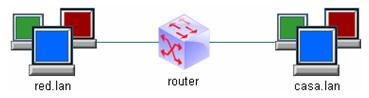
\includegraphics{imagenes/red-red/resultado_redared}
\caption{Luego del establecimiento de la VPN Red a Red}
\label{fig:resultado_redared}
\end{figure}

El esquema de direcciones de \emph{red.lan} es \texttt{192.168.0.0/24} y el de \emph{casa.lan} es \texttt{192.168.1.0/24}; a partir de la Figura \ref{fig:resultado_redared}, si el usuario \texttt{192.168.0.20} ejecuta el comando \texttt{ping 192.168.1.7} \textendash y los caminos en el router est�n bien configurados \textendash, el host \texttt{192.168.0.20} deber�a recibir la respuesta de sus ICMP ECHO REQUESTs del host solicitado.

\section{Configuraci�n del Servidor VPN}
\label{sec:pppssh_configuracion_servidor}

Es importante ser cauteloso a la hora de configurar un servicio que se brindar� hacia afuera, ya que no hay que dejar huecos o puertas traseras que puedan ser utilizadas para introducirse en el sistema local, y poner en riesgo a toda red.

La ventaja de utilizar como servidor VPN un sistema derivado de Unix \textendash GNU/Linux en este caso \textendash es que son muy flexibles en lo que se refiere a configuraci�n de seguridad, y est�n (desde su concepci�n) dotados de varias capas de seguridad, y preparados para funcionar como verdaderos servidores.

En esta secci�n se describir� c�mo poner a punto el servidor VPN, con un grado de seguridad m�s elevado.

\subsection{Directivas de firewall}

Como se ha mencionado anteriormente, el servidor VPN escuchar� las conexiones SSH que ingresen por el puerto 9876. Pero debido a que dicho servidor se encuentra detr�s del firewall, esta escucha se limita a la red local. Para que se pueda escuchar incluso las conexiones que provengan desde internet, se debe redireccionar en el firewall a dicho puerto. 

Esto se logra agregando una l�nea en el archivo de configuraci�n del firewall, como se muestra en la Configuraci�n \ref{config:pf.conf.sshppp}.

\begin{configuracion}
\begin{listing}[style=configuracion]
rdr pass on $ext_if proto tcp from any to any port 9876 -> $server_vpn
\end{listing}
\caption{L�neas en el archivo \texttt{/etc/pf.conf}}
\label{config:pf.conf.sshppp}
\end{configuracion}

De la Configuraci�n \ref{config:pf.conf.sshppp}, \$ext\_if es la interfaz conectada al proveedor de internet, y \$server\_vpn es define la direcci�n IP de dicho servdidor.

Para refrescar las directivas del Packet Filter sin tener que reiniciar el equipo se ejecuta el siguiente comando:

\begin{listing}[style=consola, numbers=none]
$ sudo pfctl -f /etc/pf.conf
$
\end{listing}

\subsection{Activando el Port Forwarding}

Para poder recibir conexiones desde el exterior de la red, es decir, para que un ordenador remoto pueda conectarse con el servidor VPN interno de la red, se debe activar el \emph{port forwarding}, con el siguiente comando:

\begin{listing}[style=consola, numbers=none]
$ sudo /sbin/sysctl -w net.ipv4.ip_forward=1
$
\end{listing}

Para que se accione cada vez que se inicia el equipo, se debe agregar la siguiente l�nea en el archivo \texttt{/etc/sysctl.conf}:

\begin{verbatim}
net.ipv4.ip_forward=1
\end{verbatim}

\subsection{Creando un nuevo usuario}
\label{subsec:crear_user_enserver}

Cuando el cliente VPN\footnote{El servidor VPN que act�a como cliente al momento de la conexi�n} intenta establecer la conexi�n, debe conectarse a trav�s de SSH al servidor VPN y levantar el demonio PPPD; para estos fines es que se crea un nuevo usuario del lado del servidor. Este usuario estar� restringido en casi todo aspecto.

Antes de crear el usuario, se crea un grupo para el mismo de igual nombre:

\begin{listing}[style=consola, numbers=none]
$ sudo addgroup sshvpn
$ sudo adduser --home /home/sshvpn --ingroup sshvpn --disabled-login sshvpn
\end{listing}

N�tese que ambas l�neas comienzan con \emph{sudo}, este comando se utiliza para que un usuario que no posee privilegios de administrador, pero si permiso para ejecutar comandos que requieren estos privilegios, a trav�s de este programa, pueda hacerlo. Por ejemplo, los comandos \emph{addgroup} y \emph{adduser} solo pueden ser ejecutados por el usuario administrador, y por quienes hayan sido autorizados para hacerlo a trav�s del comando \emph{sudo}. (Ver m�s detalles en \cite{man}).

La primera l�nea, sencillamente lo que hace es a�adir un nuevo grupo al sistema, llamado \emph{sshvpn}.

La segunda l�nea a�ade nuestro usuario. Este tendr� como directorio de trabajo \emph{/home/sshvpn}; como grupo \emph{sshvpn}; no podr� ser accedido directamente como una cuenta local, por lo que no poseer� password (\emph{--disabled-login}), y su nombre ser� \emph{sshvpn}.

\subsection{Configuraci�n de \emph{sudo}}
\label{subsec:conf_sudo_enserver}

El nuevo usuario del servidor, debe ser capaz de levantar el demonio \texttt{pppd}, a fines de establecer la conexi�n. Como los demonios solo pueden ser ejecutados por el administrador, se deben dar permiso a nuestro usuario para que lo haga a trav�s del programa \emph{sudo}, sin darle permisos de superusuario. Para modificar la configuraci�n del sudo, debe editarse el archivo \texttt{/etc/sudoers} (m�s detalles en \cite{man}), con el programa \texttt{visudo}, y se agrega la l�nea:

\begin{verbatim}
sshvpn ALL=NOPASSWD: /usr/sbin/pppd
\end{verbatim}

Luego el usuario \emph{sshvpn} ya tiene permisos para ejecutar el demonio \emph{pppd}, y sin necesidad de introducir una contrase�a. Esto es importante ya que se pretende que la conexi�n se establezca autom�ticamente por s� misma, con la menor (o nula) intervenci�n posible de una persona. En Linux, el demonio \emph{pppd} est� ubicado en /usr/sbin, pero esto puede variar en otras distribuciones.

Cabe aclarar que el hecho de que sshvpn tenga la posibilidad de levantar un demonio sin ser administrador, no va en desmedro de la seguridad, lo cual ser� aclarado a medida que se vayan analizando la configuraciones.

\subsection{Aceptando conexiones SSH provenientes del cliente}
\label{sec:aceptando_ssh}

El protocolo SSH tiene la posibilidad de establecer conexiones entre hosts sin necesidad de introducir contrase�as de modo interactivo, gracias a un sistema de claves que permite al servidor reconocer de forma un�voca al cliente.

En este se deben generar un par de claves asim�tricas RSA (v�ase Secci�n \ref{sec:generando_claves}), la clave privada permanece en el cliente, y la clave p�blica la debemos llevar al servidor VPN. Supongamos que nuestra clave p�blica est� en un archivo llamado \emph{id\_rsa\_key\_cliente.pub}.

Ahora debemos permitir las conexiones a trav�s de SSH para el usuario sshvpn, de la siguiente forma:

\begin{listing}[style=consola, numbers=none]
# cd /home/sshvpn
# mkdir .ssh/
# cd .ssh/
# mv /camino/a/id_rsa_key_cliente.pub .
# cat id_rsa_key_cliente.pub >> authorized_keys
\end{listing}

El archivo \emph{/home/sshvpn/.ssh/authorized\_keys} contiene todas las claves p�blicas de los distintos clientes que est�n permitidos ingresar al sistema como este usuario. Luego de esto, el cliente podr� ingresar al servidor VPN, sin necesidad de contrase�a, �nicamente con el comando \emph{ssh el.servidor.com.ar}.

\subsection{Lanzando un nuevo demonio SSH}

Como se ha mencionado anteriormente, no se va a utilizar el mismo puerto para conectar las shells SSH y la VPN. Por lo tanto se ejecutar� otro demonio SSH, configurado para que escuche en un puerto espec�fico, y para que solo sean aceptados los que desean establecer una VPN.

N�tese que esta es una de las capas de seguridad. Se esta denegando el acceso por el puerto determinado a los usuarios que no tienen permisos para establecer una conexi�n VPN.

\emph{sshd} al ejecutarse, lee un archivo de configuraci�n generalmente \texttt{/etc/ssh/sshd\_config}. Como no se pretende modificar las opciones del demonio que escucha por el puerto 22, no se modifica ese archivo. Se Crea un nuevo archivo de configuraci�n y se lo ubica en \texttt{/home/sshvpn/etc/}, con el nombre \texttt{sshppp\_config}, que se muestra en la Configuraci�n \ref{config:sshppp_config}.

\begin{configuracion_small}
\begin{listing}[style=configuracion_small]
PidFile /var/run/sshvpn.pid
Port 9876
Protocol 2

HostKey /etc/ssh/ssh_host_rsa_key
HostKey /etc/ssh/ssh_host_dsa_key

#Privilege Separation is turned on for security
UsePrivilegeSeparation yes

# Lifetime and size of ephemeral version 1 server key
KeyRegenerationInterval 3600
ServerKeyBits 768

# Logging
SyslogFacility AUTH
LogLevel INFO

# Authentication:
LoginGraceTime 120
PermitRootLogin no
StrictModes yes

RSAAuthentication yes
PubkeyAuthentication yes

AllowUsers sshvpn

#AuthorizedKeysFile	%h/.ssh/authorized_keys
IgnoreRhosts yes
RhostsRSAAuthentication no
HostbasedAuthentication no
PermitEmptyPasswords no
ChallengeResponseAuthentication no
PasswordAuthentication yes

X11Forwarding no
X11DisplayOffset 10
PrintMotd no
PrintLastLog yes
TCPKeepAlive yes

Subsystem sftp /usr/lib/openssh/sftp-server
UsePAM yes
\end{listing}
\caption{Archivo /home/sshvpn/etc/sshppp\_config.}
\label{config:sshppp_config}
\end{configuracion_small}

Lo m�s importante que se puede destacar de \ref{config:sshppp_config}, son las primeras opciones en la que el archivo PID del demonio ser� \texttt{/var/run/sshvpn.pid}. El puerto en el que escuchar� es el 9876 y el protocolo SSH utilizado es la versi�n 2.

Tambi�n es importante notar la opci�n \emph{AllowUsers sshvpn}. Esto permite que solo pueda ingresar por este puerto el usuario sshvpn, y ning�n otro.

Todas las dem�s opciones son restricciones de seguridad para evitar ingresos no deseados; a estas se las puede encontrar en la p�gina del manual del archivo en \cite{man}.

Para lanzar el demonio, solo basta ejecutar como superusuario el comando: 

\begin{listing}[style=consola, numbers=none]
# /sbin/sshd -f /home/sshvpn/etc/sshppp_config
\end{listing}

\section{Configuraci�n del Cliente VPN}
\label{sec:pppssh_configuracion_cliente}

En esta secci�n se detallan los pasos necesarios para configurar el extremo cliente de una conexi�n PPP y SSH. Lo par�metros van desde la creaci�n del usuario �nico permitido para conectarse con el servidor, hasta la definici�n de los alias de red, pasando por la generaci�n de claves RSA y una muestra de la conexi�n realizada. 

\subsection{Creando un nuevo usuario}

En el cliente VPN tambi�n se crea un usuario que ser� el encargado de establecer la conexi�n VPN con el servidor, y a efectos de simplicidad, este usuario tendr� el mismo nombre que el usuario creado en el servidor.

Antes de crear el usuario, se crea un grupo con el mismo nombre de la siguiente manera:

\begin{listing}[style=consola, numbers=none]
$ sudo addgroup sshvpn
$ sudo adduser --home /home/sshvpn --ingroup sshvpn sshvpn
$ sudo passwd sshvpn
$
\end{listing}

Esto es similar a lo que se hace en el servidor (Secci�n \ref{subsec:crear_user_enserver}). La diferencia es que aqu� es necesario acceder al usuario sshvpn, por lo que se omite la opci�n \texttt{--disable-login} en la creaci�n del usuario.

Con el comando \emph{passwd sshvpn} se establece una contrase�a para poder ingresar como usuario \texttt{sshvpn}.

\subsection{Generando las claves RSA}
\label{sec:generando_claves}

Ahora es necesario generar el par de claves p�blica/privada en el cliente; guardar la privada y pasar al servidor la clave p�blica para poder acceder a �l sin necesidad de contrase�a. Esto se hace de la siguiente forma:

\begin{listing}[style=consola, numbers=none]
# su - sshvpn
# mkdir .ssh/
# cd .ssh/
# ssh-keygen -t rsa -N ''
\end{listing}

Primero se debe cambiar al usuario sshvpn (con el comando ``su - sshvpn''); luego en el directorio \texttt{.ssh} se generan las claves con el comando \emph{ssh-keygen}. Los archivos generados son \texttt{id\_rsa} (la clave privada que se guarda en el cliente) e \texttt{id\_rsa.pub} (la clave p�blica que se env�a al servidor, v�ase Secci�n \ref{sec:aceptando_ssh}). Para enviarla, se escribe lo siguiente (utilizando \gls{SCP}):

\begin{listing}[style=consola, numbers=none]
# scp ./id_rsa.pub sshvpn@el.servidor.com.ar:/home/sshvpn/.ssh/id_rsa_key_cliente.pub
\end{listing}

\subsection{Configuraci�n de sudo}

Como este paso se realiza de la misma manera que en \ref{subsec:conf_sudo_enserver}), solamente se mostrar� la l�nea que se debe agregar con \texttt{visudo}:

\begin{verbatim}
sshvpn ALL=NOPASSWD: /usr/sbin/pppd
\end{verbatim}

En el cliente tambi�n es necesario que el usuario sshvpn pueda levantar el demonio \texttt{pppd}, para que se pueda establecer las conexi�n.

\subsection{Conectando al Servidor}

La conexi�n al servidor se efect�a desde el cliente con una simple l�nea ejecutada como el nuevo usuario sshvpn que se a creado anteriormente. El comando es el siguiente \footnote{La barra invertida (\textbackslash)en el comando indica corte de l�nea}:

\begin{verbatim}
sudo /usr/sbin/pppd updetach noauth pty "sudo -u sshvpn ssh -p 9876 -t -t servidor \
		sudo /usr/sbin/pppd noauth 192.168.254.1:192.168.254.2"
\end{verbatim}

Como sshvpn debe ejecutar el demonio \texttt{pppd} a trav�s del comando sudo, se ejecuta dicho demonio con las siguientes opciones:

\begin{itemize}
	\item \emph{updetach}: Desvincula a pppd de la terminal donde se lo ejecuta, para que pueda seguir us�ndose dicha terminal.
	\item \emph{noauth}: Como en este caso la autenticaci�n est� a cargo del protocolo SSH, no se necesita autenticar al momento de conectar \texttt{pppd}.
	\item \emph{pty ``...''}: Ejecuta el comando encerrado entre comillas antes de conectarse.
\end{itemize}

Luego se ejecuta el pppd local, antes de proceder a conectarse. Debido a que el primer \texttt{pppd} se ejecuta con sudo, el comando ssh dentro de pty ``...'', tambi�n se ejecutar�a con permisos del usuario raiz, y por lo tanto buscar�a el archivo \texttt{authorized\_keys} en el directorio \texttt{.ssh/} del directorio de root. 

Como se requiere que busque el directorio de sshvpn, lo que se hace es ejecutar el ssh como \texttt{sshvpn} mediante el comando: \emph{sudo -u sshvpn}.

A ssh se le pasan los siguientes par�metros:

\begin{itemize}
	\item \emph{-p 9876}: Especifica el puerto del servidor al que debe intentar conectarse.
	\item \emph{-t -t}: Obliga al otro extremo alojar en una \texttt{tty} (terminal del sistema) al comando que se ejecuta. Esto es necesario para ejecutar \texttt{pppd}.
	\item \emph{servidor}: Es el nombre de dominio del servidor al cual se va a conectar.
	\item \emph{sudo /usr/sbin/pppd noauth 192.168.254.1:192.168.254.2}: Esta l�nea se ejecuta en el servidor a trav�s de ssh. Lo que hace es levantar el demonio \texttt{pppd} en el servidor, con la opci�n \emph{noauth}, y otorg�ndole como par�metros las direcciones IP que utilizar�n el cliente y el servidor.
\end{itemize}

\subsection{Creando un alias para la VPN}

Con el objeto de simplificar un poco las cosas para el cliente, ssh permite crear \emph{aliases} para distintas conexiones; esto es, asociar a un nombre f�cil de recordar, un nombre de dominio, puerto, usuario, etc�tera.

El archivo que permite esto es \texttt{.ssh/config} del directorio personal de sshvpn, cuyo contenido se muestra en la Configuraci�n \ref{config:aliases_config}.

\begin{configuracion}
\begin{listing}[style=configuracion]
# Este archivo se encuentra en ~sshvpn/.ssh/
#
# UN ALIAS para la VPN ssh+ppp con el dominio nicolasformoso.com.ar
Host vpn_sshppp
Hostname nicolasformoso.com.ar
User sshvpn
Port 9876 
IdentityFile ~/.ssh/id_rsa
\end{listing}
\caption{Archivo /home/sshvpn/.ssh/config}
\label{config:aliases_config}
\end{configuracion}

A partir de ahora, cuando se escriba \emph{ssh vpn\_sshppp}, se establecer� una conexi�n SSH con el dominio \emph{nicolasformoso.com.ar}, por el puerto 9876 y con el usuario sshvpn. En este archivo pueden definirse tantos \emph{aliases} como se necesiten, en forma secuencial.

\section{A�adiendo seguridad a la VPN}
\label{sec:pppssh_seguridad}

En esta secci�n se mostrar�n consejos simples que hacen a la conexi�n VPN un poco m�s segura, ya sea restringiendo el acceso al servidor SSH, como limitando el uso de ciertos comandos que no son necesarios para establecer la conexi�n.

\subsection{Bloqueando la Shell de sshvpn}

Como no se pretende que el usuario sshvpn tenga acceso al servidor a trav�s de una shell, sino que solo pueda establecer la conexi�n VPN, se agrega antes de la clave p�blica lo siguiente:

\begin{verbatim}
command="sudo /usr/sbin/pppd noauth 192.168.254.1:192.168.254.2"
\end{verbatim}

De esta manera cuando sshvpn intente ingresar por el puerto 9876, lo �nico que podr� hacer es ejecutar \texttt{pppd}.

Ahora el comando para conectar con la VPN se simplifica, quedando:

\begin{listing}[style=consola, numbers=none]
$ sudo /usr/sbin/pppd updetach noauth pty "sudo -u sshvpn ssh vpn_sshppp"
$
\end{listing}

Donde \texttt{vpn\_sshppp} es el nombre del alias creado para la VPN en cuesti�n.

\subsection{Restringiendo las claves}

Si se tiene la posibilidad de conocer la direcci�n IP p�blica de la red donde se encuentra el cliente VPN, restringir el uso de una clave p�blica para esa direcci�n IP anteponiendo a la clave, es una buena opci�n para evitar el inconveniente del robo de claves.

\begin{verbatim}
from="direcci�n ip del cliente"
\end{verbatim}

\subsection{Otras opciones}

Para que no se pueda ingresar al servidor X, ni utilizar Agent Forwarding, se agrega a la clave:

\begin{verbatim}
no-X11-forwarding,no-agent-forwarding
\end{verbatim}

Existen otras opciones que tambi�n se pueden agregar en el archivo \texttt{authorized\_keys} que pueden obtenerse de \cite{man}; todas ellas deben ir separadas por una coma entre s�, y por un espacio en blanco de la clave.

Luego que se haya a�adido a las opciones del archivo \texttt{authorized\_keys}, se muestra en la Configuraci�n \ref{config:authorized_keys}.

\begin{configuracion_small}
\begin{listing}[style=configuracion]
command="sudo /usr/sbin/pppd noauth 192.168.254.1:192.168.254.2",no-X11-forwarding,no-agent-forwarding ssh-rsa AAAAB3NzaC1yc2EAAAABIwAAAQEAnpyZ5BiLj5Yb8bW3eLf7CwGR ... yRSvYfiIOdwHk+FFNp0JkStMEg4shVMXQ== sshvpn@notebook
\end{listing}
\caption{Archivo /home/sshvpn/.ssh/authorized\_keys}
\label{config:authorized_keys}
\end{configuracion_small}

\section{Conclusi�n}
\label{sec:pppssh_conclusion}

Para establecer una red privada virtual utilizando el conjunto de protocolos PPP y SSH, se tiene que contar con una configuraci�n muy bien detallada, porque sino se pueden generar agujeros de seguridad que implicar�an en accesos no autorizados a la red.

Esta tecnolog�a se la utiliza para la topolog�a red a red de una VPN, y a pesar de que se puede configurar para m�ltiples clientes, su complejidad puede llegar a ser tan alta que se tendr�a que buscar alternativas. Por esta raz�n es que se realizan conexiones punto a punto, en donde un servidor y cliente, cuentan con sus propias redes privadas. La idea es conectar dichas redes utilizando protocolos muy seguros y probados.

La combinaci�n de PPP y SSH permite utilizar los conceptos y archivos de configuraci�n ya conocidos de estos servicios para luego juntarlos y tener una infraestructura de red segura y estable. La dificultad de su configuraci�n y el tener en cuenta los detalles de seguridad en cuanto a las conexiones SSH y el puerto a utilizar, hacen que sea una opci�n algo complicada de llevar a la pr�ctica.

Pero a�n as�, con las rutas configuradas y los numerosos archivos involucrados, se puede tener un enlace red a red altamente seguro y en un tiempo razonable si ya se tiene experiencia previa.


%% VPN con IPSec
%%%%%%%%%%%%%%%%%%%%%%%%%%%%%%%%%%%%%%%%%%%%%%%%%%%%%%%%
%   |-------------------------|                        %
%   |REDES PRIVADAS VIRTUALES |                        %
%   |                         |                        %
%   | Proyecto de graduaci�n  |                        %
%   |_________________________|                        %
%                                                      %
%   Autores                                            %
%   -------                                            %
%                                                      %
% * Formoso Requena, Nicol�s Federico (CX02-0239-8)    %
%     nicolasformoso@gmail.com                         %
% * Cortez, Gustavo Maximiliano (CX01-0801-9)          %
%     cmgustavo83@gmail.com                            %
%                                                      %
%   Tutores                                            %
%   -------                                            %
%                                                      %
% * Ing. Gustavo Vanetta - vanettag@gmail.com          %
% * Lic. Miguel Bazzano - miguelbazzano@gmail.com      %
%                                                      %
%%%%%%%%%%%%%%%%%%%%%%%%%%%%%%%%%%%%%%%%%%%%%%%%%%%%%%%%

% ********* VPN con IPSec ********** %

\chapter{VPN con IPSec}
\label{chap:vpn_con_ipsec}

IPSec es un conjunto de protocolos que se ha extendido a grandes empresas y se ha vuelto casi un est�ndar para su utilizaci�n con redes privadas virtuales. Adem�s se han portado implementaciones de IPSec para casi todos los sistemas operativos, tales como OpenSWAN para Linux y KAME para los sistemas BSD.

En este cap�tulo se describir�n los conceptos te�ricos de IPSec, los m�todos de autenticaci�n y adem�s se mostrar� la configuraci�n de los archivos m�s importantes.

Tambi�n se realizar� el proceso de generaci�n de certificados digitales utilizando OpenSSL y la distribuci�n de los mismos. Finalmente se comprobar� la conexi�n establecida y se realizar�n pruebas de rendimiento y monitoreo de paquetes.

\section{�Qu� es IPSec?}
\label{sec:ipsec_introduccion}

\gls{IPSec} es una extensi�n al protocolo IP que proporciona seguridad a IP y a los protocolos de capas superiores. Fue desarrollado para el est�ndar \gls{IPv6} y despu�s fue portado a \gls{IPv4}. La arquitectura IPsec se describe en las RFC 2401\footnote{http://www.rfc-es.org/rfc/rfc2401-es.txt}-2412, y se pueden conseguir copias traducidas al castellano de gran candidad de RFC en \cite{rfc}.

El conjunto de protocolos de IPSec opera en la capa de red (capa 3 del modelo OSI) y a�ade protecci�n a los paquetes IP. La figura \ref{fig:ipsec_modelo_tcp} tomada de \cite{wiki-en}, muestra una lista de protocolos y sus capas con respecto al modelo TCP/IP.

\begin{figure}[htb]
	\begin{center}
	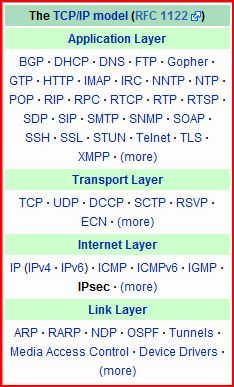
\includegraphics{imagenes/ipsec/modelo_tcp}
	\caption{En este esquema se puede ver claramente el puesto en la pila que opera IPSec.}
	\label{fig:ipsec_modelo_tcp}
	\end{center}
\end{figure}

Los protocolos que emplea IPSec comunmente son \gls{AH} y \gls{ESP}, que en conjunto sirven para asegurar autenticaci�n, integridad, protecci�n contra repetici�n y confidencialidad de la comunicaci�n. Las funciones espec�ficas para cada caracter�stica son las siguientes:

\begin{itemize}
	\item \textbf{Autenticaci�n}. Verifica la identidad del remitente de un paquete.
	\item \textbf{Protecci�n de la integridad}. Asegura que los datos no se han cambiado en el transcurso de la comunicaci�n.
	\item \textbf{Protecci�n contra la repetici�n}. Evita que un atacante pueda guardar paquetes cifrados y luego repetir los mismos sin ser detectado; obteniendo as�, acceso al tr�fico encriptado.
	\item \textbf{Confidencialidad}. Oculta la informaci�n que se esta transmitiendo con cifrado mediante claves compartidas entre remitente y destinatario.
\end{itemize}

Estas caracter�sticas se pueden obtener combinando ambos protocolos (ESP y/o AH) dependiendo del nivel de seguridad que se requiere para la transferencia de datos. Por ejemplo, si se utiliza solo AH se obtienen las tres primeras caracter�sticas pero no ofrece confidencialidad. En cambio ESP puede proveer de todas las caracter�sticas.

Otro protocolo que puede emplear IPSec para el transporte de informaci�n es \gls{IPCOMP}, que permite comprimir los datos que se van a transferir para aprovechar el ancho de banda de la conexi�n. Vemos entonces que se pueden definir diferentes modos para transmitir informaci�n utilizando uno o varios de los protocolos mencionados, cada uno con sus ventajas y desventajas:

\begin{itemize}
	\item Solo AH: Autenticaci�n avanzada, integridad y antirrepetici�n.
	\item Solo ESP: Autenticaci�n (opcional), integridad, antirrepetici�n y cifrado.
	\item ESP y AH: Autenticaci�n avanzada, integridad, antirrepetici�n y cifrado.
	\item ESP e IPCOMP: Autenticaci�n, integridad, antirrepetici�n, cifrado y compresi�n.
	\item AH, ESP e IPCOMP: Autenticaci�n avanzada, integridad, antirrepetici�n, cifrado y compresi�n.
\end{itemize}

Tal como se puede presentir, cuanto m�s tecnolog�as se utilizan, se obtiene una mejora de la seguridad en el tr�fico de informaci�n, pero esto lleva a una alta utilizaci�n de procesamiento para las tareas de cifrado y compresi�n principalmente. Por esta raz�n no siempre es conveniente utilizar todas las opciones juntas, sino las que se adec�an a nuestras necesidades.

\subsection{Componentes de IPSec}

Como se ha mencionado anteriormente, IPSec esta basado en varios protocolos. Estos se pueden dividir en dos grupos seg�n su funci�n: los relacionados con la \emph{gesti�n de claves} y los relacionados con la \emph{manipulaci�n de los datos}. La parte de gesti�n de claves esta comprendida por IKE que esta basado en los protocolos siguientes:

\begin{itemize}
	\item ISAKMP
	\item Oakley Key Determination Protocol
\end{itemize}

En la manipulaci�n de datos se encuentran los protocolos que permiten compresi�n, cifrado, autenticaci�n y manipulaci�n de paquetes, que ya se han listado anteriormente (y aqu� nuevamente):

\begin{itemize}
	\item \gls{AH}
	\item \gls{ESP}
	\item \gls{IPCOMP}
\end{itemize}

Los protocolos de gesti�n de claves son los que realizan la negociaci�n entre las partes y almacenan las claves. Adem�s ayudan a establecer las SA de IPSec.

Por otro lado, los protocolos de manipulaci�n de paquetes utilizan las SA para agregar caracter�sticas de seguridad a los paquetes.

\subsection{Modos de transferencia}

IPSec puede utilizar dos modos de transferencia, por lo que puede crear paquetes en dos formatos soportados: transporte y t�nel. De esta manera se puede proteger el datagrama IP completo o s�lo los protocolos de capas superiores.

En modo t�nel el datagrama IP se encapsula completamente dentro de un nuevo datagrama IP que emplea el protocolo IPsec. En modo transporte IPsec s�lo maneja la carga del datagrama IP, insert�ndose la cabecera IPsec entre la cabecera IP y la cabecera del protocolo de capa superior. La figura \ref{fig:ipsec_modos} muestra el diagrama de los diferentes modos.

\begin{figure}[htb]
	\begin{center}
	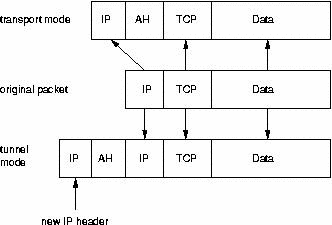
\includegraphics{imagenes/ipsec/tunnel_transport}
	\caption{Comparaci�n de los modos transporte y t�nel junto al paquete original.}
	\label{fig:ipsec_modos}
	\end{center}
\end{figure}

En otras palabras, en el modo \emph{transporte}, IPSec protege los paquetes, encriptando el payload del datagrama IP agregando cabeceras IPSec y los tipos de protecci�n solicitados, entre la informaci�n �til, y la cabecera IP original.

En el modo t�nel, IPSec trata al paquete entero como un bloque de datos, en el que a�ade una nueva cabecera y protege los datos haciendo que formen parte de la informaci�n �til cifrada del paquete nuevo.

En la pr�ctica se utiliza generalmente el modo transporte para las conexiones de host a host, mientras que si se tratan de puertas de enlaces (conexi�n red a red) es conveniente utilizar el modo t�nel.

\subsection{Protocolos de gesti�n e intercambio de claves}

Cuando se utilizan bases de datos de asociaciones de seguridad y de normativas de seguridad, se puede pretender configurarlas tanto manual como autom�ticamente. El modo autom�tico es el m�s utilizado y se lo lleva a cabo con protocolos de gesti�n e intercambio de claves para IPSec.

El protocolo IKE resuelve el problema m�s importante del establecimiento de comunicaciones seguras que es la autenticaci�n de los participantes y el intercambio de claves sim�tricas. Para lograr este cometido crea las \gls{SA} y rellena la \gls{SAD}. Adem�s este protocolo combina elementos, definiciones y funcionalidades de otros protocolos como \gls{ISAKMP}, \gls{SKEME} y \gls{Oakley} para intercambiar y gestionar claves y SA.

\subsubsection{IKE}

El protocolo IKE permite negociar SA autom�ticamente y suele implementarse a trav�s de servidores en espacio de usuario, y no en el sistema operativo. Este funciona sobre UDP y emplea el puerto 500 para su comunicaci�n.

IKE ha sido desarrollado para ofrecer protecci�n ante atacantes que pretendan repetir, eliminar o cambiar mensajes. Adem�s soporta \gls{PFS}. Sin esta caracter�stica, si una clave esta comprometida, las otras claves y SA pueden resultar afectadas tambi�n, por lo tanto, todos los datos cifrados con esa clave. Por eso es recomendable activar esta opci�n.

El protocolo IKE funciona en dos fases. La Fase I establece una SA de ISAKMP con el prop�sito de crear un canal seguro para proteger las siguientes negociaciones. En esta fase las negociaciones tienen lugar con menos frecuencia (una vez a la hora o quiz�s una vez al d�a) que en la Fase II (una vez cada minuto o cada 1024K de datos cifrados).

En la Fase II, se deben negociar las SA de IPSec utilizadas para proteger el tr�fico IP. Todo los mensajes intercambiados en esta fase est�n protegidos por la Fase I.

\subsubsection{M�todos de autenticaci�n}

La autenticaci�n de los participantes en la Fase I se realiza mediante claves compartidas o firmas digitales.

La autenticaci�n mediante \gls{PSK} utiliza una \emph{clave compartida} que deben tener todas las partes que intervienen en el proceso de autenticaci�n. Este m�todo tiene problemas de seguridad y escalabilidad, ya que el transporte de claves en texto claro a los servidores que estan distanciados f�sicamente, hacen que la seguridad dependa de terceros (correo electr�nico, correo tradicional, mensajer�a, etc.). Si la clave cae en manos inapropiadas, la seguridad del sistema puede estar muy comprometida, por m�s que se utilicen los mejores m�todos de encriptaci�n y cifrado de datos, ya que el atacante simular�a ser un nodo de confianza. Por otro lado, si se disponen de numerosos nodos y se mantiene un plan de cambio de claves de forma regular, distribuir las claves por tantos servidores, tiene un costo agregado en la administraci�n de VPN de gran tama�o.

El uso de \emph{firmas digitales} (RSS o RSA) permite firmar los datos con la clave privada, que luego es verificada mediante la clave p�blica del par. De esta manera se verifica la identidad de quien solicita la conexi�n. Con este m�todo se mejora el problema de la distribuci�n de claves, mediante la utilizaci�n de certificados digitales sabiendo que se puede confiar en un tercero para que asocie la identidad del par con su clave p�blica. Se considera este m�todo mejor que el de intercambio directo de claves p�blicas.

En la Secci�n \ref{sec:ipsec_metodos_de_autenticacion} se detallan estos m�todos y se proporcionan ejemplos concretos.

\subsubsection{Fundamentos de la Fase I}

El protocolo IKE realiza varias operaciones importantes, como la de negociar los par�metros y protocolos criptogr�ficos que se utilizan para la autenticaci�n y cifrado. Adem�s se autentican los equipos mediante los algoritmos negociados. Por �ltimo se establece un secreto compartido basado en la informaci�n intercambiada. De esta manera se consigue un canal seguro al finalizar la Fase I. Los modos posibles en esta fase son:

\begin{itemize}
	\item Modo principal.
	\item Modo agresivo.
	\item Modo base.
\end{itemize}

En el \index{Modo principal} se intercambian seis datagramas UDP, y si los host A y B son los que dicen ser, el primer mensaje hace una propuesta y ofrece una lista de protocolos alternativos para que B elija. En el segundo mensaje, B devuelve los protocolos que quiere utilizar junto con otra informaci�n.

En los siguientes mensajes, los hosts intercambian material clave y establecen las claves compartidas, y por �ltimo se autentican mutuamente utilizando el m�todo de autenticaci�n seleccionado en los primeros mensajes.

En el \index{Modo agresivo} se transmiten tres datagramas UDP, por lo que hacen falta menos paquetes para establecer una SA de ISAKMP en la Fase I que en el Modo principal. Entre las ventajas de este modo se encuentran:

\begin{itemize}
	\item Disminuci�n del n�mero de mensajes.
	\item Posibilidad de asociar identidad (no solo direcci�n IP) con una clave precompartida espec�fica o con una normativa de seguridad.
\end{itemize}

El inconveniente de este modo es que realiza c�lculos que consumen recursos del sistema inmediatamente, en respuesta al primer mensaje. Esto significa que un atacante puede enviar una cantidad considerable de propuestas con direcciones IP falsas, lo que podr�a afectar al rendimiento del sistema y conducir a una denegaci�n de servicio. Adem�s cabe se�alar que el grupo de trabajo de IPSec esta considerando eliminar este modo.

Por �ltimo, el \index{Modo base} fue desarrollado para sacar partido a las ventajas del modo agresivo y subsanar sus desventajas. En este modo se envian cuatro datagramas UDP. Adem�s, este modo propone el establecimiento de claves computacionalmente intensivas hasta que se recibe una respuesta de la parte iniciadora para confirmar su existencia.

Sin embargo, el modo base no trata todos los problemas del modo agresivo, por ejemplo, a menos que se utilice cifrado de clave p�blica, la identidad de las partes comunicantes no esta protegida. Esto es as�, porque las claves compartidas se calculan despu�s de que los hosts hayan intercambiado y verificado su informaci�n de identidad.

\subsubsection{Fundamentos de la Fase II}

Luego de haber finalizado las negociaciones en la Fase I, los hosts deben compartir una SA de ISAKMP nueva, para proteger las subsecuentes negociacioes de la Fase II.

El protocolo de negociaci�n de esta fase se denomina \index{Modo r�pido} (QM), que consta de tres mensajes y permite negociar una o m�s SA de IPSec. Cualquier host puede iniciar las negociaciones, pero despu�s todos los involucrados compartir�n las SA de IPSec negociada y las almacenar�n en sus respectivas \gls{SAD}.

En el modo r�pido, ambas partes tienen que negociar una combinaci�n de uno o m�s protocolos, que son enviados como propuestas (al igual que la Fase I), por cada SA de IPSec. Por ejemplo se pueden usar estas combinaciones:

\begin{itemize}
	\item ESP-3DES-MD5
	\item ESP-3DES-SHA-PFS
	\item AH-3DES-MD5-PFS
	\item AH-3DES-SHA-PFS
\end{itemize}

Adem�s, con cada propuesta se env�a la siguiente informaci�n adicional:

\begin{itemize}
	\item Tiempo de vida de la SA de IPSec propuesta.
	\item Grupo DH.
	\item Indicador de modo transporte o t�nel.
	\item Informaci�n de claves.
\end{itemize}

De esta manera queda establecido el intercambio de claves una vez concluida la Fase II. Lo que sigue es la descripci�n de los protocolos de intercambio de claves.

\subsection{Funcionamiento de IPSec}

El procesamiento de paquetes entrantes y salientes en IPSec pueden variar poco y son casi sim�tricos. Por ejemplo, el procesamiento para un paquete IP saliente se describe de la siguiente manera:

\begin{enumerate}
	\item Para saber qu� hacer con el paquete saliente, se comprueba su \gls{SPD} definida por el administrador del sistema.
	\item IPSec agrega la regla establecida en el punto anterior (AH, ESP o IPCOMP\footnote{Estos protocolos se describen con m�s detalles en las siguientes secciones.}).
	\item Ahora el m�dulo IPSec determina qu� par�metros utilizar para proteger el paquete, definidos en las \gls{SA} que se�ala a una entrada concordante de la SPD.
\end{enumerate}

El procesamiento del tr�fico de paquetes entrantes se realiza de la siguiente manera:

\begin{enumerate}
	\item Se determina la SA (asociaci�n de seguridad) en la base de datos SA del host destino.
	\item Se obtiene el \gls{SPI}, direcci�n IP del destino y protocolo de manipulaci�n de datos IPSec (AH o ESP).
	\item Se realiza la autenticaci�n y descifrado correspondientes.
	\item Luego se obtiene la SPD con la informaci�n necesaria para realizar la operaci�n adecuada con el paquete.
\end{enumerate}

Una de las razones por las que no se obtiene primero la SPD es porque el paquete IP puede tener una cabecera cifrada, y que esta contenga informaci�n como n�mero de puerto, el cual resulte necesario para pasar las reglas SPD.

\section{M�todos de Autenticaci�n}
\label{sec:ipsec_metodos_de_autenticacion}

Antes de iniciar una transferencia de datos entre dos hosts en una red, se requiere de un paso previo que se llama \emph{autenticaci�n}. El host solicitado por un determinado servicio, pide al solicitante, que se identifique, que demuestre que est� autorizado para establecer dicha transferencia.

IPSec provee autenticaci�n mutua, es decir, que no es solo el host solicitante el que se identifica, sino tambi�n el solicitado. Esto esto ayuda a incrementar el nivel de seguridad de nuestras VPNs.

El proceso de identificaci�n es lo que se denomina \emph{autenticaci�n}, y existen diferentes m�todos para hacerlo. En esta secci�n se explicar� en que consisten algunos de ellos, y se analizar�n las ventajas y desventajas de los mismos.

\subsection{Pre-Shared Key (PSK)}
\label{subsec:ipsec_psk}

El m�todo de autenticaci�n mediante \texttt{pre-shared key} (clave compartida previamente, en castellano), es el m�s simple de todos. Consiste en una clave (o llave) secreta conocida �nicamente por los hosts que desean establecer la conexi�n VPN. La clave consta de una consecuci�n de caracteres, como por ejemplo ``estaeslaclavesecreta''.

Cuando dos hosts concuerdan autenticar utilizando este m�todo, transmiten al otro la clave para comprobar que sea la misma en ambos. Para hacer esto de forma segura, se utiliza \textendash en general\textendash el protocolo Diffie-Hellman \footnote{El protocolo Diffie-Hellman permite el intercambio secreto de claves entre dos partes que no han tenido contacto previo, utilizando un canal inseguro, y de manera an�nima (no autenticada).} de \cite{dh-wiki}.

La seguridad de la autenticaci�n mediante PSK, radica en el compartimiento seguro de las claves. Por ejemplo, en la casa central de una empresa se instala un servidor VPN que utiliza IPSec y utiliza PSK como m�todo de autenticaci�n. El encargado de la instalaci�n tambi�n tiene a cargo la configuraci�n de los extremos opuestos del servidor, que se encuentran en las sucursales de dicha empresa. Al momento de configurar el ISAKMP (manejador de claves) de la casa central, ha realizado una PSK que tiene que llevar a las sucursales de manera segura; de modo tal que ning�n intruso pueda obtenerlas, y establecer una VPN con la casa central.

El modo m�s seguro para transportarlas, es que este empleado se traslade f�sicamente hasta las sucursales y las configure �l mismo. Cuando las distancias son muy grandes, esto se hace imposible, por lo que hay que volver a confiar en la tecnolog�a. Utilizar una conexi�n segura (encriptada) puede ser una opci�n; por ejemplo puede configurar las sucursales a trav�s de una sesi�n \gls{SSH}, enviarlas al administrador remoto v�a ftps, https, entre otros protocolos seguros.

De esta manera surge una desventaja, que es si alguien llegara a conocer la PSK, los datos \textendash e incluso la integridad de la empresa \textendash corre peligro; por lo que es conveniente que no se la conf�e a cualquier persona, ni que la contrase�a sea de f�cil deducci�n.

\subsection{Certificados Digitales X.509}
\label{subsec:ipsec_certificados_x509}

Con el objeto de comprender los certificados \texttt{X.509}, previamente se ver�n algunos conceptos necesarios para incrementar la seguridad de la VPN.

\subsubsection{Certificados Digitales}

Un \emph{Certificado Digital} es un documento digital mediante el cual un tercero confiable (una autoridad de certificaci�n) garantiza la vinculaci�n entre la identidad de un sujeto o entidad y su clave p�blica.

Existen varios formatos para certificados digitales, pero los m�s com�nmente empleados se rigen por el est�ndar UIT-T X.509. El certificado contiene usualmente el nombre de la entidad certificada, n�mero de serie, fecha de expiraci�n, una copia de la clave p�blica del titular del certificado (utilizada para la verificaci�n de su firma digital) y la firma digital de la autoridad emisora del certificado de forma que el receptor pueda verificar que esta �ltima ha establecido realmente la asociaci�n.

Cualquier persona o instituci�n puede generar un certificado digital, pero si �ste no es reconocido por quienes interact�en con el propietario del certificado, el valor del mismo es pr�cticamente nulo. Para que los certificados emitidos por una entidad sean fiables los emisores deben acreditarse. Ver m�s en \cite{cert-wiki}.

\subsubsection{Autoridad de Certificaci�n}

Una Autoridad de certificaci�n o certificadora (de \cite{ca-wiki}) es una entidad de confianza, responsable de emitir y revocar los certificados digitales, para lo cual se emplea la criptograf�a de clave p�blica.

Para este caso no se requiere de los servicios de una CA externa, se puede firmar por uno mismo los certificados, ya que no se necesita reconocimiento p�blico para este trabajo; e incluso a la hora de implementar una VPN en una empresa, se puede tener su propia autoridad de certificaci�n.

\subsubsection{El est�ndar X.509}

X.509 \textendash en su versi�n 3 \textendash es un formato est�ndar, internacionalmente aceptado, para certificados digitales. Dichos certificados pueden contener informaci�n espec�fica de la organizaci�n a la cual pertenece, que puede ser utilizada para una mejor identificaci�n de la organizaci�n en las operaciones.

La estructura general interna de un certificado X.509 puede verse en la configuraci�n \ref{config:estandar_x509}.

\begin{configuracion_small}
\begin{listing}[style=configuracion_small]
    * Certificado
          o Versi�n
          o N�mero de serie
          o ID del algoritmo
          o Emisor
          o Validez
                + No antes de (fecha)
                + No despu�s de (fecha)
          o Sujeto
          o Informaci�n de clave p�blica del sujeto
                + Algoritmo de clave p�blica
                + Clave p�blica del sujeto
          o Identificador �nico de emisor (opcional)
          o Identificador �nico de sujeto (opcional)
          o Extensiones (optional)
                + ... 
    * Algoritmo usado para firmar el certificado
    * Firma digital del certificado
\end{listing}
\caption{Estructura de un certificado X.509}
\label{config:estandar_x509}
\end{configuracion_small}

El primer campo \textendash luego de la validez \textendash es el \emph{subject} (sujeto), que contiene los datos que identifican al sujeto titular. Estos datos est�n expresados en notaci�n DN (Distinguished Name), donde un DN se compone a su vez de diversos campos, siendo los m�s frecuentes los siguientes; CN (Common Name), OU (Organizational Unit), O (Organization) y C (Country). Un ejemplo para identificar un usuario mediante el DN, es el siguiente:

\begin{itemize}
	\item CN=nicolasformoso.com.ar
	\item O=Proyecto Final
	\item OU=VPN
	\item C=AR
\end{itemize}

Adem�s del nombre del sujeto titular (subject), el certificado tambi�n contiene datos asociados al propio certificado digital, como la versi�n del certificado, su identificador (serialNumber), la CA firmante (issuer), el tiempo de validez (validity), etc.

La versi�n X.509.v3 tambi�n permite utilizar campos opcionales (nombres alternativos, usos permitidos para la clave, ubicaci�n de la CRL y de la CA, etc.).

Luego el certificado contiene la clave p�blica, que consta de dos campos, el que muestra el algoritmo utilizado para crear la clave (ej. RSA), y la propia clave p�blica.

Por �ltimo, la CA ha a�adido la secuencia de campos que identifican la firma de los campos previos. Esta secuencia contiene tres atributos, el algoritmo de firma utilizado, el hash de la firma, y la propia firma digital como se puede ver en \cite{x509-wiki}.

\section{Descripci�n General de la VPN}
\label{sec:ipsec_implementacion}

Nuevamente, como en \emph{VPN usando PPP sobre SSH} (Cap�tulo \ref{chap:vpn_pppsobressh}), la topolog�a seleccionada para la VPN que implementaremos es \emph{Red a Red}.

La diferencia fundamental con la implementaci�n anterior, es que aqu�, el Servidor VPN comparte el mismo hardware que el Firewall, es decir, se encuentran en el mismo equipo; esto refleja una ventaja, dado que pueden crearse reglas para el tr�fico VPN con las mismas herramientas que para el resto del tr�fico de la red; aunque tambi�n se tienen algunas desventajas desventajas (Secci�n \ref{sec:interaccion_con_el_firewall}).

La topolog�a red a red, permite que las redes involucradas en la conexi�n, tengan la impresi�n de que se encuentran unidas solamente por un router; pero en realidad pueden estar separadas por grandes distancias. Las dos redes conectadas a trav�s de Internet y la conexi�n virtual privada establecida entre ellas, se pueden ver en la Figura \ref{fig:vpn_en_fw}.

\begin{figure}[htbp]
\centering
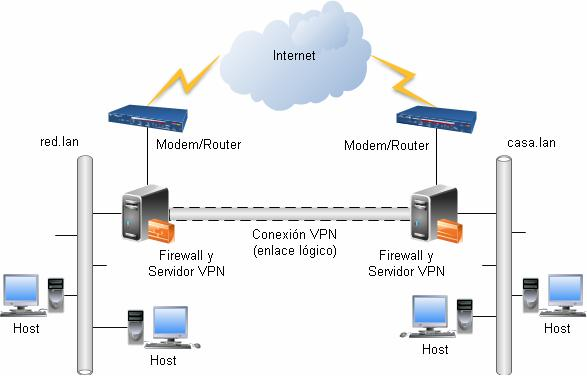
\includegraphics{imagenes/ipsec/vpn_en_fw}
\caption{El servidor VPN en el mismo equipo que el Firewall}
\label{fig:vpn_en_fw}
\end{figure}

El Servidor VPN se ha implementado en el Firewall. Dicho equipo funciona tambi�n como \emph{default gateway} (en castellano, puerta de enlace predeterminada), que es la �nica puerta de entrada/salida de datos a Internet. Esto ayuda a que la auditor�a de seguridad sea sencilla, ya que la misma se reduce a un solo punto de conexi�n.

El sistema operativo de dicho servidor es OpenBSD, que tiene la cualidad de ser sumamente estable y optimizado en cuestiones de seguridad. V�ase la Secci�n \ref{sec:realizacion_entornos} para m�s detalles de los sistemas utilizados.

Finalmente, el protocolo que utilizar� el Servidor VPN es IPSec, ya descrito anteriormente en este mismo cap�tulo. El intercambio de claves ser� autom�tico, por lo que se requerir� para el mismo, el protocolo IKE, que utiliza ISAKMP/Oakley.

\section{Configuraci�n de los nodos}
\label{sec:ipsec_configuracion}

Gracias a la transparencia de este tipo de VPN, los �nicos nodos que necesitan ser configurados son los que establecen la conexi�n. El resto de los nodos \textendash en ambas redes \textendash solo deben tener configurado como puerta de enlace predeterminada al Servidor VPN; esto es as�, ya que dicho servidor se implementa en el mismo \emph{Default Gateway}.

Como los nodos que establecen la VPN tienen el mismo Sistema Operativo \textendash OpenBSD\textendash y los mismos demonios, las configuraciones son similares. Por lo tanto, todo lo que se encuentra explicado en el resto de esta secci�n, es v�lido para ambos nodos, caso contrario se har�n notar las diferencias.

\subsection{Configuraci�n del kernel}

A diferencia de GNU/Linux, OpenBSD maneja los m�dulos del kernel a trav�s de un comando llamado \emph{sysctl}, que permite agregar, modificar y eliminar ciertos par�metros del kernel. En una consola, y con privilegios de superusuario se deben escribir los siguientes comandos para habilitar las opciones de IPSec:

\begin{listing}[style=consola, numbers=none]
$ sudo sysctl net.inet.ip.forwarding=1
$ sudo sysctl net.inet.esp.enable=1
$ sudo sysctl net.inet.ah.enable=1
$ sudo sysctl net.inet.ipcomp.enable=1
\end{listing}

Con las l�neas anteriores el kernel habilita los par�metros especificados, pero si el servidor se apagara por alguna raz�n, habr�a que escribirlas de nuevo. Para evitar esta incomodidad, se las deben especificar en un archivo que las cargar� autom�ticamente durante el arranque. Este es \texttt{/etc/sysctl.conf}, que debe contener las l�neas que aparecen en la Configuraci�n \ref{config:ipsec_sysctl.conf}.

\begin{configuracion}
\begin{listing}[style=configuracion]
net.inet.ip.forwarding=1
net.inet.esp.enable=1
net.inet.ah.enable=1
net.inet.ipcomp.enable=1
\end{listing}
\caption{L�neas necesarias para habilitar el soporte a IPSec.}
\label{config:ipsec_sysctl.conf}
\end{configuracion}

En general, \texttt{/etc/sysctl.conf} ya posee las l�neas 1, 2, 3 y 4 de \ref{config:ipsec_sysctl.conf} (y otras m�s) pero se encuentran comentadas, por lo que habr� que quitar el caracter numeral (\#). El siguiente listado detalla cada l�nea del archivo en cuesti�n:

\begin{enumerate}
	\item \emph{net.inet.ip.forwarding=1}: Como se esta trabajando en una puerta de enlace, esta l�nea esta habilitada. La misma permite que los hosts internos de la red puedan acceder a Internet.
	\item \emph{net.inet.esp.enable=1}: Habilita en el kernel el protocolo ESP de IPSec.
	\item \emph{net.inet.ah.enable=1}: Habilita en el kernel el protocolo AH de IPSec.
	\item \emph{net.inet.ipcomp.enable=1}: Habilita en el kernel el protocolo de compresi�n IPComp, de IPSec.
\end{enumerate}

\subsection{La interface \texttt{enc0}}

Para poder inspeccionar el tr�fico VPN que pasa por nuestro Servidor, se requiere levantar una interfaz llamada \texttt{enc}X, donde X se reemplaza por un n�mero entero. Para levantar la interfaz se ejecuta \emph{ifconfig enc0 up}; pero para que se levante cada vez que se encienda el equipo, se edita y guarda el archivo \texttt{/etc/hostname.enc0}, conteniendo en su interior �nicamente el comando \emph{up}.

La funcionalidad de esta interfaz, viene dada por el hecho de que permite leer los datos antes de ser encriptados, de los paquetes IPSec que se env�an; as� como permite leer los datos de los paquetes IPSec que llegan, luego de ser desencriptados.

\subsection{Directivas de Firewall}
\label{sec:isakmpd_fw}

Cada una de las redes est� protegida por el firewall propio de OpenBSD. Por lo tanto, es necesario habilitar los puertos y permitir el tr�fico de los protocolos utilizados por IPSec, de lo contrario el \emph{Packet Filter} no lo dejar� salir, y descartar� los paquetes. Para comprender mejor el funcionamiento v�ase la Secci�n \ref{sec:ReglasFiltradoOpenBSD}.

Luego se crea un \emph{anchor}, que ser� el que contenga todas las reglas necesarias para establecer VPN. La ventaja de los anchors es que se pueden recargar las reglas contenidas en ellos, sin tener que recargar las reglas principales de PF, ni la de los otros \emph{anchors}.

Para crear un anchor llamado \texttt{vpn\_isakmpd}, simplemente se agrega al archivo \texttt{/etc/pf.conf}, la l�nea:

\begin{verbatim}
anchor vpn_isakmpd
\end{verbatim}

Luego se deben recargar las reglas del PF con el comando \texttt{pfctl -f /etc/pf.conf}. Luego, para ver si el anchor se ha creado satisfactoriamente, se ejecuta \texttt{pfctl -s rules}; esto devuelve todas las reglas cargadas en el firewall, y los anchors si es que los hay.

La siguiente salida en pantalla es un ejemplo del uso de este comando:

\begin{listing}[style=consola, numbers=none]
# pfctl -s rules
scrub in all fragment reassemble
block return all
pass quick on xl0 all flags S/SA keep state
pass quick on lo0 all flags S/SA keep state
pass quick on ppp0 all flags S/SA keep state
anchor "vpn_isakmpd" all
pass in on tun0 inet proto tcp from any to (tun0) port = ssh flags S/SA keep state
pass in on tun0 inet proto tcp from any to (tun0) port = www flags S/SA keep state
pass in on tun0 inet proto tcp from any to (tun0) port = auth flags S/SA keep state
pass in on xl0 inet from 192.168.1.0/24 to any flags S/SA keep state
pass out on xl0 inet from any to 192.168.1.0/24 flags S/SA keep state
pass out on tun0 proto tcp all flags S/SA modulate state
pass out on tun0 proto udp all keep state
pass out on tun0 proto icmp all keep state
#
\end{listing}

Dicho sea de paso, esta es la salida original del comando, de uno de los servidores durante las pruebas. La regla necesaria es \texttt{anchor ``vpn\_isakmpd all''}; esto quiere decir, que el firewall tambi�n leer� todas las reglas que se encuentren es el \emph{anchor}.

Naturalmente, en el \emph{anchor} reci�n creado, no hay reglas definidas. Por esto se crea un archivo nuevo que contiene las reglas necesarias para cargar en el \emph{anchor}; el archivo es: \texttt{/etc/pf.conf.isakmpd}, cuyo contenido se puede ver en la Configuraci�n \ref{config:pfconf_isakmpd}, que esta ubicado en una de las puertas de enlace (m�s espec�ficamente, en \texttt{nicolasformoso.com.ar}).

\begin{configuracion}
\begin{listing}[style=configuracion]
# Interfaces
ext_if="tun0"

# Variables
GUS_DN = "gustavocortez.com.ar"
LOCAL_DN = "nicolasformoso.com.ar"
GUS_NET = "192.168.0.0/24"
LOCAL_NET = "192.168.1.0/24"

## Permitiendo la entrada/salida del tr�fico encriptado,
# solo de la direcci�n que deseamos
pass in proto esp from $GUS_DN to $LOCAL_DN
pass out proto esp from $LOCAL_DN to $GUS_DN
pass in proto ah from $GUS_DN to $LOCAL_DN
pass out proto ah from $LOCAL_DN to $GUS_DN

# Necesitamos permitir el tr�fico "ipencap" en la interfaz enc0
pass in on enc0 proto ipencap from $GUS_DN to $LOCAL_DN

## Permitimos el tr�fico de paquetes entre las subredes locales,
# por la interfaz "enc0"
pass in on enc0 from $GUS_NET to $LOCAL_NET
pass out on enc0 from $LOCAL_NET to $GUS_NET

## Permitimos el tr�fico por el puerto 500 (isakmpd), pero solo
# con un destino especificado ($GUS_DN).
pass in on $ext_if proto udp from $GUS_DN port = 500 to $LOCAL_DN port = 500
pass out on $ext_if proto udp from $LOCAL_DN port = 500 to $GUS_DN port = 500
#$
\end{listing}
\caption{Archivo /etc/pf.conf.isakmpd}
\label{config:pfconf_isakmpd}
\end{configuracion}

B�sicamente lo que se hace, con estas reglas de firewall, es permitir el flujo de paquetes entre las puertas de enlace de las respectivas redes. Al momento de cargarse estas l�neas en el firewall, se resuelven los nombres de dominios y se los reemplaza por la direcci�n IP correspondiente; por lo que si en alg�n momento el ISP cambia la IP asignada anteriormente, es necesario volver a recargar las reglas. Por el contrario, en una empresa que posee direcciones IP p�blicas est�ticas (o fijas), no tienen el mismo problema.

Se utiliza la interfaz \texttt{enc0} para transmitir el tr�fico encapsulado, por lo que se permite el tr�fico a trav�s de ella, desde y hacia el par remoto. Tambi�n se da paso al flujo de paquetes encriptados con IPSec, con ESP y/o AH.

En la siguiente salida en pantalla de la consola se puede observar la ejecuci�n de los comandos para cargar las reglas de \emph{anchor} y para visualizarlas:

\begin{listing}[style=consola, numbers=none]
$ sudo pfctl -a vpn_isakmpd -f /etc/pf.conf.isakmpd
$ sudo pfctl -a vpn_isakmpd -s rules
pass in inet proto esp from 190.137.64.31 to 190.137.67.68 keep state
pass in inet proto ah from 190.137.64.31 to 190.137.67.68 keep state
pass in on enc0 inet proto ipencap from 190.137.64.31 to 190.137.67.68 keep state
pass in on tun0 inet proto udp from 190.137.64.31 port = isakmp to 190.137.67.68 port = isakmp keep state
pass in on enc0 inet from 192.168.0.0/24 to 192.168.1.0/24 flags S/SA keep state
pass out inet proto esp from 190.137.67.68 to 190.137.64.31 keep state
pass out inet proto ah from 190.137.67.68 to 190.137.64.31 keep state
pass out on tun0 inet proto udp from 190.137.67.68 port = isakmp to 190.137.64.31 port = isakmp keep state
pass out on enc0 inet from 192.168.1.0/24 to 192.168.0.0/24 flags S/SA keep state
$
$
\end{listing}

\subsection{Configuraci�n de \texttt{isakmpd}}

El intercambio de claves y la negociaci�n de otros par�metros necesarios para la VPN, se hace en el establecimiento de la misma. Estas gestiones pueden realizarse de forma manual, o autom�tica. En este caso se ha optado por el modo autom�tico, debido a que, la configuraci�n es m�s sencilla y resuelve problemas del intercambio manual de claves, como los ``ataques por repetici�n de paquetes''.

Toda la configuraci�n de este demonio se guarda por defecto en un archivo llamado \texttt{isakmpd.conf}, en el directorio \texttt{/etc/isakmpd}. Adem�s de dicha configuraci�n, existen otros archivos que tambi�n se tienen que analizar y modificar.

\subsubsection{An�lisis de \texttt{isakmpd.conf}}

En el archivo de Configuraci�n \ref{config:isakmpd.conf.psk} se puede ver un ejemplo del contenido del archivo.

Este archivo se divide en secciones, cuyos nombres se encuentran encerrados entre corchetes. Por ejemplo, [General] es la primera secci�n; en ella se definen par�metros globales para todas las conexiones que se puedan definir a continuaci�n. La opci�n \emph{Listen-on=}, permite especificar una lista separadas por comas de las direcciones IP locales y/o interfaces de red, a trav�s de las cuales se establecer�n las VPN.

\begin{configuracion_small}
\begin{listing}[style=configuracion_small]
[General]
Listen-On=              tun0

[Phase 1]
190.225.230.254=        peer-gustavo

[Phase 2]
Connections=            VPN-GUSTAVO

[peer-gustavo]		# <ISAKMP-Peer>
Phase=                  1
Address=    	        190.225.230.254
Configuration=          Default-main-mode
Authentication=         clavesupersecreta

[VPN-GUSTAVO]		# <IPSec-Connection> 
Phase=                  2
ISAKMP-peer=            peer-gustavo
Configuration=          Default-quick-mode
Local-ID=               nicolas-internal-network
Remote-ID=              gustavo-internal-network

[gustavo-internal-network]	# <IPSec-ID>
ID-type=                IPV4_ADDR_SUBNET
Network=		192.168.0.0                
Netmask=                255.255.255.0

[nicolas-internal-network] 	# <IPSec-ID>
ID-type=                IPV4_ADDR_SUBNET
Network=		192.168.1.0                
Netmask=                255.255.255.0

[Default-main-mode]
EXCHANGE_TYPE=          ID_PROT
Transforms=             3DES-SHA,BLF-SHA

[Default-quick-mode]
EXCHANGE_TYPE=          QUICK_MODE
Suites=                 QM-ESP-3DES-SHA-SUITE
\end{listing}
\caption{Archivo \texttt{isakmpd.conf} (con autenticaci�n mediante PSK)}
\label{config:isakmpd.conf.psk}
\end{configuracion_small}

Las secciones \emph{[Phase 1]} y \emph{[Phase 2]} se utilizan durante el establecimiento de la conexi�n en las respectivas fases. En la primera se define el par�metro \texttt{190.225.230.254=}, que es una direcci�n IP p�blica con la cual se va a conectar; a la derecha del s�mbolo igual, se define el nombre de la secci�n que tiene los par�metros para lograr establecer la conexi�n con el equipo remoto. En la segunda secci�n, el par�metro \texttt{Connections=}, es el que define una lista de posibles secciones a utilizar para establecer las SA de IPSec.

La secci�n \emph{[peer-gustavo]} \textendash relacionada en [Phase 1] con una direcci�n IP \textendash, define los par�metros que se utilizar�n para la fase 1 para establecer la conexi�n con dicho host. Lo par�metros que merecen ser destacados son \texttt{Configuration=} que contiene el nombre de la secci�n donde se definen el modo, que puede ser Principal (ID\_PROT) o agresivo (AGRESSIVE), y los algoritmos de encriptaci�n y Hash que se utilizar�n (en este caso, 3DES y SHA respectivamente). El nombre de esta secci�n es \emph{Default-main-mode}.

El siguiente par�metro a ser destacado es \texttt{Authentication=}; este se utiliza solo cuando el m�todo de autenticaci�n es mediante clave \gls{PSK}, y lo que se especifica al lado es dicha clave. Este par�metro debe ser el mismo en los dos nodos que desean establecer la conexi�n.

La secci�n \emph{[VPN-GUSTAVO]} \textendash especificada en [Phase 2] \textendash, contiene los par�metros para la creaci�n de las SA; en el que se tiene \texttt{ISAKMP-peer=}, donde se especifica la secci�n que contiene los par�metros para la fase 1 de la conexi�n, luego \texttt{Configuration=}, que contiene la secci�n donde encuentran los par�metros para establecer la fase 2, en el modo (QUICK\_MODE), y por �ltimo las \texttt{Suites=}, que son una lista de conjuntos de protocolos utilizados para la protecci�n del tr�fico IP (en este caso, se utilizan \texttt{ESP+3DES+SHA}).

En las secciones \texttt{Local-ID=} y \texttt{Remote-ID=} se definen los nombres de las secciones que contienen las definiciones de las redes local y remota respectivamente.

\subsubsection{Configuraci�n de Certificados Digitales X.509}

En el ejemplo del archivo \texttt{/etc/isakmpd/isakmpd.conf} dado anteriormente, el modo de autenticaci�n utilizado es \gls{PSK}.

Ahora se va a configurar un certificado digital X.509 para la autenticaci�n, a fin de tener mayor control de quienes se conectan a la VPN.

Los certificados digitales, para que funcionen, deben ser firmados por una entidad llamada \emph{Autoridad de Certificaci�n}, que es un tercero que da garant�a de que el certificado es de la persona que lo posee, y es v�lido. Para evitar la incomodidad y la demora de estas terceras partes, se crear� una autoridad de certificaci�n propia, que consiste �nicamente en crear una clave privada con la cual se firmar�n los certificados que necesarios \footnote{La CA, no necesariamente debe ser uno de los equipos involucrados en la conexi�n, sino que puede ser cualquier otro con las herramientas para hacerlo.}.

En la siguiente salida por pantalla de la terminal, se puede ver la l�nea necesaria para hacer este trabajo:

\begin{listing}[style=consola, numbers=none]
HOST_CA# openssl req -x509 -days 365 -newkey rsa:1024 -keyout /etc/ssl/private/ca.key \
> -out /etc/ssl/ca.crt
Generating a 1024 bit RSA private key
........................................++++++
......++++++
writing new private key to '/etc/ssl/private/ca.key'
Enter PEM pass phrase: <passphrase>
Verifying - Enter PEM pass phrase: <passphrase>
-----
You are about to be asked to enter information that will be incorporated
into your certificate request.
What you are about to enter is what is called a Distinguished Name or a DN.
There are quite a few fields but you can leave some blank
For some fields there will be a default value,
If you enter '.', the field will be left blank.
-----
Country Name (2 letter code) []: AR
State or Province Name (full name) []: TUC
Locality Name (eg, city) []: SMT
Organization Name (eg, company) []: Proyecto Final
Organizational Unit Name (eg, section) []: CA_TEST
Common Name (eg, fully qualified host name) []: nicolasformoso.com.ar
Email Address []: ca@nicolasformoso.com.ar
HOST_CA#
\end{listing}

El siguiente paso, es la creaci�n de las solicitudes de firma de certificados (los CSR, \emph{Certificate Signing Request}):

\begin{listing}[style=consola, numbers=none]
HOST_VPN1# openssl req -new -key /etc/isakmpd/private/local.key \
>  -out /etc/isakmpd/private/gustavocortez.com.ar.csr
You are about to be asked to enter information that will be incorporated
into your certificate request.
What you are about to enter is what is called a Distinguished Name or a DN.
There are quite a few fields but you can leave some blank
For some fields there will be a default value,
If you enter '.', the field will be left blank.
-----
Country Name (2 letter code) []: AR
State or Province Name (full name) []: TUC
Locality Name (eg, city) []: SMT
Organization Name (eg, company) []: Proyecto Final
Organizational Unit Name (eg, section) []: VPN_IPSec
Common Name (eg, fully qualified host name) []: gustavocortez.com.ar
Email Address []: vpn@gustavocortez.com.ar

Please enter the following 'extra' attributes
to be sent with your certificate request
A challenge password []: <enter>
An optional company name []: <enter>
HOST_VPN1#
\end{listing}

El paso anterior debe realizarse en los dos hosts que pretendan conectarse en la VPN. Este devuelve el CSR para el respectivo host en el archivo \texttt{private/gustavocortez.com.ar.csr}. Luego, las CSR deben ser enviadas a la CA, para ser firmadas por la misma.

La autoridad de certificaci�n, firmar� los certificados X.509 de la siguiente forma:

\begin{listing}[style=consola, numbers=none]
HOST_CA# env CERTFQDN=gustavocortez.com.ar openssl x509 -req -days 365 -in gustavocortez.com.ar.csr -out \
>  gustavocortez.com.ar.crt -CA /etc/ssl/ca.crt -CAkey /etc/ssl/private/ca.key \
>  -CAcreateserial -extfile /etc/ssl/x509v3.cnf -extensions x509v3_FQDN
Signature ok
subject=/C=AR/ST=TUC/L=SMT/O=Proyecto Final/OU=VPN_IPSec/CN=gustavocortez.com.ar/emailAddress=vpn@gustavocortez.com.ar
Getting CA Private Key
Enter pass phrase for /etc/ssl/private/ca.key: <passphrase>
HOST_CA#
\end{listing}

Esto generar� el certificado X.509 firmado, a partir de la solicitud CSR. Dichos certificados deben ser llevados hacia el respectivo host, y deben ser ubicados en el directorio \texttt{/etc/isakmpd/cert}; la ruta al certificado ser�a: \texttt{/etc/isakmpd/cert/gustavocortez.com.ar}. Tambi�n es necesario que la CA otorgue a los hosts el archivo donde se encuentra la firma, es decir, \texttt{/etc/ssl/ca.crt}, que en los hosts debe guardarse en \texttt{/etc/isakmpd/ca}.

Ya est�n dispuestos los certificados en cada host, ahora se debe modificar el archivo \texttt{isakmpd.conf}, para que funcionen. En la Configuraci�n \ref{config:isakmpd.conf.x509} se muestra un ejemplo de dicho archivo para que funcione con certificados X.509.

Se muestran �nicamente las secciones que requieren modificaci�n o se agregan, todas las dem�s quedan como estaban en el caso anterior.

\begin{configuracion_small}
\begin{listing}[style=configuracion_small]
[peer-gustavo]		# <ISAKMP-Peer>
Phase=                  1
Address=    	        190.137.64.31
Configuration=          Default-main-mode
ID=			nicolas-phase1-id

[nicolas-phase1-id]	# <phase1-ID>
ID-type=	FQDN
Name= 		nicolasformoso.com.ar

[Default-main-mode]
EXCHANGE_TYPE=          ID_PROT
Transforms=             3DES-SHA-RSA_SIG,BLF-SHA

[Default-quick-mode]
EXCHANGE_TYPE=          QUICK_MODE
Suites=                 QM-ESP-DES-MD5-AH-MD5-SUITE

[QM-ESP-DES-MD5-AH-MD5-SUITE]
Protocols=              QM-ESP-DES-MD5,QM-AH-MD5

[X509-certificates]
CA-directory=           /etc/isakmpd/ca/
Cert-directory=         /etc/isakmpd/certs/
Private-key=            /etc/isakmpd/private/local.key
\end{listing}
\caption{Secciones del archivo /etc/isakmpd/isakmpd.conf (para autenticaci�n con X.509)}
\label{config:isakmpd.conf.x509}
\end{configuracion_small}

Las �nicas modificaciones necesarias para que funcionen estos certificados, son las que se ven en las secciones \emph{[peer-gustavo]} y \emph{[Default-main-mode]}. En la primera se agrega el par�metro \texttt{ID=}, que define una secci�n de la que se obtiene el \emph{FQDN} local. Este sirve para encontrar el respectivo certificado; en la segunda se cambia 3DES-SHA por 3DES-SHA-RSA\_SIG, en el que el primero es para autenticaci�n mediante PSK y el segundo especifica que se debe buscar un certificado (RSA Signature).

La secci�n \emph{[X509-certificates]} define los directorios donde se ubicar�n las claves y los certificados, si se utilizan los que se definen por defecto, no hace falta especificarla.

Una diferencia entre los dos archivos \texttt{isakmpd.conf} \textendash que no tiene que ver con el modo de autenticaci�n \textendash, es la que hay en la secci�n \emph{[Default-quick-mode]}, se cambi� el modo de protecci�n de tr�fico IPSec de QM-ESP-3DES-SHA-SUITE a QM-ESP-DES-MD5-AH-MD5-SUITE. Con esta nueva suite de protocolos, no solo se agrega la protecci�n que ofrece ESP, sino tambi�n la de AH.

\subsubsection{El archivo \texttt{isakmpd.policy}}

Este archivo es mucho m�s corto que el anterior, pero tambi�n es necesario, por que ayuda a definir la pol�tica para la autenticaci�n, el m�todo, y otras condiciones para agregar seguridad a la VPN con IPSec.

\begin{configuracion_small}
\begin{listing}[style=configuracion_small]
Keynote-version: 2
Authorizer: "POLICY"
Licensees: "DN:/C=AR/ST=TUC/L=SMT/O=Proyecto Final/CN=nicolasformoso.com.ar"
Conditions: app_domain == "IPsec policy" &&
            esp_present == "yes" &&
            esp_enc_alg != "null" -> "true";
\end{listing}
\caption{Archivo \texttt{isakmpd.policy} (para autenticaci�n con X.509)}
\label{config:isakmpd.policy.x509}
\end{configuracion_small}

Un ejemplo de este archivo ser�a como en la Configuraci�n \ref{config:isakmpd.policy.x509}. A continuaci�n se detallan los par�metros:

\emph{Authorizer:}, siempre llevar� el par�metro ``POLICY'', que indica que no hay delegaci�n de autenticaci�n.

\emph{Conditions:} permite agregar condiciones tanto para los protocolos utilizados en la encriptaci�n, hashing, como para las direcciones de los nodos remotos. En el manual se muestra una lista interminable de par�metros que se pueden especificar aqu�.

\emph{Lecensees:} es el que se usar� para indicar c�mo ser� la autenticaci�n. Si esta ausente, esta se har� mediante PSK (especificada en el archivo \texttt{isakmpd.conf}); si est� presente, se puede indicar una PSK, una CA para certificados X.509, o ambas cosas. Por ejemplo, para indicar una PSK, esta l�nea deber�a ser de la siguiente forma:

\begin{verbatim}
Licensees: "passphrase:clavesupersecreta"
\end{verbatim}

Pero si se quieren utilizar los certificados creados anteriormente, es necesario agregar la identificaci�n de la CA, para admitir los certificados firmados por la misma. Esta identificaci�n se obtiene de la siguiente forma:

\begin{listing}[style=consola, numbers=none]
$ cd /etc/isakmpd
$ openssl x509 -in ca/ca.crt -noout -subject
Subject: /C=ar/ST=tuc/L=smt/O=Proyecto Final/CN=nicolasformoso.com.ar
\end{listing}

Por lo que en el archivo \texttt{isakmpd.policy}, se debe agregar la l�nea:

\begin{verbatim}
Licensees: "DN:/C=AR/ST=TUC/L=SMT/O=Proyecto Final/CN=nicolasformoso.com.ar"
\end{verbatim}

Donde DN significa \emph{Distinguished Name}, y es sucedido por la identificaci�n de la CA.

\subsection{Iniciaci�n de la conexi�n}

Para activar las conexiones, lo �nico necesario es hacer correr el demonio; con permisos de superusuario se escribe en una consola simplemente el comando \texttt{isakmpd}. El demonio se ejecutar� independiente de una terminal, si el otro extremo est� activo, se establecer� autom�ticamente la conexi�n, sino se esperar� a que se solicite el establecimiento de la misma.

Para ver las rutas creadas por IPSec, en la consola se ejecuta el siguiente comando:

\begin{listing}[style=consola, numbers=none]
$ netstat -rn -f encap
Routing tables

Encap:
Source             Port  Destination        Port  Proto SA(Address/Proto/Type/Direction)
192.168.1/24       0     192.168.0/24       0     0     190.30.88.184/esp/use/in
192.168.0/24       0     192.168.1/24       0     0     190.30.88.184/esp/require/out
$
\end{listing}

La salida del comando \texttt{netstat} son las rutas creadas entre las redes que establecen la conexi�n, a trav�s de la interfaz \texttt{enc0}. Para poder usarlas, hay que crear (en ambas redes) una ruta de la familia \emph{inet}; con esto se define la interfaz de entrada/salida de los paquetes encapsulados, que en este caso, ser� la interfaz de red local. La Figura \ref{fig:ruteo_isakmpd} refleja esta situaci�n.

\begin{figure}[htbp]
\centering
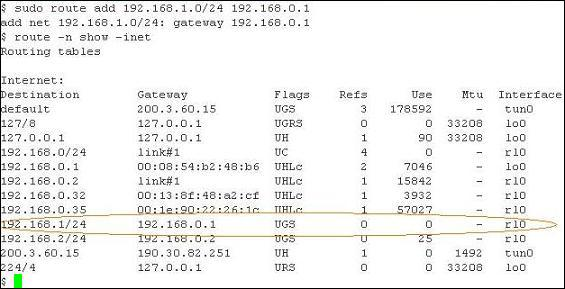
\includegraphics{imagenes/ipsec/ruteo.jpg}
\caption{Configuraci�n de ruteo en nodo isakmpd}
\label{fig:ruteo_isakmpd}
\end{figure}

Cuando se establece la conexi�n con IPSec se crean asociaciones de seguridad (SA) y pol�ticas de seguridad. Para ver las bases de datos correspondientes (SAD y SPD) se utiliza el comando \texttt{ipsecctl}, que tambi�n se utiliza cuando las SA son creadas manualmente.

El comando siguiente devuelve el contenido de la SAD y de la SPD (llamada aqu� FLOWS):

\begin{listing}[style=consola, numbers=none]
$ sudo ipsecctl -s all
FLOWS:
flow esp in from 192.168.1.0/24 to 192.168.0.0/24 peer 190.30.88.184 srcid 190.30.82.251/32 dstid 190.30.88.184/32 type use
flow esp out from 192.168.0.0/24 to 192.168.1.0/24 peer 190.30.88.184 srcid 190.30.82.251/32 dstid 190.30.88.184/32 type require

SAD:
esp tunnel from 190.30.82.251 to 190.30.88.184 spi 0xa2aa4aaa auth hmac-sha1 enc 3des-cbc
esp tunnel from 190.30.88.184 to 190.30.82.251 spi 0xfcd76754 auth hmac-sha1 enc 3des-cbc
$
\end{listing}


\subsubsection{Verificaci�n de la conexi�n}

Por �ltimo, para ver si hay contacto entre los hosts internos de las redes, se pueden realizar unas simples pruebas. En el host \texttt{192.168.1.2} se escribe:

\begin{listing}[style=consola, numbers=none]
# ping -c 2 192.168.0.32
PING 192.168.0.32 (192.168.0.32): 56 data bytes
64 bytes from 192.168.0.32: icmp_seq=0 ttl=127 time=37.797 ms
64 bytes from 192.168.0.32: icmp_seq=1 ttl=127 time=33.252 ms
--- 192.168.0.32 ping statistics ---
2 packets transmitted, 2 packets received, 0.0% packet loss
round-trip min/avg/max/std-dev = 33.252/35.524/37.797/2.280 ms
# ssh 192.168.0.32
ssh: connect to host 192.168.0.32 port 22: Connection refused
#
\end{listing}

Con el comando \texttt{ping} se comprueba si hay respuesta desde la direcci�n \texttt{192.168.0.32}; por lo que se puede ver en la salida anterior, es que s� hay respuesta. Seguidamente se puede intentar establecer una conexi�n SSH con dicho host (cuyo puerto 22 est� cerrado a prop�sito).

Al mismo tiempo de realizadas estas pruebas, en el servidor VPN del lado del host testeado, se estaba ejecutando un sniffer de paquetes (tcpdump) sobre la interfaz \texttt{enc0}; la salida que se obtuvo es la siguiente:

\begin{listing}[style=consola, numbers=none]
$ sudo tcpdump -i enc0
tcpdump: listening on enc0, link-type ENC
11:39:18.882757 (authentic,confidential): SPI 0xcfc4ee73: 192.168.1.2 > 192.168.0.32: icmp: echo request (encap)
11:39:18.883959 (authentic,confidential): SPI 0xb11a0f91: 192.168.0.32 > 192.168.1.2: icmp: echo reply (encap)
11:39:19.885315 (authentic,confidential): SPI 0xcfc4ee73: 192.168.1.2 > 192.168.0.32: icmp: echo request (encap)
11:39:19.886169 (authentic,confidential): SPI 0xb11a0f91: 192.168.0.32 > 192.168.1.2: icmp: echo reply (encap)
11:39:38.183945 (authentic,confidential): SPI 0xcfc4ee73: 192.168.1.2.33209 > 192.168.0.32.ssh: S 3134895536:3134895536(0) win 16384 <mss 1460,nop,nop,sackOK,nop,wscale 0,nop,nop,timestamp 3588245553 0> (DF) (encap)
11:39:38.185066 (authentic,confidential): SPI 0xb11a0f91: 192.168.0.32.ssh > 192.168.1.2.33209: R 0:0(0) ack 3134895537 win 0 (encap)
^C
6 packets received by filter
0 packets dropped by kernel
$
\end{listing}

Se pueden observar los paquetes ICMP hacia y desde la direcci�n \texttt{192.168.0.32}. Luego se ve el intento de conexi�n SSH. M�s pruebas se pueden ver en la Secci�n \ref{sec:ipsec_pruebas_mediciones}.

Al final de cada l�nea en la salida del sniffer (que detalla un paquete) dice \emph{(encap)}, lo que sifnifica que el tr�fico est� encapsulado con IPSec.

\section{Pruebas y mediciones}
\label{sec:ipsec_pruebas_mediciones}

En esta secci�n se van a detallar las aplicaciones utilizadas para comprobar que la comunicaci�n se ha establecido correctamente y que la informaci�n llega a todos los puntos de la red interna. Tambi�n se va mostrar el flujo de informaci�n que atraviesa la VPN de un extremo a otro.

Por �ltimo se realizan mediciones en la velocidad de transferencia de archivos y en en las conexi�n a escritorios remoto. Adem�s se van a realizar comprobaciones de la vulnerabilidad del sistema con un software especializado.

\subsection{Revisi�n del tr�fico}

Una manera de ver si llegan los paquetes a destino o simplemente si atraviesan el firewall, es utilizar un filtro de paquetes. En OpenBSD se tiene \gls{tcpdump} en modo texto y en Windows (o cualquier otro sistema operativo) se puede utilizar el software libre \gls{Wireshark} en modo gr�fico.

La siguiente salida por pantalla muestra el tr�fico de paquetes que llegan de un host remoto, que han pasando por el proceso de encapsulado, autenticaci�n y cifrado de IPSec:

\begin{listing}[style=consola, numbers=none]
$ sudo tcpdump -i enc0
tcpdump: listening on enc0, link-type ENC
11:39:18.882757 (authentic,confidential): SPI 0xcfc4ee73: 192.168.1.2 > 192.168.0.32: icmp: echo request (encap)
11:39:18.883959 (authentic,confidential): SPI 0xb11a0f91: 192.168.0.32 > 192.168.1.2: icmp: echo reply (encap)
11:39:19.885315 (authentic,confidential): SPI 0xcfc4ee73: 192.168.1.2 > 192.168.0.32: icmp: echo request (encap)
11:39:19.886169 (authentic,confidential): SPI 0xb11a0f91: 192.168.0.32 > 192.168.1.2: icmp: echo reply (encap)
11:39:38.183945 (authentic,confidential): SPI 0xcfc4ee73: 192.168.1.2.33209 > 192.168.0.32.ssh: S 3134895536:3134895536(0) win 16384 <mss 1460,nop,nop,sackOK,nop,wscale 0,nop,nop,timestamp 3588245553 0> (DF) (encap)
11:39:38.185066 (authentic,confidential): SPI 0xb11a0f91: 192.168.0.32.ssh > 192.168.1.2.33209: R 0:0(0) ack 3134895537 win 0 (encap)
^C
6 packets received by filter
0 packets dropped by kernel
$
\end{listing}

De esta manera se ha comprobado que por la interfaz \texttt{enc0} viajan los datos encapsulados desde una red a la otra.

\subsection{Comprobaci�n de la ruta de paquetes}

Para comprobar el recorrido de los paquetes transmitidos por la red se ha utilizado \gls{traceroute} en los sistemas BSD y Linux, y \gls{tracert} en Windows. La siguiente salida en pantalla desde un equipo con Windows (cliente DHCP) que se le ha asignado la direcci�n IP 192.168.0.35, efect�a la traza hasta un equipo de otra red, a trav�s de la VPN, cuya direcci�n de destino es 192.168.1.3.

\begin{listing}[style=consola, numbers=none]
C:\\Users\\Gustavo>tracert 192.168.1.3

Traza a la direcci�n PONCHO [192.168.1.3]
sobre un m�ximo de 30 saltos:

  1    <1 ms    <1 ms    <1 ms  192.168.0.1
  2    70 ms    42 ms    39 ms  192.168.1.2
  3    38 ms    39 ms    39 ms  PONCHO [192.168.1.3]

Traza completa.

C:\\Users\\Gustavo>
\end{listing}

Se puede observar del listado anterior que el paquete primero llega a la puerta de enlace predeterminada del sistema local (es decir, 192.168.0.1), y luego el servidor que previamente ha establecido las rutas para interconectar las redes mediante la VPN, reenv�a este paquete a la puerta de enlace remota (del otro extremo de la VPN) de direcci�n IP 192.168.1.2, que a su vez reenv�a el paquete al equipo destino que pertenece a su red. En el siguiente listado se puede ver la operaci�n invertida.

\begin{listing}[style=consola, numbers=none]
C:\\Documents and Settings\\Admin>tracert 192.168.0.32

Traza a 192.168.0.32 sobre caminos de 30 saltos como m�ximo.

  1    <1 ms    <1 ms    <1 ms  192.168.1.2
  2    38 ms   150 ms    77 ms  192.168.0.1
  3   352 ms   194 ms   361 ms  192.168.0.32

Traza completa.

C:\\Documents and Settings\\Admin>
\end{listing}

En esta situaci�n, el equipo con direcci�n IP 192.168.1.3 realiza la traza de paquetes hacia un equipo de otra red, pasando por la VPN, y finalmente llegando a destino (de IP 192.168.0.32).

\subsection{Transferencia de archivos}

La transferencia de archivos se realiza a una velocidad aceptable, pero que depende de la capacidad de subida del enlace. El proveedor actual (ISP) permite una subida de 256 Kbps, por lo que se aproxima a casi 30 Kbytes por segundos te�rico. En la Figura \ref{fig:ipsec_transferencia_archivo} se puede observar que la transferencia ronda los 24 Kbytes por segundo; esto resulta aceptable para las condiciones en que se realiza la transmisi�n, es decir, el retardo de las puertas de enlace, la franja horaria, distancia, entre otras condiciones.

\begin{figure}[htbp]
	\centering
		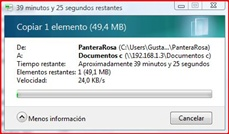
\includegraphics{imagenes/ipsec/ipsec_transferencia_archivo}
		\caption{Captura de pantalla de una transferencia de archivo mediante IPSec.}
	\label{fig:ipsec_transferencia_archivo}
\end{figure}

Adem�s se tiene en cuenta que la transferencia se realiza mediante el protocolo \gls{SMB} que utiliza Windows para la transferencia de archivo mediante el explorador de archivos, y que este no es el m�todo m�s r�pido para transferir archivos. A�n as�, los resultados mediante \gls{FTP} fueron similares.

\subsection{Escritorio remoto}

Tambi�n se ha evaluado el rendimiento mediante conexiones \gls{VNC} al escritorio remoto de un equipo de cada red, separada por la VPN. La Figura \ref{fig:ipsec_vnc} muestra la velocidad de conexi�n entre dos equipos de subred diferente, de ambos extremos de la VPN.

\begin{figure}[htbp]
	\centering
		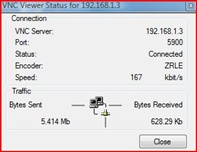
\includegraphics{imagenes/ipsec/ipsec_vnc}
		\caption{Captura de pantalla de una seci�n de VNC.}
	\label{fig:ipsec_vnc}
\end{figure}

Finalmente, se ha comprobado que la conexi�n se manten�a estable, pero el rendimiento del escritorio remoto se hac�a cada vez m�s ``pesado'' a medida que se acercaba a la franja horaria pico en cuanto a cantidad de conexiones al ISP. A pesar de esto, la comunicaci�n en ning�n momento se ha perdido.

\subsection{Buscando vulnerabilidades}

En la comprobaci�n de seguridad de un sistema (en realidad de toda la red), se pueden utilizar varias herramientas que por lo general tienen un costo bastante elevado. Por esta raz�n es que para estas pruebas se ha utilizado un programa gratuito propiedad de \emph{Tenable Network Security} denominado \gls{Nessus}.

Nessus trabaja en modo cliente y servidor, donde el primero genera el informe y muestra al usuario los resultados del escaner, el segundo realiza el monitoreo en el servidor residente.

\begin{figure}[htbp]
	\centering
		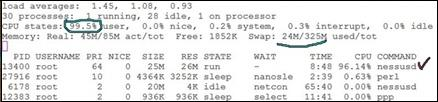
\includegraphics{imagenes/ipsec/ipsec_top_nessus1}
		\caption{Captura de pantalla del programa \texttt{top} en OpenBSD.}
	\label{fig:ipsec_top_nessus}
\end{figure}

En la Figura \ref{fig:ipsec_top_nessus} se puede ver que el consumo de recursos que utiliza el servidor Nessus para comprobar las vulnerabilidades de los sistemas, es excesivamente elevado, llegando a consumir casi el 99 por ciento de microprocesador durante un largo proceso de escaneo. Adem�s utiliza mucha cantidad de memoria, a tal punto que requiere, en la mayor�a de los casos, utilizar la memoria de intercambio \gls{swap}.

\section{Conclusi�n}
\label{sec:ipsec_conclusion}

El uso de IPSec para establecer una VPN presenta un gran desaf�o para los administradores de sistemas. Esto se debe a la dificultad propia de la tecnolog�a que muchas veces pueden llegar a hacer tomar decisiones incorrectas. Como se menciona en \cite{redesprivadasvirtualesconlinux}, seg�n los cript�grafos, la complejidad es un enemigo de la seguridad.

Por esta raz�n, es necesario establecer una buena pol�tica de seguridad previa a la configuraci�n y puesta en funcionamiento de IPSec. Esto implica que si la seguridad del sistema esta comprometida, la implementaci�n de IPSec no va a subsanar el problema. De hecho, las normativas de seguridad son impuesta por los administradores del sistema, IPSec solamente ofrece los mecanismos para asegurarlo.

Nuevamente la utilizaci�n de sistemas complejos como IPSec requieren de mucho estudio y pr�ctica en entornos reales. La gran cantidad de conceptos que maneja, pueden llevar a los administradores a filtrar detalles o a pasar por alto normativas que estan fuera del alcance de IPSec.

Por otro lado, si se realiza una buena combinaci�n de protocolos y m�todos de autentificaci�n cuidadosamente distribuidos, IPSec puede llegar a ser la mejor soluci�n para mantener enlaces seguros entre las partes.

Adem�s se puede decir que IPSec se encuentra dentro de los protocolos y sistemas m�s seguros que puedan utilizarse para establecer una VPN red a red entre dos o m�s enlaces. Pero como se ha mencionado anteriormente, IPSec no protege los gateway ni los ataques de denegaci�n de servicios, por lo que su configuraci�n y puesta en funcionamiento se encuentra estrechamente relacionada con la pol�tica de seguridad y de las directivas de un buen firewall protegiendo el equipo y las redes involucradas.

Finalmente el grupo de desarrollo de IPSec esta considerando disminuir la complejidad del mismo, eliminando algunos componentes tales como el modo transporte, el modo agresivo e incluso el protocolo AH. Esto se realiza con el objetivo de simplificar la tarea de los administradores y para que no sea necesario estudiar todas las RFC para aprender a manejar IPSec.


%% VPN con OpenVPN
%%%%%%%%%%%%%%%%%%%%%%%%%%%%%%%%%%%%%%%%%%%%%%%%%%%%%%%%
%   |-------------------------|                        %
%   |REDES PRIVADAS VIRTUALES |                        %
%   |                         |                        %
%   | Proyecto de graduaci�n  |                        %
%   |_________________________|                        %
%                                                      %
%   Autores                                            %
%   -------                                            %
%                                                      %
% * Formoso Requena, Nicol�s Federico (CX02-0239-8)    %
%     nicolasformoso@gmail.com                         %
% * Cortez, Gustavo Maximiliano (CX01-0801-9)          %
%     cmgustavo83@gmail.com                            %
%                                                      %
%   Tutores                                            %
%   -------                                            %
%                                                      %
% * Ing. Gustavo Vanetta - vanettag@gmail.com          %
% * Lic. Miguel Bazzano - miguelbazzano@gmail.com      %
%                                                      %
%%%%%%%%%%%%%%%%%%%%%%%%%%%%%%%%%%%%%%%%%%%%%%%%%%%%%%%%

% ********* VPN con OpenVPN ********** %

\chapter{VPN con OpenVPN}
\label{chap:vpn_con_openvpn}

OpenVPN es una implementaci�n de una VPN de c�digo abierto, utilizado para crear t�neles encriptados entre hosts. Se pueden establecer enlaces directos entre los equipos involucrados, a pesar que est�n detr�s de un firewall, utilizando NAT. Fue inicialmente escrito por James Yonan y publicado bajo licencia GPL.

En este cap�tulo se introducir� a la tecnolog�a de OpenVPN; se describir�n sus fundamentos y caracter�sticas importantes, que hacen de esta, una buena alternativa de \gls{IPSec}, para usuarios m�viles. Tambi�n se realizar�n pruebas de comprobaci�n de funcionamiento y de transferencia de archivos.

\section{Introducci�n}
\label{sec:openvpn_introduccion}

OpenVPN permite autenticar los pares utilizando claves pre compartidas, certificados o nombre de usuario y contrase�a. Un servidor que acepta m�ltiples clientes, puede autenticar a cada cliente utilizando firmas y certificados autorizados.

OpenVPN incorpora OpenSSL como librer�a de encriptaci�n. No es compatible con \gls{IPSec} y con ninguna otra soluci�n VPN expuesta en este trabajo. Los paquetes de instalaci�n constan de archivos binarios para la conexi�n entre el cliente y el servidor.

Seg�n \cite{wikibooks_openvpn} esta soluci�n se ha ideado para simplificar la configuraci�n de VPN dejando atr�s los tiempos de soluciones complejas como IPSec.

\subsection{Encriptaci�n y autenticaci�n}

OpenVPN utiliza OpenSSL para proveer de encriptaci�n a los datos. Este paquete realiza todo el trabajo de encriptaci�n y autenticaci�n.

OpenVPN puede utilizar las caracter�sticas de autenticaci�n de \gls{HMAC} para agregar otra capa de seguridad a la conexi�n. Tambi�n se puede utilizar aceleraci�n por hardware para mejorar la performance de la encriptaci�n.

Existen tres m�todos de autenticaci�n para conectar entre las partes, mediante el uso de claves pre compartidas, con certificados o con nombre de usuario y contrase�a.

\subsection{Funcionamiento}
OpenVPN puede trabajar sobre UDP (lo hace por defecto) o TCP. Multiplexando las comunicaciones sobre un simple puerto TCP o UDP. Puede funcionar a trav�s de servidores proxy y NAT atravesando firewalls.

El m�todo de conexi�n se realiza via las interfaces TUN/TAP, donde la primera esta basada en t�nel IP de capa 3 y la segunda en Ethernet TAP de capa 2. Tambi�n se pueden utilizar librer�as de compresi�n de datos como \gls{LZO}.

El puerto que utiliza OpenVPN de forma oficial es el 1194. Adem�s el uso de protocolos de red comunes (TCP/UDP) hacen una buena alternativa a IPSec en situaciones donde el ISP bloquee protocolos VPN espec�ficos con la finalidad de suscribir a los clientes a soluciones costosas para beneficio propio.

\subsection{Comparaci�n con IPSec}

El Cuadro \ref{tab:comparacion_openvpn_ipsec} muestra un res�men comparativo de OpenVPN frente a IPSec.

\begin{table}[htb]
\begin{center}
	\begin{tabular}{l l}
		\hline
		\textbf{IPSec}                      & \textbf{OpenVPN}                            \\
		\hline
		Estandar VPN                        & A�n desconocido y no compatible con IPSec   \\
		Hardware variado                    & Solo en computadoras                        \\
		Tecnolog�a conocida y probada       & Tecnolog�a nueva y en crecimiento           \\
		Modificaci�n compleja de la pila IP & Tecnolog�a sencilla                         \\
		Requiere modificaciones al kernel   & Interfaces de red y paquetes estandar       \\
		Permisos de administrador           & Se ejecuta en espacio de usuario            \\
		Problemas con direcciones din�micas & Trabaja con servidor DNS din�micos          \\
		Varios puertos y protocolos de uso  & Utiliza un solo puerto del firewall         \\
		\hline
	\end{tabular}
\end{center}
\caption{Comparaci�n entre IPSec y OpenVPN}
\label{tab:comparacion_openvpn_ipsec}
\end{table}

El Cuadro \ref{tab:comparacion_openvpn_ipsec} es una comparativa entre OpenVPN e IPSec. La mayor ventaja del primero respecto al segundo, es la facilidad de uso y puesta en marcha.

\subsection{Seguridad en OpenVPN}

Para encriptar datos se usan contrase�as o claves de encriptaci�n. OpenVPN tiene dos modos considerados seguros, uno basado en claves est�ticas pre compartidas y otro en SSL/TLS usando certificados y claves RSA.

Cuando ambos lados usan la misma clave para encriptar y desencriptar los datos, se esta usando el mecanismo conocido como ``clave sim�trica'' y dicha clave debe ser instalada en todos los equipos que formar�n parte en la conexi�n VPN.

Si bien las claves asim�tricas RSA son la opci�n m�s segura, las claves est�ticas cuentan con la ventaja de ser mucho m�s simples.

\subsubsection{Encriptaci�n sim�trica y claves pre compartidas}

Siempre quien posea la clave puede desencriptar el tr�fico de paquetes, por lo que si esta resulta comprometida, el tr�fico completo de la organizaci�n se ver�a afectado, ya que identificar�a al intruso como un integrante m�s de la VPN.

Es por ello que los mecanismos que utiliza IPSec cambian las claves cada cierto per�odo de tiempo asociando a las mismas un ``tiempo de vida'', como se ha visto en el Cap�tulo \ref{chap:vpn_con_ipsec}.

\subsubsection{Encriptaci�n asim�trica con SSL/TLS}

SSL/TLS usa una de las mejores tecnolog�as de encriptaci�n para asegurar la identidad de los integrantes de la VPN. Cada integrante tiene dos claves, una p�blica y otra privada.

La p�blica es distribuida y usada por cualquiera para encriptar los datos que ser�n enviados a la contraparte quien conoce la clave privada, que es la �nica que sirve para desencriptar los datos. El par de claves p�blica y privada, se generan a partir de algoritmos matem�ticos que aseguran que solo con la clave privada es posible leer los datos originales.

\subsubsection{Seguridad SSL/TLS}

Las bibliotecas SSL/TLS son parte del sofware \emph{OpenSSL}, que viene instalado por defecto en casi todas las distribuciones de Linux y OpenBSD, e implementan mecanismos de encriptaci�n y autenticaci�n basados en certificados. Los certificados generalmente son emitidos por entidades de reconocida confiabilidad aunque tambi�n se pueden emitir unos propios (ver Secci�n \ref{subsec:ipsec_certificados_x509} para m�s detalles) y usarlos en la VPN. Con un certificado firmado, el due�o del mismo es capaz de probar su identidad a todos aquellos que conf�en en la autoridad certificadora que lo ha emitido.

\subsection{Ventajas y desventajas}

OpenVPN provee seguridad, estabilidad y comprobados mecanismos de encriptaci�n sin tener la complejidad de otras soluciones VPN como IPsec, por ejemplo. Adem�s ofrece \emph{ventajas} que van m�s all� que cualquier otra soluci�n como se listan a continuaci�n:

\begin{itemize}
	\item Posibilidad de implementar dos modos b�sicos en capa 2 o capa 3 con lo que se logran t�neles capaces de enviar informaci�n en otros procolos no-IP como IPX o broadcast (NETBIOS).
	\item Protecci�n de los usuarios remotos. Una vez que OpenVPN ha establecido un t�nel el firewall de la organizaci�n proteger� el equipo remoto aun cuando no es un equipo de la red local. 
	\item Las conexiones con OpenVPN pueden ser realizadas a trav�s de casi cualquier firewall. Si se posee acceso a Internet y se puede acceder a sitios HTTPS, entonces un t�nel OpenVPN deber�a funcionar sin ning�n problema.
	\item Soporte para proxy. Funciona a trav�s de proxy y puede ser configurado para ejecutar como un servicio TCP o UDP y adem�s como servidor (simplemente esperando conexiones entrantes) o como cliente (iniciando conexiones).
	\item Solo un puerto en el firewall debe ser abierto para permitir conexiones, dado que desde OpenVPN 2.0 se permiten m�ltiples conexiones en el mismo puerto TCP o UDP.
	\item Las interfaces virtuales (tun0, tun1, etc.) permiten la implementaci�n de reglas de firewall muy espec�ficas.
	\item Todos los conceptos de reglas, restricciones y reenv�o pueden ser utilizados con t�neles OpenVPN.
	\item Alta flexibilidad y posibilidades de extensi�n mediante \emph{scripting}. OpenVPN ofrece numerosos puntos para ejecutar scripts individuales durante su arranque.
	\item Soporte transparente para IPs din�micas. Se elimina la necesidad de usar direcciones IP est�ticas en ambos lados del t�nel.
	\item Ning�n problema con NAT. Tanto los clientes como el servidor pueden estar en la red usando solamente IPs privadas.
	\item Instalaci�n sencilla en cualquier plataforma. Tanto la instalaci�n como su uso son simples.
	\item Dise�o modular. Se basa en un buen dise�o modular con un alto grado de simplicidad tanto en seguridad como en red.
\end{itemize}

Se puede tomar como una \emph{desventaja} que no es IPSec-compatible siendo que justamente IPSec es el est�ndar para soluciones VPN. Adem�s existe a�n poca gente que conoce c�mo usar OpenVPN. No posee interfaz gr�fica. Todav�a no existen soluciones en caja cerrada, solo se pueden establecer conexi�nes entre computadoras, pero ya se est�n desarrollando soluciones de este tipo, que separan las conexiones VPN de los hosts.

\section{Configuraci�n en Linux}
\label{sec:openvpn_configuracion_linux}

A pesar de que existe una versi�n de OpenVPN para sistemas Windows, incluso con una interfaz gr�fica que simplifica un poco las cosas, en esta secci�n se explicar�n los pasos para la configuraci�n bajo Linux, ya que son semejantes en cualquier sistema.

Primero se describir�n los paquetes de software necesarios la instalaci�n de OpenVPN, para la generaci�n de claves  para el servidor y los clientes. Finalmente se detallar�n los archivos de configuraci�n para ambos extremos.

\subsection{Instalaci�n de software}

Para tener todos los componentes necesarios para configurar OpenVPN, se deben instalar los siguientes paquetes de software (algunos sistemas los traen instalados):

\begin{itemize}
	\item OpenSSL.
	\item LZO (opcional si se requiere compresi�n).
	\item OpenVPN.
	\item Controlador tun/tap (ya vienen incluidos en el kernel a partir de la versi�n 2.4.7).
\end{itemize}

\subsection{Creaci�n de certificados y claves RSA}
\label{subsec:openvpn_certificados}

Existen dos formas de conseguir seguridad en una VPN con OpenVPN, uno basado en SSL/TLS mediante certificados y claves RSA y otro en mediante claves est�ticas pre compartidas.

Se utilizar� OpenSSL para contruir los certificados y claves RSA. Adem�s, se crear� un certificado raiz propio, por lo que la \gls{SA} ser� el mismo servidor local. Los pasos para crearlos se resumen en el listado siguiente:

\begin{enumerate}
	\item Crear un certificado CA con el cual se firmar�n y/o revocar�n certificados de clientes.
	\item Crear un certificado y una clave p�blica para los clientes.
	\item Firmar ese certificado usando el certificado CA.
	\item Distribuir la clave y certificados a los clientes.
	\item Configurar los scripts del servidor y de los clientes.
\end{enumerate}

Para empezar, OpenVPN cuenta con varias herramientas y scripts que permiten cumplir con los primeros tres pasos, pero antes se deben crear los directorios y copiar los archivos de ejemplo y scripts.

\begin{listing}[style=consola, numbers=none]
gustavo@wasa:~$ sudo mkdir /etc/openvpn
gustavo@wasa:~$ sudo mkdir /etc/openvpn/keys
gustavo@wasa:~$ sudo cd /etc/openvpn/
gustavo@wasa:/etc/openvpn$ sudo cp /usr/share/doc/openvpn/examples/easy-rsa/2.0/ /etc/openvpn/
\end{listing}

Luego editar el archivo ``vars'' solo cambiando las opciones siguientes que aparecen en la Configuraci�n \ref{config:openvpn_vars}.

\begin{configuracion}
\begin{listing}[style=configuracion]
export KEY_COUNTRY="AR"
export KEY_PROVINCE="TUCUMAN"
export KEY_CITY="SMT"
export KEY_ORG="Proyecto"
export KEY_EMAIL="gustavo@superhijitus.red.lan"
\end{listing}
\caption{Par�metros que deben modificarse en el archivo ``vars''.}
\label{config:openvpn_vars}
\end{configuracion}

Luego se debe obtener permiso de superusuario y ejecutar el script (o establecer los permisos adecuados para que el usuario pueda escribir en todo el directorio). Hacemos lo siguiente:

\begin{listing}[style=consola, numbers=none]
gustavo@wasa:/etc/openvpn$ sudo su
root@wasa:/etc/openvpn# source ./vars
NOTE: If you run ./clean-all, I will be doing a rm -rf on /etc/openvpn/keys
root@wasa:/etc/openvpn# ./clean-all
root@wasa:/etc/openvpn# exit
gustavo@wasa:/etc/openvpn$
\end{listing}

Ahora se intenta crear la clave \emph{Diffie-Hellman} con el script ``build-dh'' lo cual tardar� varios minutos:

\begin{listing}[style=consola, numbers=none]
root@wasa:/etc/openvpn# ./build-dh
Generating DH parameters, 1024 bit long safe prime, generator 2
This is going to take a long time
........................+..................++*++*++*
root@wasa:/etc/openvpn#
\end{listing}

Luego se crea el certificado para la CA:

\begin{listing}[style=consola, numbers=none]
root@wasa:/etc/openvpn# ./build-ca
Generating a 1024 bit RSA private key
............................................................++++++
..........++++++
writing new private key to 'ca.key'
-----
You are about to be asked to enter information that will be incorporated
into your certificate request.
What you are about to enter is what is called a Distinguished Name or a DN.
There are quite a few fields but you can leave some blank
For some fields there will be a default value,
If you enter '.', the field will be left blank.
-----
Country Name (2 letter code) [AR]:
State or Province Name (full name) [TUCUMAN]:
Locality Name (eg, city) [SMT]:
Organization Name (eg, company) [Proyecto]:
Organizational Unit Name (eg, section) []:
Common Name (eg, your name or your server's hostname) [Proyecto CA]:
Email Address [gustavo@superhijitus.red.lan]:
root@wasa:/etc/openvpn#
\end{listing}

De esta manera se han creado los siguientes archivos en el directorio ``keys'':

\begin{itemize}
	\item ca.crt
	\item ca.key
	\item dh1024.pem
\end{itemize}

Para generar el par \emph{Certificado/Clave del servidor}, se utiliza el siguiente comando:

\begin{listing}[style=consola, numbers=none]
root@wasa:/etc/openvpn# ./build-key-server openvpn-server
Generating a 1024 bit RSA private key
....................................++++++
...++++++
writing new private key to 'openvpn-server.key'
-----
You are about to be asked to enter information that will be incorporated
into your certificate request.
What you are about to enter is what is called a Distinguished Name or a DN.
There are quite a few fields but you can leave some blank
For some fields there will be a default value,
If you enter '.', the field will be left blank.
-----
Country Name (2 letter code) [AR]:
State or Province Name (full name) [TUCUMAN]:
Locality Name (eg, city) [SMT]:
Organization Name (eg, company) [Proyecto]:
Organizational Unit Name (eg, section) []:
Common Name (eg, your name or your server's hostname) [openvpn-server]:
Email Address [gustavo@superhijitus.red.lan]:

Please enter the following 'extra' attributes
to be sent with your certificate request
A challenge password []:
An optional company name []:
Using configuration from /etc/openvpn/otro/openssl.cnf
Check that the request matches the signature
Signature ok
The Subject's Distinguished Name is as follows
countryName           :PRINTABLE:'AR'
stateOrProvinceName   :PRINTABLE:'TUCUMAN'
localityName          :PRINTABLE:'SMT'
organizationName      :PRINTABLE:'Proyecto'
commonName            :PRINTABLE:'openvpn-server'
emailAddress          :IA5STRING:'gustavo@superhijitus.red.lan'
Certificate is to be certified until Oct 22 02:34:42 2018 GMT (3650 days)
Sign the certificate? [y/n]:y


1 out of 1 certificate requests certified, commit? [y/n]y
Write out database with 1 new entries
Data Base Updated
root@wasa:/etc/openvpn#
\end{listing}

El par�metro que importa es el Common Name, dado que el mismo ser� utilizado en la configuraci�n de los clientes. El script anterior ha creado los siguientes archivos:

\begin{itemize}
	\item openvpn-server.crt
	\item openvpn-server.csr
	\item openvpn-server.key
\end{itemize}

Ahora se debe crear el par \emph{Certificado/Clave de los clientes}, de la siguiente manera:

\begin{listing}[style=consola, numbers=none]
root@wasa:/etc/openvpn# ./build-key openvpn-client
Generating a 1024 bit RSA private key
.........++++++
...++++++
writing new private key to 'openvpn-client.key'
-----
You are about to be asked to enter information that will be incorporated
into your certificate request.
What you are about to enter is what is called a Distinguished Name or a DN.
There are quite a few fields but you can leave some blank
For some fields there will be a default value,
If you enter '.', the field will be left blank.
-----
Country Name (2 letter code) [AR]:
State or Province Name (full name) [TUCUMAN]:
Locality Name (eg, city) [SMT]:
Organization Name (eg, company) [Proyecto]:
Organizational Unit Name (eg, section) []:
Common Name (eg, your name or your server's hostname) [openvpn-client]:
Email Address [gustavo@superhijitus.red.lan]:

Please enter the following 'extra' attributes
to be sent with your certificate request
A challenge password []:
An optional company name []:
Using configuration from /etc/openvpn/otro/openssl.cnf
Check that the request matches the signature
Signature ok
The Subject's Distinguished Name is as follows
countryName           :PRINTABLE:'AR'
stateOrProvinceName   :PRINTABLE:'TUCUMAN'
localityName          :PRINTABLE:'SMT'
organizationName      :PRINTABLE:'Proyecto'
commonName            :PRINTABLE:'openvpn-client'
emailAddress          :IA5STRING:'gustavo@superhijitus.red.lan'
Certificate is to be certified until Oct 22 03:01:24 2018 GMT (3650 days)
Sign the certificate? [y/n]:y


1 out of 1 certificate requests certified, commit? [y/n]y
Write out database with 1 new entries
Data Base Updated
root@wasa:/etc/openvpn#
\end{listing}

De esta manera se obtienen los siguientes archivos:

\begin{itemize}
	\item openvpn-client.crt
	\item openvpn-client.csr
	\item openvpn-client.key
\end{itemize}

Ahora queda determinar qu� archivos quedan en el servidor y cuales deben ser enviados a los clientes. En la tabla \ref{tab:openvpn_archivos} se muestran los archivos generados y la ubicaci�n de los mismos.

\begin{table}[htb]
\begin{center}
	\begin{tabular}{l l l}
		\hline
		\textbf{Archivo}    & \textbf{Descripci�n}          & \textbf{Ubicaci�n}    \\
		\hline
		dh1024.pem          & Par�metros Diffie Hellman     & Servidor              \\
		ca.crt              & Certificado ra�z CA           & Servidor y Clientes   \\
		ca.key              & Clave ra�z CA                 & Solo equipo que firma \\
		openvpn-server.crt  & Certificado del servidor      & Servidor              \\
		openvpn-server.key  & Clave del servidor            & Servidor              \\
		openvpn-client.crt  & Certificado del cliente       & Cliente               \\
		openvpn-client.key  & Clave del cliente             & Cliente               \\
		\hline
	\end{tabular}
\end{center}
\caption{Archivos generados y ubicaciones para una conexi�n con OpenVPN.}
\label{tab:openvpn_archivos}
\end{table}

\subsection{Configuraci�n del servidor}

Para realizar la configuraci�n del servidor, se debe crear un archivo llamado ``server.conf'' en el mismo directorio que se ha trabajado para generar las claves, cuyo contenido puede ser el de la Configuraci�n \ref{config:openvpn_servidor}.

\begin{configuracion}
\begin{listing}[style=configuracion]
port 1194
proto udp
dev tun
ca keys/ca.crt
cert keys/openvpn-server.crt
key keys/openvpn-server.key
dh keys/dh1024.pem
server 10.8.0.0 255.255.255.0
ifconfig-pool-persist ipp.txt
keepalive 10 120
comp-lzo
persist-key
persist-tun
verb 3
\end{listing}
\caption{Ejemplo de server.conf para OpenVPN.}
\label{config:openvpn_servidor}
\end{configuracion}

\subsection{Configuraci�n del cliente}
\label{subsec:openvpn_configuracion_cliente}

Para la configuraci�n del cliente se utiliza el archivo de configuraci�n ``client.conf'' que se muestra en la Configuraci�n \ref{config:openvpn_cliente}.

\begin{configuracion}
\begin{listing}[style=configuracion]
client
dev tun
proto udp
remote 10.8.0.1 1194
resolv-retry infinite
nobind
persist-key
persist-tun
ca keys/ca.crt
cert keys/openvpn-client.crt
key keys/openvpn-client.key
comp-lzo
verb 3
\end{listing}
\caption{Ejemplo de client.conf para OpenVPN.}
\label{config:openvpn_cliente}
\end{configuracion}

\subsection{Directivas del firewall}

Para dejar pasar el tr�fico de datos de OpenVPN, se debe habilitar el paso por las nuevas interfaces que se crean al iniciar el servidor y recibir una conexi�n de alg�n cliente. En este caso se van a crear interfaces \emph{tunX}, donde X representa el n�mero de la interfaz o nueva conexi�n de un cliente. Los siguientes comandos permiten que iptables deje circular la informaci�n que pase por estas interfaces:

\begin{listing}[style=consola, numbers=none]
root@wasa:/etc/openvpn# iptables -A INPUT -i tun+ -j ACCEPT
root@wasa:/etc/openvpn# iptables -A FORWARD -i tun+ -j ACCEPT
root@wasa:/etc/openvpn# iptables -A OUTPUT -o tun+ -j ACCEPT
root@wasa:/etc/openvpn# iptables -A FORWARD -o tun+ -j ACCEPT
\end{listing}

Solo queda iniciar los servicios correspondientes en el servidor y el cliente, para establecer las conexiones. En el servidor ejecutamos \emph{/etc/init.d/openvpn start}, para levantar el demonio.

Supongamos el caso, que tenemos dos clientes, en el servidor deber�amos ver dos t�neles parecidos a estos, al ejecutar el comando \emph{ifconfig}:

\begin{listing}[style=consola, numbers=none]
tun0      Link encap:UNSPEC  HWaddr 00-00-00-00-00-00-00-00-00-00-00-00-00-00-00-00
          inet addr:10.8.0.1  P-t-P:10.8.0.2  Mask:255.255.255.255
          UP POINTOPOINT RUNNING NOARP MULTICAST  MTU:1500  Metric:1
          RX packets:0 errors:0 dropped:0 overruns:0 frame:0
          TX packets:0 errors:0 dropped:0 overruns:0 carrier:0
          collisions:0 txqueuelen:100
          RX bytes:0 (0.0 B)  TX bytes:0 (0.0 B)

tun1      Link encap:UNSPEC  HWaddr 00-00-00-00-00-00-00-00-00-00-00-00-00-00-00-00
          inet addr:10.8.0.6  P-t-P:10.8.0.5  Mask:255.255.255.255
          UP POINTOPOINT RUNNING NOARP MULTICAST  MTU:1500  Metric:1
          RX packets:0 errors:0 dropped:0 overruns:0 frame:0
          TX packets:0 errors:0 dropped:0 overruns:0 carrier:0
          collisions:0 txqueuelen:100
          RX bytes:0 (0.0 B)  TX bytes:0 (0.0 B)
\end{listing}

\section{Clientes m�viles con Windows}
\label{sec:openvpn_clientes_windows}

En esta secci�n se describen algunos detalles de configuraci�n y ejecuci�n. Adem�s se comprueba la comunicaci�n establecida entre un cliente m�vil (con el sistema operativo Windows) y el servidor OpenVPN con Linux.

El esquema de conexi�n para los clientes m�viles se muestra en la Figura \ref{fig:openvpn_road_warrior}.

\begin{figure}[htb]
	\centering
	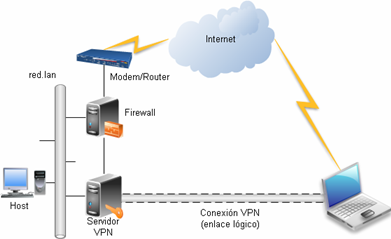
\includegraphics{imagenes/openvpn/road_warrior}
	\caption{Esquema de conexi�n tipo ``Road warrior'' o clientes m�viles.}
	\label{fig:openvpn_road_warrior}
\end{figure}

\subsection{Conexi�n a la red}

Existe una versi�n compilada para Windows de OpenVPN, tanto el servidor como el cliente. Pero adem�s, se cuenta con una versi�n con interfaz gr�fica que provee al usuario de un �cono de conexi�n al servidor en el �rea de notificaci�n, como se muestra en la Figura \ref{fig:openvpn_tray}.

\begin{figure}[htb]
	\centering
	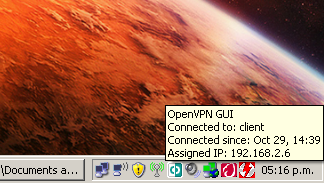
\includegraphics{imagenes/openvpn/tray}
	\caption{En el �rea de notificaci�n se muestra el icono de conexi�n a OpenVPN.}
	\label{fig:openvpn_tray}
\end{figure}

A trav�s de esta herramienta es posible conectar con la red remota simplemente haciendo clic en ``Conectar''. Luego se muestra la direcci�n IP asignada, el nombre de la red a la que se conecta (que puede ser configurada por uno mismo) y la fecha y hora que se ha realizado la conexi�n.

\subsection{Configuraci�n del cliente}

De la misma manera que en la configuraci�n del cliente en la Secci�n \ref{subsec:openvpn_configuracion_cliente}, cada usuario requiere un m�nimo de configuraci�n, que por cierto, se pueden extraer los ejemplos que provee el paquete de instalaci�n.

Los archivos de ejemplo tanto para cliente como para servidor llevan la extensi�n .ovpn y se los obtiene del directorio ``config-examples''. El contenido del archivo de configuraci�n del cliente puede contener el listado de la Configuraci�n \ref{config:openvpn_config_windows}.

\begin{configuracion}
\begin{listing}[style=configuracion]
client
dev tun
proto udp
remote 192.168.0.2 1194
resolv-retry infinite
nobind
persist-key
persist-tun
ca ca.crt
cert openvpn-client1.crt
key openvpn-client1.key
comp-lzo
verb 3
\end{listing}
\caption{Ejemplo de client.ovpn para OpenVPN en Windows.}
\label{config:openvpn_config_windows}
\end{configuracion}

Como se indica en la Configuraci�n \ref{config:openvpn_config_windows}, se utilizan certificados para conectar al servidor, que deben ser generados y distribuidos como en la Secci�n \ref{subsec:openvpn_certificados}.

Por lo tanto, los archivos que deben copiarse al directorio de configuraci�n son los siguientes:

\begin{itemize}
	\item ca.crt
	\item openvpn-client1.key
	\item openvpn-client1.crt
\end{itemize}

Luego, al realizar la conexi�n, el cliente muestra un registro de los pasos que realiza desde el intercambio de claves hasta la asignaci�n de la direcci�n IP (Registro \ref{logs:openvpn_cliente_windows}).

\begin{logs}
  \begin{alltt}
  \scriptsize
  Wed Oct 29 14:39:33 2008 OpenVPN 2.0.9 Win32-MinGW [SSL] [LZO] built on Oct  1 2006
	Wed Oct 29 14:39:33 2008 LZO compression initialized
	Wed Oct 29 14:39:33 2008 Control Channel MTU parms [ L:1542 D:138 EF:38 EB:0 ET:0 EL:0 ]
	Wed Oct 29 14:39:33 2008 Data Channel MTU parms [ L:1542 D:1450 EF:42 EB:135 ET:0 EL:0 AF:3/1 ]
	Wed Oct 29 14:39:33 2008 Local Options hash (VER=V4): '41690919'
	Wed Oct 29 14:39:33 2008 Expected Remote Options hash (VER=V4): '530fdded'
	Wed Oct 29 14:39:33 2008 UDPv4 link local: [undef]
	Wed Oct 29 14:39:33 2008 UDPv4 link remote: 190.30.82.251:1194
	Wed Oct 29 14:39:33 2008 TLS: Initial packet from 190.30.82.251:1194, sid=f0f3ce6e b77f8414
	Wed Oct 29 14:39:33 2008 VERIFY OK: depth=1,
	/C=AR/ST=Tucuman/L=SMT/O=Cissu/CN=Cissu_CA/emailAddress=gustavo@superhijitus.red.lan
	Wed Oct 29 14:39:33 2008 VERIFY OK: depth=0,
	/C=AR/ST=Tucuman/L=SMT/O=Cissu/CN=Cissu_CA/emailAddress=gustavo@superhijitus.red.lan
	Wed Oct 29 14:39:34 2008 Data Channel Encrypt: Cipher 'BF-CBC' initialized with 128 bit key
	Wed Oct 29 14:39:34 2008 Data Channel Encrypt: Using 160 bit message hash 'SHA1' for HMAC authentication
	Wed Oct 29 14:39:34 2008 Data Channel Decrypt: Cipher 'BF-CBC' initialized with 128 bit key
	Wed Oct 29 14:39:34 2008 Data Channel Decrypt: Using 160 bit message hash 'SHA1' for HMAC authentication
	Wed Oct 29 14:39:34 2008 Control Channel: TLSv1, cipher TLSv1/SSLv3 DHE-RSA-AES256-SHA, 1024 bit RSA
	Wed Oct 29 14:39:34 2008 [Cissu_CA] Peer Connection Initiated with 190.30.82.251:1194
	Wed Oct 29 14:39:35 2008 SENT CONTROL [Cissu_CA]: 'PUSH_REQUEST' (status=1)
	Wed Oct 29 14:39:35 2008 PUSH: Received control message: 'PUSH_REPLY,route 192.168.0.0 255.255.255.0,
	route 192.168.2.1,topology net30,ping 10,ping-restart 120,ifconfig 192.168.2.6 192.168.2.5'
	...
	\end{alltt}
  \caption{Estableciendo la conexi�n desde el cliente OpenVPN.}
  \label{logs:openvpn_cliente_windows}
\end{logs}

Aunque el registro \ref{logs:openvpn_cliente_windows} muestra solo una parte de la salida en la interfaz gr�fica del cliente, se puede ver en el listado que se permite compresi�n de paquetes, luego se realiza el intercambio de claves y finalmente se establecen las direcciones IP y rutas correspondientes.

\subsection{Modificaci�n de rutas}

Para poder hacer pruebas de ``ping'' entre el equipo remoto y el servidor OpenVPN junto a la red local, es necesario establecer las rutas correspondientes en el firewall, es decir en el equipo con OpenBSD.

Para esto se ejecuta el siguiente comando:

\begin{listing}[style=consola, numbers=none]
$ sudo route add 192.168.2.0/24 192.168.0.2
$
\end{listing}

De esta manera se agrega una nueva entrada a la tabla de ruteo que se puede ver a continuaci�n:

\begin{listing}[style=consola, numbers=none]
$ route show -inet
Routing tables

Internet:
Destination        Gateway            Flags    Refs      Use    Mtu  Interface
default            200.3.60.15        UGS         2   177818      -   tun0
loopback           localhost          UGRS        0        0  33208   lo0
localhost          localhost          UH          1       90  33208   lo0
192.168.0/24       link#1             UC          4        0      -   rl0
superhijitus       00:08:54:b2:48:b6  UHLc        2     7012      -   lo0
192.168.0.2        link#1             UHLc        1    15842      -   rl0
192.168.0.32       00:13:8f:48:a2:cf  UHLc        1     3684      -   rl0
192.168.0.35       00:1e:90:22:26:1c  UHLc        1    56610      -   rl0
192.168.1/24       superhijitus       UGS         0       22      -   rl0
192.168.2/24       192.168.0.2        UGS         0       25      -   rl0
200.3.60.15        host251.190-30-82. UH          1        0   1492   tun0
BASE-ADDRESS.MCAST localhost          URS         0        0  33208   lo0
$
\end{listing}

En una terminal de Windows tambi�n se puede ver que el cliente m�vil alcanza la red local a la cual se ha conectado mediante el servidor OpenVPN. En la Figura \ref{fig:openvpn_ipconfig_cliente} se puede ver una captura de pantalla que muestra el comando ``ipconfig'' con la direcci�n IP asignada (junto a la direcci�n local), y el comando ``ping'' al firewall con OpenBSD donde se han asignado las rutas.

\begin{figure}[htb]
	\centering
	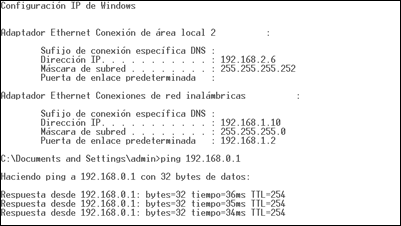
\includegraphics{imagenes/openvpn/ping}
	\caption{Prueba del alcance del equipo remoto a la nueva red.}
	\label{fig:openvpn_ipconfig_cliente}
\end{figure}

Puede verse entonces, que el equipo remoto no solo puede alcanzar al servidor OpenVPN que asigna la direcci�n a la red 192.168.2.0 sino que tambi�n puede acceder a la red 192.168.0.0 mediante un simple ruteo.

Esta normativa de asignar direcciones de red diferentes sirve para distinguir a los usuarios remotos de los usuarios de la red local, pero a�n as� permitiendo a los primeros, el acceso a todo o parte de la red de la empresa.

\subsection{Pruebas de transferencia}

Para las pruebas de transferencia se ha utilizado el protocolo \gls{SMB}, mediante el montaje de una unidad virtual del servidor con el contenido compartido del equipo remoto. Luego se copia un archivo de m�sica al directorio personal del servidor como se muestra en la Figura \ref{fig:openvpn_transferencia}, en el que se muestra la ubicaci�n de origen, destino y velocidad de transferencia.

\begin{figure}[htb]
	\centering
	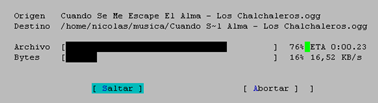
\includegraphics{imagenes/openvpn/samba_transf}
	\caption{Transferencia de archivos entre el equipo remoto y el servidor.}
	\label{fig:openvpn_transferencia}
\end{figure}

El cliente m�vil puede utilizar todos los servicios de la red local como si de un usuario de la misma se tratara.

\section{Conclusi�n}

OpenVPN es un producto de software dise�ado y desarrollado para simplificar los problemas que se tienen con protocolos complejos como IPSec. Esto hace que se convierta en una soluci�n alternativa al est�ndar, y gracias a que es de c�digo abierto, se encuentra siempre en constante actualizaci�n y desarrollo.

Otra ventaja, es que OpenVPN se convirti� en una alternativa a \gls{PPTP}, ya que permite la conexi�n de usuarios m�viles utilizando el software cliente que adem�s esta disponible para cualquier sistema operativo, y salvando los problemas de seguridad de PPTP (Ver m�s detalles en Secci�n \ref{sec:pptp_introduccion}).

Finalmente se puede decir que OpenVPN presenta una muy buena alternativa de f�cil administraci�n y configuraci�n para establecer conexiones seguras. Aunque no supera la seguridad y robustez que tiene IPSec, la simplicidad de uso ha impulsado que este desarrollo de libre distribuci�n vaya adquiriendo cada vez m�s adeptos.


%% Comparativas y costos de implementaci�n
%%%%%%%%%%%%%%%%%%%%%%%%%%%%%%%%%%%%%%%%%%%%%%%%%%%%%%%%
%   |-------------------------|                        %
%   |REDES PRIVADAS VIRTUALES |                        %
%   |                         |                        %
%   | Proyecto de graduaci�n  |                        %
%   |_________________________|                        %
%                                                      %
%   Autores                                            %
%   -------                                            %
%                                                      %
% * Formoso Requena, Nicol�s Federico (CX02-0239-8)    %
%     nicolasformoso@gmail.com                         %
% * Cortez, Gustavo Maximiliano (CX01-0801-9)          %
%     cmgustavo83@gmail.com                            %
%                                                      %
%   Tutores                                            %
%   -------                                            %
%                                                      %
% * Ing. Gustavo Vanetta - vanettag@gmail.com          %
% * Lic. Miguel Bazzano - miguelbazzano@gmail.com      %
%                                                      %
%%%%%%%%%%%%%%%%%%%%%%%%%%%%%%%%%%%%%%%%%%%%%%%%%%%%%%%%

% ********* Alternativas y costos de implementaci�n ********** %

\chapter{Alternativas y costos de implementaci�n}
\label{chap:alternativas_costos_implementacion}

Ning�n paquete de software que se ha visto a lo largo de este informe puede afrontar todos los problemas y requisitos posibles que se pueden encontrar al implementar una red privada virtual. En este cap�tulo se plantean y describen brevemente las soluciones alternativas (o complementarias en algunos casos) a los est�ndares descriptos y probados anteriormente.

Adem�s se plantear�n los criterios que se utilizan al evaluar la mejor soluci�n VPN para una determinada empresa, junto a los costos de instalaci�n y mantenimiento del sistema. Esto puede variar con el pa�s, regi�n, tama�o de la empresa, alcance de la VPN, seguridad requerida, entre muchos otros factores que intervienen en cada caso. Tambi�n se evaluar�n las diferentes soluciones en cuanto a costos y las mejoras que implicar�an su implementaci�n.

\section{Soluciones comerciales}
\label{sec:alternativas_soluciones_comerciales}

Dentro de la amplia gama de posibilidades que existen para implementar seguridad en las redes utilizando VPNs, existen por supuesto, las soluciones comerciales de hardware propietario. 

VPNC~\footnote{M�s informaci�n: http://www.vpnc.org}, es el Consorcio VPN. Un grupo de fabricantes que analiza y certifica los productos VPN comerciales. B�sicamente, VPNC ofrece informes de compatibilidad de los productos de sus miembros. Este consorcio ha sido de gran ayuda para la cooperaci�n entre las empresas, y para que dichos productos sean dise�ados en base a los est�ndares de internet.

En las siguientes secciones se describir�n brevemente los equipos que ofrecen soluciones VPN de las empresas m�s importantes en cuanto a redes y seguridad.

\subsubsection{Cisco ASA 5500 Series SSL/IPsec VPN Edition}

Es un servidor VPN que ofrece acceso a la red corporativa tanto a usuarios m�viles, oficinas remotas, clientes, etc. Se integra en el equipo funcionalidad de firewall, que detecta usuarios no autorizados y seguridad a la red.

Existen varios modelos dentro de la serie; diferenci�ndose en el n�mero de conexiones simult�neas admitidas, que van desde 10 hasta 10.000. Por supuesto que el costo de los equipos, tambi�n crece con el n�mero de usuarios que admiten al mismo tiempo.

Por ejemplo, la licencia para un equipo que admite veinticinco conexiones VPN (modelo ASA5500-SSL-25), llega a US\$ 2,682.53 (precio de Estados Unidos).

\subsubsection{Cisco VPN 3002 Hardware Client - pasarela VPN}

Es un dispositivo separado del computador, que funciona con todos los sistemas operativos, ya que no interfiere con el procesamiento del ordenador. Se utiliza para comunicar a los clientes VPN con la red corporativa de su empresa. Este equipo est� preparado para conectar desde estaciones de trabajo, hasta servidores, impresoras, etc.

El coste de este producto es de US\$598,00.

\subsubsection{Linksys RV082}

Ruteador con conexi�n a Internet compartida de alta fiabilidad y conmutador de ocho puertos para negocios peque�os; Consta de puertos de Internet duales para el equilibrio de carga y conexiones redundantes. Conecta de forma segura hasta cincuenta usuarios (de QuickVPN) remotos o itinerantes a la red de su oficina mediante una VPN. Soporta tambi�n cinco conexiones PPTP. 

El coste en Argentina de este router es de US\$514,00.

\subsubsection{Router Draytek Vigor 2930}

Un equipo similar al anterior. Posee 4 puertos LAN y 2 WAN para balanceo de carga. Tiene capacidad para soportar hasta cien t�neles VPN; soporta protocolos IPSec/PPTP/L2TP. Posee firewall, entre otras caracter�sticas.

El coste en Argentina de este router es de US\$375,00.

\section{Soluciones alternativas}
\label{sec:alternativas_soluciones_alternativas}

Actualmente existen varias soluciones alternativas a las escritas en este informe y a las soluciones comerciales de grandes empresas. En esta secci�n se har�n menci�n de dichas soluciones que pueden ser gratuitas o de libre distribuci�n, pero no est�ndar en el mundo de las redes privadas virtuales.

En cuanto a las aplicaciones gratuitas que existen para establecer una VPN entre dos puntos, la m�s conocida por los amantes de los juegos en red, es \emph{LogMeIn Hamachi}. Otra soluci�n que se puede encontrar, m�s orientado al acceso a escritorio remoto es \emph{DESKTRA} (Virtual Private Desktop).

Finalmente se pueden rescatar algunos proyectos de c�digo abierto que intentan implementar una red privada virtual minimizando la tarea de configuraci�n y administraci�n, sacrificando importantes caracter�sticas en cuanto a performance y seguridad de una red corporativa.

\subsection{LogMeIn Hamachi}

Hamachi es un servicio de VPN basado en paquetes UDP que se instala cada equipo (funciona en Windows, MacOSX y Linux) y permite la conexi�n r�pida y segura de los mismos de manera que parezcan estar en una misma red.

De las caracter�sticas que tiene, la que m�s se destaca es su facilidad de uso. Nada m�s crear una red e invitar a otros equipos (mediante contrase�a) a unirse, o directamente ingresar en una red previamente creada por alg�n otro usuario. Por su parte, la lista oficial de caracter�sticas son las siguientes:

\begin{itemize}
	\item Permite compartir archivos y carpetas mediante \gls{SMB}.
	\item Funciona sin tener que configurar firewall.
	\item Utiliza cifrado y autenticaci�n.
	\item Gratuito para uso no comercial.
\end{itemize}

\subsubsection{Funcionamiento}

En el momento de instalar el software, se crea una interfaz de red virtual en el sistema, que va a realizar el tunelado de la informaci�n que se env�e por la VPN (o a trav�s del software en este caso).

Cada cliente establece una conexi�n de control con el cluster servidor, en el que realiza una secuencia de identificaci�n de usuario, seguida de un proceso de descubrimiento y sincronizaci�n de estado. El descubrimiento es utilizado para determinar la topolog�a de la conexi�n a Internet del cliente, es decir, si se encuentra tras un firewall o servidor NAT. El paso de sincronizaci�n se realiza para ver los clientes conectados a la misma red.

Cuando se conectan o desconectan clientes, el servidor emite instrucciones a los otros nodos de la red para que inicien o detengan t�neles con el cliente. Cuando se establecen t�neles entre los nodos, Hamachi utiliza una t�cnica de NAT transversal asistido por servidor, similar a ``UDP hole punching'' (perforadora de agujeros UDP).

En algunas configuraciones NAT no esta garantizado el funcionamiento de Hamachi, que seg�n su desarrollador, atraviesa con �xito el 95 por ciento de conexiones P2P.

Hamachi asigna a cada cliente una direcci�n IP de la red 5.0.0.0/8, que al autenticarse por primera vez se le asigna una direcci�n �nica y luego se la asociada con la clave de cifrado p�blica del cliente.

\subsubsection{Utilidad}

Como se ha mencionado anteriormente, Hamachi se utiliza habitualmente para juegos en red y para la administraci�n remota. De esta manera, cada usuario que se conecte mediante el cliente, puede crear una nueva red, para jugar partidas en l�nea con juegos que solamente funcionan en redes LAN. La Figura \ref{fig:alternativas_hamachi_1} muestra la interfaz de usuario para crear una nueva red. La interfaz para conectarse a una red existente es similar.

\begin{figure}[htb]
	\begin{center}
	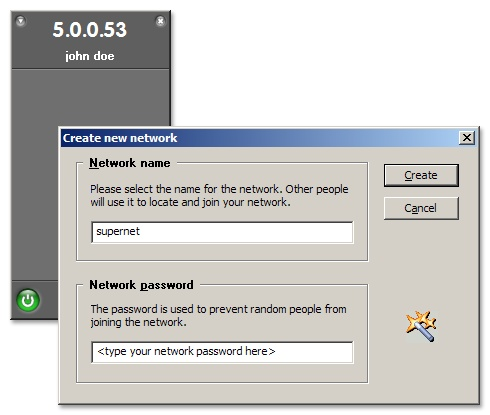
\includegraphics{imagenes/hamachi_1}
	\caption{Interfaz de usuario de Hamachi para crear una nueva red.}
	\label{fig:alternativas_hamachi_1}
	\end{center}
\end{figure}

La utilizaci�n de contrase�a solamente se usa para evitar conexiones no deseadas, de manera que se puede distribuir la contrase�a (como si de una clave p�blica se tratara) entre los usuarios de confianza para que puedan acceder a la red.

\subsection{DESKTRA Virtual Private Desktops}

Este software que se distribuye de forma gratuita para usos no comerciales, permite la conexi�n a escritorios remotos utilizando t�cnicas que se utilizan en las VPN.

Se puede considerar DESKTRA como un software \gls{VNC}, pero difiere en las siguientes caracter�sticas principales (algunas comunes a VNC):

\begin{itemize}
	\item Protecci�n por contrase�a.
	\item Encriptaci�n mediante AES (Advanced Encryption Standard).
	\item No requiere modificaci�n en el firewall ni en el sistema.
\end{itemize}

La desventaja de este sistema es que solamente funciona en equipos con Windows y que adem�s deben instalarse dos paquetes de software, el cliente en un extremo y el servidor en otro. Esto puede resultar poco pr�ctico, ya que si se quiere conectar a un escritorio remoto, la mejor soluci�n est�ndar es utilizar VNC.

Su difusi�n es muy limitada, principalmente por la desventaja descripta anteriormente y adem�s por las mejores alternativas que existen en el mercado.

\subsection{VTun}

VTun o t�nel virtual es una soluci�n VPN escrita por Maxim Krasnyansky, que utiliza interfaces de t�neles en los que los datos se cifran al entrar en el t�nel y se descifran al salir por el t�nel del otro extremo.

Su funcionamiento se basa en encapsular paquetes dentro de paquetes IP y utilizar redes IP para encaminar dichos paquetes encapsulados de una extremo a otro del t�nel. Cada extremo tiene informaci�n sobre el otro, como la direcci�n de red legible y la red que esta detr�s. De esta manera, si un paquete llega con destino a la red que se encuentra del otro lado del t�nel, se lo encamina por la interfaz del t�nel local.

El kernel es el encargado de encapsular y redireccionar el nuevo paquete a la direcci�n conocida del otro extremo del t�nel.

\subsubsection{Funcionamiento}

VTun utiliza el driver TUN/TAP como punto de acceso l�gico al t�nel. De esta manera, los paquetes encaminados al driver creado, en realidad viajan al otro extremo del t�nel. La siguiente salida en pantalla muestra la denominaci�n de la interfaz que crea el sistema para realizar este tipo de conexiones:

\begin{listing}[style=consola, numbers=none]
tun0: flags=8051<UP,POINTOPOINT,RUNNING,MULTICAST> mtu 1492
        groups: tun egress
        inet 190.30.82.251 --> 200.3.60.15 netmask 0xffffffff
\end{listing}

En el ejemplo anterior se puede ver que la interfaz utilizada recibe la direcci�n IP local y del router, que se utiliza al establecer una conexi�n con el proveedor de acceso a Internet. Esto no representa una creaci�n de VTun pero es un ejemplo aproximado.

VTun utiliza un \textsl{daemon} de ejecuci�n denominado \texttt{vtund} que es el responsable de la inicializaci�n y recepci�n de las conexiones de los t�neles, adem�s del mantenimiento de cualquier t�nel establecido. Puede trabajar en modo servidor o cliente, seg�n sea su configuraci�n. Si se lo configura en modo servidor, este espera conexiones entrantes de los clientes y enviar� los par�metros de t�nel configurados de vuelta al cliente. Si en cambio se lo configura en modo cliente, el \textsl{daemon} intentar� iniciar una conexi�n de t�nel con el servidor especificado.

\subsubsection{M�todos de cifrado}

En cualquier implementaci�n de VPN, es importante que tener presente tanto el cifrado como la autenticaci�n de los datos para asegurar el m�ximo nivel de seguridad e integridad de dichos datos.

VTun utiliza OpenSSL para implementar el cifrado y la autenticaci�n, aunque para el cifrado espec�ficamente se utiliza el algoritmo Blowfish (desarrollado por Bruce Schneier), dise�ado para ser muy r�pido y eficiente. Esto lo hace ideal para VTun, porque los paquetes deben cifrarse y descifrarse r�pidamente, sin introducir latencia adicional en una conversaci�n entre redes.

Blowfish es un algoritmo sim�trico, lo que significa que utiliza la misma clave para cifrar y para descifrar los datos.

Para la protecci�n de la integridad, VTun utiliza md5 para crear una dispersi�n de clave de 128 bits a partir de una frase clave (los datos).

Para mejorar la seguridad, cuando un cliente se autentica en el servidor, se utiliza la autenticaci�n basada en desaf�os, que utiliza una secuencia como sigue:

\begin{enumerate}
	\item El cliente inicia la conexi�n con el servidor.
	\item El servidor realiza un desaf�o que consiste en cifrar algunos datos aleatorios con la clave secreta que ambos comparten, y se los env�an al cliente.
	\item El cliente lo recibe y descifra con la clave secreta, calcula una dispersi�n de los datos aleatorios y se la env�a al servidor.
	\item El servidor recibe estos datos y los compara con un \emph{hash} de los datos enviados originalmente. Si coinciden, el cliente queda autenticado, sino lo rechaza.
\end{enumerate}

\subsubsection{T�neles soportados}

VTun soporta cuatro diferentes tipos de t�neles, que dependen del tipo de VPN que se quiera implementar, los t�neles IP, ethernet, en serie y pipe.

Los t�neles pueden utilizar TCP o UDP para el transporte. Si se utiliza TCP se tiene m�s sobrecarga de conexi�n, pero garantiza la entrega de datos. Esto se puede solucionar a�adiendo alg�n tipo de compresi�n.

Por otra parte, si se utiliza UDP se tienen t�neles m�s r�pido que con TCP y utilizan menos ancho de banda. El problema es que no garantizan la entrega de paquetes, ni tiene mecanismos de control de flujo, por lo que los paquetes VPN deber�an implementar estas caracter�sticas sobre UDP.

Los \emph{t�neles IP} transportan s�lo tr�fico IP, y se los puede utilizar para establecer conexiones red a red y host a red. En cambio los \emph{t�neles ethernet} se utilizan para crear t�neles que transportan tramas \emph{ethernet}, de manera que no solo pueden enviar paquetes IP, sino cualquier otro protocolo que se ejecute de forma nativa sobre \emph{ethernet}, como IPX. Los t�neles IP utilizan la interfaz TUN, mientras los t�neles ethernet utilizan TAP.

Los \emph{t�neles en serie} utilizan \gls{PPP} o SLIP para ofrecer conexi�n PPP virtual de un extremo del t�nel al otro. En este modo no es necesario utilizar el soporte TUN/TAP del kernel, ya que PPP provee de su propia interfaz de red.

Los \emph{t�neles pipe} son una especie de implementaci�n similar al pipe de los sistemas Unix, que se utilizan sin necesidad de levantar una interfaz de red, y pueden ser �tiles para transportar archivos directamente entre dos equipos VTun.

Finalmente se puede decir que VTun es una buena soluci�n para establecer r�pidamente una VPN red a red o host a red, con poca utilizaci�n de recursos del sistema y adem�s compatible con varias plataformas (Linux, OpenBSD, Solaris, etc.). Sin embargo, a pesar de estar basado en varios est�ndares, VTun no es compatible con los dem�s protocolos de t�nel, que se debe a la forma en que el cliente y el servidor inician las conexiones.

\subsection{cIPe}

El paquete cIPe (Crypto IP Encapsulation) es sencillo y r�pido, y ofrece la posibilidad de crear t�neles para enviar paquetes IP cifrados sobre UDP.

cIPe consta de un m�dulo del kernel y una utilidad de administraci�n a nivel de usuario como daemon (\texttt{ciped}).

El m�dulo del kernel realiza varias operaciones relacionadas con la manipulaci�n de los paquetes IP, como su transmisi�n y recepci�n y su cifrado utilizando cifrado sim�trico. El m�dulo crea un dispositivo de red virtual que se puede configurar y rutear de la misma manera que los dem�s dispositivos.

La utilidad a nivel de usuario sirve para realizar el intercambio de claves y configurar el paquete cIPe. Este soporta dos cifrados sim�tricos, \emph{Blowfish} e \emph{IDEA}, y adem�s se puede encapsular IP sobre IP o como t�nel de paquetes OSI de capa 2 (\emph{ethernet}, por ejemplo).

Entre las desventajas de cIPe se encuentra su bajo nivel de utilizaci�n debido a su complejidad de uso y configuraci�n, adem�s que solo implementa dos algoritmos sim�tricos, uno de ellos patentado. Por otro lado, al no tener tanta informaci�n sobre la implementaci�n, ni medidas de rendimiento y an�lisis de seguridad, hacen que su utilizaci�n sea muy limitada y poco seria para entornos profesionales que requieren de un determinado grado de seguridad en sus redes.

Sin embargo, cIPe se considera un proyecto de c�digo abierto en crecimiento y con una buena integraci�n con los sistemas operativos Linux, que de alguna manera (si se mejoran los aspectos negativos) puede llegar a ser utilizado de forma masiva.

\subsection{tinc}

\texttt{tinc} es un paquete ligero que ofrece funcionalidad VPN b�sica, disponible para Linux, BSD y Solaris, que se distribuye de forma libre bajo licencia GPL de GNU. Fue dise�ado para trabajar totalmente en el espacio del usuario, de manera que los errores en la implementaci�n no causar�n que el kernel falle.

\texttt{tinc} utiliza Blowfish en modo CBC como cifrado sim�trico, y para obtener las claves para este cifrado, utiliza algoritmos asim�tricos de clave p�blica (como RSA).

Los protocolos subyacentes que utiliza para el transporte son TCP y UDP, en el que transmite informaci�n de control y datos, respectivamente.

Una de las caracter�sticas interesantes de \texttt{tinc} es el soporte de ruteo autom�tico entre las distintas subredes que componen la VPN, ahorrando el trabajo que se tendr�a que hacer para configurar las rutas.

Nuevamente, al tratarse de un paquete en constante desarrollo por entusiastas en sus tiempos libres, se carecen de muchas caracter�sticas como para competir con grandes jugadores como IPSec. Adem�s resulta poco documentado y con poca informaci�n sobre su rendimiento y an�lisis de seguridad.

\section{Situaci�n real de ejemplo}
\label{sec:alternativas_ejemplos}

En esta secci�n, una empresa ficticia desea incrementar la seguridad de sus redes. Durante el an�lisis se detallar�n los factores a tener en cuenta. Entre ellos se encontrar�n la dispersi�n de las redes, la necesidad de clientes m�viles, la disponibilidad de conexi�n a Internet por banda ancha, entre otros.

Adem�s se plantear�n situaciones reales que pueden presentarse al configurar una VPN para la empresa de ejemplo. Los costos y alternativas econ�micas son tambi�n parte de esta secci�n.

\subsection{Escenario}

La empresa \emph{Empresa Ejemplo S.A.} posee una casa central, ubicada en San Miguel de Tucum�n, y dos sucursales; \emph{Sucursal Uno} que se encuentra en Salta (capital), y \emph{Sucursal Dos} emplazada en San Fernando del Valle de Catamarca. Tambi�n tiene empleados itinerantes, que se conectan al sistema de gesti�n de la central y a la base de datos de alguno de los tres puntos fijos.

Luego de que la empresa sufriera ingresos no autorizados en una de sus redes, se dispuso contratar a una consultora para encontrar una soluci�n a sus comunicaciones.

Los encargados de evaluar el funcionamiento de las redes de \emph{Empresa Ejemplo S.A.}, se encontraron con los siguientes problemas:

\begin{itemize}
	\item La seguridad de la empresa no est� totalmente consolidada. Se siguen utilizando algunos protocolos no seguros para la comunicaci�n entre los empleados de las sucursales, por ejemplo SMTP y POP, con el servidor de correo de la casa central.
	\item \emph{Empresa Ejemplo S.A.} tiene muchos puertos de servicios abiertos hacia internet, que solo son utilizados por sus empleados itinerantes, o clientes. Esto eleva el nivel de vulnerabilidad.
	\item Los datos de los clientes de \emph{Empresa Ejemplo S.A.} est�n dispersos entre la casa central y sus sucursales (no hay centralizaci�n de datos), por lo que los empleados necesitan mucho tiempo para realizar su trabajo, ya que a veces requieren informaci�n que se encuentra en otra sucursal.
	\item El n�mero de empleados itinerantes creci� en el �ltimo a�o, por lo que algunos de ellos tienen problemas para conectarse a la empresa, debido a una sobrecarga del servidor. Sumado a esto, el protocolo que utilizan para la comunicaci�n no es seguro.
\end{itemize}

La Figura \ref{fig:alternativas_vpn1} muestra el modo actual de conexi�n de las sucursales y de los usuarios m�viles; que se conectan a trav�s de Internet.

\begin{figure}[htbp]
\centering
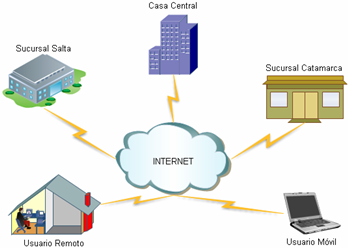
\includegraphics{imagenes/costos/esc_ej_internet}
\caption{Escenario de conexi�n a Internet de Empresa Ejemplo S.A.}
\label{fig:alternativas_vpn1}
\end{figure}

\subsection{Relevamiento}

Al realizar el relevamiento de Empresa Ejemplo S.A. se obtuvo informaci�n de la situaci�n, luego se presentaron las opciones para la soluci�n o mejora de las fallas encontradas; tambi�n se procedi� a  documentar el proceso.

\subsubsection{Equipamiento}

Se puede comenzar con el equipamiento de la casa central y las sucursales. En la casa central se cuenta con terminales \emph{Workstation HP xw8600} y dos servido\emph{HP ProLiant ML100} que se utilizan para servidor de archivos y aplicaciones, y para servicios Web y correo electr�nico. Los terminales de usuarios cuentan con el sistema operativo Microsoft Windows Vista Home Premiun preinstalado, mientras que los servidores tienen Windows Server 2007 en cada equipo.

Las otras dos sucursales, cuentan con los mismos equipos para terminales de usuarios, pero con un solo servidor HP ProLiant ML100 en cada local. Cada servidor se utiliza para la conexi�n a Internet y para el reparto de correo electr�nico local.

Los usuarios m�viles de Empresa Ejemplo S.A. generalmente se conectan a la casa central mediante la interfaz Web en busca de informaci�n para los clientes, dado que rara vez se puede utilizar la conexi�n a escritorio remoto, porque se trata de un servicio que no deber�a estar disponible en Internet las 24 horas del d�a.

\subsubsection{Comunicaciones}

En cuanto al esquema de conexi�n, la casa central cuenta con ADSL sim�trico de 3 Mbps, y las sucursales con ADSL com�n de 1 Mbps, porque no se consideraba que iba a ser necesario comunicarse entre las sucursales, nada m�s con consultar el servicio Web principal era suficiente.

Para la comunicaci�n se utilizaba un modem router ADSL provisto por el ISP (un Tainet CA81R) para los tres locales. Este aparato cumple la funci�n de NAT y de firewall para la toda la red, y se conecta a un Switch 3Com de 24 bocas en la casa central y de 16 en cada sucursal.

En algunos casos era necesario supervisar la utilizaci�n del acceso a Internet de cada empleado, ya que en determinados horarios resultaba imposible trabajar por el alto consumo de ancho de banda que tomaban las terminales con programas P2P durante las descargas.

\subsubsection{Servicios}

En la casa central se tienen servicios b�sicos de Web y correo elect�nico en un equipo, mientras que en el otro equipo se cuenta con servidor de archivos, utilizado para la documentaci�n importante de la empresa y limitado a cada usuario protegi�ndolo con contrase�a.

Si un usuario m�vil requiere de un archivo alojado en el servidor, debe solicitar mediante tel�fono o correo electr�nico que se habilite el servicio por un per�odo de tiempo limitado. Esto es para evitar ingreso de intrusos a la red, ya que es servicio de acceso a escritorio remoto se encontrar�a disponible para toda la Internet.

En las sucursales se cuentan con servicio de correo electr�nico y de archivos en un mismo equipo, ya que no hay tantos terminales conectados al mismo tiempo.

Para obtener acceso a la casa central se ha creado un formulario Web (en el servidor) en el que cada usuario puede modificar y obtener informaci�n de productos de la empresa, mediante su nombre y contrase�a. Es decir, que el sitio web utilizado por la empresa para mostrar a los clientes, tiene la misma interfaz que la que utilizan sus empleados para obtener y modificar informaci�n importante de productos y servicios.

\subsection{Problemas encontrados}

Luego de realizar el relevamiento de Empresa Ejemplo S.A. se encontraron algunos problemas en cuanto a la estructura de la red de la empresa y el manejo de informaci�n vital.

En primer lugar se tiene en cuenta que la distancia de la casa central y de las sucursales es tal que produce gran dispersi�n de la informaci�n, como si de varias empresas se trataran. La idea general es unificar este tipo de informaci�n para que la empresa se vea identificada por su casa central para mejorar la imagen corporativa.

En segundo lugar, en el acceso a la red, los empleados m�viles tienen dificultades para encontrar informaci�n precisa para distribuir a sus clientes, ya que no siempre pueden acceder a la red de la empresa, y el formulario Web es demasiado limitado para la mayor�a de los casos. Por eso es necesario establecer una pol�tica de acceso para los terminales m�viles, ya sea mediante el uso de equipos port�tiles como de tel�fonos m�vil.

Finalmente, la administraci�n de los equipos, los servicios y de la red, se hace muy dif�cil por la dispersi�n que existe en el sistema de Empresa Ejemplo S.A. Por ejemplo, el correo electr�nico de cada sucursal deber�a unificarse con el servidor central (es decir, cada sucursal tiene su correo, pero son redireccionados al servidor central), de la misma manera que el servidor de archivos, para que la seguridad sea fortalecida en un solo lugar. De esta manera se evita la redundancia de la informaci�n, que se repite en las sucursales y en la casa central, y la actualizaci�n de los mismos deben hacerse mediante copias de los archivos a cada sucursal, haciendo el trabajo menos din�mico y m�s tedioso.

\subsection{Recomendaciones}

Luego de conocer la situaci�n actual de Empresa Ejemplo S.A. se procede con el listado de recomendaciones realizadas por expertos en seguridad e infraestructura de red.

\subsubsection{Infraestructura y equipos}

En cuanto al equipamiento de Empresa Ejemplo S.A. se cuenta con equipos relativamente nuevos, tanto en las terminales como en los servidores, por lo que no es necesaria la adquisici�n de nuevas m�quina.

En la casa central y en las sucursales, se utilizan Switches y cables de buena calidad; se tiene una buena distribuci�n de los cables por sus correspondientes cable-canal. Es decir, en cuanto a materiales, se cuenta con las mejores opciones; el problema esta en la arquitectura funcional de la red y distribuci�n de servicios.

\subsubsection{Informaci�n vital}

Para proteger la informaci�n cr�tica para el funcionamiento de la empresa, se han planteado las siguientes opciones:

\begin{itemize}
	\item \emph{Opci�n 1:} Centralizar la informaci�n en la base de datos de la casa central. Instalar un servidor de backup en cada sucursal. Todos los empleados \textendash incluso los de las sucursales \textendash ingresar�n a la base de datos de la casa central para obtener la informaci�n que necesitan.
	\item \emph{Opci�n 2:} Centralizar la informaci�n en la base de datos de la casa central. Pero crear servidores espejo en ambas sucursales, para ahorrar tiempo en el acceso a los datos necesarios por los empleados.
\end{itemize}

De entre ambas opciones, se escoge la primera, ya que la segunda tiene la desventaja que al momento de la sincronizaci�n se consume mucho ancho de banda, por que la frecuencia de actualizaci�n de los servidores espejo debe ser mayor que la de los servidores backup.

\subsubsection{Servicios de red}

Crear en la casa central una \gls{DMZ}, donde se ubiquen los servicios al p�blico en general: servicio web por el momento. Quitar todos los que puedan ofrecer alg�n tipo de vulnerabilidad.

Los servicios necesarios para los empleados, como por ejemplo el servicio de correo, Web, el sistema de gesti�n, y dem�s, ser�n accedidos desde dentro de la red local, o desde una conexi�n no accesible al p�blico en general. En la Figura \ref{fig:alternativas_vpn2} vemos c�mo ser�a el esquema de red de la casa central.

\begin{figure}[htbp]
\centering
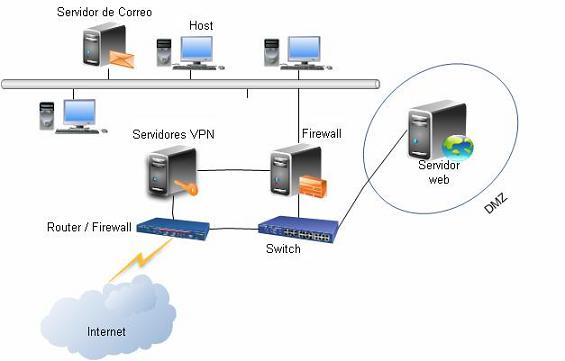
\includegraphics{imagenes/costos/esc_ej_cc}
\caption{Infraestructura de la red de la casa central.}
\label{fig:alternativas_vpn2}
\end{figure}

Las sucursales no poseer�n servicios p�blicos, estos solo se brindar�n desde la central.

\subsubsection{Conexi�n a Internet}

Cada una de los puestos fijos acceder� a Internet a trav�s de un proveedor local. La casa central debe tener direcci�n IP fija, mientras que en las sucursales esto no es necesario. 

El servidor Dynamic DNS de la central resolver� los nombres de de las sucursales (si es necesario).

\subsubsection{Conexi�n con la Casa central}

Cada una de las sucursales se comunicar�n directamente con la casa central, pero entre ellas no habr� comunicaci�n directa, ya que esto provocar�a una sobrecarga administrativa de la red, que es mayor al aprovechamiento que se le da. La conexi�n inal�mbrica no es una opci�n en este caso debido a la distancia que hay entre los lugares a comunicar, por lo que queda descartada. Las opciones son las siguientes:

\begin{itemize}
	\item \emph{Opci�n 1:} Alquilar dos l�neas, para conectar la central con cada una de las sucursales. Con esto se gana en privacidad y seguridad. 
	\item \emph{Opci�n 2:} Establecer conexiones VPN sobre las conexiones a Internet existentes, entre la central y cada una de las sucursales. El tr�fico viajar� por la red p�blica, pero encriptado; si se implementan bien los servidores VPN, no habr� mayores problemas con respecto a la seguridad.
\end{itemize}

La opci�n que se adopta, es la segunda. Debido a que, si bien la primera ofrece mayor seguridad, por otro lado es mucho m�s costosa, y posee la desventaja que si el enlace se corta en alg�n punto entre los nodos, puede haber gran retardo en restablecer la comunicaci�n.

La Figura \ref{fig:alternativas_vpn3} muestra detalles de la infraestructura de red de las sucursales.

\begin{figure}[htbp]
\centering
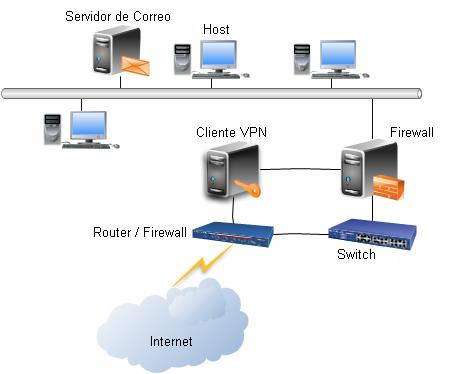
\includegraphics{imagenes/costos/esc_ej_suc}
\caption{Infraestructura de la red de las sucursales.}
\label{fig:alternativas_vpn3}
\end{figure}

\subsubsection{Empleados itinerantes y remotos}

Se hizo un estudio para averiguar cu�ntos empleados se conectaban remotamente a la casa central y cu�ntos a las sucursales. Se hall� que en la primera el m�ximo de conexiones simult�neas es de diez (en promedio), y en las sucursales es de cinco (tambi�n en promedio).

Debido a que ahora los datos estar�n centralizados en la oficina principal de la empresa, las conexiones VPN de los empleados remotos se establecer�n solo con este lugar. 

Se implementar� soporte para veinticinco conexiones VPN para usuarios remotos, simult�neamente a la central. Con esto se da un margen de cinco conexiones extra.

\subsubsection{Recursos compartidos a clientes}

Los clientes necesitan acceder a la empresa v�a web para obtener informaci�n de sus estados de cuentas, pagos, entre otra informaci�n cr�tica. Dicha informaci�n es privada, y necesita de un modo seguro de transmisi�n, para que no pueda ser obtenida por un curioso. Las opciones que se proponen son las siguientes:

\begin{itemize}
	\item \emph{Opci�n 1:} Habilitar conexiones VPN host-red para cada uno de los clientes que necesiten acceder a nuestra red de forma segura.
	\item \emph{Opci�n 2:} Aprovechando que en la DMZ hay un servidor web p�blico, y que los clientes solo necesitan acceso www, puede habilitarse soporte HTTPS en dicho servidor, esto es, tr�fico HTTP encriptado con SSL, de modo que el tr�fico de paquetes no circule en texto claro.
\end{itemize}

La mejor opci�n en este caso, es la segunda, ya que se evita una sobrecarga de conexi�nes VPN innecesarias y poco productivas, y que solo provocar�an una baja en el rendimiento de los servidores. Tambi�n se aprovecha algo que existe, de un modo muy sencillo: el servidor web p�blico.

\subsubsection{Administraci�n de las redes}

Suprimir la administraci�n de red individual de las sucursales. Establecer una administraci�n cen\-tra\-li\-za\-da de los tres puntos fijos en la casa central, para simplificar el control y mantenimiento de las redes.

Cada una de las sucursales poseer� una puerta de acceso VPN �nicamente para acceso administrativo de esta �ndole.

\subsection{Comparativa de costos}
\label{subsec:comparativa_costos}

Para realizar una comparativa de costos, antes se deben conocer las opciones disponibles para ofrecer lo mismo, pero con diferentes soluciones.

En cuanto a las opciones, no existe tanta variedad para el mismo costo de instalaci�n y mantenimiento, ya que puede variar para el tama�o de una empresa como en la complejidad de la red que se quiera implementar. Adem�s como las entidades buscan en general disminuir gastos, se optan por soluciones econ�micas que pueden estar relacionadas con software libre o con aparatos de gama media de Linksys o 3Com. Por el contrario, si la empresa puede gastar m�s dinero, entonces buscan la misma soluci�n en compa��as como Cisco.

En cuanto a los requisitos m�nimos para implementar una soluci�n VPN, no se van a incluir dentro del costo de la configuraci�n y mantenimiento de la VPN propiamente dicha, sino que se considera que es un gasto que la empresa debe asumir para poder invertir en una mejor soluci�n. De esta manera, se van a plantear solamente los costos de la instalaci�n, configuraci�n y mantenimiento de una VPN, que en algunos casos puede ir incluido con el equipamiento, pero en Empresa Ejemplo S.A. no ser� necesario porque ya disponen de equipos suficiente.

En algunos casos en los que se pretende gastar menos dinero en implementaci�n, se puede optar por soluciones h�bridas. Es decir, en la casa central se instala un equipo medianamente potente, mientras en las sucursales se opta por routers que sean compatibles con la implementaci�n de IPSec con Linux u OpenBSD.

\subsubsection{Costos de comunicaci�n}

Hace un tiempo, el reino de las comunicaciones las ten�an las l�neas telef�nicas tradicionales de cable de cobre. Luego los requerimientos fueron cambiando y las comunicaciones se volvieron inal�mbricas o satelitales, sin la intervenci�n de cables.

En la actualidad, se sigue utilizando la l�nea telef�nica tradicional pero con una nueva tecnolog�a que permit�a la conexi�n a Internet a alta velocidad, es el ADSL. De esta manera, nace una nueva alternativa a las l�neas ``dedicadas'', que se empleaban para la conexi�n de redes privadas virtuales mediante un canal independiente y de ancho de banda bajo demanda, que es la VPN a trav�s de Internet.

En cuanto a los costos de la comunicaci�n, se tiene una gran variedad de soluciones, que van desde l�neas dedicadas con \emph{framerelay} a muy alto precio, hasta la conexi�n a Internet hogare�a bastante m�s econ�mica.

Una opci�n media que se utiliza actualmente y que es la requerida en casa central de Empresa Ejemplo S.A., es el denominado \emph{ADSL sim�trico}. Esta tecnolog�a permite la misma tasa de transferencia de subida como de bajada de datos. Por ejemplo un servicio de 1 Mbps con direcciones IP fijas puede tener un costo de US\$300,00 aproximadamente, que es mucho m�s que un ADSL com�n de 5 Mbps, pero bastante menos que una l�nea dedicada, que puede superar los US\$900,00.

\subsubsection{Costos con software libre}

Como en general los clientes que solicitan un servicio requieren una soluci�n completa, en este caso, luego del relevamiento correspondiente y del an�lisis de la infraestructura de la red, no es necesario proveer de equipamiento, por lo que el costo se reducir�a solamente a la instalaci�n de los sistemas y configuraci�n de la VPN.

Los precios por la instalaci�n de un concentrador VPN con software libre, van desde los \$2.000,00 (pesos argentino) como base aproximadamente, dependiendo de la complejidad del sistema y de la importancia del tr�fico a transmitir (con respecto a la disponibilidad). Esto se mide de acuerdo a si es necesario que la VPN se encuentre activa las 24 horas del d�as, todos los d�as de la semana, etc.

En este caso, para la Empresa Ejemplo S.A. que requiere conectividad con las dem�s sucursales para realizar el backup diario, de las transferencias realizadas durante la jornada laboral, se debe tener en cuenta la disponibilidad del sistema.

De esta manera, los elementos importantes a tener en cuenta para realizar un presupuesto ser�an los siguientes:

\begin{itemize}
	\item Instalaci�n y configuraci�n del sistema (Linux u OpenBSD).
	\item Seguridad adicional por software.
	\item Disponibilidad del sistema.
	\item Cantidad de enlaces punto a punto.
	\item Soporte a usuario m�viles.
	\item Cantidad de servicios para administrar.
	\item Copias de seguridad en horarios que no se utilice el servidor.
\end{itemize}

Como los servicios que se pueden administrar son numerosos, en el siguiente listado se muestran los requeridos por Empresa Ejemplo S.A.:

\begin{itemize}
	\item Servicio Web.
	\item Servicio de Base de Datos.
	\item Servidor DNS.
	\item Servicio de correo electr�nico.
	\item Servidor de archivos.
\end{itemize}

Por consiguiente, es posible calcular el costo total, a partir del precio base, que incluye:

\begin{itemize}
	\item Configuraci�n de un enlace punto a punto (extremo servidor).
	\item Soporte a usuarios m�viles (cuya cantidad depende de la capacidad del equipo).
	\item Servidor DNS.
\end{itemize}

Al agregar los servicios Web, de correo electr�nico, base de datos y de archivos, el costo se incrementa a \$2.000,00, mientras que la configuraci�n de copias de seguridad diaria suman \$1.000,00.

Por otra parte, el tema de la disponibilidad del sistema, tiene que ver con el soporte y mantenimiento mensual de la VPN, que puede variar (dependiendo del grado de disponibilidad) entre \$1.000,00 y \$3.000,00.

La Tabla \ref{tab:costos_softlibre} muestra detalladamente el costo estimado de cada servicio junto al monto total.

\begin{table}[htb]
\begin{center}
	\begin{tabular}{l l l l l}
		\hline
		Servicio         & Cantidad & Precio Unitario & Precio total          \\
		\hline
		Instalaci�n      & 1        & \$500,00        & \$500,00              \\
		Disponibilidad   & Diario   & n.d.            & \$2.000,00            \\
		Enlaces P2P      & 2        & \$1.000,00      & \$2.000,00            \\
		M�vil            & 25       & n.d.            & \$1.000,00            \\
		Backup           & Diario   & n.d.            & \$1.000,00            \\
		Web              & 1        & \$500,00        & \$500,00              \\
		DB               & 1        & \$500,00        & \$500,00              \\
		DNS              & 1        & \$250,00        & \$250,00              \\
		E-Mail           & 1        & \$500,00        & \$500,00              \\
		Archivos         & 1        & \$250,00        & \$250,00              \\
		\hline
		Total            &          &                 & \textbf{\$8.500,00}   \\
		\hline
	\end{tabular}
\end{center}
\caption{Costos de la implementaci�n de una VPN con software libre.}
\label{tab:costos_softlibre}
\end{table}

En cuanto al costo mensual, la variaci�n del precio esta fuertemente relacionada con la disponibilidad del servicios y las copias de seguridad que se realicen. Por esta raz�n, como se ha mencionado anteriormente, el costo de mantenimiento mensual puede variar entre \$1.000,00 y \$3.000,00.

Este es el caso para la casa central. En las sucursales, el gasto siempre es menos, ya que los servicios que se administran, se encuentran en la casa central.

Para cada sucursal de Empresa Ejemplo S.A. ya se ha calculado el precio por los enlaces, por lo que solamente se suma en el precio la instalaci�n y configuraci�n del sistema, junto al mantenimiento del mismo. De esta manera se adiciona \$1.000,00 para cada servidor de cada sucursal.

De esta manera se estima que el costo total de una soluci�n VPN con software libre ser�a de \textbf{\$10.500}, que incluye el primer mes de soporte y mantenimiento. Los meses siguientes, se tendr�a que incluir el mantenimiento de la VPN, de acuerdo a la disponibilidad (que en este caso se considera una disponibilidad media), y las copias de seguridad, con un total de \textbf{\$3.000} mensuales.

\subsubsection{Costos con hardware dedicado}

En cuanto al c�lculo de una soluci�n con hardware comercial, el precio var�a solamente en el servicio de configuraci�n e instalaci�n de los equipos adquiridos. Los dem�s servicios tienen el mismo costo establecido anteriormente, es decir, se reemplaza la instalaci�n y configuraci�n del servidor VPN por la soluci�n con hardware propietario.

Para llevar a cabo esta implementaci�n, se utilizan equipos marca \emph{Cisco}, cuyos modelos y precios son los siguientes:

\begin{enumerate}
	\item Cisco ASA 5510 SSL/IPsec VPN Edition for 50 concurrent SSL VPN users (US\$ 4.500,00).
	\item 2 Cisco VPN 3002 Hardware Client (US\$ 598,00).
\end{enumerate}

El primer modelo de la lista anterior es un concentrador VPN que se utiliza como servidor para las conexiones entrantes. Permite por medio de la virtualizaci�n, a 250 sesiones concurrentes, 250 sesiones SSL y 50 usuarios concurrentes. Adem�s tiene funciones de firewall para proteger la red de ataques de hackers, malware, troyanos, e incluye bloqueo de aplicaciones P2P para evitar el intercambio de archivos.

El segundo equipo es un dispositivo que funciona en modo cliente junto al concentrador principal, estableciendo la comunicaci�n con el mismo y haciendo funciones de NAT en la red interna, que en este caso, se trata de las sucursales de Empresa Ejemplo S.A. El equipo soporta conexi�n con el ISP mediante PPPoE, adem�s de NAT transparente para IPSec. De esta manera, se puede obtener un servicio completo de conexi�n a Internet, adem�s de la conexi�n segura al servidor VPN mediante el protocolo IPSec.

Volviendo a los costos, cada equipo Cisco mencionados anteriormente, se le tienen que sumar los siguientes servicios:

\begin{itemize}
	\item Instalaci�n y configuraci�n de los equipos Cisco.
	\item Seguridad adicional por software.
	\item Disponibilidad del sistema.
	\item Cantidad de servicios para administrar.
	\item Copias de seguridad en horarios que no se utilice el servidor.
\end{itemize}

En cuanto a la seguridad adicional por hardware se refiere a la utilizaci�n de un firewall bajo OpenBSD o Linux, el cual adhiere flexibilidad a la configuraci�n y permite un mayor control de la red interna. Esto se realiza en la casa central, donde la seguridad de los equipos y la utilizaci�n de \gls{DMZ} hacen que la opci�n por software para el firewall sea la m�s indicada.

De los servicios para administrar, se incluyen los siguientes:

\begin{itemize}
	\item Servicio Web.
	\item Servicio de Base de Datos.
	\item Servidor DNS.
	\item Servicio de correo electr�nico.
	\item Servidor de archivos.
\end{itemize}

Estos servicios se implementan en casa central, pero no significa que se integra el mantenimiento del sitio Web corporativo ni el contenido de la base de datos, sino que se cuenta la instalaci�n y configuraci�n de los servicios. El tema de la migraci�n, si se utiliza un sistema diferente en aplicaciones Web y de base de datos, es un caso aparte, que requiere otro proceso de planificaci�n y por lo tanto un precio adicional. En esta situaci�n de ejemplo, se considera que el sitio Web anterior y la base de datos, son f�cil de migrar al nuevo sistema.

La Tabla \ref{tab:costos_hardware} muestra el c�lculo de costos utilizando esta soluci�n por hardware de una VPN, que adem�s se incluyen servicios con software libre.

\begin{table}[htb]
\begin{center}
	\begin{tabular}{l l l l l}
		\hline
		Servicio         & Cantidad & Precio Unitario & Precio total          \\
		\hline
		Instalaci�n      & 3        & \$300,00        & \$900,00              \\
		Disponibilidad   & Diario   & n.d.            & \$2.000,00            \\
		Cisco ASA 5510   & 1        & US\$ 4.500,00   & US\$ 4.500,00         \\
		Cisco VPN 3002   & 2        & US\$ 600,00     & US\$ 1.200,00         \\
		Backup           & Diario   & n.d.            & \$1.000,00            \\
		Web              & 1        & \$500,00        & \$500,00              \\
		DB               & 1        & \$500,00        & \$500,00              \\
		DNS              & 1        & \$250,00        & \$250,00              \\
		E-Mail           & 1        & \$500,00        & \$500,00              \\
		Archivos         & 1        & \$250,00        & \$250,00              \\
		\hline
		Total            &          &                 & \textbf{\$23.666,00}  \\
		\hline
	\end{tabular}
\end{center}
\caption{Costos de la implementaci�n de una VPN con software libre.}
\label{tab:costos_hardware}
\end{table}

Por otro lado, el costo de mantenimiento es el mismo que en el caso anterior, pero no se incluye el soporte que se pueda necesitar en los equipos Cisco, ya que para esto se requiere de agente especializados de dicha empresa. El gasto inicial total con un mes de soporte es de \textbf{\$23.666,00}, con un mensual de \textbf{\$3.000,00}.

\section{Conclusi�n}
\label{sec:alternativas_conclusion}

Elegir una soluci�n VPN adecuada no es tarea f�cil. Requiere de mucho tiempo de planificaci�n y an�lisis, ya que se trata de una inversi�n importante que puede salir muy bien o definitivamente puede ser una p�rdida de tiempo y mucho dinero. Esto ocurre, si no se toman todas las precauciones debidas ni se documenta o se entiende el problema; la inversi�n puede resultar un completo fracaso.

Por esta raz�n es que al elegir una soluci�n VPN adecuada se debe tener en cuenta una gran cantidad de factores como el econ�mico, la escalabilidad, la transparencia para los usuarios, la mejora de la imagen corporativa, la soluci�n a un problema cr�tico, etc.

En cuanto a las diferentes soluciones VPN, tanto los equipos comerciales, como las implementaciones en sistemas libres pueden ser muy buenas respecto a su funcionamiento; la diferencia se encuentra en que las implementaciones libres poseen una gran flexibilidad y precio m�s bajo en comparaci�n con las comerciales; pero estas �ltimas poseen la ventaja de la optimizaci�n del hardware para mejor funcionamiento de las VPN. 

En general, las grandes entidades, al implementar VPN para su tr�fico utilizan equipos comerciales, ya que el gasto en un buen equipo se justifica; mientras que las empresas m�s peque�as, optan por soluciones libres debido a que la cantidad de recursos con los que cuentan es menor. Es bueno remarcar que, por lo menos en este caso, menor precio no implica necesariamente menor calidad, ya que las implementaciones VPN mediante software pueden competir perfectamente en casi todos los aspectos con las comerciales; incluso siendo una mejor opci�n a igual precio, en algunos casos.


%% Conclusi�n final
%%%%%%%%%%%%%%%%%%%%%%%%%%%%%%%%%%%%%%%%%%%%%%%%%%%%%%%%
%   |-------------------------|                        %
%   |REDES PRIVADAS VIRTUALES |                        %
%   |                         |                        %
%   | Proyecto de graduaci�n  |                        %
%   |_________________________|                        %
%                                                      %
%   Autores                                            %
%   -------                                            %
%                                                      %
% * Formoso Requena, Nicol�s Federico (CX02-0239-8)    %
%     nicolasformoso@gmail.com                         %
% * Cortez, Gustavo Maximiliano (CX01-0801-9)          %
%     cmgustavo83@gmail.com                            %
%                                                      %
%   Tutores                                            %
%   -------                                            %
%                                                      %
% * Ing. Gustavo Vanetta - vanettag@gmail.com          %
% * Lic. Miguel Bazzano - miguelbazzano@gmail.com      %
%                                                      %
%%%%%%%%%%%%%%%%%%%%%%%%%%%%%%%%%%%%%%%%%%%%%%%%%%%%%%%%

% ********* Conclusi�n final  ********** %

\chapter{Conclusi�n final}
\label{chap:conclusion}

La informaci�n es lo que da vida a una empresa, por tanto, es importante que sea resguardada. Esto implica que deber�n tomarse las medidas necesarias para que cuando haya que transmitirla entre sucursales, empleados, etc, no sea expuesta al mundo exterior, ya que si la informaci�n corre riesgo, se compromete la vida de la entidad. Por esto, mientras mayor sea el riesgo, mayor ser� la justificaci�n del gasto en la seguridad de nuestros datos. 

Teniendo en cuenta lo anterior, una empresa grande optar� por soluciones como l�neas dedicadas, enlaces inal�mbricos o MPLS, para el tr�fico m�s cr�tico; e implementaciones de redes privadas virtuales para el tr�fico de menor importancia.
Ahora si se trata del mismo caso, pero en una empresa mediana o peque�a, que posee menos recursos, probablemente la implementaci�n de VPNs ser� la �ptima.

En materia de redes privadas virtuales no existe la certeza de que utilizar lo m�s nuevo o lo considerado m�s ``seguro'', sea la mejor soluci�n para una empresa. Aunque, en principio, la mayor�a de los sistemas VPN funcionan de forma similar, en realidad, la diferencia entre ellos es lo suficientemente significativa como para elegir uno sobre otro. Antes de hacer una opci�n hay que analizar las variables m�s importantes: cu�n delicada es la informaci�n que se transmitir� a trav�s de la VPN, disponibilidad necesaria de la conexi�n, ancho de banda requerido, etc. 

Con respecto a cu�n delicados son nuestros datos, no es lo mismo la necesidad que tiene un banco que maneja dinero a trav�s de sus redes, que la que tiene un servidor de juegos online. No tiene sentido pasarse d�as, semanas o hasta meses configurando (y entendiendo) el protocolo \gls{IPSec} si solo se va a utilizar la red para transferir m�sica o compartir juegos en l�nea. Algunas alternativas, permiten con poco esfuerzo y pocas horas hombre, obtener una red privada virtual segura, confiable y r�pida. 

No obstante, a la hora de implementar una VPN \textendash y como ya vimos\textendash, la primera opci�n que debemos hacer es: hardware dedicado (cajas negras) o software implementado en un ordenador.

Las empresas dedicadas a ofrecer soluciones para redes como Cisco, 3Com, SSH.com, entre otras, brindan servicios y equipos de muy alto rendimiento, pero de elevado costo en comparaci�n con las alternativas libres. Dichos equipos no tienen \textendash en la mayor�a de los casos\textendash\hspace{0.01cm} una configuraci�n flexible, por lo que si la necesidad de conexi�n de la empresa var�a en cuanto a configuraci�n, protocolos, n�mero de conexiones, etc, y el equipo adquirido no brinda soporte para ello, ser� necesario invertir en otro nuevo. En estos casos se cumple la regla: ``A menor costo, menor flexibilidad, escalabilidad, etc.''.

En cuanto a las soluciones VPN mediante software implementadas en sistemas libres, podemos decir que en materia de seguridad, est�n muy bien dotadas, ya que cuentan con los m�s avanzados sistemas de autenticaci�n, encriptaci�n y encapsulaci�n, por lo que en dicho �mbito pueden competir perfectamente con las soluciones comerciales.
En cuanto a flexibilidad, las soluciones mediante software son las que llevan la delantera; estas brindan la posibilidad de configurar los servidores VPN en todos los aspectos posibles, implementar firewalls exclusivos para el tr�fico VPN sin invertir en hardware adicional, y si la red est� bien dise�ada, la escalabilidad se convierte en algo muy sencillo de llevar a cabo.

Puede decirse que el costo de la implementaci�n de una VPN con sistemas libres es mayor al costo que tiene la implementaci�n con hardware dedicado; esto se debe a que la instalaci�n y configuraci�n del servidor VPN por software, en el peor de los casos se hace desde cero, en cambio un equipo comercial, solo requiere ser conectado y configurado.
Si bien es cierto que el costo de la implementaci�n de una VPN en sistemas libres es mayor, hay otros par�metros a tener en cuenta que equilibran la situaci�n: la flexibilidad que obtenemos con sistemas libres, no la encontraremos en los equipos comerciales econ�micos, ni en los de un rango medio; y la segunda, es que comprar un servidor VPN comercial es m�s caro que comprar un buen ordenador, o mejor a�n, que reutilizar el hardware que ya poseemos.

Cuando nuestra opci�n para las comunicaciones son las redes privadas virtuales, y nuestro tr�fico encriptado viajar� entre los destinos atravesando Internet, debemos saber que, sea cual fuere nuestra elecci�n (si equipos comerciales, o servidores por software), el rendimiento de las comunicaciones ser� poco predecible, y depender� mucho del ancho de banda que hayamos contratado con nuestro ISP.
Es por esto, que muchas empresas optan por una conexi�n de salida a Internet para el tr�fico normal, y otra exclusiva para las conexiones VPN. Esta es otra de las cuestiones importantes a analizar.

Finalmente se puede concluir que a la hora de elegir una soluci�n VPN no solo se tiene que pensar soluciones comerciales de empresas como Cisco, Lucent, etc, sino tambi�n en las alternativas libres. Ya que estas tienen para ofrecernos grandes ventajas: bajo costo, gran flexibilidad (al punto de adaptarse perfectamente a la necesidad real), alto grado de seguridad y escalabilidad en nuestras redes.


%% Apendice
%%%%%%%%%%%%%%%%%%%%%%%%%%%%%%%%%%%%%%%%%%%%%%%%%%%%%%%%
%   |-------------------------|                        %
%   |REDES PRIVADAS VIRTUALES |                        %
%   |                         |                        %
%   | Proyecto de graduaci�n  |                        %
%   |_________________________|                        %
%                                                      %
%   Autores                                            %
%   -------                                            %
%                                                      %
% * Formoso Requena, Nicol�s Federico (CX02-0239-8)    %
%     nicolasformoso@gmail.com                         %
% * Cortez, Gustavo Maximiliano (CX01-0801-9)          %
%     cmgustavo83@gmail.com                            %
%                                                      %
%   Tutores                                            %
%   -------                                            %
%                                                      %
% * Ing. Gustavo Vanetta - vanettag@gmail.com          %
% * Lic. Miguel Bazzano - miguelbazzano@gmail.com      %
%                                                      %
%%%%%%%%%%%%%%%%%%%%%%%%%%%%%%%%%%%%%%%%%%%%%%%%%%%%%%%%

% ********* Ap�ndices ********** %

\appendix

%%%%%%%%%%%%%%%%%%%%%%
% Equipos de prueba  %
%%%%%%%%%%%%%%%%%%%%%%

\chapter{Equipos de prueba}
\label{appendix:equipos_de_prueba}

En este Ap�ndice se detallan las caracter�sticas de las redes y equipos utilizados para las pruebas durante el desarrollo del proyecto. La intensi�n del mismo es proveer informaci�n de los requisitos m�nimos del hardware necesario para obtener resultados similares (o superiores) a los que se han podido llegar.

Adem�s se plantean los esquemas de conexi�n a nivel general que cada red utiliza para el acceso a Internet, que por su parte, se profundiza en el Cap�tulo \ref{chap:ConexionAInternet} de la p�gina \pageref{chap:ConexionAInternet}.

\section{Ambiente de trabajo}
\label{appendix:ambiente_de_trabajo}

Debido a que la naturaleza del proyecto as� lo requiere, para las pruebas, se utilizaron dos redes \gls{LAN} distantes. La comunicaci�n entre ellas se realiza a trav�s de la red p�blica (Internet). Las redes locales se describen m�s adelante en las secciones \ref{appendix:red_1} y \ref{appendix:red_2} de las p�ginas \pageref{appendix:red_1} y \pageref{appendix:red_2} respectivamente.

Cada red se conecta a su ISP (Internet Service Provider), el cual provee un entorno de comunicaci�n ideal en cuanto a cantidad de tr�fico e informaci�n que circula por la misma, de manera que se puede tener un entorno real de comunicaci�n por un medio inseguro entre las dos redes locales. Un esquema simplificado, que muestra la conexi�n l�gica entre las redes, se puede ver en la Figura \ref{fig:enlace_logico}.

\begin{figure}[htb]
	\centering
	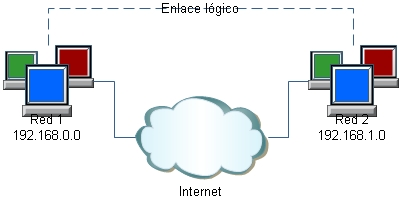
\includegraphics{imagenes/general/enlace_logico}
	\caption{Conexi�n a Internet de ambas redes y el enlace l�gico creado por la VPN.}
	\label{fig:enlace_logico}
\end{figure}

Ambas redes locales utilizan, para el tr�fico de datos, el protocolo de capa dos \gls{Ethernet} y el conjunto de protocolos TCP/IP. Esto hace que no sean necesarias aplicaciones o dispositivos de conversi�n entre dos o m�s protocolos, dejando esta tarea para que la realicen los respectivos sistemas operativos.

\section{Red \texttt{casa.lan}}
\label{appendix:red_1}

Esta subred cuenta con tres hosts interconectados entre s� por un router que posee funciones de switch y WAP (Wireless Access Point).

El rango de direcciones IP que se utiliza es \texttt{192.168.1.0/24}, es decir, de la direcci�n \texttt{192.168.1.1} a la direcci�n \texttt{la 192.168.1.254}.

El rango \texttt{192.168.1.1} a \texttt{192.168.1.9} est� reservado para direcciones asignadas est�ticamente, y el rango \texttt{192.168.1.10} a \texttt{192.168.1.254}, se asigna din�micamente a hosts clientes por DHCP.

En la tabla \ref{tab:tabla_red1} se resumen las caracter�sticas de hardware de los equipos de la red:

\begin{table}[htb]
\centering
\begin{tabular}{l l l l l l}
	\hline
	Hostname & Direcci�n IP & Arquitectura & Memoria & Disco & Sistema Operativo\\
	\hline
	Agnus 	 & 192.168.1.2 	& x86 201Mhz  & 128MB & 6GB+20GB & OpenBSD\\
	Poncho 	 & 192.168.1.3 	& x86 1600Mhz & 256MB & 160GB 	 & WindowsXP\texttrademark\\
				   &						  &				      &		    &				   & y Ubuntu Server\\
	Notebook & Din�mica 	  & x86 1800Mhz & 512MB & 120GB 	 & WindowsXP\texttrademark\\
	\hline
\end{tabular}
\caption{Res�men de las caracter�sticas de los hosts de casa.lan}
\label{tab:tabla_red1}
\end{table}

\subsection{Descripci�n de equipos}
\label{sec:descrip_red1}

A continuaci�n se describen las caracter�sticas m�s importantes de los equipos involucrados.

\subsubsection{Modem/Router Aztech DSL600EW}

Este equipo posee 4 puertos Lan (RJ45), 1 puerto Wan (RJ11), WAP (Wireless Access Point). Conecta y permite el tr�fico de datos entre los hosts de esta red.

Brinda servicios de DHCP. Y posee funciones de \texttt{bridge} \footnote{Tanto este dispositivo como los dem�s, poseen otras funcionalidades.}.

Tiene asignada la direcci�n IP \texttt{192.168.1.1}.

\subsubsection{Hostname: agnus}

Este host establece una conexi�n pppoe con el ISP, y brinda acceso a internet a la red. Cumple tambi�n funciones de servidor DNS, SSH y VPN. A seguir, su descripci�n detallada:

\begin{tabbing}
	\hspace*{.4\textwidth} \= \hspace*{\textwidth}\kill    % define los espacios de los tabuladores
	\textbf{Procesador:} \> Cyrix 6x86MX 201 MHz\\
	\textbf{Memoria RAM (real):} \> 133787648 (127MB)\\
	\textbf{Disco R�gido 1:} \> 6105MB \\
	\textbf{Disco R�gido 2:} \> 19092MB\\
	\textbf{Sistema Operativo:} \> OpenBSD 4.2\\
	\\
	\textbf{Adaptador de Red 1:} \> 3Com 3c905B 100Base-TX\\
	\textbf{Direcci�n de Hardware (Mac):} \> 00:50:04:7c:b3:e7\\
	\textbf{Direcci�n IP:} \> 192.168.1.2\\
	\textbf{M�scara de Red:} \> 255.255.255.0\\
	\\
	\textbf{Adaptador de Red 2:} \> NE2000 (RTL8019)\\
	\textbf{Direcci�n de Hardware (Mac):} \> --\\
	\textbf{Direcci�n IP:} \> (no tiene) \\
	\textbf{M�scara de Red:} \> --\\
\label{tab:desc_agnus}
\end{tabbing}

\subsubsection{Hostname: poncho}

Este host funciona solo como cliente. A seguir, su descripci�n detallada:

\begin{tabbing}
	\hspace*{.4\textwidth} \= \hspace*{\textwidth}\kill  %define los espacios de las columnas (40% 1ra y el resto 2da)
	\textbf{Procesador:} \> x86 Family AuthenticAMD ~1599 MHz\\
	\textbf{Memoria RAM (real):} \> 256 MB\\
	\textbf{Disco R�gido:} \> 153,38 GB\\
	\textbf{Sistema Operativo:} \> Microsoft\textregistered\hspace{0.1cm} Windows XP\texttrademark\hspace{0.1cm} Professional\\
	\\
	\textbf{Adaptador de Red 1:} \> VIA Rhine II Fast Ethernet Adapter\\
	\textbf{Direcci�n de Hardware (Mac):} \> 00:14:2A:E4:21:01\\
	\textbf{Direcci�n IP:} \> 192.168.1.3\\
	\textbf{M�scara de Red:} \> 255.255.255.0\\
\label{tab:desc_poncho}
\end{tabbing}

\subsubsection{Hostname: notebook}

Este host funciona solo como cliente. A seguir, su descripci�n detallada:

\begin{tabbing}
	\hspace*{.4\textwidth} \= \hspace*{\textwidth}\kill  %define los espacios de las columnas (40% 1ra y el resto 2da)
	\textbf{Procesador:} \>  x86 Family AuthenticAMD ~1808 MHz\\
	\textbf{Memoria RAM (real):} \> 512 MB \\
	\textbf{Disco R�gido:} \> 120 GB\\
	\textbf{Sistema Operativo:} \> Microsoft\textregistered\hspace{0.1cm} Windows XP\texttrademark\hspace{0.1cm} Professional\\
	\\
	\textbf{Adaptador de Red 1:} \> WLAN Broadcom 802.11b/g\\
	\textbf{Direcci�n de Hardware (Mac):} \> 00:1A:73:5D:AE:79\\
	\textbf{Direcci�n IP:} \> (din�mica)\\
	\textbf{M�scara de Red:} \> --\\
\label{tab:desc_notebook}
\end{tabbing}

\section{Red \texttt{red.lan}}
\label{appendix:red_2}

Esta red esta compuesta por cuatro computadoras que cumplen diferentes funciones dentro de un entorno hogare�o. Las funciones que cumplen son diversas, comenzando por un servidor de acceso a Internet para la red local, y terminando en estaciones de trabajo y ocio familiar.

Las caracter�sticas resumidas de las computadoras con sus respectivos nombres para identificarlas se pueden ver en la Tabla \ref{tab:tabla_red2}. Las caracter�sticas m�s detalladas se pueden ver en \ref{subsec:descrip_red2}.

\begin{table}[htb]
\begin{center}
	\begin{tabular}{l l l l l l}
		\hline
		Hostname     & Direcci�n IP & Arquitectura & Memoria & Disco   & Sistema Operativo            \\
		\hline
		superhijitus & 192.168.0.1  & x86 166Mhz   & 95MB    & 4134MB  & OpenBSD                      \\
		wasa         & 192.168.0.2  & x86 866Mhz   & 256MB   & 40020MB & Ubuntu Server                \\
		nippur       & Din�mica     & x86 1.9Ghz   & 1024MB  & 488.3GB & Windows Vista\texttrademark  \\
		supermaquina & Din�mica     & x86 3GHz     & 512MB   & 80GB    & Windows XP\texttrademark     \\
		\hline
	\end{tabular}
\end{center}
\caption{Res�men de las caracter�sticas de los hosts de red.lan}
\label{tab:tabla_red2}
\end{table}

\subsection{Descripci�n de equipos}
\label{subsec:descrip_red2}

A continuaci�n una descripci�n m�s detallada de los equipos involucrados.

\subsubsection{Modem/Router ADSL (modo bridge)}

Este equipo realiza la conexi�n a Internet propiamente dicha mediante un puente entre la LAN y la WAN del proveedor. Marca y modelo del dispositivo es: \emph{Amigo Tainet CA81R}.

\subsubsection{Switch 3COM (8 bocas)}

Este dispositivo permite conectar entre s� a varios clientes de la red y as� tambi�n compartir el acceso a Internet. A seguir, su descripci�n detallada:

\subsubsection*{\textit{Hostname: superhijitus}}

\begin{tabbing}
	\hspace*{.4\textwidth} \= \hspace*{\textwidth}\kill
	\textbf{Procesador:} \> Intel Pentium (P54C) (GenuineIntel 586-class) 166 MHz\\
	\textbf{Memoria RAM (real):} \> 100233216 (95MB)\\
	\textbf{Disco R�gido:} \> 4134MB\\
	\textbf{Sistema Operativo:} \> OpenBSD 4.3 (GENERIC)\\
	\\
	\textbf{Adaptador de Red 1:} \> Realtek 8139\\
	\textbf{Direcci�n de Hardware (MAC):} \> 00:08:54:b2:48:b6\\
	\textbf{Direcci�n IP:} \> 192.168.0.1\\
	\textbf{M�scara de Red:} \> 255.255.255.0\\
	\\
	\textbf{Adaptador de Red 2:} \> NE2000 (RTL8019)\\
	\textbf{Direcci�n de Hardware (MAC):} \> 00:c0:df:ab:2e:f1\\
	\textbf{Direcci�n IP:} \> (no tiene)\\
	\textbf{M�scara de Red:} \> (no tiene)\\
	\\
	\textbf{Adaptador de Red 3:} \> NE2000 (RTL8019)\\
	\textbf{Direcci�n de Hardware (MAC):} \> 00:c0:df:ab:0b:e9\\
	\textbf{Direcci�n IP:} \> (no tiene)\\
	\textbf{M�scara de Red:} \> (no tiene)\\
\end{tabbing}

\subsubsection{Hostname: wasa}

Equipo servidor utilizado para proveer de acceso \gls{PPTP}, OpenVPN, entre otros. A seguir, su descripci�n detallada:

\begin{tabbing}
	\hspace*{.4\textwidth} \= \hspace*{\textwidth}\kill
	\textbf{Procesador:} \> Intel Pentium III (866 Mhz)\\
	\textbf{Memoria RAM (real):} \> 256 MB\\
	\textbf{Disco R�gido:} \> 40020 MB\\
	\textbf{Sistema Operativo:} \> Ubuntu 8.04 LTS\\
	\\
	\textbf{Adaptador de Red 1:} \> RealTek RTL8139\\
	\textbf{Direcci�n de Hardware (Mac):} \> 00:08:54:a4:0a:62\\
	\textbf{Direcci�n IP:} \> 192.168.0.2\\
	\textbf{M�scara de Red:} \> 255.255.255.0\\
	\\
	\textbf{Adaptador de Red 1:} \> RealTek RTL8139\\
	\textbf{Direcci�n de Hardware (Mac):} \> 00:08:54:a4:0a:6e\\
	\textbf{Direcci�n IP:} \> (no tiene)\\
	\textbf{M�scara de Red:} \> (no tiene)\\
\end{tabbing}

\subsubsection{Hostname: nippur}

Equipo de escritorio que solo cumple funciones de cliente, salvo cuando se realizan pruebas con \gls{PPTP}. A seguir, su descripci�n detallada:

\begin{tabbing}
	\hspace*{.4\textwidth} \= \hspace*{\textwidth}\kill
	\textbf{Procesador:} \> AMD Athlon(tm) X2 Dual Core BE2300, 1900 Mhz\\
	\textbf{Memoria RAM (real):} \> 1 GB\\
	\textbf{Disco R�gido:} \> 500 GB\\
	\textbf{Sistema Operativo:} \> Microsoft\textregistered\hspace{0.1cm} Windows Vista\texttrademark\hspace{0.1cm} Home Premium\\
	\\
	\textbf{Adaptador de Red 1:} \> NVIDIA nForce Networking Controller\\
	\textbf{Direcci�n de Hardware (Mac):} \> 00:1E:90:22:26:1C\\
	\textbf{Direcci�n IP:} \> (din�mica)\\
	\textbf{M�scara de Red:} \> (din�mica)\\
\end{tabbing}

\subsubsection{Hostname: supermaquina}

Servidor que se conecta a Internet y provee del nombre de usuario y contrase�a al ISP. Este equipo es el que asigna direcciones IP din�mica a los clientes y permite el acceso a Internet mediante NAT a toda la red local. A seguir, su descripci�n detallada:

\begin{tabbing}
	\hspace*{.4\textwidth} \= \hspace*{\textwidth}\kill
	\textbf{Procesador:} \> Intel Pentium 4 630, 3.0 Ghz\\
	\textbf{Memoria RAM (real):} \> 512 MB\\
	\textbf{Disco R�gido:} \> 80 GB\\
	\textbf{Sistema Operativo:} \> Microsoft\textregistered\hspace{0.1cm} Windows XP\texttrademark\hspace{0.1cm} Professional\\
	\\
	\textbf{Adaptador de Red 1:} \> Networking Controller\\
	\textbf{Direcci�n de Hardware (Mac):} \> 00:13:8f:48:a2:cf\\
	\textbf{Direcci�n IP:} \> (din�mica)\\
	\textbf{M�scara de Red:} \> (din�mica)\\
\end{tabbing}

\chapter{Documentaci�n}
\label{appendix:documentacion}

Para la realizaci�n del informe de esta tesis se utilizaron una serie de herramientas que facilitaron la organizaci�n, escritura y formato del resultado final del mismo.

La finalidad de utilizar software libre para el procesamiento de la documentaci�n, fue el de tener f�cil acceso al c�digo fuente,  permitiendo la visualizaci�n desde cualquier editor de texto y adem�s de generar archivos con formato PDF que se ha convertido en  est�ndar ISO para la impresi�n en papel y en pantalla de cualquier tipo de documento. Por esta raz�n se ha utilizado, para el proceso de ``compilaci�n'', el software de composici�n de documentos profesionales Latex, que permite una terminaci�n m�s profesional en lo que respecta al formato de la documentaci�n. La Figura \ref{fig:piramide_latex} muestra la pir�mide de componentes m�s importantes de Latex para generar el documento, en el que se destaca como elemento central al repositorio de paquetes adicionales de CTAN\footnote{Comprehensive TeX Archive Network, o Red de Archivos TeX comprensibles}, que permite incluir gran cantidad de funciones adicionales y est�ndar del lenguaje.

\begin{figure}[htbp]
	\centering
		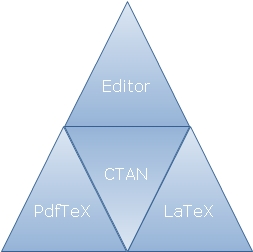
\includegraphics{imagenes/general/piramide_latex}
	\caption{Pir�mide uniforme de los componentes principales para generar documentos Latex.}
	\label{fig:piramide_latex}
\end{figure}

En las siguientes secciones se describen con m�s detalles las herramientas utilizadas, que van de los editores de texto a los paquetes de software de Latex y una breve descripci�n del mismo. Adem�s se hace menci�n a los m�todos de trabajo en equipo mediante el uso del software \gls{Subversion} para el control de versiones de la documentaci�n y en la organizaci�n de la estructura b�sica del informe.

\section{Herramientas de edici�n}
\label{appendix:herramientas_de_edicion}

Para la edici�n de la tesis se han utilizado herramientas de composici�n de textos que permitieron una salida por pantalla e impresi�n elegantes y a su vez de car�cter profesional y estructurado. El autor principal de generar esta documentaci�n es Latex, que es software libre bajo licencia LPPL, por lo que resulta ideal para el prop�sito de realizar una tesis de grado.

Las herramientas que m�s cambiaron durante la investigaci�n fueron los editores de texto, ya que a medida que iban surgiendo las necesidades, se probaban software de diferentes desarrolladores hasta encontrar la conformidad. El siguiente listado muestra los paquetes de software utilizados alguna vez durante el proceso de documentaci�n:

\begin{itemize}
	\item pdfTeX, Version 3.141592-1.40.4 (MiKTeX 2.7)
	\item LEd (Latex EDitor)
	\item TeX Maker 1.7
	\item TeXnicCenter 1 beta 7.50
	\item Emacs 22
\end{itemize}

El primer �tem es el compilador de Latex propiamente dicho, que se encarga de generar directamente la salida en formato PDF, y adem�s toma las im�genes en formatos PNG, JPG, entre otros que no sean vectoriales.

\subsection{Compilador de \LaTeX}

\LaTeX es un lenguaje demarcado para documentos, formado por un gran conjunto de macros de TeX que fueron escritos inicialmente por Leslie Lamport en 1984, con la intenci�n de facilitar el uso del lenguaje de composici�n tipogr�fica creado por Donald Knuth. Es muy utilizado para la composici�n de art�culos acad�micos, tesis y libros t�cnicos, dado que la calidad tipogr�fica de los documentos realizados con LaTeX es comparable a la de una editorial cient�fica de primera l�nea.

Este compilador de documentos se puede utilizar mediante la l�nea de comandos o a trav�s del mismo software de edici�n que incorpora los comandos necesarios para generar el archivo DIV, PDF o PS seg�n sea cada caso. La siguiente l�nea de c�digo muestra la salida al ejecutar ``pdftex'' en una terminal de Windows:

\begin{listing}[style=consola, numbers=none]
Microsoft Windows [Versi�n 6.0.6001]
Copyright (c) 2006 Microsoft Corporation.  Reservados todos los derechos.

C:\Users\Gustavo>pdftex
This is pdfTeX, Version 3.141592-1.40.4 (MiKTeX 2.7)
**
\end{listing}

Luego solicita ingresar el nombre del archivo .tex a compilar. Si no se ingresa ninguno, devuelve mensajes de error.

El uso de esta terminal suele ser muy complicado y dif�cil de controlar, depurar c�digo, etc. Para esto es m�s recomendado utilizar el nombre del archivo .tex luego del comando ``pdftex'' o bien dejar este proceso en manos de un IDE espec�fico para documentos Latex.

La filosof�a de trabajo de \LaTeX es un tanto diferente a la de los procesadores de texto habituales (conocidos como WYSIWYG, es decir, lo que ves es lo que obtienes); dicha filosof�a se basa en comandos como se ha mencionado anteriormente. Este modo de trabajo permite a quien escribe un documento, centrarse exclusivamente en el contenido y sin tener que preocuparse de los detalles del formato de salida.

Por otro lado Latex ofrece independencia del dispositivo (impresora, pantalla, etc.) o del sistema operativo (Windows, MacOS, Unix, Linux, etc.) en el que se haya compuesto el documento, permitiendo adem�s exportar a los formatos:

\begin{itemize}
	\item Postscript,
	\item PDF,
	\item SGML,
	\item HTML,
	\item RTF,
	\item entre otros.
\end{itemize}

El formato que se ha utilizado para la realizaci�n de esta tesis es PDF, ya que es el m�s extendido de todos y su visualizador oficial de Adobe se puede ejecutar en cualquier plataforma.

\subsection{Edici�n con TeXnicCenter}

Una de las herramientas que mejor se ha adaptado a la edici�n, depuraci�n y composici�n de la documentaci�n fue el software libre \index{TeXnicCenter} versi�n 1 beta 7.50 (Figura \ref{fig:texniccenter}). Este posee numerosas caracter�sticas que hacen m�s f�cil la escritura y organizaci�n de la tesis de grado, tales como:

\begin{itemize}
	\item Resaltado de sintaxis,
	\item Barra de herramientas con formatos r�pidos,
	\item Acceso directo a la ecuaciones b�sicas,
	\item Teclas de acceso r�pido a la compilaci�n y previsualizaci�n del documento,
	\item Botones de navegaci�n por los errores de sintaxis, advertencias y errores de margenes,
	\item Posibilidad de incluir diccionarios de espa�ol para la correcci�n ortogr�fica,
	\item Entre otros.
\end{itemize}

Una de las caracter�sticas pobres de este editor son los modos de navegaci�n por los cap�tulos y secciones de la documentaci�n. Y a pesar de que se pueden crear proyectos con estas caracter�sticas, se pierde la independencia en el uso de cualquier editor de texto que mejor se adapte a los gustos y necesidades de cada uno. Por esta raz�n, no se crean proyectos con ning�n editor Latex para evitar introducir archivos propios de cada software.

\begin{figure}[htbp]
	\centering
		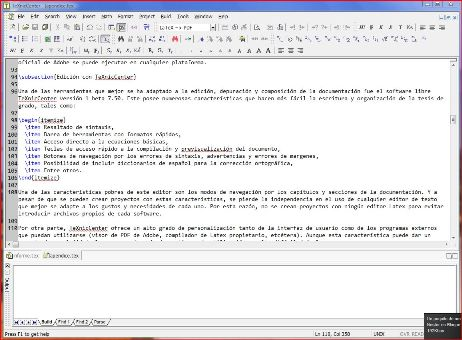
\includegraphics{imagenes/texniccenter}
	\caption{Interfaz de usuario ligeramente modificada, pero manteniendo su simpleza.}
	\label{fig:texniccenter}
\end{figure}

Por otra parte, TeXnicCenter ofrece un alto grado de personalizaci�n tanto de la interfaz de usuario como de los programas externos que puedan utilizarse (visor de PDF de Adobe, compilador de Latex propietario, etc). Aunque esta caracter�stica puede dar un aspecto de complejidad al programa, despu�s de un tiempo de utilizaci�n resulta dif�cil dejarlo.

\subsection{Edici�n con TexMaker}

Otra de las herramientas de edici�n de documentos Latex es TexMaker (Figura \ref{fig:texmaker}), que se caracteriza por la amigable interfaz de usuario, con iconos grandes y colores llamativos. Este software libre hace que la experiencia escribiendo la tesis de grado sea realmente agradable y sin nada que envidiar a los procesadores de textos actuales.

\begin{figure}[htbp]
	\centering
		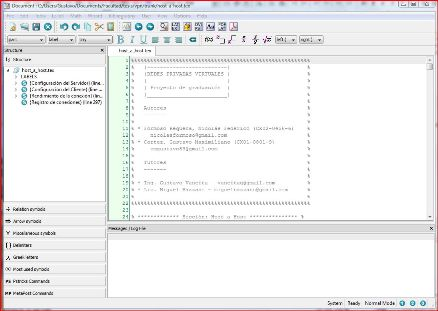
\includegraphics{imagenes/texmaker}
	\caption{TeXMaker y su agradable interfaz de usuario, durante la edici�n de esta tesis.}
	\label{fig:texmaker}
\end{figure}

TeXMaker tiene muchas caracter�sticas interesantes que ayudan a la escritura de documentos Latex, entre ellas se listan a continuaci�n:

\begin{itemize}
	\item Resaltado de sintaxis,
	\item Autocompletado de los comandos predefinidos,
	\item Muestra las referencias del archivo abierto (como un navegador de cap�tulos, secciones, etc.),
	\item Entre otros.
\end{itemize}

\subsection{Edici�n con LEd}

LEd (de Latex Editor) es un software gratuito que permite la edici�n de documentos Latex con previsualizaci�n incorporada si se esta trabajando con formato DVI. El entorno visual es muy completo y ofrece la mayor�a de los botones de acceso directo a las operaciones m�s utilizadas en la barra de herramientas, como se puede observar en la Figura \ref{fig:led}.

\begin{figure}[htbp]
	\centering
		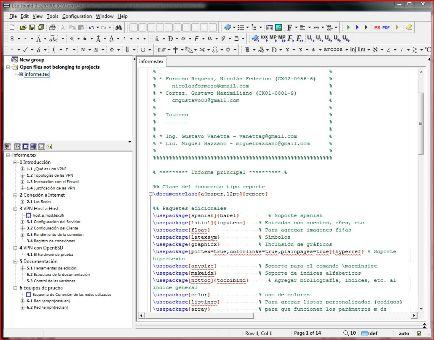
\includegraphics{imagenes/led}
	\caption{Entorno de edici�n LEd sin la vista previa activada.}
	\label{fig:led}
\end{figure}

Las caracter�sticas m�s destacadas de LEd se listan a continuaci�n:

\begin{itemize}
	\item Resaltado de sintaxis,
	\item Autocompletado de los comandos Latex m�s importantes,
	\item Previsualizaci�n instant�nea del documento en DVI,
	\item Gran cantidad de botones con funciones r�pidas para Latex,
	\item Entre otros.
\end{itemize}

LEd es software gratuito, pero existe una versi�n comercial con soporte t�cnico incluido. Para el prop�sito de esta tesis, se utiliza la versi�n gratuita que es m�s que suficiente.

\subsection{Diagramas con Edraw Max}

Edraw Max es un software comercial que se utiliza para hacer todo tipo de diagramas, que van desde el dise�o de viviendas (simples) hasta los diagramas UML, electr�nicos y de red, entre varios otros modelos. Adem�s incluye una serie de ejemplos para cada tipo de diagramas, lo que facilita el dise�o y muestra un panorama general del potencial del programa.

Las caracter�sticas m�s destacadas de la versi�n 4.0 son las siguientes:

\begin{itemize}
	\item Gran cantidad de modelos predefinidos de alta calidad;
	\item Interfaz similar a la de Microsoft Office 2007;
	\item Permite exportar el diagrama a varios formatos, entre ellos PDF y PNG;
	\item Posibilidad de importar modelos o gr�ficos;
	\item Diagramas de ejemplo para todos los casos.
\end{itemize}

Esta versi�n de Edraw Max se ha conseguido mediante el sitio web Give Away of the Day\footnote{http://giveawayoftheday.com}, que ofrece diariamente programas comerciales de forma gratuita por un d�a. Una captura de pantalla se puede ver en la Figura \ref{fig:edrawmax}.

\begin{figure}[htbp]
	\centering
		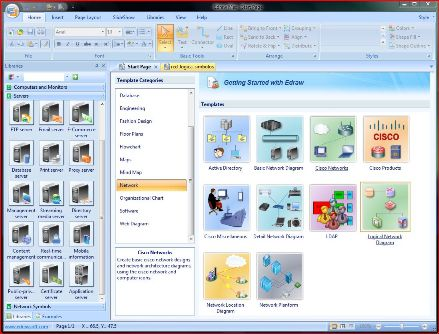
\includegraphics{imagenes/edrawmax}
	\caption{Atractiva interfaz de usuario de Edraw Max 4.0.}
	\label{fig:edrawmax}
\end{figure}

\section{Estructura de la documentaci�n}
\label{appendix:doc_estructura_documentacion}

Para que la realizaci�n de esta tesis de grado sea lo m�s organizada posible, antes de comenzar a pasar las notas, experiencias y pruebas, se detallaron las normas a seguir en cuanto a la estructura de la documentaci�n. De esta manera, se plantearon inicialmente los puntos claves que se iban incluyendo a medida que avanzaba la investigaci�n.

En esta secci�n se describen en detalles los par�metros de configuraci�n del documento Latex y los motivos de su utilizaci�n. Adem�s se incluye el esquema de la tesis y su forma de escritura.

\subsection{Definiendo el esquema}

La estructura de la documentaci�n cuenta con cap�tulos, secciones y subsecciones que permiten la ubicaci�n r�pida de determinadas tem�ticas que se incluyen como trabajo de esta tesis. Adem�s se utilizan archivos separados para disminuir el tiempo de actualizaci�n del contenido, y con las mismas ventajas que ofrece la programaci�n modular.

De esta manera se han separado l�gica y f�sicamente los archivos de cada cap�tulo de la siguiente manera:

\begin{description}
	\item[informe.tex] Contiene las definiciones de formato de salida del documento e incluye todos los cap�tulos.
	\item[nota\_facultad.tex] Es un documento independiente con la nota que se presenta para la aprobaci�n del proyecto.
	\item[apendice.tex] Herramientas utilizadas para las pruebas y redacci�n del informe final.
	\item[bibliografia.tex] Libros, revistas, sitios web o cualquier otro material al que se haya recurrido durante el aprendizaje del tema y realizaci�n de la tesis.
\end{description}

Un punto importante a destacar es la organizaci�n de los cap�tulos, que se realizan en archivos separados que no est�n incluidos en el listado anterior, pero se encuentran incluidos en el archivo \emph{informe.tex}.

\subsection{El Pre�mbulo}

El pre�mbulo es una secci�n especial de \LaTeX, donde se definen todas las directivas generales del documento, utilizadas en tiempo de compilaci�n; esta secci�n est� comprendida entre el inicio del archivo principal .tex, y la sentencia \emph{\\begin{document}}. Luego, todo lo que se encuentre entre las siguientes cl�usulas, pertenece al documento propiamente dicho.

\begin{verbatim}
\begin{document}
...
\end{document}
\end{verbatim}

Como Latex se encarga del formato del documento de salida, se ha considerado importante incluir el encabezado principal, con comentarios de cada l�nea para demostrar lo que hace cada paquete incluido.

\begin{codigo}
\begin{listing}[style=TeX]
\documentclass[a4paper,12pt]{report}
\usepackage[spanish]{babel}
\usepackage[latin1]{inputenc}
\usepackage{float}
\usepackage{latexsym}
\usepackage{graphicx}
\usepackage[pdftex=true,colorlinks=true,plainpages=true]{hyperref}
\usepackage{anysize}
\usepackage{makeidx}
\usepackage[nottoc]{tocbibind}
\usepackage{color}
\usepackage{listings}
\usepackage{array}
\usepackage{alltt}
\usepackage{fancyhdr}
\usepackage{glossaries}
\end{listing}
\caption{Tipo de documento y paquetes Latex adicionales.}
\label{codigo:latex1}
\end{codigo}

La primera l�nea del C�digo \ref{codigo:latex1} indica el tipo de documento que en este caso es un ``reporte'', que no es mas que un t�rmino medio entre el tipo \emph{art�culo} y el tipo \emph{libro}. Tambi�n se indica el tama�o de la tipograf�a y el papel utilizado, que en este caso es de tama�o A4 est�ndar. Las l�neas 2 y 3 indican el idioma en que se escribe el documento y adem�s permite la escritura directamente con caracteres acentuados, tildes y dem�s, sin usar comandos Latex que los reemplacen y dificulten la lectura del c�digo fuente. La l�nea 4 permite el uso de s�mbolos, mientras que la l�nea 5 la inclusi�n de gr�ficos en el documento. La l�nea 6 agrega hiperv�nculos a las referencias y tablas de contenidos del documento, as� tambi�n como direcciones Web o de correo electr�nico mediante comandos especiales. La l�nea 7 por su parte, permite modificar los m�rgenes, que a pesar de ya estar definidos por el tipo de documento. La l�nea 8 a�ade soporte para �ndice alfab�tico. La l�nea 9 agrega bibliograf�a, tablas de contenidos de tablas, im�genes, etc, a la tabla de contenidos principal. Las l�neas 10, 11 y 12, permiten incluir color al documento, listas de c�digos enumerados (como el C�digo \ref{codigo:latex1}) y arreglos de varias dimensiones respectivamente. La l�nea 13 a�ade una extensi�n al entorno ``verbatim'' con la posibilidad de truncar las palabras cuando se llegan al final del margen.

Por �ltimo, las l�neas que incluyen los paquetes \emph{fancyhdr} y \emph{glossaries} permiten incluir, en primer lugar, encabezados complejos y personalizados, en el que se encuentran gr�ficos, l�neas horizontales, n�mero de p�gina, nombre del cap�tulo, secci�n, entre otras opciones. El segundo paquete, como su nombre lo indica, permite incluir una secci�n aparte que se refiera a los t�rminos que requieran una definici�n concreta y de f�cil ubicaci�n en el documento.

Luego de definir el encabezado con los paquetes adicionales de Latex que permiten ampliar y mejorar el resultado final, se procede con la configuraci�n de algunos comandos como el listado enumerado, definici�n de colores y los entornos flotantes, como aparece en el fragmento de C�digo \ref{codigo:latex2}.

\begin{codigo}
\begin{listing}[style=TeX]
%% Codigos Latex
\floatstyle{plain}
\newfloat{codigo}{thb}{lop}
\floatname{codigo}{C�digo}
%% Codigos de configuraci�n
\floatstyle{ruled}
\newfloat{configuracion}{thb}{lop}
\floatname{configuracion}{Configuraci�n}
%% Cuadros de registros (logs)
\floatstyle{boxed}
\newfloat{logs}{thb}{lop}
\floatname{logs}{Registro}
\end{listing}
\caption{Definici�n de los c�digos, configuraciones y registros flotantes.}
\label{codigo:latex2}
\end{codigo}

De esta manera se pueden escribir listados de c�digos y configuraciones enumerados por l�neas para ser referenciados posteriormente. El c�digo con sus respectivos comentarios por l�nea de la lista personalizada se puede ver en el C�digo \ref{codigo:lista_personalizada}.

\begin{codigo}
\begin{listing}[style=TeX]
\lstset{ %
language=TeX,		              % Lenguaje utilizado
basicstyle=\footnotesize,       % Tama�o de las fuentes
numbers=left,                   % Donde poner los n�mero de l�nea
numberstyle=\footnotesize,      % Tama�o de fuentes de los n�meros de l�nea
stepnumber=1,                   % Espacio entre cada l�nea
numbersep=5pt,                  % Distancia entre el n�mero y el c�digo
backgroundcolor=\color{white},  % Color de fondo
showspaces=false,               % Mostrar espacios
showstringspaces=false,         % Espacio de las l�neas
showtabs=false,                 % Agregar tabulaciones
frame=single,                   % Recuadro alrededor del c�digo
tabsize=2,                      % Tabulaci�n por defecto
captionpos=b,                   % Posici�n del texto caption
breaklines=true,                % Fin de l�nea
breakatwhitespace=false,        % Fin de l�nea por espacios en blanco
escapeinside={\%*}{*}           % Si se quiere agregar comentarios del c�digo.
%escapeinside={\%*}{*)}         % Si se quiere agregar comentarios del c�digo.
}
\end{listing}
\caption{Configuraci�n de la lista personalizada.}
\label{codigo:lista_personalizada}
\end{codigo}

Antes de terminar el pre�mbulo, se escribe el t�tulo, los autores y la fecha que son generados autom�ticamente con los valores preestablecidos por el tipo de documento.

Tambi�n se puede agregar un �ndice alfab�tico con el comando \emph{makeindex}; con \emph{maketitle} y \emph{tableofcontent} se escriben el t�tulo y la tabla de contenido de todo el informe, pero deben estar dentro de las cl�usulas de inicio del documento. Adem�s se pueden agregar p�ginas independientes del documento principal, que quedan sin indexar y en la primera hoja como por ejemplo una car�tula o portada.

\section{Control de las versiones}
\label{appendix:doc_control_versiones}

En esta secci�n se describen las caracter�sticas que convirtieron Subversion en el sistema m�s conocido para manejar grandes proyectos de software con cientos de usuarios editando simult�neamente. As� como se detalla la importancia y utilidad que tuvo, usar un software de control de versiones de la documentaci�n durante el desarrollo de esta tesis.

Tambi�n se explican los pasos de instalaci�n y configuraci�n r�pida del repositorio que se ha utilizado al momento de comenzar a escribir el informe de este proyecto.

\subsection{�Qu� es Subversion?}

Subversion es un software libre que permite el control de versiones de archivos, que fue creado principalmente para reemplazar al popular CVS.

Una caracter�stica importante de Subversion es que, a diferencia de CVS, los archivos ``versionados'' no tienen cada uno un n�mero de revisi�n independiente, sino que todo el repositorio tiene un �nico n�mero de versi�n que identifica un estado com�n de todos los archivos del repositorio en cierto punto en la l�nea de tiempo de edici�n de los archivos en cuesti�n.

Las ventajas que se obtuvieron al trabajar con este sistema para la composici�n de este informe, son las siguientes:

\begin{itemize}
	\item Como se trata de un trabajo en grupo, la edici�n modular y controlada a la �ltima versi�n hace mucho mas f�cil la edici�n y correcci�n de errores;
	\item No se dispone del mismo tiempo para editar la documentaci�n, por lo que permite editar por separado siempre con la �ltima versi�n;
	\item Permite revisar el historial con comentarios de los cambios efectuados y discutir sobre los mismos;
	\item Se mantiene la �ltima versi�n para todos los editores o usuarios que tengan acceso al repositorio.
\end{itemize}

De esta manera Subversion cumple un rol muy importante en el trabajo en equipo durante la documentaci�n, aunque solo se use una peque�a parte de la potencia que tiene, y se utiliza para grandes proyectos de desarrollo de software.

\subsection{Configuraci�n del servidor}

El servidor de Subversion corre bajo el sistema operativo OpenBSD 4.4 y al momento de escribir este informe, se encuentra disponible la mayor parte del tiempo para acceso remoto protegido por autenticaci�n de usuario. La configuraci�n consta de un solo repositorio de versiones que se utiliza para mantener actualizada esta documentaci�n.

Para la instalaci�n se utiliza el siguiente comando en OpenBSD:

\begin{listing}[style=consola, numbers=none]
$ sudo pkg_add -v http://openbsd.md5.com.ar/pub/OpenBSD/4.3/packages/i386/subversion-1.4.4.tgz
...
$ sudo svnadmin create /var/svn/
\end{listing}

Luego de la instalaci�n se tiene que crear el repositorio, que en este caso se encuentra en \emph{/var/svn/}, y por �ltimo se realiza la importaci�n de lo que ser�a la primera versi�n del documento. Pero antes, seg�n \cite{subversion}, se recomienda la creaci�n de tres directorios de trabajo:

\begin{description}
	\item[branches:] Para armar ramas de la documentaci�n. Versi�n de Testeo.
	\item[tags:] Cuando se completa el testeo, se copia de branches aqu�.
	\item[trunk:] Donde se encuentra el informe final.
\end{description}

De esta manera se puede trabajar con versiones finales y prueba de manera separada, hasta que se las califique como ``estable''; para este prop�sito, de mantener la documentaci�n lo m�s actualizada posible (no se trabaja con software), no son necesarios m�s que el directorio \emph{trunk}; no se utilizan ramas adicionales que la principal y estable.

Para importar por primera vez un proyecto, se procede de la siguiente manera:

\begin{listing}[style=consola, numbers=none]
$ svn import /tmp/vpn file:///var/svn/vpn -m "Primera version"
Adding         /tmp/myproject/branches
Adding         /tmp/myproject/tags
Adding         /tmp/myproject/trunk
Adding         /tmp/myproject/trunk/informe.tex
...
Committed revision 1.
$
\end{listing}

A partir de este momento, los clientes, programadores o usuarios pueden acceder al repositorio y modificar si se tiene los  permisos adecuados. Esta lista usuarios con permisos determinados se controlan en los archivos \emph{authz} y \emph{passwd} dentro del directorio \emph{config} del repositorio principal. Luego solo cuenta editar los archivos y subir las modificaciones con comentarios correspondientes, que se realizan desde el lado cliente como se explica a continuaci�n.

\subsection{Problemas de acceso}

Como Subversion puede trabajar de varias maneras, el primer desaf�o fue elegir el que mejor se adapte a los requisitos de documentaci�n y trabajo remoto. Para esto se ha elegido que el repositorio trabaje como servidor dedicado y permita tanto las conexiones externas (desde Internet) como las conexiones internas (desde la red local), ya que al usar otros m�todos de conexi�n como \emph{inetd} o via \emph{http} se presentaban problemas para que cualquier usuario remoto al servidor pudiera acceder al repositorio y adem�s el servidor Web de OpenBSD es bastante limitado en cuanto al agregado de m�dulos de acceso por SVN (llamado WebSVN).


Para conseguir que su funcionamiento sea constante, ya que la direcci�n IP externa, que permite el acceso al repositorio a trav�s de Internet, puede cambiar de un momento a otro dejando al servidor Subversion inaccesible desde el exterior. Una soluci�n a este problema ha sido la creaci�n de un \emph{script} que realizara el monitoreo de la direcci�n IP actual y en caso de que cambie, reinicie el servidor Subversion con la nueva direcci�n. El archivo ejecutable se muestra en el detalle~\ref{config:svn_update}.

\begin{configuracion_small}
\begin{listing}[style=configuracion]
#!/bin/sh
# Guardando direcci�n IP actual en /tmp/ip_address.tmp.
# $(netstat -rn | grep tun0 | grep ^[0-9] | awk '{print$2}') > /tmp/ip_address.tmp

# Variable $IP_old con la ip anterior.
IP_old=$(cat /tmp/ip_address.tmp)
IP=$(netstat -rn | grep tun0 | grep ^[0-9] | awk '{print$2}')

if [ $IP != $IP_old ]; then
        /usr/bin/pkill svnserve
        sleep 5
        /usr/local/bin/svnserve -d --listen-host 192.168.0.1 -r /var/svn/
        /usr/local/bin/svnserve -d --listen-host $IP -r /var/svn/
        echo $IP > /tmp/ip_address.tmp
fi
\end{listing}
\caption{Script para actualizacion de IP en SVN server}
\label{config:svn_update}
\end{configuracion_small}

Para que el sistema monitoree este cambio de direcci�n cada cierto tiempo, se agrega una l�nea al Cron del sistema para que se ejecute cada hora (en el archivo /etc/crontab):

\begin{listing}[style=consola, numbers=none]
0       *       *       *       *       /root/svn_restart.sh
\end{listing}

De esta manera se consigue un servidor Subversion dedicado la mayor parte del tiempo online, mientras la conexi�n a Internet sea estable y sin importar los cambios de direcci�n IP.

\subsection{Clientes de Subversion}

Existen varios clientes de Subversion que permiten su utilizaci�n m�s sencilla e intuitiva, pero todas ellas cuentan con las mismas operaciones b�sicas que el sistema por defecto que utiliza la l�nea de comandos del terminal en la mayor�a de los sistemas operativos.

El cliente para l�nea de comandos por excelencia es el \emph{CollabNet Subversion Client}, disponible en sistemas Linux/Unix al momento de instalar el servidor Subversion o en sistemas Windows mediante la instalaci�n del cliente desde el sitio Web oficial\footnote{http://subversion.tigris.org/}.

Para obtener por primera vez todo el contenido del repositorio de un determinado proyecto, se utiliza el siguiente comando:

\begin{listing}[style=consola, numbers=none]
# svn checkout svn://servidorsvn/vpn -u usuario
\end{listing}

Si se ingresa la opci�n \emph{-u} el sistema solicita la contrase�a, pero si no se agrega ning�n par�metro, el sistema primero utiliza el usuario local del equipo, y si no concuerda, se pregunta por el usuario y contrase�a. Para actualizar a posibles cambios en los repositorios del proyecto en cuesti�n, se utiliza:

\begin{listing}[style=consola, numbers=none]
# svn update svn://servidorsvn/vpn
\end{listing}

De esta manera se trae al sistema local, la versi�n m�s resiente del repositorio. Al realizar modificaciones en cualquier archivo que pertenezca al repositorio, se utiliza el siguiente comando para actualizar los cambios:

\begin{listing}[style=consola, numbers=none]
# svn commit svn://servidorsvn/vpn -m "comentarios"
\end{listing}

Mientras ning�n usuario se encuentre modificando la misma l�nea de un archivo en particular, Subversion no notificar� conflictos. Pero si esto llegase a ocurrir, se pueden recurrir a herramientas de comparaci�n de versiones como ``WinMerge'' para sistemas Windows o el que viene incluido en \emph{TortoiseSVN}.

El cliente de Subversion para Windows m�s usado y de c�digo abierto es \gls{TortoiseSVN}, que trabaja en conjunto con el explorador de archivos como un submen� contextual. Las caracter�sticas que incluye se encuentran todas juntas en el men� principal, entre ellas:

\begin{itemize}
	\item Funciones est�ndar de SVN a un solo clic (commit, update, checkout),
	\item Explorador del repositorio,
	\item Estad�sticas de las versiones, por autor y por fecha,
	\item Generaci�n de una gr�fica con las revisiones para las distintas ramas de desarrollo.
\end{itemize}

Para finalizar esta secci�n, es importante destacar que, el hecho de llevar el control de versiones de lo que se esta desarrollando a lo largo de la tesis, tiene un valor incalculable en cuanto a informaci�n estad�stica y profesional, ya que resume cada paso del trabajo que se ha realizado y muestra el tiempo que se lleva investigando sobre la tem�tica en cuesti�n.


%% Bibliograf�a
%%%%%%%%%%%%%%%%%%%%%%%%%%%%%%%%%%%%%%%%%%%%%%%%%%%%%%%%
%   |-------------------------|                        %
%   |REDES PRIVADAS VIRTUALES |                        %
%   |                         |                        %
%   | Proyecto de graduaci�n  |                        %
%   |_________________________|                        %
%                                                      %
%   Autores                                            %
%   -------                                            %
%                                                      %
% * Formoso Requena, Nicol�s Federico (CX02-0456-6)    %
%     nicolasformoso@gmail.com                         %
% * Cortez, Gustavo Maximiliano (CX01-0801-9)          %
%     cmgustavo83@gmail.com                            %
%                                                      %
%   Tutores                                            %
%   -------                                            %
%                                                      %
% * Ing. Gustavo Vanetta - vanettag@gmail.com          %
% * Lic. Miguel Bazzano - miguelbazzano@gmail.com      %
%                                                      %
%%%%%%%%%%%%%%%%%%%%%%%%%%%%%%%%%%%%%%%%%%%%%%%%%%%%%%%%

% ********* Bibliograf�as ********** %

\begin{thebibliography}{99}

\bibitem{redesprivadasvirtualesconlinux} Oleg Kolesnikov y Brian Hatch. Gu�a Avanzada Redes Privadas Virtuales con Linux. PEARSON EDUCACI�N, S.A., Madrid, 2003.

\bibitem{openbsdasavpnsolution} Alex Withers. OpenBSD as a VPN Solution. Sys Admin, the journal for UNIX and Linux systems administrators (\href{http://www.samag.com}{http://www.samag.com}).

\bibitem{revistatuxinfo} Marcelo Guazzardo. VPN, T�neles en el ciber espacio. Revista TuxInfo, A�o 1, N�mero 2, Diciembre de 2007.

\bibitem{man} Manual en OpenBSD o Linux seg�n corresponda. Sintaxis: `man \emph{comando}'.

\bibitem{ipsec} The official IPSec Howto for Linux (\href{http://www.ipsec-howto.org}{http://www.ipsec-howto.org}).

\bibitem{dh-wiki} Diffie-Hellman - Wikipedia (\href{http://es.wikipedia.org/wiki/Diffie-Hellman}{http://es.wikipedia.org/wiki/Diffie-Hellman})

\bibitem{cert-wiki} Certificados Digitales - Wikipedia (\href{http://es.wikipedia.org/wiki/Certificado_digital}{http://es.wikipedia.org/wiki/Certificado\_digital})

\bibitem{ca-wiki} Autoridad de Certificaci�n - Wikipedia (\href{http://es.wikipedia.org/wiki/Autoridad_de_certificaci�n}{http://es.wikipedia.org/wiki/Autoridad\_de\_certificaci�n})

\bibitem{x509-wiki} El est�ndar X.509 - Wikipedia (\href{http://es.wikipedia.org/wiki/X.509}{http://es.wikipedia.org/wiki/X.509})

\bibitem{wikibooks_openvpn} OpenVPN de Wikilibros (\href{http://es.wikibooks.org/wiki/OpenVPN}{http://es.wikibooks.org/wiki/OpenVPN})

\bibitem{rfc} Grupo de traducci�n al castellano de RFC (\href{http://www.rfc-es.org/}{http://www.rfc-es.org/}).

\bibitem{encarta} Microsoft MSN Encarta (\href{http://es.encarta.msn.com}{http://es.encarta.msn.com}).

\bibitem{wiki-en} Wikipedia en ingl�s (\href{http://en.wikipedia.org/}{http://en.wikipedia.org/}).

\bibitem{wiki-es} Wikipedia en castellano (\href{http://es.wikipedia.org/}{http://en.wikipedia.org/}).

\bibitem{subversion} Ben Collins-Sussman, Brian W. Fitzpatrick y Michael Pilato. Control de versiones con Subversion.

\bibitem{wikilibroslatex} Wikilibros: Manual de \LaTeX.

\bibitem{latexcientifico} Gabriel Valiente Feruglio. Composici�n de textos cient�ficos con \LaTeX. 1999.

\bibitem{latexparahumanidades} �topos. \LaTeX para Humanidades. 28 de Noviembre de 2005.

\bibitem{latexconemacs} Joaqu�n Ataz L�pez. Creaci�n de ficheros \LaTeX con GNU Emacs. 2004.

\end{thebibliography}


% Glosario
\printglossary[style=altlist]

\end{document}
